\documentclass{article}
\usepackage{amsmath}
\usepackage{color,pxfonts,fix-cm}
\usepackage{latexsym}
\usepackage[mathletters]{ucs}
\DeclareUnicodeCharacter{34}{\textquotedbl}
\DeclareUnicodeCharacter{46}{\textperiodcentered}
\DeclareUnicodeCharacter{58}{$\colon$}
\DeclareUnicodeCharacter{124}{\textbar}
\DeclareUnicodeCharacter{8226}{$\bullet$}
\DeclareUnicodeCharacter{62}{\textgreater}
\usepackage[T1]{fontenc}
\usepackage[utf8x]{inputenc}
\usepackage{pict2e}
\usepackage{wasysym}
\usepackage[english]{babel}
\usepackage{tikz}
\pagestyle{empty}
\usepackage[margin=0in,paperwidth=612pt,paperheight=792pt]{geometry}
\begin{document}
\definecolor{color_283006}{rgb}{1,1,1}
\definecolor{color_273076}{rgb}{0.960784,0.960784,0.960784}
\definecolor{color_252223}{rgb}{0.878431,0.878431,0.878431}
\definecolor{color_29791}{rgb}{0,0,0}
\definecolor{color_95391}{rgb}{0.25098,0.501961,0.501961}
\definecolor{color_33759}{rgb}{0,0.501961,0}
\definecolor{color_62560}{rgb}{0.129412,0.129412,0.129412}
\definecolor{color_32596}{rgb}{0,0.333333,0.666667}
\definecolor{color_194470}{rgb}{0.666667,0.133333,1}
\definecolor{color_209593}{rgb}{0.729412,0.129412,0.129412}
\definecolor{color_126112}{rgb}{0.380392,0.380392,0.380392}
\definecolor{color_86958}{rgb}{0.231373,0.047059,0.376471}
\definecolor{color_34007}{rgb}{0,0.533333,0}
\definecolor{color_217468}{rgb}{0.741177,0.741177,0.741177}
\begin{tikzpicture}[overlay]
\path(0pt,0pt);
\filldraw[color_283006][even odd rule]
(21pt, -746pt) -- (561pt, -746pt)
 -- (561pt, -746pt)
 -- (561pt, -26pt)
 -- (561pt, -26pt)
 -- (21pt, -26pt) -- cycle
;
\filldraw[color_273076][even odd rule]
(89.25pt, -587.1515pt) -- (549.75pt, -587.1515pt)
 -- (549.75pt, -587.1515pt)
 -- (549.75pt, -323.15pt)
 -- (549.75pt, -323.15pt)
 -- (89.25pt, -323.15pt) -- cycle
;
\filldraw[color_252223][even odd rule]
(90pt, -586.4015pt) -- (549pt, -586.4015pt)
 -- (549pt, -586.4015pt)
 -- (549pt, -323.9pt)
 -- (549pt, -323.9pt)
 -- (90pt, -323.9pt) -- cycle
(89.25pt, -587.1515pt) -- (549.75pt, -587.1515pt)
 -- (549.75pt, -587.1515pt)
 -- (549.75pt, -323.15pt)
 -- (549.75pt, -323.15pt)
 -- (89.25pt, -323.15pt) -- cycle
;
\begin{scope}
\clip
(32.25pt, -587.1515pt) -- (549.75pt, -587.1515pt)
 -- (549.75pt, -587.1515pt)
 -- (549.75pt, -323.15pt)
 -- (549.75pt, -323.15pt)
 -- (32.25pt, -323.15pt) -- cycle
;
\begin{scope}
\clip
(90pt, -586.4015pt) -- (549pt, -586.4015pt)
 -- (549pt, -586.4015pt)
 -- (549pt, -323.9pt)
 -- (549pt, -323.9pt)
 -- (90pt, -323.9pt) -- cycle
;
\filldraw[color_273076][even odd rule]
(90pt, -586.4015pt) -- (549pt, -586.4015pt)
 -- (549pt, -586.4015pt)
 -- (549pt, -323.9pt)
 -- (549pt, -323.9pt)
 -- (90pt, -323.9pt) -- cycle
;
\end{scope}
\end{scope}
\filldraw[color_273076][even odd rule]
(89.25pt, -731.2202pt) -- (549.75pt, -731.2202pt)
 -- (549.75pt, -731.2202pt)
 -- (549.75pt, -696.72pt)
 -- (549.75pt, -696.72pt)
 -- (89.25pt, -696.72pt) -- cycle
;
\filldraw[color_252223][nonzero rule]
(89.25pt, -731.2202pt) -- (89.25pt, -696.72pt)
 -- (89.25pt, -696.72pt)
 -- (549.75pt, -696.72pt)
 -- (549.75pt, -696.72pt)
 -- (549.75pt, -731.2202pt)
 -- (549.75pt, -731.2202pt)
 -- (549pt, -731.2202pt)
 -- (549pt, -731.2202pt)
 -- (549pt, -697.47pt)
 -- (549pt, -697.47pt)
 -- (90pt, -697.47pt)
 -- (90pt, -697.47pt)
 -- (90pt, -731.2202pt) -- cycle
;
\begin{scope}
\clip
(32.25pt, -731.2202pt) -- (549.75pt, -731.2202pt)
 -- (549.75pt, -731.2202pt)
 -- (549.75pt, -696.72pt)
 -- (549.75pt, -696.72pt)
 -- (32.25pt, -696.72pt) -- cycle
;
\begin{scope}
\clip
(90pt, -730.4702pt) -- (549pt, -730.4702pt)
 -- (549pt, -730.4702pt)
 -- (549pt, -697.47pt)
 -- (549pt, -697.47pt)
 -- (90pt, -697.47pt) -- cycle
;
\filldraw[color_273076][even odd rule]
(90pt, -730.4702pt) -- (549pt, -730.4702pt)
 -- (549pt, -730.4702pt)
 -- (549pt, -697.47pt)
 -- (549pt, -697.47pt)
 -- (90pt, -697.47pt) -- cycle
;
\end{scope}
\end{scope}
\begin{scope}
\clip
(32.25pt, -103.4pt) -- (549.75pt, -103.4pt)
 -- (549.75pt, -103.4pt)
 -- (549.75pt, -37.25pt)
 -- (549.75pt, -37.25pt)
 -- (32.25pt, -37.25pt) -- cycle
;
\end{scope}
\end{tikzpicture}
\begin{picture}(-5,0)(2.5,0)
\put(93,-49.28497){\fontsize{10.5}{1}\usefont{T1}{cmr}{m}{n}\selectfont\color{color_29791}Experiment 3: Perceptron vs Multilayer Perceptron (A/B Experiment) with}
\put(93,-66.08502){\fontsize{10.5}{1}\usefont{T1}{cmr}{m}{n}\selectfont\color{color_29791}Hyperparameter Tuning}
\put(93,-93.38501){\fontsize{10.5}{1}\usefont{T1}{cmr}{m}{n}\selectfont\color{color_29791}NAME : SREENETHI G S REGISTER NO : 3122237001052}
\put(93,-122.935){\fontsize{10.5}{1}\usefont{T1}{cmr}{b}{n}\selectfont\color{color_29791}Aim}
\put(93,-150.235){\fontsize{10.5}{1}\usefont{T1}{cmr}{m}{n}\selectfont\color{color_29791}To implement and compare a Single-Layer Perceptron (PLA) and a Multilayer}
\put(93,-167.035){\fontsize{10.5}{1}\usefont{T1}{cmr}{m}{n}\selectfont\color{color_29791}Perceptron (MLP) for handwritten character recognition, using systematic}
\put(93,-183.835){\fontsize{10.5}{1}\usefont{T1}{cmr}{m}{n}\selectfont\color{color_29791}hyperparameter tuning to optimize performance.}
\put(93,-211.135){\fontsize{10.5}{1}\usefont{T1}{cmr}{b}{n}\selectfont\color{color_29791}Objective}
\put(93,-238.435){\fontsize{10.5}{1}\usefont{T1}{cmr}{m}{n}\selectfont\color{color_29791}To implement and compare the performance of: • Model A: Single-Layer Perceptron}
\put(93,-255.235){\fontsize{10.5}{1}\usefont{T1}{cmr}{m}{n}\selectfont\color{color_29791}Learning Algorithm (PLA). • Model B: Multilayer Perceptron (MLP) with hidden layers}
\put(93,-272.035){\fontsize{10.5}{1}\usefont{T1}{cmr}{m}{n}\selectfont\color{color_29791}and nonlinear activations. Students must select and justify hyperparameters such}
\put(93,-288.835){\fontsize{10.5}{1}\usefont{T1}{cmr}{m}{n}\selectfont\color{color_29791}as activation functions, cost functions, optimizers, learning rates, number of hidden}
\put(93,-305.635){\fontsize{10.5}{1}\usefont{T1}{cmr}{m}{n}\selectfont\color{color_29791}layers, and batch sizes through systematic tuning.}
\put(93,-337.4004){\fontsize{9.75}{1}\usefont{T1}{cmr}{m}{n}\selectfont\color{color_95391}\# Import necessary libraries}
\put(93,-350.1505){\fontsize{9.75}{1}\usefont{T1}{cmr}{b}{n}\selectfont\color{color_33759}importnumpyasnp}
\put(93,-362.9006){\fontsize{9.75}{1}\usefont{T1}{cmr}{b}{n}\selectfont\color{color_33759}importpandasaspd}
\put(93,-375.6506){\fontsize{9.75}{1}\usefont{T1}{cmr}{b}{n}\selectfont\color{color_33759}importmatplotlib.pyplotasplt}
\put(93,-388.4007){\fontsize{9.75}{1}\usefont{T1}{cmr}{b}{n}\selectfont\color{color_33759}importseabornassns}
\put(93,-401.1508){\fontsize{9.75}{1}\usefont{T1}{cmr}{b}{n}\selectfont\color{color_33759}fromPILimportImage}
\put(93,-413.9009){\fontsize{9.75}{1}\usefont{T1}{cmr}{b}{n}\selectfont\color{color_33759}importos}
\put(93,-426.6509){\fontsize{9.75}{1}\usefont{T1}{cmr}{b}{n}\selectfont\color{color_33759}fromsklearn.model\_selectionimporttrain\_test\_split}
\put(93,-439.401){\fontsize{9.75}{1}\usefont{T1}{cmr}{b}{n}\selectfont\color{color_33759}fromsklearn.preprocessingimportLabelEncoder,StandardScaler,label\_binarize}
\put(93,-452.1511){\fontsize{9.75}{1}\usefont{T1}{cmr}{b}{n}\selectfont\color{color_33759}fromsklearn.metricsimportaccuracy\_score,confusion\_matrix,classification\_report}
\put(93,-464.9012){\fontsize{9.75}{1}\usefont{T1}{cmr}{b}{n}\selectfont\color{color_33759}importtorch}
\put(93,-477.6512){\fontsize{9.75}{1}\usefont{T1}{cmr}{b}{n}\selectfont\color{color_33759}importtorch.nnasnn}
\put(93,-490.4013){\fontsize{9.75}{1}\usefont{T1}{cmr}{b}{n}\selectfont\color{color_33759}importtorch.optimasoptim}
\put(93,-503.1514){\fontsize{9.75}{1}\usefont{T1}{cmr}{b}{n}\selectfont\color{color_33759}fromtorch.utils.dataimportDataLoader,TensorDataset}
\put(93,-515.9015){\fontsize{9.75}{1}\usefont{T1}{cmr}{b}{n}\selectfont\color{color_33759}importwarnings}
\put(93,-528.6515){\fontsize{9.75}{1}\usefont{T1}{cmr}{m}{n}\selectfont\color{color_62560}warnings.filterwarnings('ignore')}
\put(93,-554.1517){\fontsize{9.75}{1}\usefont{T1}{cmr}{m}{n}\selectfont\color{color_95391}\# Mount Google Drive (if running in Colab)}
\put(93,-566.9018){\fontsize{9.75}{1}\usefont{T1}{cmr}{b}{n}\selectfont\color{color_33759}fromgoogle.colabimportdrive}
\put(93,-579.6518){\fontsize{9.75}{1}\usefont{T1}{cmr}{m}{n}\selectfont\color{color_62560}drive.mount('/content/drive')}
\put(84,-600.6519){\fontsize{9.75}{1}\usefont{T1}{cmr}{m}{n}\selectfont\color{color_29791}Drive already mounted at /content/drive; to attempt to forcibly remount, call d}
\put(84,-613.402){\fontsize{9.75}{1}\usefont{T1}{cmr}{m}{n}\selectfont\color{color_29791}rive.mount("/content/drive", force\_remount=True).}
\put(93,-655.3893){\fontsize{21.7728}{1}\usefont{T1}{cmr}{b}{n}\selectfont\color{color_29791}1. LOAD PREPROCESS AND}
\put(93,-677.1621){\fontsize{21.7728}{1}\usefont{T1}{cmr}{b}{n}\selectfont\color{color_29791}NORMALISE DATASET}
\put(93,-710.9705){\fontsize{9.75}{1}\usefont{T1}{cmr}{m}{n}\selectfont\color{color_95391}\# Load the dataset information}
\put(93,-723.7205){\fontsize{9.75}{1}\usefont{T1}{cmr}{m}{n}\selectfont\color{color_62560}data\_path='/content/drive/MyDrive/ml5/'\# Update this path}
\put(43.66,-337.4004){\fontsize{9.75}{1}\usefont{T1}{cmr}{m}{n}\selectfont\color{color_126112}In[6]:}
\put(43.66,-710.9705){\fontsize{9.75}{1}\usefont{T1}{cmr}{m}{n}\selectfont\color{color_126112}In[3]:}
\end{picture}
\begin{tikzpicture}[overlay]
\path(0pt,0pt);
\begin{scope}
\clip
(557pt, -30pt) -- (582pt, -30pt)
 -- (582pt, -30pt)
 -- (582pt, -5pt)
 -- (582pt, -5pt)
 -- (557pt, -5pt) -- cycle
;
\filldraw[color_86958][nonzero rule]
(560.051pt, -5.025085pt) .. controls (563.7474pt, -7.04187pt) and (565.007pt, -11.2738pt) .. (565.007pt, -13.97986pt)
 -- (565.007pt, -13.97986pt) .. controls (565.007pt, -14.79657pt) and (564.9583pt, -15.32611pt) .. (564.8156pt, -15.85565pt)
 -- (564.8156pt, -15.85565pt)
 -- (563.6696pt, -16.33606pt)
 -- (563.6696pt, -16.33606pt) .. controls (563.2888pt, -11.19806pt) and (560.7467pt, -8.575562pt) .. (557pt, -8.031921pt)
 -- (557pt, -8.031921pt)
 -- (557pt, -18.88495pt)
 -- (557pt, -18.88495pt)
 -- (560.6113pt, -18.88495pt)
 -- (560.6113pt, -18.88495pt) .. controls (572.0776pt, -18.88495pt) and (574.3229pt, -18.59613pt) .. (575.1343pt, -18.59613pt)
 -- (575.1343pt, -18.59613pt)
 -- (576.6155pt, -13.3548pt)
 -- (576.6155pt, -13.3548pt)
 -- (577.7137pt, -13.83624pt)
 -- (577.7137pt, -13.83624pt) .. controls (577.7137pt, -16.24048pt) and (577.666pt, -18.5481pt) .. (577.666pt, -20.85626pt)
 -- (577.666pt, -20.85626pt) .. controls (577.666pt, -22.68396pt) and (577.7137pt, -24.46259pt) .. (577.7137pt, -26.29028pt)
 -- (577.7137pt, -26.29028pt)
 -- (576.6632pt, -26.00153pt)
 -- (576.6632pt, -26.00153pt)
 -- (575.1821pt, -22.63489pt)
 -- (575.1821pt, -22.63489pt) .. controls (574.1787pt, -22.44324pt) and (572.1248pt, -22.44324pt) .. (560.8027pt, -22.44324pt)
 -- (560.8027pt, -22.44324pt)
 -- (557pt, -22.44324pt)
 -- (557pt, -22.44324pt)
 -- (557pt, -30pt)
 -- (557pt, -30pt)
 -- (582pt, -30pt)
 -- (582pt, -30pt)
 -- (582pt, -5.025085pt)
 -- (582pt, -5.025085pt)
 -- (560.051pt, -5.025085pt) -- cycle
;
\end{scope}
\end{tikzpicture}
\newpage
\begin{tikzpicture}[overlay]
\path(0pt,0pt);
\filldraw[color_283006][even odd rule]
(21pt, -746pt) -- (561pt, -746pt)
 -- (561pt, -746pt)
 -- (561pt, -26pt)
 -- (561pt, -26pt)
 -- (21pt, -26pt) -- cycle
;
\filldraw[color_273076][even odd rule]
(89.25pt, -722.004pt) -- (549.75pt, -722.004pt)
 -- (549.75pt, -722.004pt)
 -- (549.75pt, -37.25pt)
 -- (549.75pt, -37.25pt)
 -- (89.25pt, -37.25pt) -- cycle
;
\filldraw[color_252223][nonzero rule]
(89.25pt, -722.004pt) -- (90pt, -722.004pt)
 -- (90pt, -722.004pt)
 -- (90pt, -37.25pt)
 -- (90pt, -37.25pt)
 -- (89.25pt, -37.25pt) -- cycle
;
\filldraw[color_252223][nonzero rule]
(549pt, -722.004pt) -- (549.75pt, -722.004pt)
 -- (549.75pt, -722.004pt)
 -- (549.75pt, -37.25pt)
 -- (549.75pt, -37.25pt)
 -- (549pt, -37.25pt) -- cycle
;
\begin{scope}
\clip
(32.25pt, -722.004pt) -- (549.75pt, -722.004pt)
 -- (549.75pt, -722.004pt)
 -- (549.75pt, -37.25pt)
 -- (549.75pt, -37.25pt)
 -- (32.25pt, -37.25pt) -- cycle
;
\begin{scope}
\clip
(90pt, -721.254pt) -- (549pt, -721.254pt)
 -- (549pt, -721.254pt)
 -- (549pt, -38pt)
 -- (549pt, -38pt)
 -- (90pt, -38pt) -- cycle
;
\filldraw[color_273076][even odd rule]
(90pt, -721.254pt) -- (549pt, -721.254pt)
 -- (549pt, -721.254pt)
 -- (549pt, -38pt)
 -- (549pt, -38pt)
 -- (90pt, -38pt) -- cycle
;
\end{scope}
\end{scope}
\begin{scope}
\clip
(32.25pt, -722.004pt) -- (549.75pt, -722.004pt)
 -- (549.75pt, -722.004pt)
 -- (549.75pt, -37.25pt)
 -- (549.75pt, -37.25pt)
 -- (32.25pt, -37.25pt) -- cycle
;
\begin{scope}
\clip
(90pt, -721.254pt) -- (549pt, -721.254pt)
 -- (549pt, -721.254pt)
 -- (549pt, -38pt)
 -- (549pt, -38pt)
 -- (90pt, -38pt) -- cycle
;
\end{scope}
\end{scope}
\end{tikzpicture}
\begin{picture}(-5,0)(2.5,0)
\put(93,-51.50043){\fontsize{9.75}{1}\usefont{T1}{cmr}{m}{n}\selectfont\color{color_62560}csv\_file=pd.read\_csv(data\_path+'english.csv')\# Update with your CSV filename}
\put(93,-77.00061){\fontsize{9.75}{1}\usefont{T1}{cmr}{m}{n}\selectfont\color{color_95391}\# Display first few rows}
\put(93,-89.75061){\fontsize{9.75}{1}\usefont{T1}{cmr}{m}{n}\selectfont\color{color_62560}print(csv\_file.head())}
\put(93,-115.2508){\fontsize{9.75}{1}\usefont{T1}{cmr}{m}{n}\selectfont\color{color_95391}\# Check class distribution}
\put(93,-128.0009){\fontsize{9.75}{1}\usefont{T1}{cmr}{m}{n}\selectfont\color{color_62560}plt.figure(figsize=(12,6))}
\put(93,-140.7509){\fontsize{9.75}{1}\usefont{T1}{cmr}{m}{n}\selectfont\color{color_62560}sns.countplot(x='label',data=csv\_file)}
\put(93,-153.501){\fontsize{9.75}{1}\usefont{T1}{cmr}{m}{n}\selectfont\color{color_62560}plt.title('Class Distribution')}
\put(93,-166.2511){\fontsize{9.75}{1}\usefont{T1}{cmr}{m}{n}\selectfont\color{color_62560}plt.xticks(rotation=90)}
\put(93,-179.0012){\fontsize{9.75}{1}\usefont{T1}{cmr}{m}{n}\selectfont\color{color_62560}plt.show()}
\put(93,-204.5013){\fontsize{9.75}{1}\usefont{T1}{cmr}{m}{n}\selectfont\color{color_95391}\# Function to load and preprocess images}
\put(93,-217.2514){\fontsize{9.75}{1}\usefont{T1}{cmr}{b}{n}\selectfont\color{color_33759}defload\_images(image\_paths,img\_size=(32,32)):}
\put(116.48,-230.0015){\fontsize{9.75}{1}\usefont{T1}{cmr}{m}{n}\selectfont\color{color_62560}images=[]}
\put(116.48,-242.7515){\fontsize{9.75}{1}\usefont{T1}{cmr}{b}{n}\selectfont\color{color_33759}forimg\_pathinimage\_paths:}
\put(139.96,-255.5016){\fontsize{9.75}{1}\usefont{T1}{cmr}{m}{n}\selectfont\color{color_95391}\# Construct full path}
\put(139.96,-268.2517){\fontsize{9.75}{1}\usefont{T1}{cmr}{m}{n}\selectfont\color{color_62560}full\_path=data\_path+img\_path}
\put(139.96,-293.7518){\fontsize{9.75}{1}\usefont{T1}{cmr}{m}{n}\selectfont\color{color_95391}\# Open and resize image}
\put(139.96,-306.5019){\fontsize{9.75}{1}\usefont{T1}{cmr}{m}{n}\selectfont\color{color_62560}img=Image.open(full\_path).convert('L')\# Convert to grayscale}
\put(139.96,-319.252){\fontsize{9.75}{1}\usefont{T1}{cmr}{m}{n}\selectfont\color{color_62560}img=img.resize(img\_size)}
\put(139.96,-344.7521){\fontsize{9.75}{1}\usefont{T1}{cmr}{m}{n}\selectfont\color{color_95391}\# Convert to numpy array and normalize}
\put(139.96,-357.5022){\fontsize{9.75}{1}\usefont{T1}{cmr}{m}{n}\selectfont\color{color_62560}img\_array=np.array(img)/255.0}
\put(139.96,-383.0024){\fontsize{9.75}{1}\usefont{T1}{cmr}{m}{n}\selectfont\color{color_95391}\# Flatten the image}
\put(139.96,-395.7524){\fontsize{9.75}{1}\usefont{T1}{cmr}{m}{n}\selectfont\color{color_62560}img\_flattened=img\_array.flatten()}
\put(139.96,-421.2526){\fontsize{9.75}{1}\usefont{T1}{cmr}{m}{n}\selectfont\color{color_62560}images.append(img\_flattened)}
\put(116.48,-446.7527){\fontsize{9.75}{1}\usefont{T1}{cmr}{b}{n}\selectfont\color{color_33759}returnnp.array(images)}
\put(93,-472.2529){\fontsize{9.75}{1}\usefont{T1}{cmr}{m}{n}\selectfont\color{color_95391}\# Load and preprocess images}
\put(93,-485.003){\fontsize{9.75}{1}\usefont{T1}{cmr}{m}{n}\selectfont\color{color_62560}print("Loading images...")}
\put(93,-497.753){\fontsize{9.75}{1}\usefont{T1}{cmr}{m}{n}\selectfont\color{color_62560}X=load\_images(csv\_file['image'])}
\put(93,-510.5031){\fontsize{9.75}{1}\usefont{T1}{cmr}{m}{n}\selectfont\color{color_62560}y=csv\_file['label'].values}
\put(93,-536.0033){\fontsize{9.75}{1}\usefont{T1}{cmr}{m}{n}\selectfont\color{color_95391}\# Encode labels}
\put(93,-548.7533){\fontsize{9.75}{1}\usefont{T1}{cmr}{m}{n}\selectfont\color{color_62560}label\_encoder=LabelEncoder()}
\put(93,-561.5034){\fontsize{9.75}{1}\usefont{T1}{cmr}{m}{n}\selectfont\color{color_62560}y\_encoded=label\_encoder.fit\_transform(y)}
\put(93,-587.0036){\fontsize{9.75}{1}\usefont{T1}{cmr}{m}{n}\selectfont\color{color_95391}\# Split the data}
\put(93,-599.7536){\fontsize{9.75}{1}\usefont{T1}{cmr}{m}{n}\selectfont\color{color_62560}X\_train,X\_test,y\_train,y\_test=train\_test\_split(}
\put(116.48,-612.5037){\fontsize{9.75}{1}\usefont{T1}{cmr}{m}{n}\selectfont\color{color_62560}X,y\_encoded,test\_size=0.2,random\_state=42,stratify=y\_encoded}
\put(93,-625.2538){\fontsize{9.75}{1}\usefont{T1}{cmr}{m}{n}\selectfont\color{color_32596})}
\put(93,-650.7539){\fontsize{9.75}{1}\usefont{T1}{cmr}{m}{n}\selectfont\color{color_62560}X\_train,X\_val,y\_train,y\_val=train\_test\_split(}
\put(116.48,-663.504){\fontsize{9.75}{1}\usefont{T1}{cmr}{m}{n}\selectfont\color{color_62560}X\_train,y\_train,test\_size=0.2,random\_state=42,stratify=y\_train}
\put(93,-676.2541){\fontsize{9.75}{1}\usefont{T1}{cmr}{m}{n}\selectfont\color{color_32596})}
\put(93,-701.7542){\fontsize{9.75}{1}\usefont{T1}{cmr}{m}{n}\selectfont\color{color_62560}print(f"Training set:\{X\_train.shape\},\{y\_train.shape\}")}
\put(93,-714.5043){\fontsize{9.75}{1}\usefont{T1}{cmr}{m}{n}\selectfont\color{color_62560}print(f"Validation set:\{X\_val.shape\},\{y\_val.shape\}")}
\end{picture}
\newpage
\begin{tikzpicture}[overlay]
\path(0pt,0pt);
\filldraw[color_283006][even odd rule]
(21pt, -746pt) -- (561pt, -746pt)
 -- (561pt, -746pt)
 -- (561pt, -26pt)
 -- (561pt, -26pt)
 -- (21pt, -26pt) -- cycle
;
\filldraw[color_273076][even odd rule]
(89.25pt, -301.2515pt) -- (549.75pt, -301.2515pt)
 -- (549.75pt, -301.2515pt)
 -- (549.75pt, -37.25pt)
 -- (549.75pt, -37.25pt)
 -- (89.25pt, -37.25pt) -- cycle
;
\filldraw[color_252223][nonzero rule]
(549.75pt, -37.25pt) -- (549.75pt, -301.2515pt)
 -- (549.75pt, -301.2515pt)
 -- (89.25pt, -301.2515pt)
 -- (89.25pt, -301.2515pt)
 -- (89.25pt, -37.25pt)
 -- (89.25pt, -37.25pt)
 -- (90pt, -37.25pt)
 -- (90pt, -37.25pt)
 -- (90pt, -300.5015pt)
 -- (90pt, -300.5015pt)
 -- (549pt, -300.5015pt)
 -- (549pt, -300.5015pt)
 -- (549pt, -37.25pt) -- cycle
;
\begin{scope}
\clip
(32.25pt, -301.2515pt) -- (549.75pt, -301.2515pt)
 -- (549.75pt, -301.2515pt)
 -- (549.75pt, -37.25pt)
 -- (549.75pt, -37.25pt)
 -- (32.25pt, -37.25pt) -- cycle
;
\begin{scope}
\clip
(90pt, -300.5015pt) -- (549pt, -300.5015pt)
 -- (549pt, -300.5015pt)
 -- (549pt, -38pt)
 -- (549pt, -38pt)
 -- (90pt, -38pt) -- cycle
;
\filldraw[color_273076][even odd rule]
(90pt, -300.5015pt) -- (549pt, -300.5015pt)
 -- (549pt, -300.5015pt)
 -- (549pt, -38pt)
 -- (549pt, -38pt)
 -- (90pt, -38pt) -- cycle
;
\end{scope}
\end{scope}
\begin{scope}
\clip
(32.25pt, -301.2515pt) -- (549.75pt, -301.2515pt)
 -- (549.75pt, -301.2515pt)
 -- (549.75pt, -37.25pt)
 -- (549.75pt, -37.25pt)
 -- (32.25pt, -37.25pt) -- cycle
;
\begin{scope}
\clip
(90pt, -300.5015pt) -- (549pt, -300.5015pt)
 -- (549pt, -300.5015pt)
 -- (549pt, -38pt)
 -- (549pt, -38pt)
 -- (90pt, -38pt) -- cycle
;
\end{scope}
\end{scope}
\end{tikzpicture}
\begin{picture}(-5,0)(2.5,0)
\put(93,-51.50043){\fontsize{9.75}{1}\usefont{T1}{cmr}{m}{n}\selectfont\color{color_62560}print(f"Test set:\{X\_test.shape\},\{y\_test.shape\}")}
\put(93,-77.00061){\fontsize{9.75}{1}\usefont{T1}{cmr}{m}{n}\selectfont\color{color_95391}\# Normalize the data}
\put(93,-89.75061){\fontsize{9.75}{1}\usefont{T1}{cmr}{m}{n}\selectfont\color{color_62560}scaler=StandardScaler()}
\put(93,-102.5007){\fontsize{9.75}{1}\usefont{T1}{cmr}{m}{n}\selectfont\color{color_62560}X\_train=scaler.fit\_transform(X\_train)}
\put(93,-115.2508){\fontsize{9.75}{1}\usefont{T1}{cmr}{m}{n}\selectfont\color{color_62560}X\_val=scaler.transform(X\_val)}
\put(93,-128.0009){\fontsize{9.75}{1}\usefont{T1}{cmr}{m}{n}\selectfont\color{color_62560}X\_test=scaler.transform(X\_test)}
\put(93,-153.501){\fontsize{9.75}{1}\usefont{T1}{cmr}{m}{n}\selectfont\color{color_95391}\# Convert to PyTorch tensors for MLP}
\put(93,-166.2511){\fontsize{9.75}{1}\usefont{T1}{cmr}{m}{n}\selectfont\color{color_62560}X\_train\_tensor=torch.FloatTensor(X\_train)}
\put(93,-179.0012){\fontsize{9.75}{1}\usefont{T1}{cmr}{m}{n}\selectfont\color{color_62560}y\_train\_tensor=torch.LongTensor(y\_train)}
\put(93,-191.7512){\fontsize{9.75}{1}\usefont{T1}{cmr}{m}{n}\selectfont\color{color_62560}X\_val\_tensor=torch.FloatTensor(X\_val)}
\put(93,-204.5013){\fontsize{9.75}{1}\usefont{T1}{cmr}{m}{n}\selectfont\color{color_62560}y\_val\_tensor=torch.LongTensor(y\_val)}
\put(93,-217.2514){\fontsize{9.75}{1}\usefont{T1}{cmr}{m}{n}\selectfont\color{color_62560}X\_test\_tensor=torch.FloatTensor(X\_test)}
\put(93,-230.0015){\fontsize{9.75}{1}\usefont{T1}{cmr}{m}{n}\selectfont\color{color_62560}y\_test\_tensor=torch.LongTensor(y\_test)}
\put(93,-255.5016){\fontsize{9.75}{1}\usefont{T1}{cmr}{m}{n}\selectfont\color{color_95391}\# Create DataLoader for batch processing}
\put(93,-268.2517){\fontsize{9.75}{1}\usefont{T1}{cmr}{m}{n}\selectfont\color{color_62560}train\_dataset=TensorDataset(X\_train\_tensor,y\_train\_tensor)}
\put(93,-281.0018){\fontsize{9.75}{1}\usefont{T1}{cmr}{m}{n}\selectfont\color{color_62560}val\_dataset=TensorDataset(X\_val\_tensor,y\_val\_tensor)}
\put(93,-293.7518){\fontsize{9.75}{1}\usefont{T1}{cmr}{m}{n}\selectfont\color{color_62560}test\_dataset=TensorDataset(X\_test\_tensor,y\_test\_tensor)}
\put(177.9199,-314.7519){\fontsize{9.75}{1}\usefont{T1}{cmr}{m}{n}\selectfont\color{color_29791}image label}
\put(84,-327.502){\fontsize{9.75}{1}\usefont{T1}{cmr}{m}{n}\selectfont\color{color_29791}0  Img/img001-001.png     0}
\put(84,-340.2521){\fontsize{9.75}{1}\usefont{T1}{cmr}{m}{n}\selectfont\color{color_29791}1  Img/img001-002.png     0}
\put(84,-353.0021){\fontsize{9.75}{1}\usefont{T1}{cmr}{m}{n}\selectfont\color{color_29791}2  Img/img001-003.png     0}
\put(84,-365.7522){\fontsize{9.75}{1}\usefont{T1}{cmr}{m}{n}\selectfont\color{color_29791}3  Img/img001-004.png     0}
\put(84,-378.5023){\fontsize{9.75}{1}\usefont{T1}{cmr}{m}{n}\selectfont\color{color_29791}4  Img/img001-005.png     0}
\put(80.25,-639.3498){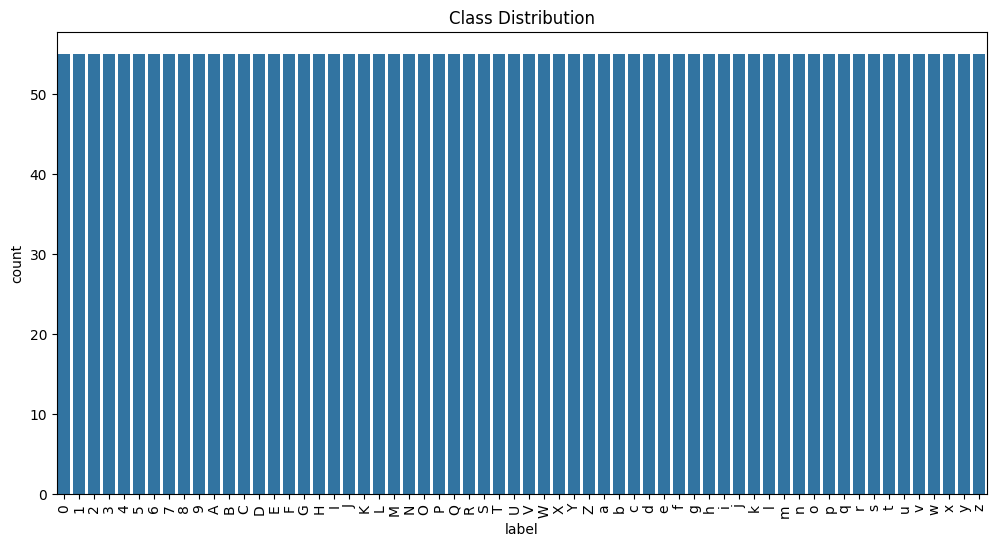
\includegraphics[width=469.5pt,height=257.8479pt]{latexImage_c67b9538e6e9b2c1250c3e8cd9729c53.png}}
\put(84,-651.3997){\fontsize{9.75}{1}\usefont{T1}{cmr}{m}{n}\selectfont\color{color_29791}Loading images...}
\put(84,-664.1498){\fontsize{9.75}{1}\usefont{T1}{cmr}{m}{n}\selectfont\color{color_29791}Training set: (2182, 1024), (2182,)}
\put(84,-676.8998){\fontsize{9.75}{1}\usefont{T1}{cmr}{m}{n}\selectfont\color{color_29791}Validation set: (546, 1024), (546,)}
\put(84,-689.6499){\fontsize{9.75}{1}\usefont{T1}{cmr}{m}{n}\selectfont\color{color_29791}Test set: (682, 1024), (682,)}
\end{picture}
\newpage
\begin{tikzpicture}[overlay]
\path(0pt,0pt);
\filldraw[color_283006][even odd rule]
(21pt, -746pt) -- (561pt, -746pt)
 -- (561pt, -746pt)
 -- (561pt, -26pt)
 -- (561pt, -26pt)
 -- (21pt, -26pt) -- cycle
;
\filldraw[color_273076][even odd rule]
(89.25pt, -731.072pt) -- (549.75pt, -731.072pt)
 -- (549.75pt, -731.072pt)
 -- (549.75pt, -110.0684pt)
 -- (549.75pt, -110.0684pt)
 -- (89.25pt, -110.0684pt) -- cycle
;
\filldraw[color_252223][nonzero rule]
(89.25pt, -731.072pt) -- (89.25pt, -110.0684pt)
 -- (89.25pt, -110.0684pt)
 -- (549.75pt, -110.0684pt)
 -- (549.75pt, -110.0684pt)
 -- (549.75pt, -731.072pt)
 -- (549.75pt, -731.072pt)
 -- (549pt, -731.072pt)
 -- (549pt, -731.072pt)
 -- (549pt, -110.8184pt)
 -- (549pt, -110.8184pt)
 -- (90pt, -110.8184pt)
 -- (90pt, -110.8184pt)
 -- (90pt, -731.072pt) -- cycle
;
\begin{scope}
\clip
(32.25pt, -731.072pt) -- (549.75pt, -731.072pt)
 -- (549.75pt, -731.072pt)
 -- (549.75pt, -110.0684pt)
 -- (549.75pt, -110.0684pt)
 -- (32.25pt, -110.0684pt) -- cycle
;
\begin{scope}
\clip
(90pt, -730.322pt) -- (549pt, -730.322pt)
 -- (549pt, -730.322pt)
 -- (549pt, -110.8184pt)
 -- (549pt, -110.8184pt)
 -- (90pt, -110.8184pt) -- cycle
;
\filldraw[color_273076][even odd rule]
(90pt, -730.322pt) -- (549pt, -730.322pt)
 -- (549pt, -730.322pt)
 -- (549pt, -110.8184pt)
 -- (549pt, -110.8184pt)
 -- (90pt, -110.8184pt) -- cycle
;
\end{scope}
\end{scope}
\begin{scope}
\clip
(32.25pt, -102.5684pt) -- (549.75pt, -102.5684pt)
 -- (549.75pt, -102.5684pt)
 -- (549.75pt, -37.25pt)
 -- (549.75pt, -37.25pt)
 -- (32.25pt, -37.25pt) -- cycle
;
\end{scope}
\end{tikzpicture}
\begin{picture}(-5,0)(2.5,0)
\put(93,-68.73761){\fontsize{21.7728}{1}\usefont{T1}{cmr}{m}{n}\selectfont\color{color_29791}**2. Perceptron Learning Algorithm}
\put(93,-90.51038){\fontsize{21.7728}{1}\usefont{T1}{cmr}{m}{n}\selectfont\color{color_29791}(PLA) Implementation and Results}
\put(93,-124.3188){\fontsize{9.75}{1}\usefont{T1}{cmr}{m}{n}\selectfont\color{color_95391}\# Perceptron Learning Algorithm (PLA) Implementation}
\put(93,-137.0689){\fontsize{9.75}{1}\usefont{T1}{cmr}{b}{n}\selectfont\color{color_33759}classPLA:}
\put(116.48,-149.819){\fontsize{9.75}{1}\usefont{T1}{cmr}{b}{n}\selectfont\color{color_33759}def\_\_init\_\_(self,input\_size,num\_classes,learning\_rate=0.01):}
\put(139.96,-162.569){\fontsize{9.75}{1}\usefont{T1}{cmr}{m}{n}\selectfont\color{color_62560}self.weights=np.zeros((num\_classes,input\_size))}
\put(139.96,-175.3191){\fontsize{9.75}{1}\usefont{T1}{cmr}{m}{n}\selectfont\color{color_62560}self.bias=np.zeros(num\_classes)}
\put(139.96,-188.0692){\fontsize{9.75}{1}\usefont{T1}{cmr}{m}{n}\selectfont\color{color_62560}self.learning\_rate=learning\_rate}
\put(139.96,-200.8193){\fontsize{9.75}{1}\usefont{T1}{cmr}{m}{n}\selectfont\color{color_62560}self.num\_classes=num\_classes}
\put(139.96,-213.5693){\fontsize{9.75}{1}\usefont{T1}{cmr}{m}{n}\selectfont\color{color_62560}self.train\_errors=[]\# To track training errors per epoch}
\put(116.48,-239.0695){\fontsize{9.75}{1}\usefont{T1}{cmr}{b}{n}\selectfont\color{color_33759}defstep\_activation(self,x):}
\put(139.96,-251.8196){\fontsize{9.75}{1}\usefont{T1}{cmr}{b}{n}\selectfont\color{color_33759}returnnp.where(x>=0,1,0)}
\put(116.48,-277.3197){\fontsize{9.75}{1}\usefont{T1}{cmr}{b}{n}\selectfont\color{color_33759}defpredict(self,x):}
\put(139.96,-290.0698){\fontsize{9.75}{1}\usefont{T1}{cmr}{m}{n}\selectfont\color{color_95391}\# One-vs-all approach for multiclass}
\put(139.96,-302.8199){\fontsize{9.75}{1}\usefont{T1}{cmr}{m}{n}\selectfont\color{color_62560}outputs=np.dot(self.weights,x)+self.bias}
\put(139.96,-315.5699){\fontsize{9.75}{1}\usefont{T1}{cmr}{b}{n}\selectfont\color{color_33759}returnnp.argmax(outputs)}
\put(116.48,-341.0701){\fontsize{9.75}{1}\usefont{T1}{cmr}{b}{n}\selectfont\color{color_33759}defpredict\_proba(self,x):}
\put(139.96,-353.8202){\fontsize{9.75}{1}\usefont{T1}{cmr}{m}{n}\selectfont\color{color_95391}\# For ROC curve, we need probability estimates}
\put(139.96,-366.5702){\fontsize{9.75}{1}\usefont{T1}{cmr}{m}{n}\selectfont\color{color_62560}outputs=np.dot(self.weights,x)+self.bias}
\put(139.96,-379.3203){\fontsize{9.75}{1}\usefont{T1}{cmr}{m}{n}\selectfont\color{color_95391}\# Simple softmax-like conversion (not exactly probabilities but works for ROC)}
\put(139.96,-392.0704){\fontsize{9.75}{1}\usefont{T1}{cmr}{m}{n}\selectfont\color{color_62560}exp\_outputs=np.exp(outputs-np.max(outputs))\# For numerical stability}
\put(139.96,-404.8205){\fontsize{9.75}{1}\usefont{T1}{cmr}{b}{n}\selectfont\color{color_33759}returnexp\_outputs/np.sum(exp\_outputs)}
\put(116.48,-430.3206){\fontsize{9.75}{1}\usefont{T1}{cmr}{b}{n}\selectfont\color{color_33759}deftrain(self,X,y,epochs=100):}
\put(139.96,-443.0707){\fontsize{9.75}{1}\usefont{T1}{cmr}{m}{n}\selectfont\color{color_62560}n\_samples=X.shape[0]}
\put(139.96,-468.5708){\fontsize{9.75}{1}\usefont{T1}{cmr}{b}{n}\selectfont\color{color_33759}forepochinrange(epochs):}
\put(163.4399,-481.3209){\fontsize{9.75}{1}\usefont{T1}{cmr}{m}{n}\selectfont\color{color_62560}errors=0}
\put(163.4399,-494.071){\fontsize{9.75}{1}\usefont{T1}{cmr}{b}{n}\selectfont\color{color_33759}foriinrange(n\_samples):}
\put(186.9199,-506.8211){\fontsize{9.75}{1}\usefont{T1}{cmr}{m}{n}\selectfont\color{color_62560}x\_i=X[i]}
\put(186.9199,-519.5711){\fontsize{9.75}{1}\usefont{T1}{cmr}{m}{n}\selectfont\color{color_62560}y\_true=y[i]}
\put(186.9199,-545.0713){\fontsize{9.75}{1}\usefont{T1}{cmr}{m}{n}\selectfont\color{color_95391}\# Prediction}
\put(186.9199,-557.8214){\fontsize{9.75}{1}\usefont{T1}{cmr}{m}{n}\selectfont\color{color_62560}y\_pred=self.predict(x\_i)}
\put(186.9199,-583.3215){\fontsize{9.75}{1}\usefont{T1}{cmr}{m}{n}\selectfont\color{color_95391}\# Update weights if prediction is wrong}
\put(186.9199,-596.0716){\fontsize{9.75}{1}\usefont{T1}{cmr}{b}{n}\selectfont\color{color_33759}ify\_pred!=y\_true:}
\put(210.3999,-608.8217){\fontsize{9.75}{1}\usefont{T1}{cmr}{m}{n}\selectfont\color{color_95391}\# Decrease score for wrong class}
\put(210.3999,-621.5717){\fontsize{9.75}{1}\usefont{T1}{cmr}{m}{n}\selectfont\color{color_62560}self.weights[y\_pred]-=self.learning\_rate*x\_i}
\put(210.3999,-634.3218){\fontsize{9.75}{1}\usefont{T1}{cmr}{m}{n}\selectfont\color{color_62560}self.bias[y\_pred]-=self.learning\_rate}
\put(210.3999,-659.822){\fontsize{9.75}{1}\usefont{T1}{cmr}{m}{n}\selectfont\color{color_95391}\# Increase score for correct class}
\put(210.3999,-672.572){\fontsize{9.75}{1}\usefont{T1}{cmr}{m}{n}\selectfont\color{color_62560}self.weights[y\_true]+=self.learning\_rate*x\_i}
\put(210.3999,-685.3221){\fontsize{9.75}{1}\usefont{T1}{cmr}{m}{n}\selectfont\color{color_62560}self.bias[y\_true]+=self.learning\_rate}
\put(210.3999,-710.8223){\fontsize{9.75}{1}\usefont{T1}{cmr}{m}{n}\selectfont\color{color_62560}errors+=1}
\put(43.66,-124.3188){\fontsize{9.75}{1}\usefont{T1}{cmr}{m}{n}\selectfont\color{color_126112}In[4]:}
\end{picture}
\newpage
\begin{tikzpicture}[overlay]
\path(0pt,0pt);
\filldraw[color_283006][even odd rule]
(21pt, -746pt) -- (561pt, -746pt)
 -- (561pt, -746pt)
 -- (561pt, -26pt)
 -- (561pt, -26pt)
 -- (21pt, -26pt) -- cycle
;
\filldraw[color_273076][even odd rule]
(89.25pt, -722.004pt) -- (549.75pt, -722.004pt)
 -- (549.75pt, -722.004pt)
 -- (549.75pt, -37.25pt)
 -- (549.75pt, -37.25pt)
 -- (89.25pt, -37.25pt) -- cycle
;
\filldraw[color_252223][nonzero rule]
(89.25pt, -722.004pt) -- (90pt, -722.004pt)
 -- (90pt, -722.004pt)
 -- (90pt, -37.25pt)
 -- (90pt, -37.25pt)
 -- (89.25pt, -37.25pt) -- cycle
;
\filldraw[color_252223][nonzero rule]
(549pt, -722.004pt) -- (549.75pt, -722.004pt)
 -- (549.75pt, -722.004pt)
 -- (549.75pt, -37.25pt)
 -- (549.75pt, -37.25pt)
 -- (549pt, -37.25pt) -- cycle
;
\begin{scope}
\clip
(32.25pt, -722.004pt) -- (549.75pt, -722.004pt)
 -- (549.75pt, -722.004pt)
 -- (549.75pt, -37.25pt)
 -- (549.75pt, -37.25pt)
 -- (32.25pt, -37.25pt) -- cycle
;
\begin{scope}
\clip
(90pt, -721.254pt) -- (549pt, -721.254pt)
 -- (549pt, -721.254pt)
 -- (549pt, -38pt)
 -- (549pt, -38pt)
 -- (90pt, -38pt) -- cycle
;
\filldraw[color_273076][even odd rule]
(90pt, -721.254pt) -- (549pt, -721.254pt)
 -- (549pt, -721.254pt)
 -- (549pt, -38pt)
 -- (549pt, -38pt)
 -- (90pt, -38pt) -- cycle
;
\end{scope}
\end{scope}
\begin{scope}
\clip
(32.25pt, -722.004pt) -- (549.75pt, -722.004pt)
 -- (549.75pt, -722.004pt)
 -- (549.75pt, -37.25pt)
 -- (549.75pt, -37.25pt)
 -- (32.25pt, -37.25pt) -- cycle
;
\begin{scope}
\clip
(90pt, -721.254pt) -- (549pt, -721.254pt)
 -- (549pt, -721.254pt)
 -- (549pt, -38pt)
 -- (549pt, -38pt)
 -- (90pt, -38pt) -- cycle
;
\end{scope}
\end{scope}
\end{tikzpicture}
\begin{picture}(-5,0)(2.5,0)
\put(163.4399,-51.50043){\fontsize{9.75}{1}\usefont{T1}{cmr}{m}{n}\selectfont\color{color_95391}\# Record error rate for this epoch}
\put(163.4399,-64.25049){\fontsize{9.75}{1}\usefont{T1}{cmr}{m}{n}\selectfont\color{color_62560}error\_rate=errors/n\_samples}
\put(163.4399,-77.00061){\fontsize{9.75}{1}\usefont{T1}{cmr}{m}{n}\selectfont\color{color_62560}self.train\_errors.append(error\_rate)}
\put(163.4399,-102.5007){\fontsize{9.75}{1}\usefont{T1}{cmr}{m}{n}\selectfont\color{color_95391}\# Print progress}
\put(163.4399,-115.2508){\fontsize{9.75}{1}\usefont{T1}{cmr}{b}{n}\selectfont\color{color_33759}if(epoch+1)\%10==0:}
\put(186.9199,-128.0009){\fontsize{9.75}{1}\usefont{T1}{cmr}{m}{n}\selectfont\color{color_62560}print(f"Epoch\{epoch+1\}/\{epochs\}, Error Rate:\{error\_rate:.4f\}"}
\put(163.4399,-153.501){\fontsize{9.75}{1}\usefont{T1}{cmr}{m}{n}\selectfont\color{color_95391}\# Early stopping if no errors}
\put(163.4399,-166.2511){\fontsize{9.75}{1}\usefont{T1}{cmr}{b}{n}\selectfont\color{color_33759}iferrors==0:}
\put(186.9199,-179.0012){\fontsize{9.75}{1}\usefont{T1}{cmr}{m}{n}\selectfont\color{color_62560}print(f"Converged at epoch\{epoch+1\}")}
\put(186.9199,-191.7512){\fontsize{9.75}{1}\usefont{T1}{cmr}{b}{n}\selectfont\color{color_33759}break}
\put(116.48,-217.2514){\fontsize{9.75}{1}\usefont{T1}{cmr}{b}{n}\selectfont\color{color_33759}defevaluate(self,X,y):}
\put(139.96,-230.0015){\fontsize{9.75}{1}\usefont{T1}{cmr}{m}{n}\selectfont\color{color_62560}n\_samples=X.shape[0]}
\put(139.96,-242.7515){\fontsize{9.75}{1}\usefont{T1}{cmr}{m}{n}\selectfont\color{color_62560}y\_pred=[]}
\put(139.96,-255.5016){\fontsize{9.75}{1}\usefont{T1}{cmr}{m}{n}\selectfont\color{color_62560}y\_proba=[]}
\put(139.96,-281.0018){\fontsize{9.75}{1}\usefont{T1}{cmr}{b}{n}\selectfont\color{color_33759}foriinrange(n\_samples):}
\put(163.4399,-293.7518){\fontsize{9.75}{1}\usefont{T1}{cmr}{m}{n}\selectfont\color{color_62560}pred=self.predict(X[i])}
\put(163.4399,-306.5019){\fontsize{9.75}{1}\usefont{T1}{cmr}{m}{n}\selectfont\color{color_62560}y\_pred.append(pred)}
\put(163.4399,-319.252){\fontsize{9.75}{1}\usefont{T1}{cmr}{m}{n}\selectfont\color{color_62560}y\_proba.append(self.predict\_proba(X[i]))}
\put(139.96,-344.7521){\fontsize{9.75}{1}\usefont{T1}{cmr}{b}{n}\selectfont\color{color_33759}returnnp.array(y\_pred),np.array(y\_proba)}
\put(93,-370.2523){\fontsize{9.75}{1}\usefont{T1}{cmr}{m}{n}\selectfont\color{color_95391}\# Initialize and train PLA}
\put(93,-383.0024){\fontsize{9.75}{1}\usefont{T1}{cmr}{m}{n}\selectfont\color{color_62560}print("Training PLA...")}
\put(93,-395.7524){\fontsize{9.75}{1}\usefont{T1}{cmr}{m}{n}\selectfont\color{color_62560}input\_size=X\_train.shape[1]}
\put(93,-408.5025){\fontsize{9.75}{1}\usefont{T1}{cmr}{m}{n}\selectfont\color{color_62560}num\_classes=len(np.unique(y\_train))}
\put(93,-434.0027){\fontsize{9.75}{1}\usefont{T1}{cmr}{m}{n}\selectfont\color{color_62560}pla=PLA(input\_size,num\_classes,learning\_rate=0.01)}
\put(93,-446.7527){\fontsize{9.75}{1}\usefont{T1}{cmr}{m}{n}\selectfont\color{color_62560}pla.train(X\_train,y\_train,epochs=100)}
\put(93,-472.2529){\fontsize{9.75}{1}\usefont{T1}{cmr}{m}{n}\selectfont\color{color_95391}\# Plot PLA training convergence}
\put(93,-485.003){\fontsize{9.75}{1}\usefont{T1}{cmr}{m}{n}\selectfont\color{color_62560}plt.figure(figsize=(10,6))}
\put(93,-497.753){\fontsize{9.75}{1}\usefont{T1}{cmr}{m}{n}\selectfont\color{color_62560}plt.plot(pla.train\_errors)}
\put(93,-510.5031){\fontsize{9.75}{1}\usefont{T1}{cmr}{m}{n}\selectfont\color{color_62560}plt.title('PLA Training Error Convergence')}
\put(93,-523.2532){\fontsize{9.75}{1}\usefont{T1}{cmr}{m}{n}\selectfont\color{color_62560}plt.xlabel('Epoch')}
\put(93,-536.0033){\fontsize{9.75}{1}\usefont{T1}{cmr}{m}{n}\selectfont\color{color_62560}plt.ylabel('Error Rate')}
\put(93,-548.7533){\fontsize{9.75}{1}\usefont{T1}{cmr}{m}{n}\selectfont\color{color_62560}plt.grid(True)}
\put(93,-561.5034){\fontsize{9.75}{1}\usefont{T1}{cmr}{m}{n}\selectfont\color{color_62560}plt.show()}
\put(93,-587.0036){\fontsize{9.75}{1}\usefont{T1}{cmr}{m}{n}\selectfont\color{color_95391}\# Evaluate PLA}
\put(93,-599.7536){\fontsize{9.75}{1}\usefont{T1}{cmr}{m}{n}\selectfont\color{color_62560}y\_pred\_pla,y\_proba\_pla=pla.evaluate(X\_test,y\_test)}
\put(93,-612.5037){\fontsize{9.75}{1}\usefont{T1}{cmr}{m}{n}\selectfont\color{color_62560}pla\_accuracy=accuracy\_score(y\_test,y\_pred\_pla)}
\put(93,-625.2538){\fontsize{9.75}{1}\usefont{T1}{cmr}{m}{n}\selectfont\color{color_62560}pla\_precision=precision\_score(y\_test,y\_pred\_pla,average='weighted',zero\_division}
\put(93,-638.0039){\fontsize{9.75}{1}\usefont{T1}{cmr}{m}{n}\selectfont\color{color_62560}pla\_recall=recall\_score(y\_test,y\_pred\_pla,average='weighted',zero\_division}
\put(93,-650.7539){\fontsize{9.75}{1}\usefont{T1}{cmr}{m}{n}\selectfont\color{color_62560}pla\_f1=f1\_score(y\_test,y\_pred\_pla,average='weighted',zero\_division=0)}
\put(93,-676.2541){\fontsize{9.75}{1}\usefont{T1}{cmr}{m}{n}\selectfont\color{color_62560}print(f"PLA Test Accuracy:\{pla\_accuracy:.4f\}")}
\put(93,-689.0042){\fontsize{9.75}{1}\usefont{T1}{cmr}{m}{n}\selectfont\color{color_62560}print(f"PLA Test Precision:\{pla\_precision:.4f\}")}
\put(93,-701.7542){\fontsize{9.75}{1}\usefont{T1}{cmr}{m}{n}\selectfont\color{color_62560}print(f"PLA Test Recall:\{pla\_recall:.4f\}")}
\put(93,-714.5043){\fontsize{9.75}{1}\usefont{T1}{cmr}{m}{n}\selectfont\color{color_62560}print(f"PLA Test F1-Score:\{pla\_f1:.4f\}")}
\end{picture}
\newpage
\begin{tikzpicture}[overlay]
\path(0pt,0pt);
\filldraw[color_283006][even odd rule]
(21pt, -746pt) -- (561pt, -746pt)
 -- (561pt, -746pt)
 -- (561pt, -26pt)
 -- (561pt, -26pt)
 -- (21pt, -26pt) -- cycle
;
\filldraw[color_273076][even odd rule]
(89.25pt, -518.0028pt) -- (549.75pt, -518.0028pt)
 -- (549.75pt, -518.0028pt)
 -- (549.75pt, -37.25pt)
 -- (549.75pt, -37.25pt)
 -- (89.25pt, -37.25pt) -- cycle
;
\filldraw[color_252223][nonzero rule]
(549.75pt, -37.25pt) -- (549.75pt, -518.0028pt)
 -- (549.75pt, -518.0028pt)
 -- (89.25pt, -518.0028pt)
 -- (89.25pt, -518.0028pt)
 -- (89.25pt, -37.25pt)
 -- (89.25pt, -37.25pt)
 -- (90pt, -37.25pt)
 -- (90pt, -37.25pt)
 -- (90pt, -517.2528pt)
 -- (90pt, -517.2528pt)
 -- (549pt, -517.2528pt)
 -- (549pt, -517.2528pt)
 -- (549pt, -37.25pt) -- cycle
;
\begin{scope}
\clip
(32.25pt, -518.0028pt) -- (549.75pt, -518.0028pt)
 -- (549.75pt, -518.0028pt)
 -- (549.75pt, -37.25pt)
 -- (549.75pt, -37.25pt)
 -- (32.25pt, -37.25pt) -- cycle
;
\begin{scope}
\clip
(90pt, -517.2528pt) -- (549pt, -517.2528pt)
 -- (549pt, -517.2528pt)
 -- (549pt, -38pt)
 -- (549pt, -38pt)
 -- (90pt, -38pt) -- cycle
;
\filldraw[color_273076][even odd rule]
(90pt, -517.2528pt) -- (549pt, -517.2528pt)
 -- (549pt, -517.2528pt)
 -- (549pt, -38pt)
 -- (549pt, -38pt)
 -- (90pt, -38pt) -- cycle
;
\end{scope}
\end{scope}
\begin{scope}
\clip
(32.25pt, -518.0028pt) -- (549.75pt, -518.0028pt)
 -- (549.75pt, -518.0028pt)
 -- (549.75pt, -37.25pt)
 -- (549.75pt, -37.25pt)
 -- (32.25pt, -37.25pt) -- cycle
;
\begin{scope}
\clip
(90pt, -517.2528pt) -- (549pt, -517.2528pt)
 -- (549pt, -517.2528pt)
 -- (549pt, -38pt)
 -- (549pt, -38pt)
 -- (90pt, -38pt) -- cycle
;
\end{scope}
\end{scope}
\end{tikzpicture}
\begin{picture}(-5,0)(2.5,0)
\put(93,-64.25049){\fontsize{9.75}{1}\usefont{T1}{cmr}{m}{n}\selectfont\color{color_95391}\# Confusion matrix for PLA}
\put(93,-77.00061){\fontsize{9.75}{1}\usefont{T1}{cmr}{m}{n}\selectfont\color{color_62560}plt.figure(figsize=(10,8))}
\put(93,-89.75061){\fontsize{9.75}{1}\usefont{T1}{cmr}{m}{n}\selectfont\color{color_62560}cm\_pla=confusion\_matrix(y\_test,y\_pred\_pla)}
\put(93,-102.5007){\fontsize{9.75}{1}\usefont{T1}{cmr}{m}{n}\selectfont\color{color_62560}sns.heatmap(cm\_pla,annot=False,fmt='d',cmap='Blues')}
\put(93,-115.2508){\fontsize{9.75}{1}\usefont{T1}{cmr}{m}{n}\selectfont\color{color_62560}plt.title('PLA Confusion Matrix')}
\put(93,-128.0009){\fontsize{9.75}{1}\usefont{T1}{cmr}{m}{n}\selectfont\color{color_62560}plt.ylabel('True Label')}
\put(93,-140.7509){\fontsize{9.75}{1}\usefont{T1}{cmr}{m}{n}\selectfont\color{color_62560}plt.xlabel('Predicted Label')}
\put(93,-153.501){\fontsize{9.75}{1}\usefont{T1}{cmr}{m}{n}\selectfont\color{color_62560}plt.show()}
\put(93,-179.0012){\fontsize{9.75}{1}\usefont{T1}{cmr}{m}{n}\selectfont\color{color_95391}\# Classification report for PLA}
\put(93,-191.7512){\fontsize{9.75}{1}\usefont{T1}{cmr}{m}{n}\selectfont\color{color_62560}class\_names=label\_encoder.classes\_}
\put(93,-204.5013){\fontsize{9.75}{1}\usefont{T1}{cmr}{m}{n}\selectfont\color{color_62560}print("\nClassification Report for PLA:")}
\put(93,-217.2514){\fontsize{9.75}{1}\usefont{T1}{cmr}{m}{n}\selectfont\color{color_62560}print(classification\_report(y\_test,y\_pred\_pla,target\_names=class\_names,zero\_division}
\put(93,-242.7515){\fontsize{9.75}{1}\usefont{T1}{cmr}{m}{n}\selectfont\color{color_95391}\# Visualize some PLA predictions}
\put(93,-255.5016){\fontsize{9.75}{1}\usefont{T1}{cmr}{b}{n}\selectfont\color{color_33759}defvisualize\_pla\_predictions(pla\_model,X,y,label\_encoder,num\_samples=10):}
\put(116.48,-268.2517){\fontsize{9.75}{1}\usefont{T1}{cmr}{m}{n}\selectfont\color{color_62560}plt.figure(figsize=(15,6))}
\put(116.48,-281.0018){\fontsize{9.75}{1}\usefont{T1}{cmr}{m}{n}\selectfont\color{color_62560}indices=np.random.choice(len(X),num\_samples,replace=False)}
\put(116.48,-306.5019){\fontsize{9.75}{1}\usefont{T1}{cmr}{b}{n}\selectfont\color{color_33759}fori,idxinenumerate(indices):}
\put(139.96,-319.252){\fontsize{9.75}{1}\usefont{T1}{cmr}{m}{n}\selectfont\color{color_62560}plt.subplot(2,5,i+1)}
\put(139.96,-332.0021){\fontsize{9.75}{1}\usefont{T1}{cmr}{m}{n}\selectfont\color{color_95391}\# Reshape flattened image to 2D (assuming original was 32x32)}
\put(139.96,-344.7521){\fontsize{9.75}{1}\usefont{T1}{cmr}{m}{n}\selectfont\color{color_62560}img=X[idx].reshape(32,32)}
\put(139.96,-357.5022){\fontsize{9.75}{1}\usefont{T1}{cmr}{m}{n}\selectfont\color{color_62560}plt.imshow(img,cmap='gray')}
\put(139.96,-383.0024){\fontsize{9.75}{1}\usefont{T1}{cmr}{m}{n}\selectfont\color{color_62560}true\_label=label\_encoder.inverse\_transform([y[idx]])[0]}
\put(139.96,-395.7524){\fontsize{9.75}{1}\usefont{T1}{cmr}{m}{n}\selectfont\color{color_62560}pred\_label=label\_encoder.inverse\_transform([pla\_model.predict(X[idx])])[}
\put(139.96,-421.2526){\fontsize{9.75}{1}\usefont{T1}{cmr}{m}{n}\selectfont\color{color_62560}title\_color='green'iftrue\_label==pred\_labelelse'red'}
\put(139.96,-434.0027){\fontsize{9.75}{1}\usefont{T1}{cmr}{m}{n}\selectfont\color{color_62560}plt.title(f"True:\{true\_label\}\nPred:\{pred\_label\}",color=title\_color)}
\put(139.96,-446.7527){\fontsize{9.75}{1}\usefont{T1}{cmr}{m}{n}\selectfont\color{color_62560}plt.axis('off')}
\put(116.48,-472.2529){\fontsize{9.75}{1}\usefont{T1}{cmr}{m}{n}\selectfont\color{color_62560}plt.tight\_layout()}
\put(116.48,-485.003){\fontsize{9.75}{1}\usefont{T1}{cmr}{m}{n}\selectfont\color{color_62560}plt.show()}
\put(93,-510.5031){\fontsize{9.75}{1}\usefont{T1}{cmr}{m}{n}\selectfont\color{color_62560}visualize\_pla\_predictions(pla,X\_test,y\_test,label\_encoder)}
\put(84,-531.5032){\fontsize{9.75}{1}\usefont{T1}{cmr}{m}{n}\selectfont\color{color_29791}Training PLA...}
\put(84,-544.2533){\fontsize{9.75}{1}\usefont{T1}{cmr}{m}{n}\selectfont\color{color_29791}Epoch 10/100, Error Rate: 0.3639}
\put(84,-557.0033){\fontsize{9.75}{1}\usefont{T1}{cmr}{m}{n}\selectfont\color{color_29791}Epoch 20/100, Error Rate: 0.2273}
\put(84,-569.7534){\fontsize{9.75}{1}\usefont{T1}{cmr}{m}{n}\selectfont\color{color_29791}Epoch 30/100, Error Rate: 0.1320}
\put(84,-582.5035){\fontsize{9.75}{1}\usefont{T1}{cmr}{m}{n}\selectfont\color{color_29791}Epoch 40/100, Error Rate: 0.0930}
\put(84,-595.2536){\fontsize{9.75}{1}\usefont{T1}{cmr}{m}{n}\selectfont\color{color_29791}Epoch 50/100, Error Rate: 0.0687}
\put(84,-608.0036){\fontsize{9.75}{1}\usefont{T1}{cmr}{m}{n}\selectfont\color{color_29791}Epoch 60/100, Error Rate: 0.0733}
\put(84,-620.7537){\fontsize{9.75}{1}\usefont{T1}{cmr}{m}{n}\selectfont\color{color_29791}Epoch 70/100, Error Rate: 0.0371}
\put(84,-633.5038){\fontsize{9.75}{1}\usefont{T1}{cmr}{m}{n}\selectfont\color{color_29791}Epoch 80/100, Error Rate: 0.0367}
\put(84,-646.2539){\fontsize{9.75}{1}\usefont{T1}{cmr}{m}{n}\selectfont\color{color_29791}Epoch 90/100, Error Rate: 0.0316}
\put(84,-659.0039){\fontsize{9.75}{1}\usefont{T1}{cmr}{m}{n}\selectfont\color{color_29791}Epoch 100/100, Error Rate: 0.0234}
\end{picture}
\newpage
\begin{tikzpicture}[overlay]
\path(0pt,0pt);
\filldraw[color_283006][even odd rule]
(21pt, -746pt) -- (561pt, -746pt)
 -- (561pt, -746pt)
 -- (561pt, -26pt)
 -- (561pt, -26pt)
 -- (21pt, -26pt) -- cycle
;
\begin{scope}
\clip
(32.25pt, -346.865pt) -- (549.75pt, -346.865pt)
 -- (549.75pt, -346.865pt)
 -- (549.75pt, -41pt)
 -- (549.75pt, -41pt)
 -- (32.25pt, -41pt) -- cycle
;
\end{scope}
\end{tikzpicture}
\begin{picture}(-5,0)(2.5,0)
\put(80.25,-344.5656){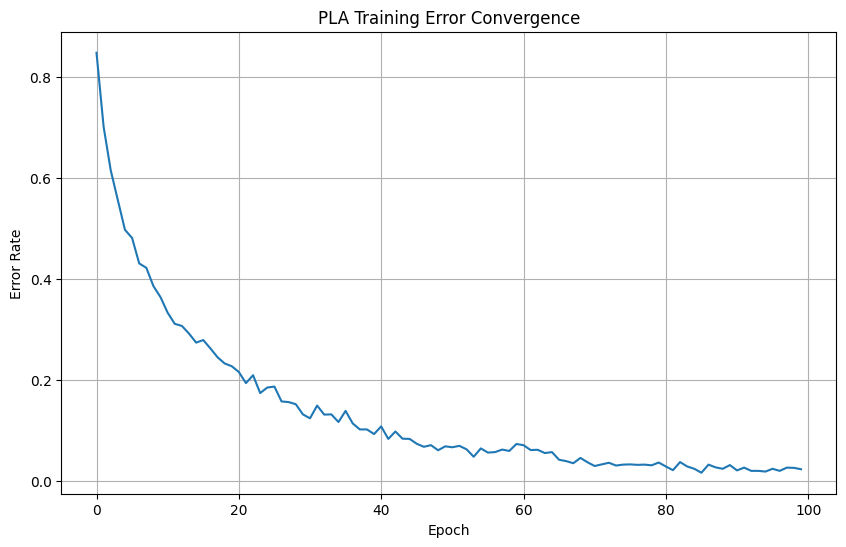
\includegraphics[width=469.5pt,height=303.5656pt]{latexImage_933bc55039682f3e695fcad13dc8598c.png}}
\put(84,-356.6154){\fontsize{9.75}{1}\usefont{T1}{cmr}{m}{n}\selectfont\color{color_29791}PLA Test Accuracy: 0.2419}
\put(84,-369.3655){\fontsize{9.75}{1}\usefont{T1}{cmr}{m}{n}\selectfont\color{color_29791}PLA Test Precision: 0.2491}
\put(84,-382.1156){\fontsize{9.75}{1}\usefont{T1}{cmr}{m}{n}\selectfont\color{color_29791}PLA Test Recall: 0.2419}
\put(84,-394.8657){\fontsize{9.75}{1}\usefont{T1}{cmr}{m}{n}\selectfont\color{color_29791}PLA Test F1-Score: 0.2410}
\end{picture}
\newpage
\begin{tikzpicture}[overlay]
\path(0pt,0pt);
\filldraw[color_283006][even odd rule]
(21pt, -746pt) -- (561pt, -746pt)
 -- (561pt, -746pt)
 -- (561pt, -26pt)
 -- (561pt, -26pt)
 -- (21pt, -26pt) -- cycle
;
\begin{scope}
\clip
(32.25pt, -470.173pt) -- (549.75pt, -470.173pt)
 -- (549.75pt, -470.173pt)
 -- (549.75pt, -41pt)
 -- (549.75pt, -41pt)
 -- (32.25pt, -41pt) -- cycle
;
\end{scope}
\end{tikzpicture}
\begin{picture}(-5,0)(2.5,0)
\put(80.25,-467.8735){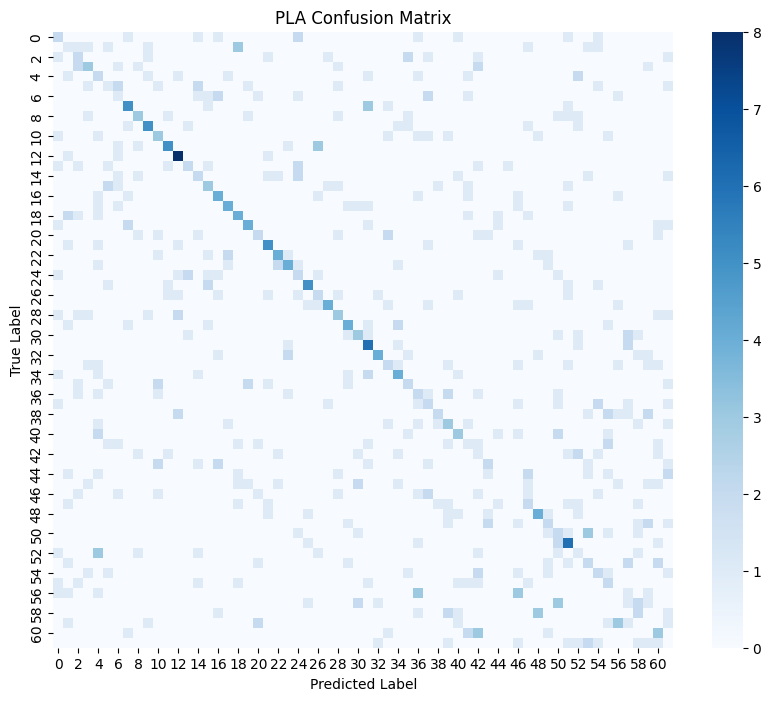
\includegraphics[width=469.5pt,height=426.8735pt]{latexImage_b42771bb193e8c4e53b22bb794cdfeba.png}}
\end{picture}
\newpage
\begin{tikzpicture}[overlay]
\path(0pt,0pt);
\filldraw[color_283006][even odd rule]
(21pt, -746pt) -- (561pt, -746pt)
 -- (561pt, -746pt)
 -- (561pt, -26pt)
 -- (561pt, -26pt)
 -- (21pt, -26pt) -- cycle
;
\begin{scope}
\clip
(32.25pt, -729.5041pt) -- (549.75pt, -729.5041pt)
 -- (549.75pt, -729.5041pt)
 -- (549.75pt, -41pt)
 -- (549.75pt, -41pt)
 -- (32.25pt, -41pt) -- cycle
;
\end{scope}
\end{tikzpicture}
\begin{picture}(-5,0)(2.5,0)
\put(84,-50.75043){\fontsize{9.75}{1}\usefont{T1}{cmr}{m}{n}\selectfont\color{color_29791}Classification Report for PLA:}
\put(166.1799,-63.50049){\fontsize{9.75}{1}\usefont{T1}{cmr}{m}{n}\selectfont\color{color_29791}precision    recall  f1-score   support}
\put(148.5699,-89.00061){\fontsize{9.75}{1}\usefont{T1}{cmr}{m}{n}\selectfont\color{color_29791}0       0.15      0.18      0.17        11}
\put(148.5699,-101.7507){\fontsize{9.75}{1}\usefont{T1}{cmr}{m}{n}\selectfont\color{color_29791}1       0.08      0.09      0.09        11}
\put(148.5699,-114.5008){\fontsize{9.75}{1}\usefont{T1}{cmr}{m}{n}\selectfont\color{color_29791}2       0.17      0.18      0.17        11}
\put(148.5699,-127.2509){\fontsize{9.75}{1}\usefont{T1}{cmr}{m}{n}\selectfont\color{color_29791}3       0.30      0.27      0.29        11}
\put(148.5699,-140.0009){\fontsize{9.75}{1}\usefont{T1}{cmr}{m}{n}\selectfont\color{color_29791}4       0.11      0.18      0.13        11}
\put(148.5699,-152.751){\fontsize{9.75}{1}\usefont{T1}{cmr}{m}{n}\selectfont\color{color_29791}5       0.11      0.09      0.10        11}
\put(148.5699,-165.5011){\fontsize{9.75}{1}\usefont{T1}{cmr}{m}{n}\selectfont\color{color_29791}6       0.09      0.09      0.09        11}
\put(148.5699,-178.2512){\fontsize{9.75}{1}\usefont{T1}{cmr}{m}{n}\selectfont\color{color_29791}7       0.42      0.45      0.43        11}
\put(148.5699,-191.0012){\fontsize{9.75}{1}\usefont{T1}{cmr}{m}{n}\selectfont\color{color_29791}8       0.33      0.27      0.30        11}
\put(148.5699,-203.7513){\fontsize{9.75}{1}\usefont{T1}{cmr}{m}{n}\selectfont\color{color_29791}9       0.50      0.45      0.48        11}
\put(148.5699,-216.5014){\fontsize{9.75}{1}\usefont{T1}{cmr}{m}{n}\selectfont\color{color_29791}A       0.25      0.27      0.26        11}
\put(148.5699,-229.2515){\fontsize{9.75}{1}\usefont{T1}{cmr}{m}{n}\selectfont\color{color_29791}B       0.50      0.45      0.48        11}
\put(148.5699,-242.0015){\fontsize{9.75}{1}\usefont{T1}{cmr}{m}{n}\selectfont\color{color_29791}C       0.50      0.73      0.59        11}
\put(148.5699,-254.7516){\fontsize{9.75}{1}\usefont{T1}{cmr}{m}{n}\selectfont\color{color_29791}D       0.33      0.18      0.24        11}
\put(148.5699,-267.5017){\fontsize{9.75}{1}\usefont{T1}{cmr}{m}{n}\selectfont\color{color_29791}E       0.18      0.18      0.18        11}
\put(148.5699,-280.2518){\fontsize{9.75}{1}\usefont{T1}{cmr}{m}{n}\selectfont\color{color_29791}F       0.27      0.27      0.27        11}
\put(148.5699,-293.0018){\fontsize{9.75}{1}\usefont{T1}{cmr}{m}{n}\selectfont\color{color_29791}G       0.31      0.36      0.33        11}
\put(148.5699,-305.7519){\fontsize{9.75}{1}\usefont{T1}{cmr}{m}{n}\selectfont\color{color_29791}H       0.44      0.36      0.40        11}
\put(148.5699,-318.502){\fontsize{9.75}{1}\usefont{T1}{cmr}{m}{n}\selectfont\color{color_29791}I       0.33      0.36      0.35        11}
\put(148.5699,-331.2521){\fontsize{9.75}{1}\usefont{T1}{cmr}{m}{n}\selectfont\color{color_29791}J       0.44      0.36      0.40        11}
\put(148.5699,-344.0021){\fontsize{9.75}{1}\usefont{T1}{cmr}{m}{n}\selectfont\color{color_29791}K       0.25      0.18      0.21        11}
\put(148.5699,-356.7522){\fontsize{9.75}{1}\usefont{T1}{cmr}{m}{n}\selectfont\color{color_29791}L       0.42      0.45      0.43        11}
\put(148.5699,-369.5023){\fontsize{9.75}{1}\usefont{T1}{cmr}{m}{n}\selectfont\color{color_29791}M       0.44      0.36      0.40        11}
\put(148.5699,-382.2524){\fontsize{9.75}{1}\usefont{T1}{cmr}{m}{n}\selectfont\color{color_29791}N       0.40      0.36      0.38        11}
\put(148.5699,-395.0024){\fontsize{9.75}{1}\usefont{T1}{cmr}{m}{n}\selectfont\color{color_29791}O       0.17      0.18      0.17        11}
\put(148.5699,-407.7525){\fontsize{9.75}{1}\usefont{T1}{cmr}{m}{n}\selectfont\color{color_29791}P       0.56      0.45      0.50        11}
\put(148.5699,-420.5026){\fontsize{9.75}{1}\usefont{T1}{cmr}{m}{n}\selectfont\color{color_29791}Q       0.22      0.18      0.20        11}
\put(148.5699,-433.2527){\fontsize{9.75}{1}\usefont{T1}{cmr}{m}{n}\selectfont\color{color_29791}R       0.57      0.36      0.44        11}
\put(148.5699,-446.0027){\fontsize{9.75}{1}\usefont{T1}{cmr}{m}{n}\selectfont\color{color_29791}S       0.27      0.27      0.27        11}
\put(148.5699,-458.7528){\fontsize{9.75}{1}\usefont{T1}{cmr}{m}{n}\selectfont\color{color_29791}T       0.40      0.36      0.38        11}
\put(148.5699,-471.5029){\fontsize{9.75}{1}\usefont{T1}{cmr}{m}{n}\selectfont\color{color_29791}U       0.30      0.27      0.29        11}
\put(148.5699,-484.253){\fontsize{9.75}{1}\usefont{T1}{cmr}{m}{n}\selectfont\color{color_29791}V       0.32      0.55      0.40        11}
\put(148.5699,-497.003){\fontsize{9.75}{1}\usefont{T1}{cmr}{m}{n}\selectfont\color{color_29791}W       0.57      0.36      0.44        11}
\put(148.5699,-509.7531){\fontsize{9.75}{1}\usefont{T1}{cmr}{m}{n}\selectfont\color{color_29791}X       0.22      0.18      0.20        11}
\put(148.5699,-522.5032){\fontsize{9.75}{1}\usefont{T1}{cmr}{m}{n}\selectfont\color{color_29791}Y       0.33      0.36      0.35        11}
\put(148.5699,-535.2533){\fontsize{9.75}{1}\usefont{T1}{cmr}{m}{n}\selectfont\color{color_29791}Z       0.22      0.18      0.20        11}
\put(148.5699,-548.0033){\fontsize{9.75}{1}\usefont{T1}{cmr}{m}{n}\selectfont\color{color_29791}a       0.14      0.18      0.16        11}
\put(148.5699,-560.7534){\fontsize{9.75}{1}\usefont{T1}{cmr}{m}{n}\selectfont\color{color_29791}b       0.17      0.18      0.17        11}
\put(148.5699,-573.5035){\fontsize{9.75}{1}\usefont{T1}{cmr}{m}{n}\selectfont\color{color_29791}c       0.40      0.18      0.25        11}
\put(148.5699,-586.2536){\fontsize{9.75}{1}\usefont{T1}{cmr}{m}{n}\selectfont\color{color_29791}d       0.21      0.27      0.24        11}
\put(148.5699,-599.0036){\fontsize{9.75}{1}\usefont{T1}{cmr}{m}{n}\selectfont\color{color_29791}e       0.27      0.27      0.27        11}
\put(148.5699,-611.7537){\fontsize{9.75}{1}\usefont{T1}{cmr}{m}{n}\selectfont\color{color_29791}f       0.10      0.09      0.10        11}
\put(148.5699,-624.5038){\fontsize{9.75}{1}\usefont{T1}{cmr}{m}{n}\selectfont\color{color_29791}g       0.06      0.09      0.07        11}
\put(148.5699,-637.2539){\fontsize{9.75}{1}\usefont{T1}{cmr}{m}{n}\selectfont\color{color_29791}h       0.29      0.18      0.22        11}
\put(148.5699,-650.0039){\fontsize{9.75}{1}\usefont{T1}{cmr}{m}{n}\selectfont\color{color_29791}i       0.00      0.00      0.00        11}
\put(148.5699,-662.754){\fontsize{9.75}{1}\usefont{T1}{cmr}{m}{n}\selectfont\color{color_29791}j       0.00      0.00      0.00        11}
\put(148.5699,-675.5041){\fontsize{9.75}{1}\usefont{T1}{cmr}{m}{n}\selectfont\color{color_29791}k       0.00      0.00      0.00        11}
\put(148.5699,-688.2542){\fontsize{9.75}{1}\usefont{T1}{cmr}{m}{n}\selectfont\color{color_29791}l       0.18      0.18      0.18        11}
\put(148.5699,-701.0042){\fontsize{9.75}{1}\usefont{T1}{cmr}{m}{n}\selectfont\color{color_29791}m       0.40      0.36      0.38        11}
\put(148.5699,-713.7543){\fontsize{9.75}{1}\usefont{T1}{cmr}{m}{n}\selectfont\color{color_29791}n       0.22      0.18      0.20        11}
\put(148.5699,-726.5044){\fontsize{9.75}{1}\usefont{T1}{cmr}{m}{n}\selectfont\color{color_29791}o       0.13      0.18      0.15        11}
\end{picture}
\newpage
\begin{tikzpicture}[overlay]
\path(0pt,0pt);
\filldraw[color_283006][even odd rule]
(21pt, -746pt) -- (561pt, -746pt)
 -- (561pt, -746pt)
 -- (561pt, -26pt)
 -- (561pt, -26pt)
 -- (21pt, -26pt) -- cycle
;
\filldraw[color_273076][even odd rule]
(89.25pt, -724.0634pt) -- (549.75pt, -724.0634pt)
 -- (549.75pt, -724.0634pt)
 -- (549.75pt, -498.3121pt)
 -- (549.75pt, -498.3121pt)
 -- (89.25pt, -498.3121pt) -- cycle
;
\filldraw[color_252223][nonzero rule]
(89.25pt, -724.0634pt) -- (89.25pt, -498.3121pt)
 -- (89.25pt, -498.3121pt)
 -- (549.75pt, -498.3121pt)
 -- (549.75pt, -498.3121pt)
 -- (549.75pt, -724.0634pt)
 -- (549.75pt, -724.0634pt)
 -- (549pt, -724.0634pt)
 -- (549pt, -724.0634pt)
 -- (549pt, -499.0621pt)
 -- (549pt, -499.0621pt)
 -- (90pt, -499.0621pt)
 -- (90pt, -499.0621pt)
 -- (90pt, -724.0634pt) -- cycle
;
\begin{scope}
\clip
(32.25pt, -724.0634pt) -- (549.75pt, -724.0634pt)
 -- (549.75pt, -724.0634pt)
 -- (549.75pt, -498.3121pt)
 -- (549.75pt, -498.3121pt)
 -- (32.25pt, -498.3121pt) -- cycle
;
\begin{scope}
\clip
(90pt, -723.3134pt) -- (549pt, -723.3134pt)
 -- (549pt, -723.3134pt)
 -- (549pt, -499.0621pt)
 -- (549pt, -499.0621pt)
 -- (90pt, -499.0621pt) -- cycle
;
\filldraw[color_273076][even odd rule]
(90pt, -723.3134pt) -- (549pt, -723.3134pt)
 -- (549pt, -723.3134pt)
 -- (549pt, -499.0621pt)
 -- (549pt, -499.0621pt)
 -- (90pt, -499.0621pt) -- cycle
;
\end{scope}
\end{scope}
\begin{scope}
\clip
(32.25pt, -245.0012pt) -- (549.75pt, -245.0012pt)
 -- (549.75pt, -245.0012pt)
 -- (549.75pt, -41pt)
 -- (549.75pt, -41pt)
 -- (32.25pt, -41pt) -- cycle
;
\end{scope}
\end{tikzpicture}
\begin{picture}(-5,0)(2.5,0)
\put(148.5699,-50.75043){\fontsize{9.75}{1}\usefont{T1}{cmr}{m}{n}\selectfont\color{color_29791}p       0.32      0.55      0.40        11}
\put(148.5699,-63.50049){\fontsize{9.75}{1}\usefont{T1}{cmr}{m}{n}\selectfont\color{color_29791}q       0.08      0.09      0.09        11}
\put(148.5699,-76.25061){\fontsize{9.75}{1}\usefont{T1}{cmr}{m}{n}\selectfont\color{color_29791}r       0.17      0.18      0.17        11}
\put(148.5699,-89.00061){\fontsize{9.75}{1}\usefont{T1}{cmr}{m}{n}\selectfont\color{color_29791}s       0.18      0.18      0.18        11}
\put(148.5699,-101.7507){\fontsize{9.75}{1}\usefont{T1}{cmr}{m}{n}\selectfont\color{color_29791}t       0.15      0.18      0.17        11}
\put(148.5699,-114.5008){\fontsize{9.75}{1}\usefont{T1}{cmr}{m}{n}\selectfont\color{color_29791}u       0.00      0.00      0.00        11}
\put(148.5699,-127.2509){\fontsize{9.75}{1}\usefont{T1}{cmr}{m}{n}\selectfont\color{color_29791}v       0.08      0.09      0.09        11}
\put(148.5699,-140.0009){\fontsize{9.75}{1}\usefont{T1}{cmr}{m}{n}\selectfont\color{color_29791}w       0.17      0.18      0.17        11}
\put(148.5699,-152.751){\fontsize{9.75}{1}\usefont{T1}{cmr}{m}{n}\selectfont\color{color_29791}x       0.00      0.00      0.00        11}
\put(148.5699,-165.5011){\fontsize{9.75}{1}\usefont{T1}{cmr}{m}{n}\selectfont\color{color_29791}y       0.21      0.27      0.24        11}
\put(148.5699,-178.2512){\fontsize{9.75}{1}\usefont{T1}{cmr}{m}{n}\selectfont\color{color_29791}z       0.00      0.00      0.00        11}
\put(107.48,-203.7513){\fontsize{9.75}{1}\usefont{T1}{cmr}{m}{n}\selectfont\color{color_29791}accuracy                           0.24       682}
\put(101.61,-216.5014){\fontsize{9.75}{1}\usefont{T1}{cmr}{m}{n}\selectfont\color{color_29791}macro avg       0.25      0.24      0.24       682}
\put(84,-229.2515){\fontsize{9.75}{1}\usefont{T1}{cmr}{m}{n}\selectfont\color{color_29791}weighted avg       0.25      0.24      0.24       682}
\put(80.25,-437.467){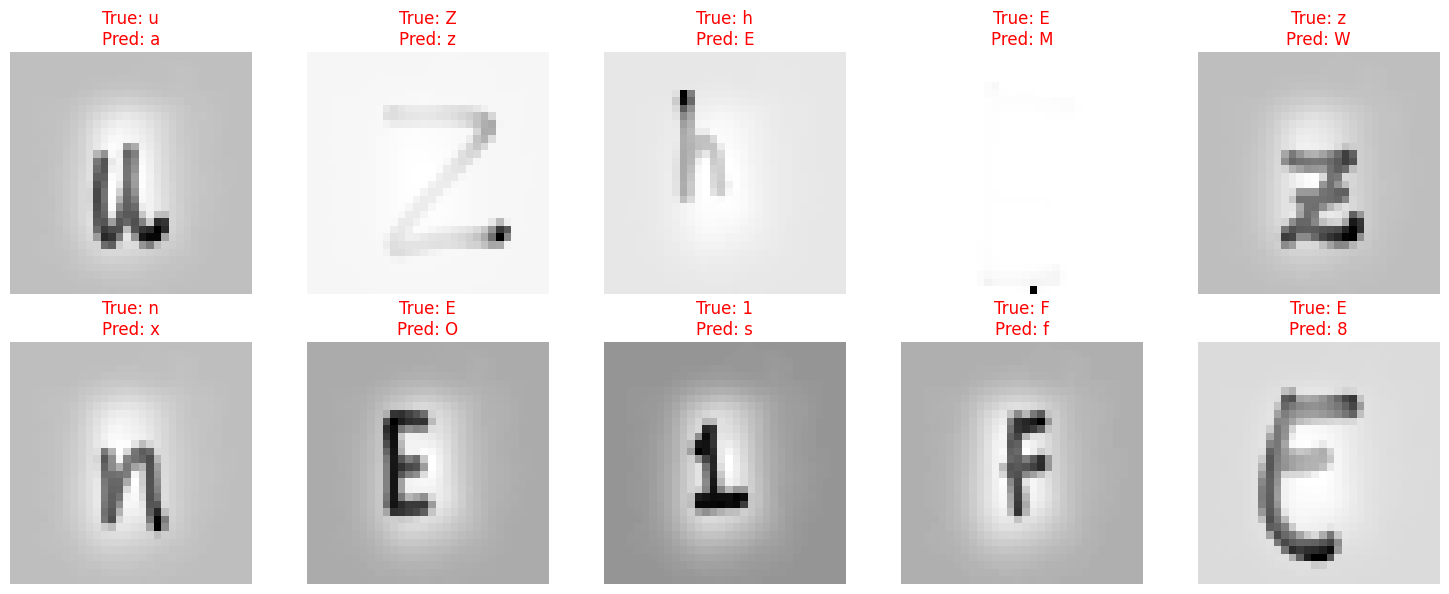
\includegraphics[width=469.5pt,height=192.4658pt]{latexImage_13cf3b8a985fa288314b8d9990a8b50e.png}}
\put(93,-478.7541){\fontsize{21.7728}{1}\usefont{T1}{cmr}{b}{n}\selectfont\color{color_29791}3.MLP Implementation and Results}
\put(93,-512.5625){\fontsize{9.75}{1}\usefont{T1}{cmr}{m}{n}\selectfont\color{color_95391}\# Define MLP model}
\put(93,-525.3126){\fontsize{9.75}{1}\usefont{T1}{cmr}{b}{n}\selectfont\color{color_33759}classMLP(nn.Module):}
\put(116.48,-538.0626){\fontsize{9.75}{1}\usefont{T1}{cmr}{b}{n}\selectfont\color{color_33759}def\_\_init\_\_(self,input\_size,hidden\_sizes,output\_size,activation='relu'}
\put(139.96,-550.8127){\fontsize{9.75}{1}\usefont{T1}{cmr}{m}{n}\selectfont\color{color_62560}super(MLP,self).\_\_init\_\_()}
\put(139.96,-576.3129){\fontsize{9.75}{1}\usefont{T1}{cmr}{m}{n}\selectfont\color{color_95391}\# Create layers}
\put(139.96,-589.0629){\fontsize{9.75}{1}\usefont{T1}{cmr}{m}{n}\selectfont\color{color_62560}layers=[]}
\put(139.96,-601.813){\fontsize{9.75}{1}\usefont{T1}{cmr}{m}{n}\selectfont\color{color_62560}prev\_size=input\_size}
\put(139.96,-627.3132){\fontsize{9.75}{1}\usefont{T1}{cmr}{b}{n}\selectfont\color{color_33759}forhidden\_sizeinhidden\_sizes:}
\put(163.4399,-640.0632){\fontsize{9.75}{1}\usefont{T1}{cmr}{m}{n}\selectfont\color{color_62560}layers.append(nn.Linear(prev\_size,hidden\_size))}
\put(163.4399,-665.5634){\fontsize{9.75}{1}\usefont{T1}{cmr}{m}{n}\selectfont\color{color_95391}\# Add activation function}
\put(163.4399,-678.3135){\fontsize{9.75}{1}\usefont{T1}{cmr}{b}{n}\selectfont\color{color_33759}ifactivation=='relu':}
\put(186.9199,-691.0635){\fontsize{9.75}{1}\usefont{T1}{cmr}{m}{n}\selectfont\color{color_62560}layers.append(nn.ReLU())}
\put(163.4399,-703.8136){\fontsize{9.75}{1}\usefont{T1}{cmr}{b}{n}\selectfont\color{color_33759}elifactivation=='sigmoid':}
\put(186.9199,-716.5637){\fontsize{9.75}{1}\usefont{T1}{cmr}{m}{n}\selectfont\color{color_62560}layers.append(nn.Sigmoid())}
\put(43.66,-512.5625){\fontsize{9.75}{1}\usefont{T1}{cmr}{m}{n}\selectfont\color{color_126112}In[7]:}
\end{picture}
\newpage
\begin{tikzpicture}[overlay]
\path(0pt,0pt);
\filldraw[color_283006][even odd rule]
(21pt, -746pt) -- (561pt, -746pt)
 -- (561pt, -746pt)
 -- (561pt, -26pt)
 -- (561pt, -26pt)
 -- (21pt, -26pt) -- cycle
;
\filldraw[color_273076][even odd rule]
(89.25pt, -722.004pt) -- (549.75pt, -722.004pt)
 -- (549.75pt, -722.004pt)
 -- (549.75pt, -37.25pt)
 -- (549.75pt, -37.25pt)
 -- (89.25pt, -37.25pt) -- cycle
;
\filldraw[color_252223][nonzero rule]
(89.25pt, -722.004pt) -- (90pt, -722.004pt)
 -- (90pt, -722.004pt)
 -- (90pt, -37.25pt)
 -- (90pt, -37.25pt)
 -- (89.25pt, -37.25pt) -- cycle
;
\filldraw[color_252223][nonzero rule]
(549pt, -722.004pt) -- (549.75pt, -722.004pt)
 -- (549.75pt, -722.004pt)
 -- (549.75pt, -37.25pt)
 -- (549.75pt, -37.25pt)
 -- (549pt, -37.25pt) -- cycle
;
\begin{scope}
\clip
(32.25pt, -722.004pt) -- (549.75pt, -722.004pt)
 -- (549.75pt, -722.004pt)
 -- (549.75pt, -37.25pt)
 -- (549.75pt, -37.25pt)
 -- (32.25pt, -37.25pt) -- cycle
;
\begin{scope}
\clip
(90pt, -721.254pt) -- (549pt, -721.254pt)
 -- (549pt, -721.254pt)
 -- (549pt, -38pt)
 -- (549pt, -38pt)
 -- (90pt, -38pt) -- cycle
;
\filldraw[color_273076][even odd rule]
(90pt, -721.254pt) -- (549pt, -721.254pt)
 -- (549pt, -721.254pt)
 -- (549pt, -38pt)
 -- (549pt, -38pt)
 -- (90pt, -38pt) -- cycle
;
\end{scope}
\end{scope}
\begin{scope}
\clip
(32.25pt, -722.004pt) -- (549.75pt, -722.004pt)
 -- (549.75pt, -722.004pt)
 -- (549.75pt, -37.25pt)
 -- (549.75pt, -37.25pt)
 -- (32.25pt, -37.25pt) -- cycle
;
\begin{scope}
\clip
(90pt, -721.254pt) -- (549pt, -721.254pt)
 -- (549pt, -721.254pt)
 -- (549pt, -38pt)
 -- (549pt, -38pt)
 -- (90pt, -38pt) -- cycle
;
\end{scope}
\end{scope}
\end{tikzpicture}
\begin{picture}(-5,0)(2.5,0)
\put(163.4399,-51.50043){\fontsize{9.75}{1}\usefont{T1}{cmr}{b}{n}\selectfont\color{color_33759}elifactivation=='tanh':}
\put(186.9199,-64.25049){\fontsize{9.75}{1}\usefont{T1}{cmr}{m}{n}\selectfont\color{color_62560}layers.append(nn.Tanh())}
\put(163.4399,-89.75061){\fontsize{9.75}{1}\usefont{T1}{cmr}{m}{n}\selectfont\color{color_95391}\# Add dropout for regularization}
\put(163.4399,-102.5007){\fontsize{9.75}{1}\usefont{T1}{cmr}{m}{n}\selectfont\color{color_62560}layers.append(nn.Dropout(dropout\_rate))}
\put(163.4399,-128.0009){\fontsize{9.75}{1}\usefont{T1}{cmr}{m}{n}\selectfont\color{color_62560}prev\_size=hidden\_size}
\put(139.96,-153.501){\fontsize{9.75}{1}\usefont{T1}{cmr}{m}{n}\selectfont\color{color_95391}\# Output layer}
\put(139.96,-166.2511){\fontsize{9.75}{1}\usefont{T1}{cmr}{m}{n}\selectfont\color{color_62560}layers.append(nn.Linear(prev\_size,output\_size))}
\put(139.96,-191.7512){\fontsize{9.75}{1}\usefont{T1}{cmr}{m}{n}\selectfont\color{color_62560}self.model=nn.Sequential(*layers)}
\put(116.48,-217.2514){\fontsize{9.75}{1}\usefont{T1}{cmr}{b}{n}\selectfont\color{color_33759}defforward(self,x):}
\put(139.96,-230.0015){\fontsize{9.75}{1}\usefont{T1}{cmr}{b}{n}\selectfont\color{color_33759}returnself.model(x)}
\put(93,-255.5016){\fontsize{9.75}{1}\usefont{T1}{cmr}{m}{n}\selectfont\color{color_95391}\# Training function with detailed metrics tracking}
\put(93,-268.2517){\fontsize{9.75}{1}\usefont{T1}{cmr}{b}{n}\selectfont\color{color_33759}deftrain\_model(model,train\_loader,val\_loader,criterion,optimizer,num\_epochs}
\put(116.48,-281.0018){\fontsize{9.75}{1}\usefont{T1}{cmr}{m}{n}\selectfont\color{color_62560}train\_losses=[]}
\put(116.48,-293.7518){\fontsize{9.75}{1}\usefont{T1}{cmr}{m}{n}\selectfont\color{color_62560}val\_losses=[]}
\put(116.48,-306.5019){\fontsize{9.75}{1}\usefont{T1}{cmr}{m}{n}\selectfont\color{color_62560}train\_accuracies=[]}
\put(116.48,-319.252){\fontsize{9.75}{1}\usefont{T1}{cmr}{m}{n}\selectfont\color{color_62560}val\_accuracies=[]}
\put(116.48,-344.7521){\fontsize{9.75}{1}\usefont{T1}{cmr}{m}{n}\selectfont\color{color_62560}best\_val\_acc=0.0}
\put(116.48,-357.5022){\fontsize{9.75}{1}\usefont{T1}{cmr}{m}{n}\selectfont\color{color_62560}epochs\_no\_improve=0}
\put(116.48,-370.2523){\fontsize{9.75}{1}\usefont{T1}{cmr}{m}{n}\selectfont\color{color_62560}best\_model\_state=None}
\put(116.48,-395.7524){\fontsize{9.75}{1}\usefont{T1}{cmr}{b}{n}\selectfont\color{color_33759}forepochinrange(num\_epochs):}
\put(139.96,-408.5025){\fontsize{9.75}{1}\usefont{T1}{cmr}{m}{n}\selectfont\color{color_95391}\# Training phase}
\put(139.96,-421.2526){\fontsize{9.75}{1}\usefont{T1}{cmr}{m}{n}\selectfont\color{color_62560}model.train()}
\put(139.96,-434.0027){\fontsize{9.75}{1}\usefont{T1}{cmr}{m}{n}\selectfont\color{color_62560}running\_loss=0.0}
\put(139.96,-446.7527){\fontsize{9.75}{1}\usefont{T1}{cmr}{m}{n}\selectfont\color{color_62560}train\_correct=0}
\put(139.96,-459.5028){\fontsize{9.75}{1}\usefont{T1}{cmr}{m}{n}\selectfont\color{color_62560}train\_total=0}
\put(139.96,-485.003){\fontsize{9.75}{1}\usefont{T1}{cmr}{b}{n}\selectfont\color{color_33759}forinputs,labelsintrain\_loader:}
\put(163.4399,-497.753){\fontsize{9.75}{1}\usefont{T1}{cmr}{m}{n}\selectfont\color{color_62560}optimizer.zero\_grad()}
\put(163.4399,-510.5031){\fontsize{9.75}{1}\usefont{T1}{cmr}{m}{n}\selectfont\color{color_62560}outputs=model(inputs)}
\put(163.4399,-523.2532){\fontsize{9.75}{1}\usefont{T1}{cmr}{m}{n}\selectfont\color{color_62560}loss=criterion(outputs,labels)}
\put(163.4399,-536.0033){\fontsize{9.75}{1}\usefont{T1}{cmr}{m}{n}\selectfont\color{color_62560}loss.backward()}
\put(163.4399,-548.7533){\fontsize{9.75}{1}\usefont{T1}{cmr}{m}{n}\selectfont\color{color_62560}optimizer.step()}
\put(163.4399,-574.2535){\fontsize{9.75}{1}\usefont{T1}{cmr}{m}{n}\selectfont\color{color_62560}running\_loss+=loss.item()*inputs.size(0)}
\put(163.4399,-599.7536){\fontsize{9.75}{1}\usefont{T1}{cmr}{m}{n}\selectfont\color{color_95391}\# Calculate training accuracy}
\put(163.4399,-612.5037){\fontsize{9.75}{1}\usefont{T1}{cmr}{m}{n}\selectfont\color{color_62560}\_,predicted=torch.max(outputs.data,1)}
\put(163.4399,-625.2538){\fontsize{9.75}{1}\usefont{T1}{cmr}{m}{n}\selectfont\color{color_62560}train\_total+=labels.size(0)}
\put(163.4399,-638.0039){\fontsize{9.75}{1}\usefont{T1}{cmr}{m}{n}\selectfont\color{color_62560}train\_correct+=(predicted==labels).sum().item()}
\put(139.96,-663.504){\fontsize{9.75}{1}\usefont{T1}{cmr}{m}{n}\selectfont\color{color_62560}epoch\_train\_loss=running\_loss/len(train\_loader.dataset)}
\put(139.96,-676.2541){\fontsize{9.75}{1}\usefont{T1}{cmr}{m}{n}\selectfont\color{color_62560}epoch\_train\_acc=train\_correct/train\_total}
\put(139.96,-689.0042){\fontsize{9.75}{1}\usefont{T1}{cmr}{m}{n}\selectfont\color{color_62560}train\_losses.append(epoch\_train\_loss)}
\put(139.96,-701.7542){\fontsize{9.75}{1}\usefont{T1}{cmr}{m}{n}\selectfont\color{color_62560}train\_accuracies.append(epoch\_train\_acc)}
\end{picture}
\newpage
\begin{tikzpicture}[overlay]
\path(0pt,0pt);
\filldraw[color_283006][even odd rule]
(21pt, -746pt) -- (561pt, -746pt)
 -- (561pt, -746pt)
 -- (561pt, -26pt)
 -- (561pt, -26pt)
 -- (21pt, -26pt) -- cycle
;
\filldraw[color_273076][even odd rule]
(89.25pt, -722.004pt) -- (549.75pt, -722.004pt)
 -- (549.75pt, -722.004pt)
 -- (549.75pt, -37.25pt)
 -- (549.75pt, -37.25pt)
 -- (89.25pt, -37.25pt) -- cycle
;
\filldraw[color_252223][nonzero rule]
(89.25pt, -722.004pt) -- (90pt, -722.004pt)
 -- (90pt, -722.004pt)
 -- (90pt, -37.25pt)
 -- (90pt, -37.25pt)
 -- (89.25pt, -37.25pt) -- cycle
;
\filldraw[color_252223][nonzero rule]
(549pt, -722.004pt) -- (549.75pt, -722.004pt)
 -- (549.75pt, -722.004pt)
 -- (549.75pt, -37.25pt)
 -- (549.75pt, -37.25pt)
 -- (549pt, -37.25pt) -- cycle
;
\begin{scope}
\clip
(32.25pt, -722.004pt) -- (549.75pt, -722.004pt)
 -- (549.75pt, -722.004pt)
 -- (549.75pt, -37.25pt)
 -- (549.75pt, -37.25pt)
 -- (32.25pt, -37.25pt) -- cycle
;
\begin{scope}
\clip
(90pt, -721.254pt) -- (549pt, -721.254pt)
 -- (549pt, -721.254pt)
 -- (549pt, -38pt)
 -- (549pt, -38pt)
 -- (90pt, -38pt) -- cycle
;
\filldraw[color_273076][even odd rule]
(90pt, -721.254pt) -- (549pt, -721.254pt)
 -- (549pt, -721.254pt)
 -- (549pt, -38pt)
 -- (549pt, -38pt)
 -- (90pt, -38pt) -- cycle
;
\end{scope}
\end{scope}
\begin{scope}
\clip
(32.25pt, -722.004pt) -- (549.75pt, -722.004pt)
 -- (549.75pt, -722.004pt)
 -- (549.75pt, -37.25pt)
 -- (549.75pt, -37.25pt)
 -- (32.25pt, -37.25pt) -- cycle
;
\begin{scope}
\clip
(90pt, -721.254pt) -- (549pt, -721.254pt)
 -- (549pt, -721.254pt)
 -- (549pt, -38pt)
 -- (549pt, -38pt)
 -- (90pt, -38pt) -- cycle
;
\end{scope}
\end{scope}
\end{tikzpicture}
\begin{picture}(-5,0)(2.5,0)
\put(139.96,-51.50043){\fontsize{9.75}{1}\usefont{T1}{cmr}{m}{n}\selectfont\color{color_95391}\# Validation phase}
\put(139.96,-64.25049){\fontsize{9.75}{1}\usefont{T1}{cmr}{m}{n}\selectfont\color{color_62560}model.eval()}
\put(139.96,-77.00061){\fontsize{9.75}{1}\usefont{T1}{cmr}{m}{n}\selectfont\color{color_62560}val\_loss=0.0}
\put(139.96,-89.75061){\fontsize{9.75}{1}\usefont{T1}{cmr}{m}{n}\selectfont\color{color_62560}val\_correct=0}
\put(139.96,-102.5007){\fontsize{9.75}{1}\usefont{T1}{cmr}{m}{n}\selectfont\color{color_62560}val\_total=0}
\put(139.96,-128.0009){\fontsize{9.75}{1}\usefont{T1}{cmr}{b}{n}\selectfont\color{color_33759}withtorch.no\_grad():}
\put(163.4399,-140.7509){\fontsize{9.75}{1}\usefont{T1}{cmr}{b}{n}\selectfont\color{color_33759}forinputs,labelsinval\_loader:}
\put(186.9199,-153.501){\fontsize{9.75}{1}\usefont{T1}{cmr}{m}{n}\selectfont\color{color_62560}outputs=model(inputs)}
\put(186.9199,-166.2511){\fontsize{9.75}{1}\usefont{T1}{cmr}{m}{n}\selectfont\color{color_62560}loss=criterion(outputs,labels)}
\put(186.9199,-179.0012){\fontsize{9.75}{1}\usefont{T1}{cmr}{m}{n}\selectfont\color{color_62560}val\_loss+=loss.item()*inputs.size(0)}
\put(186.9199,-204.5013){\fontsize{9.75}{1}\usefont{T1}{cmr}{m}{n}\selectfont\color{color_62560}\_,predicted=torch.max(outputs.data,1)}
\put(186.9199,-217.2514){\fontsize{9.75}{1}\usefont{T1}{cmr}{m}{n}\selectfont\color{color_62560}val\_total+=labels.size(0)}
\put(186.9199,-230.0015){\fontsize{9.75}{1}\usefont{T1}{cmr}{m}{n}\selectfont\color{color_62560}val\_correct+=(predicted==labels).sum().item()}
\put(139.96,-255.5016){\fontsize{9.75}{1}\usefont{T1}{cmr}{m}{n}\selectfont\color{color_62560}epoch\_val\_loss=val\_loss/len(val\_loader.dataset)}
\put(139.96,-268.2517){\fontsize{9.75}{1}\usefont{T1}{cmr}{m}{n}\selectfont\color{color_62560}epoch\_val\_acc=val\_correct/val\_total}
\put(139.96,-281.0018){\fontsize{9.75}{1}\usefont{T1}{cmr}{m}{n}\selectfont\color{color_62560}val\_losses.append(epoch\_val\_loss)}
\put(139.96,-293.7518){\fontsize{9.75}{1}\usefont{T1}{cmr}{m}{n}\selectfont\color{color_62560}val\_accuracies.append(epoch\_val\_acc)}
\put(139.96,-319.252){\fontsize{9.75}{1}\usefont{T1}{cmr}{m}{n}\selectfont\color{color_95391}\# Check for improvement}
\put(139.96,-332.0021){\fontsize{9.75}{1}\usefont{T1}{cmr}{b}{n}\selectfont\color{color_33759}ifepoch\_val\_acc>best\_val\_acc:}
\put(163.4399,-344.7521){\fontsize{9.75}{1}\usefont{T1}{cmr}{m}{n}\selectfont\color{color_62560}best\_val\_acc=epoch\_val\_acc}
\put(163.4399,-357.5022){\fontsize{9.75}{1}\usefont{T1}{cmr}{m}{n}\selectfont\color{color_62560}best\_model\_state=model.state\_dict().copy()}
\put(163.4399,-370.2523){\fontsize{9.75}{1}\usefont{T1}{cmr}{m}{n}\selectfont\color{color_62560}epochs\_no\_improve=0}
\put(139.96,-383.0024){\fontsize{9.75}{1}\usefont{T1}{cmr}{b}{n}\selectfont\color{color_33759}else:}
\put(163.4399,-395.7524){\fontsize{9.75}{1}\usefont{T1}{cmr}{m}{n}\selectfont\color{color_62560}epochs\_no\_improve+=1}
\put(139.96,-421.2526){\fontsize{9.75}{1}\usefont{T1}{cmr}{m}{n}\selectfont\color{color_95391}\# Early stopping}
\put(139.96,-434.0027){\fontsize{9.75}{1}\usefont{T1}{cmr}{b}{n}\selectfont\color{color_33759}ifepochs\_no\_improve>=patience:}
\put(163.4399,-446.7527){\fontsize{9.75}{1}\usefont{T1}{cmr}{m}{n}\selectfont\color{color_62560}print(f"Early stopping at epoch\{epoch+1\}")}
\put(163.4399,-459.5028){\fontsize{9.75}{1}\usefont{T1}{cmr}{b}{n}\selectfont\color{color_33759}break}
\put(139.96,-485.003){\fontsize{9.75}{1}\usefont{T1}{cmr}{b}{n}\selectfont\color{color_33759}if(epoch+1)\%10==0:}
\put(163.4399,-497.753){\fontsize{9.75}{1}\usefont{T1}{cmr}{m}{n}\selectfont\color{color_62560}print(f"Epoch\{epoch+1\}/\{num\_epochs\}, Train Loss:\{epoch\_train\_loss}
\put(163.4399,-510.5031){\fontsize{9.75}{1}\usefont{T1}{cmr}{m}{n}\selectfont\color{color_62560}print(f"Train Acc:\{epoch\_train\_acc:.4f\}, Val Acc:\{epoch\_val\_acc:.4f}
\put(116.48,-536.0033){\fontsize{9.75}{1}\usefont{T1}{cmr}{m}{n}\selectfont\color{color_95391}\# Load best model}
\put(116.48,-548.7533){\fontsize{9.75}{1}\usefont{T1}{cmr}{b}{n}\selectfont\color{color_33759}ifbest\_model\_stateisnotNone:}
\put(139.96,-561.5034){\fontsize{9.75}{1}\usefont{T1}{cmr}{m}{n}\selectfont\color{color_62560}model.load\_state\_dict(best\_model\_state)}
\put(116.48,-587.0036){\fontsize{9.75}{1}\usefont{T1}{cmr}{b}{n}\selectfont\color{color_33759}returnmodel,train\_losses,val\_losses,train\_accuracies,val\_accuracies}
\put(93,-612.5037){\fontsize{9.75}{1}\usefont{T1}{cmr}{m}{n}\selectfont\color{color_95391}\# Evaluation function with probability outputs}
\put(93,-625.2538){\fontsize{9.75}{1}\usefont{T1}{cmr}{b}{n}\selectfont\color{color_33759}defevaluate\_model(model,test\_loader):}
\put(116.48,-638.0039){\fontsize{9.75}{1}\usefont{T1}{cmr}{m}{n}\selectfont\color{color_62560}model.eval()}
\put(116.48,-650.7539){\fontsize{9.75}{1}\usefont{T1}{cmr}{m}{n}\selectfont\color{color_62560}correct=0}
\put(116.48,-663.504){\fontsize{9.75}{1}\usefont{T1}{cmr}{m}{n}\selectfont\color{color_62560}total=0}
\put(116.48,-676.2541){\fontsize{9.75}{1}\usefont{T1}{cmr}{m}{n}\selectfont\color{color_62560}all\_preds=[]}
\put(116.48,-689.0042){\fontsize{9.75}{1}\usefont{T1}{cmr}{m}{n}\selectfont\color{color_62560}all\_labels=[]}
\put(116.48,-701.7542){\fontsize{9.75}{1}\usefont{T1}{cmr}{m}{n}\selectfont\color{color_62560}all\_probs=[]}
\end{picture}
\newpage
\begin{tikzpicture}[overlay]
\path(0pt,0pt);
\filldraw[color_283006][even odd rule]
(21pt, -746pt) -- (561pt, -746pt)
 -- (561pt, -746pt)
 -- (561pt, -26pt)
 -- (561pt, -26pt)
 -- (21pt, -26pt) -- cycle
;
\filldraw[color_273076][even odd rule]
(89.25pt, -722.004pt) -- (549.75pt, -722.004pt)
 -- (549.75pt, -722.004pt)
 -- (549.75pt, -37.25pt)
 -- (549.75pt, -37.25pt)
 -- (89.25pt, -37.25pt) -- cycle
;
\filldraw[color_252223][nonzero rule]
(89.25pt, -722.004pt) -- (90pt, -722.004pt)
 -- (90pt, -722.004pt)
 -- (90pt, -37.25pt)
 -- (90pt, -37.25pt)
 -- (89.25pt, -37.25pt) -- cycle
;
\filldraw[color_252223][nonzero rule]
(549pt, -722.004pt) -- (549.75pt, -722.004pt)
 -- (549.75pt, -722.004pt)
 -- (549.75pt, -37.25pt)
 -- (549.75pt, -37.25pt)
 -- (549pt, -37.25pt) -- cycle
;
\begin{scope}
\clip
(32.25pt, -722.004pt) -- (549.75pt, -722.004pt)
 -- (549.75pt, -722.004pt)
 -- (549.75pt, -37.25pt)
 -- (549.75pt, -37.25pt)
 -- (32.25pt, -37.25pt) -- cycle
;
\begin{scope}
\clip
(90pt, -721.254pt) -- (549pt, -721.254pt)
 -- (549pt, -721.254pt)
 -- (549pt, -38pt)
 -- (549pt, -38pt)
 -- (90pt, -38pt) -- cycle
;
\filldraw[color_273076][even odd rule]
(90pt, -721.254pt) -- (549pt, -721.254pt)
 -- (549pt, -721.254pt)
 -- (549pt, -38pt)
 -- (549pt, -38pt)
 -- (90pt, -38pt) -- cycle
;
\end{scope}
\end{scope}
\begin{scope}
\clip
(32.25pt, -722.004pt) -- (549.75pt, -722.004pt)
 -- (549.75pt, -722.004pt)
 -- (549.75pt, -37.25pt)
 -- (549.75pt, -37.25pt)
 -- (32.25pt, -37.25pt) -- cycle
;
\begin{scope}
\clip
(90pt, -721.254pt) -- (549pt, -721.254pt)
 -- (549pt, -721.254pt)
 -- (549pt, -38pt)
 -- (549pt, -38pt)
 -- (90pt, -38pt) -- cycle
;
\end{scope}
\end{scope}
\end{tikzpicture}
\begin{picture}(-5,0)(2.5,0)
\put(116.48,-51.50043){\fontsize{9.75}{1}\usefont{T1}{cmr}{b}{n}\selectfont\color{color_33759}withtorch.no\_grad():}
\put(139.96,-64.25049){\fontsize{9.75}{1}\usefont{T1}{cmr}{b}{n}\selectfont\color{color_33759}forinputs,labelsintest\_loader:}
\put(163.4399,-77.00061){\fontsize{9.75}{1}\usefont{T1}{cmr}{m}{n}\selectfont\color{color_62560}outputs=model(inputs)}
\put(163.4399,-89.75061){\fontsize{9.75}{1}\usefont{T1}{cmr}{m}{n}\selectfont\color{color_62560}probs=torch.softmax(outputs,dim=1)}
\put(163.4399,-102.5007){\fontsize{9.75}{1}\usefont{T1}{cmr}{m}{n}\selectfont\color{color_62560}\_,predicted=torch.max(outputs.data,1)}
\put(163.4399,-115.2508){\fontsize{9.75}{1}\usefont{T1}{cmr}{m}{n}\selectfont\color{color_62560}total+=labels.size(0)}
\put(163.4399,-128.0009){\fontsize{9.75}{1}\usefont{T1}{cmr}{m}{n}\selectfont\color{color_62560}correct+=(predicted==labels).sum().item()}
\put(163.4399,-153.501){\fontsize{9.75}{1}\usefont{T1}{cmr}{m}{n}\selectfont\color{color_62560}all\_preds.extend(predicted.cpu().numpy())}
\put(163.4399,-166.2511){\fontsize{9.75}{1}\usefont{T1}{cmr}{m}{n}\selectfont\color{color_62560}all\_labels.extend(labels.cpu().numpy())}
\put(163.4399,-179.0012){\fontsize{9.75}{1}\usefont{T1}{cmr}{m}{n}\selectfont\color{color_62560}all\_probs.extend(probs.cpu().numpy())}
\put(116.48,-204.5013){\fontsize{9.75}{1}\usefont{T1}{cmr}{m}{n}\selectfont\color{color_62560}accuracy=correct/total}
\put(116.48,-217.2514){\fontsize{9.75}{1}\usefont{T1}{cmr}{b}{n}\selectfont\color{color_33759}returnaccuracy,np.array(all\_preds),np.array(all\_labels),np.array(all\_probs}
\put(93,-242.7515){\fontsize{9.75}{1}\usefont{T1}{cmr}{m}{n}\selectfont\color{color_95391}\# --- IMPORTANT: ensure DataLoaders exist (this is the minimal required fix) ---}
\put(93,-255.5016){\fontsize{9.75}{1}\usefont{T1}{cmr}{m}{n}\selectfont\color{color_95391}\# You already created train\_dataset, val\_dataset, test\_dataset earlier.}
\put(93,-268.2517){\fontsize{9.75}{1}\usefont{T1}{cmr}{m}{n}\selectfont\color{color_95391}\# Create matching DataLoader objects expected by the training/eval code:}
\put(93,-293.7518){\fontsize{9.75}{1}\usefont{T1}{cmr}{m}{n}\selectfont\color{color_62560}batch\_size=64\# adjust if you want}
\put(93,-306.5019){\fontsize{9.75}{1}\usefont{T1}{cmr}{m}{n}\selectfont\color{color_62560}train\_loader=DataLoader(train\_dataset,batch\_size=batch\_size,shuffle=True)}
\put(93,-319.252){\fontsize{9.75}{1}\usefont{T1}{cmr}{m}{n}\selectfont\color{color_62560}val\_loader=DataLoader(val\_dataset,batch\_size=batch\_size,shuffle=False)}
\put(93,-332.0021){\fontsize{9.75}{1}\usefont{T1}{cmr}{m}{n}\selectfont\color{color_62560}test\_loader=DataLoader(test\_dataset,batch\_size=batch\_size,shuffle=False)}
\put(93,-357.5022){\fontsize{9.75}{1}\usefont{T1}{cmr}{m}{n}\selectfont\color{color_95391}\# Hyperparameter tuning}
\put(93,-370.2523){\fontsize{9.75}{1}\usefont{T1}{cmr}{m}{n}\selectfont\color{color_62560}hidden\_layers\_options=[[128],[256],[128,64],[256,128]]}
\put(93,-383.0024){\fontsize{9.75}{1}\usefont{T1}{cmr}{m}{n}\selectfont\color{color_62560}activation\_options=['relu','sigmoid','tanh']}
\put(93,-395.7524){\fontsize{9.75}{1}\usefont{T1}{cmr}{m}{n}\selectfont\color{color_62560}learning\_rates=[0.001,0.01,0.1]}
\put(93,-408.5025){\fontsize{9.75}{1}\usefont{T1}{cmr}{m}{n}\selectfont\color{color_62560}optimizers\_list=['adam','sgd']}
\put(93,-434.0027){\fontsize{9.75}{1}\usefont{T1}{cmr}{m}{n}\selectfont\color{color_95391}\# Tuning loop}
\put(93,-446.7527){\fontsize{9.75}{1}\usefont{T1}{cmr}{m}{n}\selectfont\color{color_62560}best\_val\_acc=0}
\put(93,-459.5028){\fontsize{9.75}{1}\usefont{T1}{cmr}{m}{n}\selectfont\color{color_62560}best\_params=\{\}}
\put(93,-472.2529){\fontsize{9.75}{1}\usefont{T1}{cmr}{m}{n}\selectfont\color{color_62560}best\_model=None}
\put(93,-485.003){\fontsize{9.75}{1}\usefont{T1}{cmr}{m}{n}\selectfont\color{color_62560}all\_results=[]}
\put(93,-510.5031){\fontsize{9.75}{1}\usefont{T1}{cmr}{m}{n}\selectfont\color{color_62560}print("Starting hyperparameter tuning...")}
\put(93,-536.0033){\fontsize{9.75}{1}\usefont{T1}{cmr}{m}{n}\selectfont\color{color_62560}input\_size=X\_train.shape[1]}
\put(93,-548.7533){\fontsize{9.75}{1}\usefont{T1}{cmr}{m}{n}\selectfont\color{color_62560}num\_classes=len(np.unique(y\_train))}
\put(93,-574.2535){\fontsize{9.75}{1}\usefont{T1}{cmr}{b}{n}\selectfont\color{color_33759}forhidden\_layersinhidden\_layers\_options:}
\put(116.48,-587.0036){\fontsize{9.75}{1}\usefont{T1}{cmr}{b}{n}\selectfont\color{color_33759}foractivationinactivation\_options:}
\put(139.96,-599.7536){\fontsize{9.75}{1}\usefont{T1}{cmr}{b}{n}\selectfont\color{color_33759}forlrinlearning\_rates:}
\put(163.4399,-612.5037){\fontsize{9.75}{1}\usefont{T1}{cmr}{b}{n}\selectfont\color{color_33759}foropt\_nameinoptimizers\_list:}
\put(186.9199,-625.2538){\fontsize{9.75}{1}\usefont{T1}{cmr}{m}{n}\selectfont\color{color_62560}print(f"Testing: Layers=\{hidden\_layers\}, Activation=\{activation}
\put(186.9199,-650.7539){\fontsize{9.75}{1}\usefont{T1}{cmr}{m}{n}\selectfont\color{color_95391}\# Initialize model}
\put(186.9199,-663.504){\fontsize{9.75}{1}\usefont{T1}{cmr}{m}{n}\selectfont\color{color_62560}model=MLP(input\_size,hidden\_layers,num\_classes,activation=}
\put(186.9199,-689.0042){\fontsize{9.75}{1}\usefont{T1}{cmr}{m}{n}\selectfont\color{color_95391}\# Define loss and optimizer}
\put(186.9199,-701.7542){\fontsize{9.75}{1}\usefont{T1}{cmr}{m}{n}\selectfont\color{color_62560}criterion=nn.CrossEntropyLoss()}
\end{picture}
\newpage
\begin{tikzpicture}[overlay]
\path(0pt,0pt);
\filldraw[color_283006][even odd rule]
(21pt, -746pt) -- (561pt, -746pt)
 -- (561pt, -746pt)
 -- (561pt, -26pt)
 -- (561pt, -26pt)
 -- (21pt, -26pt) -- cycle
;
\filldraw[color_273076][even odd rule]
(89.25pt, -722.004pt) -- (549.75pt, -722.004pt)
 -- (549.75pt, -722.004pt)
 -- (549.75pt, -37.25pt)
 -- (549.75pt, -37.25pt)
 -- (89.25pt, -37.25pt) -- cycle
;
\filldraw[color_252223][nonzero rule]
(89.25pt, -722.004pt) -- (90pt, -722.004pt)
 -- (90pt, -722.004pt)
 -- (90pt, -37.25pt)
 -- (90pt, -37.25pt)
 -- (89.25pt, -37.25pt) -- cycle
;
\filldraw[color_252223][nonzero rule]
(549pt, -722.004pt) -- (549.75pt, -722.004pt)
 -- (549.75pt, -722.004pt)
 -- (549.75pt, -37.25pt)
 -- (549.75pt, -37.25pt)
 -- (549pt, -37.25pt) -- cycle
;
\begin{scope}
\clip
(32.25pt, -722.004pt) -- (549.75pt, -722.004pt)
 -- (549.75pt, -722.004pt)
 -- (549.75pt, -37.25pt)
 -- (549.75pt, -37.25pt)
 -- (32.25pt, -37.25pt) -- cycle
;
\begin{scope}
\clip
(90pt, -721.254pt) -- (549pt, -721.254pt)
 -- (549pt, -721.254pt)
 -- (549pt, -38pt)
 -- (549pt, -38pt)
 -- (90pt, -38pt) -- cycle
;
\filldraw[color_273076][even odd rule]
(90pt, -721.254pt) -- (549pt, -721.254pt)
 -- (549pt, -721.254pt)
 -- (549pt, -38pt)
 -- (549pt, -38pt)
 -- (90pt, -38pt) -- cycle
;
\end{scope}
\end{scope}
\begin{scope}
\clip
(32.25pt, -722.004pt) -- (549.75pt, -722.004pt)
 -- (549.75pt, -722.004pt)
 -- (549.75pt, -37.25pt)
 -- (549.75pt, -37.25pt)
 -- (32.25pt, -37.25pt) -- cycle
;
\begin{scope}
\clip
(90pt, -721.254pt) -- (549pt, -721.254pt)
 -- (549pt, -721.254pt)
 -- (549pt, -38pt)
 -- (549pt, -38pt)
 -- (90pt, -38pt) -- cycle
;
\end{scope}
\end{scope}
\end{tikzpicture}
\begin{picture}(-5,0)(2.5,0)
\put(186.9199,-51.50043){\fontsize{9.75}{1}\usefont{T1}{cmr}{b}{n}\selectfont\color{color_33759}ifopt\_name=='adam':}
\put(210.3999,-64.25049){\fontsize{9.75}{1}\usefont{T1}{cmr}{m}{n}\selectfont\color{color_62560}optimizer=optim.Adam(model.parameters(),lr=lr)}
\put(186.9199,-77.00061){\fontsize{9.75}{1}\usefont{T1}{cmr}{b}{n}\selectfont\color{color_33759}else:}
\put(210.3999,-89.75061){\fontsize{9.75}{1}\usefont{T1}{cmr}{m}{n}\selectfont\color{color_62560}optimizer=optim.SGD(model.parameters(),lr=lr,momentum=0.9}
\put(186.9199,-115.2508){\fontsize{9.75}{1}\usefont{T1}{cmr}{m}{n}\selectfont\color{color_95391}\# Train model}
\put(186.9199,-128.0009){\fontsize{9.75}{1}\usefont{T1}{cmr}{m}{n}\selectfont\color{color_62560}model,train\_losses,val\_losses,train\_accs,val\_accs=train\_model}
\put(210.3999,-140.7509){\fontsize{9.75}{1}\usefont{T1}{cmr}{m}{n}\selectfont\color{color_62560}model,train\_loader,val\_loader,criterion,optimizer,}
\put(210.3999,-153.501){\fontsize{9.75}{1}\usefont{T1}{cmr}{m}{n}\selectfont\color{color_62560}num\_epochs=50,patience=7}
\put(186.9199,-166.2511){\fontsize{9.75}{1}\usefont{T1}{cmr}{m}{n}\selectfont\color{color_32596})}
\put(186.9199,-191.7512){\fontsize{9.75}{1}\usefont{T1}{cmr}{m}{n}\selectfont\color{color_95391}\# Evaluate on validation set}
\put(186.9199,-204.5013){\fontsize{9.75}{1}\usefont{T1}{cmr}{m}{n}\selectfont\color{color_62560}val\_acc,\_,\_,\_=evaluate\_model(model,val\_loader)}
\put(186.9199,-230.0015){\fontsize{9.75}{1}\usefont{T1}{cmr}{m}{n}\selectfont\color{color_62560}print(f"Validation Accuracy:\{val\_acc:.4f\}")}
\put(186.9199,-255.5016){\fontsize{9.75}{1}\usefont{T1}{cmr}{m}{n}\selectfont\color{color_95391}\# Store results}
\put(186.9199,-268.2517){\fontsize{9.75}{1}\usefont{T1}{cmr}{m}{n}\selectfont\color{color_62560}result=\{}
\put(210.3999,-281.0018){\fontsize{9.75}{1}\usefont{T1}{cmr}{m}{n}\selectfont\color{color_209593}'hidden\_layers':hidden\_layers,}
\put(210.3999,-293.7518){\fontsize{9.75}{1}\usefont{T1}{cmr}{m}{n}\selectfont\color{color_209593}'activation':activation,}
\put(210.3999,-306.5019){\fontsize{9.75}{1}\usefont{T1}{cmr}{m}{n}\selectfont\color{color_209593}'learning\_rate':lr,}
\put(210.3999,-319.252){\fontsize{9.75}{1}\usefont{T1}{cmr}{m}{n}\selectfont\color{color_209593}'optimizer':opt\_name,}
\put(210.3999,-332.0021){\fontsize{9.75}{1}\usefont{T1}{cmr}{m}{n}\selectfont\color{color_209593}'val\_accuracy':val\_acc,}
\put(210.3999,-344.7521){\fontsize{9.75}{1}\usefont{T1}{cmr}{m}{n}\selectfont\color{color_209593}'train\_losses':train\_losses,}
\put(210.3999,-357.5022){\fontsize{9.75}{1}\usefont{T1}{cmr}{m}{n}\selectfont\color{color_209593}'val\_losses':val\_losses,}
\put(210.3999,-370.2523){\fontsize{9.75}{1}\usefont{T1}{cmr}{m}{n}\selectfont\color{color_209593}'train\_accs':train\_accs,}
\put(210.3999,-383.0024){\fontsize{9.75}{1}\usefont{T1}{cmr}{m}{n}\selectfont\color{color_209593}'val\_accs':val\_accs}
\put(186.9199,-395.7524){\fontsize{9.75}{1}\usefont{T1}{cmr}{m}{n}\selectfont\color{color_32596}\}}
\put(186.9199,-408.5025){\fontsize{9.75}{1}\usefont{T1}{cmr}{m}{n}\selectfont\color{color_62560}all\_results.append(result)}
\put(186.9199,-434.0027){\fontsize{9.75}{1}\usefont{T1}{cmr}{m}{n}\selectfont\color{color_95391}\# Update best model}
\put(186.9199,-446.7527){\fontsize{9.75}{1}\usefont{T1}{cmr}{b}{n}\selectfont\color{color_33759}ifval\_acc>best\_val\_acc:}
\put(210.3999,-459.5028){\fontsize{9.75}{1}\usefont{T1}{cmr}{m}{n}\selectfont\color{color_62560}best\_val\_acc=val\_acc}
\put(210.3999,-472.2529){\fontsize{9.75}{1}\usefont{T1}{cmr}{m}{n}\selectfont\color{color_62560}best\_params=\{}
\put(233.8799,-485.003){\fontsize{9.75}{1}\usefont{T1}{cmr}{m}{n}\selectfont\color{color_209593}'hidden\_layers':hidden\_layers,}
\put(233.8799,-497.753){\fontsize{9.75}{1}\usefont{T1}{cmr}{m}{n}\selectfont\color{color_209593}'activation':activation,}
\put(233.8799,-510.5031){\fontsize{9.75}{1}\usefont{T1}{cmr}{m}{n}\selectfont\color{color_209593}'learning\_rate':lr,}
\put(233.8799,-523.2532){\fontsize{9.75}{1}\usefont{T1}{cmr}{m}{n}\selectfont\color{color_209593}'optimizer':opt\_name}
\put(210.3999,-536.0033){\fontsize{9.75}{1}\usefont{T1}{cmr}{m}{n}\selectfont\color{color_32596}\}}
\put(210.3999,-548.7533){\fontsize{9.75}{1}\usefont{T1}{cmr}{m}{n}\selectfont\color{color_62560}best\_model=model}
\put(210.3999,-561.5034){\fontsize{9.75}{1}\usefont{T1}{cmr}{m}{n}\selectfont\color{color_62560}print("New best model found!")}
\put(93,-587.0036){\fontsize{9.75}{1}\usefont{T1}{cmr}{m}{n}\selectfont\color{color_62560}print("Tuning completed!")}
\put(93,-599.7536){\fontsize{9.75}{1}\usefont{T1}{cmr}{m}{n}\selectfont\color{color_62560}print(f"Best validation accuracy:\{best\_val\_acc:.4f\}")}
\put(93,-612.5037){\fontsize{9.75}{1}\usefont{T1}{cmr}{m}{n}\selectfont\color{color_62560}print(f"Best parameters:\{best\_params\}")}
\put(93,-638.0039){\fontsize{9.75}{1}\usefont{T1}{cmr}{m}{n}\selectfont\color{color_95391}\# Plot training curves for all configurations}
\put(93,-650.7539){\fontsize{9.75}{1}\usefont{T1}{cmr}{m}{n}\selectfont\color{color_62560}fig,axes=plt.subplots(2,2,figsize=(15,12))}
\put(93,-663.504){\fontsize{9.75}{1}\usefont{T1}{cmr}{m}{n}\selectfont\color{color_62560}axes=axes.flatten()}
\put(93,-689.0042){\fontsize{9.75}{1}\usefont{T1}{cmr}{b}{n}\selectfont\color{color_33759}fori,resultinenumerate(all\_results):}
\put(116.48,-701.7542){\fontsize{9.75}{1}\usefont{T1}{cmr}{m}{n}\selectfont\color{color_62560}axes[0].plot(result['train\_losses'],label=f"Config\{i+1\}")}
\put(116.48,-714.5043){\fontsize{9.75}{1}\usefont{T1}{cmr}{m}{n}\selectfont\color{color_62560}axes[1].plot(result['val\_losses'],label=f"Config\{i+1\}")}
\end{picture}
\newpage
\begin{tikzpicture}[overlay]
\path(0pt,0pt);
\filldraw[color_283006][even odd rule]
(21pt, -746pt) -- (561pt, -746pt)
 -- (561pt, -746pt)
 -- (561pt, -26pt)
 -- (561pt, -26pt)
 -- (21pt, -26pt) -- cycle
;
\filldraw[color_273076][even odd rule]
(89.25pt, -722.004pt) -- (549.75pt, -722.004pt)
 -- (549.75pt, -722.004pt)
 -- (549.75pt, -37.25pt)
 -- (549.75pt, -37.25pt)
 -- (89.25pt, -37.25pt) -- cycle
;
\filldraw[color_252223][nonzero rule]
(89.25pt, -722.004pt) -- (90pt, -722.004pt)
 -- (90pt, -722.004pt)
 -- (90pt, -37.25pt)
 -- (90pt, -37.25pt)
 -- (89.25pt, -37.25pt) -- cycle
;
\filldraw[color_252223][nonzero rule]
(549pt, -722.004pt) -- (549.75pt, -722.004pt)
 -- (549.75pt, -722.004pt)
 -- (549.75pt, -37.25pt)
 -- (549.75pt, -37.25pt)
 -- (549pt, -37.25pt) -- cycle
;
\begin{scope}
\clip
(32.25pt, -722.004pt) -- (549.75pt, -722.004pt)
 -- (549.75pt, -722.004pt)
 -- (549.75pt, -37.25pt)
 -- (549.75pt, -37.25pt)
 -- (32.25pt, -37.25pt) -- cycle
;
\begin{scope}
\clip
(90pt, -721.254pt) -- (549pt, -721.254pt)
 -- (549pt, -721.254pt)
 -- (549pt, -38pt)
 -- (549pt, -38pt)
 -- (90pt, -38pt) -- cycle
;
\filldraw[color_273076][even odd rule]
(90pt, -721.254pt) -- (549pt, -721.254pt)
 -- (549pt, -721.254pt)
 -- (549pt, -38pt)
 -- (549pt, -38pt)
 -- (90pt, -38pt) -- cycle
;
\end{scope}
\end{scope}
\begin{scope}
\clip
(32.25pt, -722.004pt) -- (549.75pt, -722.004pt)
 -- (549.75pt, -722.004pt)
 -- (549.75pt, -37.25pt)
 -- (549.75pt, -37.25pt)
 -- (32.25pt, -37.25pt) -- cycle
;
\begin{scope}
\clip
(90pt, -721.254pt) -- (549pt, -721.254pt)
 -- (549pt, -721.254pt)
 -- (549pt, -38pt)
 -- (549pt, -38pt)
 -- (90pt, -38pt) -- cycle
;
\end{scope}
\end{scope}
\end{tikzpicture}
\begin{picture}(-5,0)(2.5,0)
\put(116.48,-51.50043){\fontsize{9.75}{1}\usefont{T1}{cmr}{m}{n}\selectfont\color{color_62560}axes[2].plot(result['train\_accs'],label=f"Config\{i+1\}")}
\put(116.48,-64.25049){\fontsize{9.75}{1}\usefont{T1}{cmr}{m}{n}\selectfont\color{color_62560}axes[3].plot(result['val\_accs'],label=f"Config\{i+1\}")}
\put(93,-89.75061){\fontsize{9.75}{1}\usefont{T1}{cmr}{m}{n}\selectfont\color{color_62560}axes[0].set\_title('Training Loss')}
\put(93,-102.5007){\fontsize{9.75}{1}\usefont{T1}{cmr}{m}{n}\selectfont\color{color_62560}axes[0].set\_xlabel('Epoch')}
\put(93,-115.2508){\fontsize{9.75}{1}\usefont{T1}{cmr}{m}{n}\selectfont\color{color_62560}axes[0].set\_ylabel('Loss')}
\put(93,-128.0009){\fontsize{9.75}{1}\usefont{T1}{cmr}{m}{n}\selectfont\color{color_62560}axes[0].legend()}
\put(93,-153.501){\fontsize{9.75}{1}\usefont{T1}{cmr}{m}{n}\selectfont\color{color_62560}axes[1].set\_title('Validation Loss')}
\put(93,-166.2511){\fontsize{9.75}{1}\usefont{T1}{cmr}{m}{n}\selectfont\color{color_62560}axes[1].set\_xlabel('Epoch')}
\put(93,-179.0012){\fontsize{9.75}{1}\usefont{T1}{cmr}{m}{n}\selectfont\color{color_62560}axes[1].set\_ylabel('Loss')}
\put(93,-191.7512){\fontsize{9.75}{1}\usefont{T1}{cmr}{m}{n}\selectfont\color{color_62560}axes[1].legend()}
\put(93,-217.2514){\fontsize{9.75}{1}\usefont{T1}{cmr}{m}{n}\selectfont\color{color_62560}axes[2].set\_title('Training Accuracy')}
\put(93,-230.0015){\fontsize{9.75}{1}\usefont{T1}{cmr}{m}{n}\selectfont\color{color_62560}axes[2].set\_xlabel('Epoch')}
\put(93,-242.7515){\fontsize{9.75}{1}\usefont{T1}{cmr}{m}{n}\selectfont\color{color_62560}axes[2].set\_ylabel('Accuracy')}
\put(93,-255.5016){\fontsize{9.75}{1}\usefont{T1}{cmr}{m}{n}\selectfont\color{color_62560}axes[2].legend()}
\put(93,-281.0018){\fontsize{9.75}{1}\usefont{T1}{cmr}{m}{n}\selectfont\color{color_62560}axes[3].set\_title('Validation Accuracy')}
\put(93,-293.7518){\fontsize{9.75}{1}\usefont{T1}{cmr}{m}{n}\selectfont\color{color_62560}axes[3].set\_xlabel('Epoch')}
\put(93,-306.5019){\fontsize{9.75}{1}\usefont{T1}{cmr}{m}{n}\selectfont\color{color_62560}axes[3].set\_ylabel('Accuracy')}
\put(93,-319.252){\fontsize{9.75}{1}\usefont{T1}{cmr}{m}{n}\selectfont\color{color_62560}axes[3].legend()}
\put(93,-344.7521){\fontsize{9.75}{1}\usefont{T1}{cmr}{m}{n}\selectfont\color{color_62560}plt.tight\_layout()}
\put(93,-357.5022){\fontsize{9.75}{1}\usefont{T1}{cmr}{m}{n}\selectfont\color{color_62560}plt.show()}
\put(93,-383.0024){\fontsize{9.75}{1}\usefont{T1}{cmr}{m}{n}\selectfont\color{color_95391}\# Train the best model with more epochs}
\put(93,-395.7524){\fontsize{9.75}{1}\usefont{T1}{cmr}{m}{n}\selectfont\color{color_62560}print("Training best model with optimal parameters...")}
\put(93,-421.2526){\fontsize{9.75}{1}\usefont{T1}{cmr}{m}{n}\selectfont\color{color_95391}\# Reinitialize best model with best parameters}
\put(93,-434.0027){\fontsize{9.75}{1}\usefont{T1}{cmr}{m}{n}\selectfont\color{color_62560}final\_model=MLP(}
\put(116.48,-446.7527){\fontsize{9.75}{1}\usefont{T1}{cmr}{m}{n}\selectfont\color{color_62560}input\_size,}
\put(116.48,-459.5028){\fontsize{9.75}{1}\usefont{T1}{cmr}{m}{n}\selectfont\color{color_62560}best\_params['hidden\_layers'],}
\put(116.48,-472.2529){\fontsize{9.75}{1}\usefont{T1}{cmr}{m}{n}\selectfont\color{color_62560}num\_classes,}
\put(116.48,-485.003){\fontsize{9.75}{1}\usefont{T1}{cmr}{m}{n}\selectfont\color{color_62560}activation=best\_params['activation']}
\put(93,-497.753){\fontsize{9.75}{1}\usefont{T1}{cmr}{m}{n}\selectfont\color{color_32596})}
\put(93,-523.2532){\fontsize{9.75}{1}\usefont{T1}{cmr}{m}{n}\selectfont\color{color_62560}criterion=nn.CrossEntropyLoss()}
\put(93,-548.7533){\fontsize{9.75}{1}\usefont{T1}{cmr}{b}{n}\selectfont\color{color_33759}ifbest\_params['optimizer']=='adam':}
\put(116.48,-561.5034){\fontsize{9.75}{1}\usefont{T1}{cmr}{m}{n}\selectfont\color{color_62560}optimizer=optim.Adam(final\_model.parameters(),lr=best\_params['learning\_rate'}
\put(93,-574.2535){\fontsize{9.75}{1}\usefont{T1}{cmr}{b}{n}\selectfont\color{color_33759}else:}
\put(116.48,-587.0036){\fontsize{9.75}{1}\usefont{T1}{cmr}{m}{n}\selectfont\color{color_62560}optimizer=optim.SGD(final\_model.parameters(),lr=best\_params['learning\_rate'}
\put(93,-612.5037){\fontsize{9.75}{1}\usefont{T1}{cmr}{m}{n}\selectfont\color{color_95391}\# Train the model}
\put(93,-625.2538){\fontsize{9.75}{1}\usefont{T1}{cmr}{m}{n}\selectfont\color{color_62560}final\_model,train\_losses,val\_losses,train\_accs,val\_accs=train\_model(}
\put(116.48,-638.0039){\fontsize{9.75}{1}\usefont{T1}{cmr}{m}{n}\selectfont\color{color_62560}final\_model,train\_loader,val\_loader,criterion,optimizer,}
\put(116.48,-650.7539){\fontsize{9.75}{1}\usefont{T1}{cmr}{m}{n}\selectfont\color{color_62560}num\_epochs=100,patience=10}
\put(93,-663.504){\fontsize{9.75}{1}\usefont{T1}{cmr}{m}{n}\selectfont\color{color_32596})}
\put(93,-689.0042){\fontsize{9.75}{1}\usefont{T1}{cmr}{m}{n}\selectfont\color{color_95391}\# Plot training history}
\put(93,-701.7542){\fontsize{9.75}{1}\usefont{T1}{cmr}{m}{n}\selectfont\color{color_62560}plt.figure(figsize=(15,5))}
\end{picture}
\newpage
\begin{tikzpicture}[overlay]
\path(0pt,0pt);
\filldraw[color_283006][even odd rule]
(21pt, -746pt) -- (561pt, -746pt)
 -- (561pt, -746pt)
 -- (561pt, -26pt)
 -- (561pt, -26pt)
 -- (21pt, -26pt) -- cycle
;
\filldraw[color_273076][even odd rule]
(89.25pt, -722.004pt) -- (549.75pt, -722.004pt)
 -- (549.75pt, -722.004pt)
 -- (549.75pt, -37.25pt)
 -- (549.75pt, -37.25pt)
 -- (89.25pt, -37.25pt) -- cycle
;
\filldraw[color_252223][nonzero rule]
(89.25pt, -722.004pt) -- (90pt, -722.004pt)
 -- (90pt, -722.004pt)
 -- (90pt, -37.25pt)
 -- (90pt, -37.25pt)
 -- (89.25pt, -37.25pt) -- cycle
;
\filldraw[color_252223][nonzero rule]
(549pt, -722.004pt) -- (549.75pt, -722.004pt)
 -- (549.75pt, -722.004pt)
 -- (549.75pt, -37.25pt)
 -- (549.75pt, -37.25pt)
 -- (549pt, -37.25pt) -- cycle
;
\begin{scope}
\clip
(32.25pt, -722.004pt) -- (549.75pt, -722.004pt)
 -- (549.75pt, -722.004pt)
 -- (549.75pt, -37.25pt)
 -- (549.75pt, -37.25pt)
 -- (32.25pt, -37.25pt) -- cycle
;
\begin{scope}
\clip
(90pt, -721.254pt) -- (549pt, -721.254pt)
 -- (549pt, -721.254pt)
 -- (549pt, -38pt)
 -- (549pt, -38pt)
 -- (90pt, -38pt) -- cycle
;
\filldraw[color_273076][even odd rule]
(90pt, -721.254pt) -- (549pt, -721.254pt)
 -- (549pt, -721.254pt)
 -- (549pt, -38pt)
 -- (549pt, -38pt)
 -- (90pt, -38pt) -- cycle
;
\end{scope}
\end{scope}
\begin{scope}
\clip
(32.25pt, -722.004pt) -- (549.75pt, -722.004pt)
 -- (549.75pt, -722.004pt)
 -- (549.75pt, -37.25pt)
 -- (549.75pt, -37.25pt)
 -- (32.25pt, -37.25pt) -- cycle
;
\begin{scope}
\clip
(90pt, -721.254pt) -- (549pt, -721.254pt)
 -- (549pt, -721.254pt)
 -- (549pt, -38pt)
 -- (549pt, -38pt)
 -- (90pt, -38pt) -- cycle
;
\end{scope}
\end{scope}
\end{tikzpicture}
\begin{picture}(-5,0)(2.5,0)
\put(93,-51.50043){\fontsize{9.75}{1}\usefont{T1}{cmr}{m}{n}\selectfont\color{color_62560}plt.subplot(1,3,1)}
\put(93,-64.25049){\fontsize{9.75}{1}\usefont{T1}{cmr}{m}{n}\selectfont\color{color_62560}plt.plot(train\_losses,label='Training Loss')}
\put(93,-77.00061){\fontsize{9.75}{1}\usefont{T1}{cmr}{m}{n}\selectfont\color{color_62560}plt.plot(val\_losses,label='Validation Loss')}
\put(93,-89.75061){\fontsize{9.75}{1}\usefont{T1}{cmr}{m}{n}\selectfont\color{color_62560}plt.title('Training and Validation Loss')}
\put(93,-102.5007){\fontsize{9.75}{1}\usefont{T1}{cmr}{m}{n}\selectfont\color{color_62560}plt.xlabel('Epochs')}
\put(93,-115.2508){\fontsize{9.75}{1}\usefont{T1}{cmr}{m}{n}\selectfont\color{color_62560}plt.ylabel('Loss')}
\put(93,-128.0009){\fontsize{9.75}{1}\usefont{T1}{cmr}{m}{n}\selectfont\color{color_62560}plt.legend()}
\put(93,-153.501){\fontsize{9.75}{1}\usefont{T1}{cmr}{m}{n}\selectfont\color{color_62560}plt.subplot(1,3,2)}
\put(93,-166.2511){\fontsize{9.75}{1}\usefont{T1}{cmr}{m}{n}\selectfont\color{color_62560}plt.plot(train\_accs,label='Training Accuracy')}
\put(93,-179.0012){\fontsize{9.75}{1}\usefont{T1}{cmr}{m}{n}\selectfont\color{color_62560}plt.plot(val\_accs,label='Validation Accuracy')}
\put(93,-191.7512){\fontsize{9.75}{1}\usefont{T1}{cmr}{m}{n}\selectfont\color{color_62560}plt.title('Training and Validation Accuracy')}
\put(93,-204.5013){\fontsize{9.75}{1}\usefont{T1}{cmr}{m}{n}\selectfont\color{color_62560}plt.xlabel('Epochs')}
\put(93,-217.2514){\fontsize{9.75}{1}\usefont{T1}{cmr}{m}{n}\selectfont\color{color_62560}plt.ylabel('Accuracy')}
\put(93,-230.0015){\fontsize{9.75}{1}\usefont{T1}{cmr}{m}{n}\selectfont\color{color_62560}plt.legend()}
\put(93,-255.5016){\fontsize{9.75}{1}\usefont{T1}{cmr}{m}{n}\selectfont\color{color_95391}\# Plot learning curve (accuracy vs loss)}
\put(93,-268.2517){\fontsize{9.75}{1}\usefont{T1}{cmr}{m}{n}\selectfont\color{color_62560}plt.subplot(1,3,3)}
\put(93,-281.0018){\fontsize{9.75}{1}\usefont{T1}{cmr}{m}{n}\selectfont\color{color_62560}plt.plot(train\_losses,train\_accs,'o-',label='Training')}
\put(93,-293.7518){\fontsize{9.75}{1}\usefont{T1}{cmr}{m}{n}\selectfont\color{color_62560}plt.plot(val\_losses,val\_accs,'o-',label='Validation')}
\put(93,-306.5019){\fontsize{9.75}{1}\usefont{T1}{cmr}{m}{n}\selectfont\color{color_62560}plt.title('Learning Curve')}
\put(93,-319.252){\fontsize{9.75}{1}\usefont{T1}{cmr}{m}{n}\selectfont\color{color_62560}plt.xlabel('Loss')}
\put(93,-332.0021){\fontsize{9.75}{1}\usefont{T1}{cmr}{m}{n}\selectfont\color{color_62560}plt.ylabel('Accuracy')}
\put(93,-344.7521){\fontsize{9.75}{1}\usefont{T1}{cmr}{m}{n}\selectfont\color{color_62560}plt.legend()}
\put(93,-370.2523){\fontsize{9.75}{1}\usefont{T1}{cmr}{m}{n}\selectfont\color{color_62560}plt.tight\_layout()}
\put(93,-383.0024){\fontsize{9.75}{1}\usefont{T1}{cmr}{m}{n}\selectfont\color{color_62560}plt.show()}
\put(93,-408.5025){\fontsize{9.75}{1}\usefont{T1}{cmr}{m}{n}\selectfont\color{color_95391}\# Evaluate on test set}
\put(93,-421.2526){\fontsize{9.75}{1}\usefont{T1}{cmr}{m}{n}\selectfont\color{color_62560}mlp\_test\_acc,mlp\_preds,mlp\_true,mlp\_probs=evaluate\_model(final\_model,test\_loader}
\put(93,-434.0027){\fontsize{9.75}{1}\usefont{T1}{cmr}{m}{n}\selectfont\color{color_62560}mlp\_precision=precision\_score(mlp\_true,mlp\_preds,average='weighted',zero\_division}
\put(93,-446.7527){\fontsize{9.75}{1}\usefont{T1}{cmr}{m}{n}\selectfont\color{color_62560}mlp\_recall=recall\_score(mlp\_true,mlp\_preds,average='weighted',zero\_division}
\put(93,-459.5028){\fontsize{9.75}{1}\usefont{T1}{cmr}{m}{n}\selectfont\color{color_62560}mlp\_f1=f1\_score(mlp\_true,mlp\_preds,average='weighted',zero\_division=0)}
\put(93,-485.003){\fontsize{9.75}{1}\usefont{T1}{cmr}{m}{n}\selectfont\color{color_62560}print(f"MLP Test Accuracy:\{mlp\_test\_acc:.4f\}")}
\put(93,-497.753){\fontsize{9.75}{1}\usefont{T1}{cmr}{m}{n}\selectfont\color{color_62560}print(f"MLP Test Precision:\{mlp\_precision:.4f\}")}
\put(93,-510.5031){\fontsize{9.75}{1}\usefont{T1}{cmr}{m}{n}\selectfont\color{color_62560}print(f"MLP Test Recall:\{mlp\_recall:.4f\}")}
\put(93,-523.2532){\fontsize{9.75}{1}\usefont{T1}{cmr}{m}{n}\selectfont\color{color_62560}print(f"MLP Test F1-Score:\{mlp\_f1:.4f\}")}
\put(93,-548.7533){\fontsize{9.75}{1}\usefont{T1}{cmr}{m}{n}\selectfont\color{color_95391}\# Confusion matrix for MLP}
\put(93,-561.5034){\fontsize{9.75}{1}\usefont{T1}{cmr}{m}{n}\selectfont\color{color_62560}plt.figure(figsize=(10,8))}
\put(93,-574.2535){\fontsize{9.75}{1}\usefont{T1}{cmr}{m}{n}\selectfont\color{color_62560}cm\_mlp=confusion\_matrix(mlp\_true,mlp\_preds)}
\put(93,-587.0036){\fontsize{9.75}{1}\usefont{T1}{cmr}{m}{n}\selectfont\color{color_62560}sns.heatmap(cm\_mlp,annot=False,fmt='d',cmap='Blues')}
\put(93,-599.7536){\fontsize{9.75}{1}\usefont{T1}{cmr}{m}{n}\selectfont\color{color_62560}plt.title('MLP Confusion Matrix')}
\put(93,-612.5037){\fontsize{9.75}{1}\usefont{T1}{cmr}{m}{n}\selectfont\color{color_62560}plt.ylabel('True Label')}
\put(93,-625.2538){\fontsize{9.75}{1}\usefont{T1}{cmr}{m}{n}\selectfont\color{color_62560}plt.xlabel('Predicted Label')}
\put(93,-638.0039){\fontsize{9.75}{1}\usefont{T1}{cmr}{m}{n}\selectfont\color{color_62560}plt.show()}
\put(93,-663.504){\fontsize{9.75}{1}\usefont{T1}{cmr}{m}{n}\selectfont\color{color_95391}\# ROC Curves}
\put(93,-676.2541){\fontsize{9.75}{1}\usefont{T1}{cmr}{m}{n}\selectfont\color{color_95391}\# Binarize the output for ROC curve}
\put(93,-689.0042){\fontsize{9.75}{1}\usefont{T1}{cmr}{m}{n}\selectfont\color{color_62560}y\_test\_bin\_mlp=label\_binarize(mlp\_true,classes=np.arange(num\_classes))}
\put(93,-714.5043){\fontsize{9.75}{1}\usefont{T1}{cmr}{m}{n}\selectfont\color{color_95391}\# Compute ROC curve and ROC area for each class for MLP}
\end{picture}
\newpage
\begin{tikzpicture}[overlay]
\path(0pt,0pt);
\filldraw[color_283006][even odd rule]
(21pt, -746pt) -- (561pt, -746pt)
 -- (561pt, -746pt)
 -- (561pt, -26pt)
 -- (561pt, -26pt)
 -- (21pt, -26pt) -- cycle
;
\filldraw[color_273076][even odd rule]
(89.25pt, -722.004pt) -- (549.75pt, -722.004pt)
 -- (549.75pt, -722.004pt)
 -- (549.75pt, -37.25pt)
 -- (549.75pt, -37.25pt)
 -- (89.25pt, -37.25pt) -- cycle
;
\filldraw[color_252223][nonzero rule]
(89.25pt, -722.004pt) -- (90pt, -722.004pt)
 -- (90pt, -722.004pt)
 -- (90pt, -37.25pt)
 -- (90pt, -37.25pt)
 -- (89.25pt, -37.25pt) -- cycle
;
\filldraw[color_252223][nonzero rule]
(549pt, -722.004pt) -- (549.75pt, -722.004pt)
 -- (549.75pt, -722.004pt)
 -- (549.75pt, -37.25pt)
 -- (549.75pt, -37.25pt)
 -- (549pt, -37.25pt) -- cycle
;
\begin{scope}
\clip
(32.25pt, -722.004pt) -- (549.75pt, -722.004pt)
 -- (549.75pt, -722.004pt)
 -- (549.75pt, -37.25pt)
 -- (549.75pt, -37.25pt)
 -- (32.25pt, -37.25pt) -- cycle
;
\begin{scope}
\clip
(90pt, -721.254pt) -- (549pt, -721.254pt)
 -- (549pt, -721.254pt)
 -- (549pt, -38pt)
 -- (549pt, -38pt)
 -- (90pt, -38pt) -- cycle
;
\filldraw[color_273076][even odd rule]
(90pt, -721.254pt) -- (549pt, -721.254pt)
 -- (549pt, -721.254pt)
 -- (549pt, -38pt)
 -- (549pt, -38pt)
 -- (90pt, -38pt) -- cycle
;
\end{scope}
\end{scope}
\begin{scope}
\clip
(32.25pt, -722.004pt) -- (549.75pt, -722.004pt)
 -- (549.75pt, -722.004pt)
 -- (549.75pt, -37.25pt)
 -- (549.75pt, -37.25pt)
 -- (32.25pt, -37.25pt) -- cycle
;
\begin{scope}
\clip
(90pt, -721.254pt) -- (549pt, -721.254pt)
 -- (549pt, -721.254pt)
 -- (549pt, -38pt)
 -- (549pt, -38pt)
 -- (90pt, -38pt) -- cycle
;
\end{scope}
\end{scope}
\end{tikzpicture}
\begin{picture}(-5,0)(2.5,0)
\put(93,-51.50043){\fontsize{9.75}{1}\usefont{T1}{cmr}{m}{n}\selectfont\color{color_62560}fpr\_mlp=dict()}
\put(93,-64.25049){\fontsize{9.75}{1}\usefont{T1}{cmr}{m}{n}\selectfont\color{color_62560}tpr\_mlp=dict()}
\put(93,-77.00061){\fontsize{9.75}{1}\usefont{T1}{cmr}{m}{n}\selectfont\color{color_62560}roc\_auc\_mlp=dict()}
\put(93,-102.5007){\fontsize{9.75}{1}\usefont{T1}{cmr}{b}{n}\selectfont\color{color_33759}foriinrange(num\_classes):}
\put(116.48,-115.2508){\fontsize{9.75}{1}\usefont{T1}{cmr}{m}{n}\selectfont\color{color_62560}fpr\_mlp[i],tpr\_mlp[i],\_=roc\_curve(y\_test\_bin\_mlp[:,i],mlp\_probs[:,i])}
\put(116.48,-128.0009){\fontsize{9.75}{1}\usefont{T1}{cmr}{m}{n}\selectfont\color{color_62560}roc\_auc\_mlp[i]=auc(fpr\_mlp[i],tpr\_mlp[i])}
\put(93,-153.501){\fontsize{9.75}{1}\usefont{T1}{cmr}{m}{n}\selectfont\color{color_95391}\# Compute micro-average ROC curve and ROC area for MLP}
\put(93,-166.2511){\fontsize{9.75}{1}\usefont{T1}{cmr}{m}{n}\selectfont\color{color_62560}fpr\_mlp["micro"],tpr\_mlp["micro"],\_=roc\_curve(y\_test\_bin\_mlp.ravel(),mlp\_probs}
\put(93,-179.0012){\fontsize{9.75}{1}\usefont{T1}{cmr}{m}{n}\selectfont\color{color_62560}roc\_auc\_mlp["micro"]=auc(fpr\_mlp["micro"],tpr\_mlp["micro"])}
\put(93,-204.5013){\fontsize{9.75}{1}\usefont{T1}{cmr}{m}{n}\selectfont\color{color_95391}\# Plot ROC curves}
\put(93,-217.2514){\fontsize{9.75}{1}\usefont{T1}{cmr}{m}{n}\selectfont\color{color_62560}plt.figure(figsize=(12,5))}
\put(93,-242.7515){\fontsize{9.75}{1}\usefont{T1}{cmr}{m}{n}\selectfont\color{color_62560}plt.subplot(1,2,1)}
\put(93,-255.5016){\fontsize{9.75}{1}\usefont{T1}{cmr}{m}{n}\selectfont\color{color_62560}plt.plot(fpr\_mlp["micro"],tpr\_mlp["micro"],}
\put(145.83,-268.2517){\fontsize{9.75}{1}\usefont{T1}{cmr}{m}{n}\selectfont\color{color_62560}label='MLP micro-average ROC curve (area =\{0:0.2f\})'}
\put(181.0499,-281.0018){\fontsize{9.75}{1}\usefont{T1}{cmr}{m}{n}\selectfont\color{color_209593}''.format(roc\_auc\_mlp["micro"]),}
\put(145.83,-293.7518){\fontsize{9.75}{1}\usefont{T1}{cmr}{m}{n}\selectfont\color{color_62560}color='navy',linestyle=':',linewidth=4)}
\put(93,-319.252){\fontsize{9.75}{1}\usefont{T1}{cmr}{m}{n}\selectfont\color{color_62560}plt.plot([0,1],[0,1],'k--',lw=2)}
\put(93,-332.0021){\fontsize{9.75}{1}\usefont{T1}{cmr}{m}{n}\selectfont\color{color_62560}plt.xlim([0.0,1.0])}
\put(93,-344.7521){\fontsize{9.75}{1}\usefont{T1}{cmr}{m}{n}\selectfont\color{color_62560}plt.ylim([0.0,1.05])}
\put(93,-357.5022){\fontsize{9.75}{1}\usefont{T1}{cmr}{m}{n}\selectfont\color{color_62560}plt.xlabel('False Positive Rate')}
\put(93,-370.2523){\fontsize{9.75}{1}\usefont{T1}{cmr}{m}{n}\selectfont\color{color_62560}plt.ylabel('True Positive Rate')}
\put(93,-383.0024){\fontsize{9.75}{1}\usefont{T1}{cmr}{m}{n}\selectfont\color{color_62560}plt.title('Micro-average ROC Curve')}
\put(93,-395.7524){\fontsize{9.75}{1}\usefont{T1}{cmr}{m}{n}\selectfont\color{color_62560}plt.legend(loc="lower right")}
\put(93,-421.2526){\fontsize{9.75}{1}\usefont{T1}{cmr}{m}{n}\selectfont\color{color_95391}\# Macro-average ROC curve}
\put(93,-434.0027){\fontsize{9.75}{1}\usefont{T1}{cmr}{m}{n}\selectfont\color{color_62560}all\_fpr\_mlp=np.unique(np.concatenate([fpr\_mlp[i]foriinrange(num\_classes)]))}
\put(93,-459.5028){\fontsize{9.75}{1}\usefont{T1}{cmr}{m}{n}\selectfont\color{color_62560}mean\_tpr\_mlp=np.zeros\_like(all\_fpr\_mlp)}
\put(93,-472.2529){\fontsize{9.75}{1}\usefont{T1}{cmr}{b}{n}\selectfont\color{color_33759}foriinrange(num\_classes):}
\put(116.48,-485.003){\fontsize{9.75}{1}\usefont{T1}{cmr}{m}{n}\selectfont\color{color_62560}mean\_tpr\_mlp+=np.interp(all\_fpr\_mlp,fpr\_mlp[i],tpr\_mlp[i])}
\put(93,-497.753){\fontsize{9.75}{1}\usefont{T1}{cmr}{m}{n}\selectfont\color{color_62560}mean\_tpr\_mlp/=num\_classes}
\put(93,-523.2532){\fontsize{9.75}{1}\usefont{T1}{cmr}{m}{n}\selectfont\color{color_62560}fpr\_mlp["macro"]=all\_fpr\_mlp}
\put(93,-536.0033){\fontsize{9.75}{1}\usefont{T1}{cmr}{m}{n}\selectfont\color{color_62560}tpr\_mlp["macro"]=mean\_tpr\_mlp}
\put(93,-548.7533){\fontsize{9.75}{1}\usefont{T1}{cmr}{m}{n}\selectfont\color{color_62560}roc\_auc\_mlp["macro"]=auc(fpr\_mlp["macro"],tpr\_mlp["macro"])}
\put(93,-574.2535){\fontsize{9.75}{1}\usefont{T1}{cmr}{m}{n}\selectfont\color{color_62560}plt.subplot(1,2,2)}
\put(93,-587.0036){\fontsize{9.75}{1}\usefont{T1}{cmr}{m}{n}\selectfont\color{color_62560}plt.plot(fpr\_mlp["macro"],tpr\_mlp["macro"],}
\put(145.83,-599.7536){\fontsize{9.75}{1}\usefont{T1}{cmr}{m}{n}\selectfont\color{color_62560}label='MLP macro-average ROC curve (area =\{0:0.2f\})'}
\put(181.0499,-612.5037){\fontsize{9.75}{1}\usefont{T1}{cmr}{m}{n}\selectfont\color{color_209593}''.format(roc\_auc\_mlp["macro"]),}
\put(145.83,-625.2538){\fontsize{9.75}{1}\usefont{T1}{cmr}{m}{n}\selectfont\color{color_62560}color='navy',linestyle=':',linewidth=4)}
\put(93,-650.7539){\fontsize{9.75}{1}\usefont{T1}{cmr}{m}{n}\selectfont\color{color_62560}plt.plot([0,1],[0,1],'k--',lw=2)}
\put(93,-663.504){\fontsize{9.75}{1}\usefont{T1}{cmr}{m}{n}\selectfont\color{color_62560}plt.xlim([0.0,1.0])}
\put(93,-676.2541){\fontsize{9.75}{1}\usefont{T1}{cmr}{m}{n}\selectfont\color{color_62560}plt.ylim([0.0,1.05])}
\put(93,-689.0042){\fontsize{9.75}{1}\usefont{T1}{cmr}{m}{n}\selectfont\color{color_62560}plt.xlabel('False Positive Rate')}
\put(93,-701.7542){\fontsize{9.75}{1}\usefont{T1}{cmr}{m}{n}\selectfont\color{color_62560}plt.ylabel('True Positive Rate')}
\put(93,-714.5043){\fontsize{9.75}{1}\usefont{T1}{cmr}{m}{n}\selectfont\color{color_62560}plt.title('Macro-average ROC Curve')}
\end{picture}
\newpage
\begin{tikzpicture}[overlay]
\path(0pt,0pt);
\filldraw[color_283006][even odd rule]
(21pt, -746pt) -- (561pt, -746pt)
 -- (561pt, -746pt)
 -- (561pt, -26pt)
 -- (561pt, -26pt)
 -- (21pt, -26pt) -- cycle
;
\filldraw[color_273076][even odd rule]
(89.25pt, -518.0028pt) -- (549.75pt, -518.0028pt)
 -- (549.75pt, -518.0028pt)
 -- (549.75pt, -37.25pt)
 -- (549.75pt, -37.25pt)
 -- (89.25pt, -37.25pt) -- cycle
;
\filldraw[color_252223][nonzero rule]
(549.75pt, -37.25pt) -- (549.75pt, -518.0028pt)
 -- (549.75pt, -518.0028pt)
 -- (89.25pt, -518.0028pt)
 -- (89.25pt, -518.0028pt)
 -- (89.25pt, -37.25pt)
 -- (89.25pt, -37.25pt)
 -- (90pt, -37.25pt)
 -- (90pt, -37.25pt)
 -- (90pt, -517.2528pt)
 -- (90pt, -517.2528pt)
 -- (549pt, -517.2528pt)
 -- (549pt, -517.2528pt)
 -- (549pt, -37.25pt) -- cycle
;
\begin{scope}
\clip
(32.25pt, -518.0028pt) -- (549.75pt, -518.0028pt)
 -- (549.75pt, -518.0028pt)
 -- (549.75pt, -37.25pt)
 -- (549.75pt, -37.25pt)
 -- (32.25pt, -37.25pt) -- cycle
;
\begin{scope}
\clip
(90pt, -517.2528pt) -- (549pt, -517.2528pt)
 -- (549pt, -517.2528pt)
 -- (549pt, -38pt)
 -- (549pt, -38pt)
 -- (90pt, -38pt) -- cycle
;
\filldraw[color_273076][even odd rule]
(90pt, -517.2528pt) -- (549pt, -517.2528pt)
 -- (549pt, -517.2528pt)
 -- (549pt, -38pt)
 -- (549pt, -38pt)
 -- (90pt, -38pt) -- cycle
;
\end{scope}
\end{scope}
\begin{scope}
\clip
(32.25pt, -518.0028pt) -- (549.75pt, -518.0028pt)
 -- (549.75pt, -518.0028pt)
 -- (549.75pt, -37.25pt)
 -- (549.75pt, -37.25pt)
 -- (32.25pt, -37.25pt) -- cycle
;
\begin{scope}
\clip
(90pt, -517.2528pt) -- (549pt, -517.2528pt)
 -- (549pt, -517.2528pt)
 -- (549pt, -38pt)
 -- (549pt, -38pt)
 -- (90pt, -38pt) -- cycle
;
\end{scope}
\end{scope}
\end{tikzpicture}
\begin{picture}(-5,0)(2.5,0)
\put(93,-51.50043){\fontsize{9.75}{1}\usefont{T1}{cmr}{m}{n}\selectfont\color{color_62560}plt.legend(loc="lower right")}
\put(93,-77.00061){\fontsize{9.75}{1}\usefont{T1}{cmr}{m}{n}\selectfont\color{color_62560}plt.tight\_layout()}
\put(93,-89.75061){\fontsize{9.75}{1}\usefont{T1}{cmr}{m}{n}\selectfont\color{color_62560}plt.show()}
\put(93,-115.2508){\fontsize{9.75}{1}\usefont{T1}{cmr}{m}{n}\selectfont\color{color_95391}\# Classification report for MLP}
\put(93,-128.0009){\fontsize{9.75}{1}\usefont{T1}{cmr}{m}{n}\selectfont\color{color_62560}class\_names=label\_encoder.classes\_}
\put(93,-140.7509){\fontsize{9.75}{1}\usefont{T1}{cmr}{m}{n}\selectfont\color{color_62560}print("\nClassification Report for MLP:")}
\put(93,-153.501){\fontsize{9.75}{1}\usefont{T1}{cmr}{m}{n}\selectfont\color{color_62560}print(classification\_report(mlp\_true,mlp\_preds,target\_names=class\_names,zero\_division}
\put(93,-179.0012){\fontsize{9.75}{1}\usefont{T1}{cmr}{m}{n}\selectfont\color{color_95391}\# Visualize some predictions}
\put(93,-191.7512){\fontsize{9.75}{1}\usefont{T1}{cmr}{b}{n}\selectfont\color{color_33759}defvisualize\_mlp\_predictions(model,test\_loader,label\_encoder,num\_samples=10}
\put(116.48,-204.5013){\fontsize{9.75}{1}\usefont{T1}{cmr}{m}{n}\selectfont\color{color_62560}model.eval()}
\put(116.48,-217.2514){\fontsize{9.75}{1}\usefont{T1}{cmr}{m}{n}\selectfont\color{color_62560}images,labels=next(iter(test\_loader))}
\put(116.48,-242.7515){\fontsize{9.75}{1}\usefont{T1}{cmr}{b}{n}\selectfont\color{color_33759}withtorch.no\_grad():}
\put(139.96,-255.5016){\fontsize{9.75}{1}\usefont{T1}{cmr}{m}{n}\selectfont\color{color_62560}outputs=model(images)}
\put(139.96,-268.2517){\fontsize{9.75}{1}\usefont{T1}{cmr}{m}{n}\selectfont\color{color_62560}\_,preds=torch.max(outputs,1)}
\put(116.48,-293.7518){\fontsize{9.75}{1}\usefont{T1}{cmr}{m}{n}\selectfont\color{color_62560}plt.figure(figsize=(15,6))}
\put(116.48,-306.5019){\fontsize{9.75}{1}\usefont{T1}{cmr}{b}{n}\selectfont\color{color_33759}foriinrange(num\_samples):}
\put(139.96,-319.252){\fontsize{9.75}{1}\usefont{T1}{cmr}{m}{n}\selectfont\color{color_62560}plt.subplot(2,5,i+1)}
\put(139.96,-332.0021){\fontsize{9.75}{1}\usefont{T1}{cmr}{m}{n}\selectfont\color{color_95391}\# Reshape flattened image to 2D (assuming original was 32x32)}
\put(139.96,-344.7521){\fontsize{9.75}{1}\usefont{T1}{cmr}{m}{n}\selectfont\color{color_62560}img=images[i].numpy().reshape(32,32)}
\put(139.96,-357.5022){\fontsize{9.75}{1}\usefont{T1}{cmr}{m}{n}\selectfont\color{color_62560}plt.imshow(img,cmap='gray')}
\put(139.96,-383.0024){\fontsize{9.75}{1}\usefont{T1}{cmr}{m}{n}\selectfont\color{color_62560}true\_label=label\_encoder.inverse\_transform([labels[i].item()])[0]}
\put(139.96,-395.7524){\fontsize{9.75}{1}\usefont{T1}{cmr}{m}{n}\selectfont\color{color_62560}pred\_label=label\_encoder.inverse\_transform([preds[i].item()])[0]}
\put(139.96,-421.2526){\fontsize{9.75}{1}\usefont{T1}{cmr}{m}{n}\selectfont\color{color_62560}title\_color='green'iftrue\_label==pred\_labelelse'red'}
\put(139.96,-434.0027){\fontsize{9.75}{1}\usefont{T1}{cmr}{m}{n}\selectfont\color{color_62560}plt.title(f"True:\{true\_label\}\nPred:\{pred\_label\}",color=title\_color)}
\put(139.96,-446.7527){\fontsize{9.75}{1}\usefont{T1}{cmr}{m}{n}\selectfont\color{color_62560}plt.axis('off')}
\put(116.48,-472.2529){\fontsize{9.75}{1}\usefont{T1}{cmr}{m}{n}\selectfont\color{color_62560}plt.tight\_layout()}
\put(116.48,-485.003){\fontsize{9.75}{1}\usefont{T1}{cmr}{m}{n}\selectfont\color{color_62560}plt.show()}
\put(93,-510.5031){\fontsize{9.75}{1}\usefont{T1}{cmr}{m}{n}\selectfont\color{color_62560}visualize\_mlp\_predictions(final\_model,test\_loader,label\_encoder)}
\end{picture}
\newpage
\begin{tikzpicture}[overlay]
\path(0pt,0pt);
\filldraw[color_283006][even odd rule]
(21pt, -746pt) -- (561pt, -746pt)
 -- (561pt, -746pt)
 -- (561pt, -26pt)
 -- (561pt, -26pt)
 -- (21pt, -26pt) -- cycle
;
\begin{scope}
\clip
(32.25pt, -729.5041pt) -- (549.75pt, -729.5041pt)
 -- (549.75pt, -729.5041pt)
 -- (549.75pt, -41pt)
 -- (549.75pt, -41pt)
 -- (32.25pt, -41pt) -- cycle
;
\end{scope}
\end{tikzpicture}
\begin{picture}(-5,0)(2.5,0)
\put(84,-50.75043){\fontsize{9.75}{1}\usefont{T1}{cmr}{m}{n}\selectfont\color{color_29791}Starting hyperparameter tuning...}
\put(84,-63.50049){\fontsize{9.75}{1}\usefont{T1}{cmr}{m}{n}\selectfont\color{color_29791}Testing: Layers=[128], Activation=relu, LR=0.001, Optimizer=adam}
\put(84,-76.25061){\fontsize{9.75}{1}\usefont{T1}{cmr}{m}{n}\selectfont\color{color_29791}Epoch 10/50, Train Loss: 1.3544, Val Loss: 2.5509}
\put(84,-89.00061){\fontsize{9.75}{1}\usefont{T1}{cmr}{m}{n}\selectfont\color{color_29791}Train Acc: 0.6508, Val Acc: 0.4176}
\put(84,-101.7507){\fontsize{9.75}{1}\usefont{T1}{cmr}{m}{n}\selectfont\color{color_29791}Epoch 20/50, Train Loss: 0.7898, Val Loss: 2.7088}
\put(84,-114.5008){\fontsize{9.75}{1}\usefont{T1}{cmr}{m}{n}\selectfont\color{color_29791}Train Acc: 0.7947, Val Acc: 0.4432}
\put(84,-127.2509){\fontsize{9.75}{1}\usefont{T1}{cmr}{m}{n}\selectfont\color{color_29791}Early stopping at epoch 27}
\put(84,-140.0009){\fontsize{9.75}{1}\usefont{T1}{cmr}{m}{n}\selectfont\color{color_29791}Validation Accuracy: 0.4341}
\put(84,-152.751){\fontsize{9.75}{1}\usefont{T1}{cmr}{m}{n}\selectfont\color{color_29791}New best model found!}
\put(84,-165.5011){\fontsize{9.75}{1}\usefont{T1}{cmr}{m}{n}\selectfont\color{color_29791}Testing: Layers=[128], Activation=relu, LR=0.001, Optimizer=sgd}
\put(84,-178.2512){\fontsize{9.75}{1}\usefont{T1}{cmr}{m}{n}\selectfont\color{color_29791}Epoch 10/50, Train Loss: 3.8226, Val Loss: 3.9923}
\put(84,-191.0012){\fontsize{9.75}{1}\usefont{T1}{cmr}{m}{n}\selectfont\color{color_29791}Train Acc: 0.1815, Val Acc: 0.1190}
\put(84,-203.7513){\fontsize{9.75}{1}\usefont{T1}{cmr}{m}{n}\selectfont\color{color_29791}Epoch 20/50, Train Loss: 3.4158, Val Loss: 3.7265}
\put(84,-216.5014){\fontsize{9.75}{1}\usefont{T1}{cmr}{m}{n}\selectfont\color{color_29791}Train Acc: 0.2988, Val Acc: 0.2125}
\put(84,-229.2515){\fontsize{9.75}{1}\usefont{T1}{cmr}{m}{n}\selectfont\color{color_29791}Epoch 30/50, Train Loss: 2.9644, Val Loss: 3.4132}
\put(84,-242.0015){\fontsize{9.75}{1}\usefont{T1}{cmr}{m}{n}\selectfont\color{color_29791}Train Acc: 0.3648, Val Acc: 0.2674}
\put(84,-254.7516){\fontsize{9.75}{1}\usefont{T1}{cmr}{m}{n}\selectfont\color{color_29791}Epoch 40/50, Train Loss: 2.5825, Val Loss: 3.1462}
\put(84,-267.5017){\fontsize{9.75}{1}\usefont{T1}{cmr}{m}{n}\selectfont\color{color_29791}Train Acc: 0.4244, Val Acc: 0.2857}
\put(84,-280.2518){\fontsize{9.75}{1}\usefont{T1}{cmr}{m}{n}\selectfont\color{color_29791}Epoch 50/50, Train Loss: 2.2843, Val Loss: 2.9503}
\put(84,-293.0018){\fontsize{9.75}{1}\usefont{T1}{cmr}{m}{n}\selectfont\color{color_29791}Train Acc: 0.4853, Val Acc: 0.3168}
\put(84,-305.7519){\fontsize{9.75}{1}\usefont{T1}{cmr}{m}{n}\selectfont\color{color_29791}Validation Accuracy: 0.3168}
\put(84,-318.502){\fontsize{9.75}{1}\usefont{T1}{cmr}{m}{n}\selectfont\color{color_29791}Testing: Layers=[128], Activation=relu, LR=0.01, Optimizer=adam}
\put(84,-331.2521){\fontsize{9.75}{1}\usefont{T1}{cmr}{m}{n}\selectfont\color{color_29791}Epoch 10/50, Train Loss: 1.7571, Val Loss: 16.2614}
\put(84,-344.0021){\fontsize{9.75}{1}\usefont{T1}{cmr}{m}{n}\selectfont\color{color_29791}Train Acc: 0.6522, Val Acc: 0.3535}
\put(84,-356.7522){\fontsize{9.75}{1}\usefont{T1}{cmr}{m}{n}\selectfont\color{color_29791}Early stopping at epoch 18}
\put(84,-369.5023){\fontsize{9.75}{1}\usefont{T1}{cmr}{m}{n}\selectfont\color{color_29791}Validation Accuracy: 0.3608}
\put(84,-382.2524){\fontsize{9.75}{1}\usefont{T1}{cmr}{m}{n}\selectfont\color{color_29791}Testing: Layers=[128], Activation=relu, LR=0.01, Optimizer=sgd}
\put(84,-395.0024){\fontsize{9.75}{1}\usefont{T1}{cmr}{m}{n}\selectfont\color{color_29791}Epoch 10/50, Train Loss: 1.6727, Val Loss: 2.5893}
\put(84,-407.7525){\fontsize{9.75}{1}\usefont{T1}{cmr}{m}{n}\selectfont\color{color_29791}Train Acc: 0.5770, Val Acc: 0.3864}
\put(84,-420.5026){\fontsize{9.75}{1}\usefont{T1}{cmr}{m}{n}\selectfont\color{color_29791}Epoch 20/50, Train Loss: 1.0510, Val Loss: 2.5537}
\put(84,-433.2527){\fontsize{9.75}{1}\usefont{T1}{cmr}{m}{n}\selectfont\color{color_29791}Train Acc: 0.7172, Val Acc: 0.4139}
\put(84,-446.0027){\fontsize{9.75}{1}\usefont{T1}{cmr}{m}{n}\selectfont\color{color_29791}Epoch 30/50, Train Loss: 0.7251, Val Loss: 2.6585}
\put(84,-458.7528){\fontsize{9.75}{1}\usefont{T1}{cmr}{m}{n}\selectfont\color{color_29791}Train Acc: 0.8038, Val Acc: 0.4524}
\put(84,-471.5029){\fontsize{9.75}{1}\usefont{T1}{cmr}{m}{n}\selectfont\color{color_29791}Epoch 40/50, Train Loss: 0.5410, Val Loss: 2.8144}
\put(84,-484.253){\fontsize{9.75}{1}\usefont{T1}{cmr}{m}{n}\selectfont\color{color_29791}Train Acc: 0.8625, Val Acc: 0.4524}
\put(84,-497.003){\fontsize{9.75}{1}\usefont{T1}{cmr}{m}{n}\selectfont\color{color_29791}Early stopping at epoch 49}
\put(84,-509.7531){\fontsize{9.75}{1}\usefont{T1}{cmr}{m}{n}\selectfont\color{color_29791}Validation Accuracy: 0.4762}
\put(84,-522.5032){\fontsize{9.75}{1}\usefont{T1}{cmr}{m}{n}\selectfont\color{color_29791}New best model found!}
\put(84,-535.2533){\fontsize{9.75}{1}\usefont{T1}{cmr}{m}{n}\selectfont\color{color_29791}Testing: Layers=[128], Activation=relu, LR=0.1, Optimizer=adam}
\put(84,-548.0033){\fontsize{9.75}{1}\usefont{T1}{cmr}{m}{n}\selectfont\color{color_29791}Epoch 10/50, Train Loss: 119.7129, Val Loss: 1336.2006}
\put(84,-560.7534){\fontsize{9.75}{1}\usefont{T1}{cmr}{m}{n}\selectfont\color{color_29791}Train Acc: 0.3721, Val Acc: 0.2125}
\put(84,-573.5035){\fontsize{9.75}{1}\usefont{T1}{cmr}{m}{n}\selectfont\color{color_29791}Epoch 20/50, Train Loss: 78.8579, Val Loss: 2160.3125}
\put(84,-586.2536){\fontsize{9.75}{1}\usefont{T1}{cmr}{m}{n}\selectfont\color{color_29791}Train Acc: 0.5160, Val Acc: 0.2308}
\put(84,-599.0036){\fontsize{9.75}{1}\usefont{T1}{cmr}{m}{n}\selectfont\color{color_29791}Early stopping at epoch 29}
\put(84,-611.7537){\fontsize{9.75}{1}\usefont{T1}{cmr}{m}{n}\selectfont\color{color_29791}Validation Accuracy: 0.2344}
\put(84,-624.5038){\fontsize{9.75}{1}\usefont{T1}{cmr}{m}{n}\selectfont\color{color_29791}Testing: Layers=[128], Activation=relu, LR=0.1, Optimizer=sgd}
\put(84,-637.2539){\fontsize{9.75}{1}\usefont{T1}{cmr}{m}{n}\selectfont\color{color_29791}Early stopping at epoch 9}
\put(84,-650.0039){\fontsize{9.75}{1}\usefont{T1}{cmr}{m}{n}\selectfont\color{color_29791}Validation Accuracy: 0.1081}
\put(84,-662.754){\fontsize{9.75}{1}\usefont{T1}{cmr}{m}{n}\selectfont\color{color_29791}Testing: Layers=[128], Activation=sigmoid, LR=0.001, Optimizer=adam}
\put(84,-675.5041){\fontsize{9.75}{1}\usefont{T1}{cmr}{m}{n}\selectfont\color{color_29791}Epoch 10/50, Train Loss: 2.5759, Val Loss: 2.9362}
\put(84,-688.2542){\fontsize{9.75}{1}\usefont{T1}{cmr}{m}{n}\selectfont\color{color_29791}Train Acc: 0.4661, Val Acc: 0.3388}
\put(84,-701.0042){\fontsize{9.75}{1}\usefont{T1}{cmr}{m}{n}\selectfont\color{color_29791}Epoch 20/50, Train Loss: 1.8498, Val Loss: 2.5791}
\put(84,-713.7543){\fontsize{9.75}{1}\usefont{T1}{cmr}{m}{n}\selectfont\color{color_29791}Train Acc: 0.5921, Val Acc: 0.3938}
\put(84,-726.5044){\fontsize{9.75}{1}\usefont{T1}{cmr}{m}{n}\selectfont\color{color_29791}Epoch 30/50, Train Loss: 1.4968, Val Loss: 2.4843}
\end{picture}
\newpage
\begin{tikzpicture}[overlay]
\path(0pt,0pt);
\filldraw[color_283006][even odd rule]
(21pt, -746pt) -- (561pt, -746pt)
 -- (561pt, -746pt)
 -- (561pt, -26pt)
 -- (561pt, -26pt)
 -- (21pt, -26pt) -- cycle
;
\begin{scope}
\clip
(32.25pt, -729.5041pt) -- (549.75pt, -729.5041pt)
 -- (549.75pt, -729.5041pt)
 -- (549.75pt, -41pt)
 -- (549.75pt, -41pt)
 -- (32.25pt, -41pt) -- cycle
;
\end{scope}
\end{tikzpicture}
\begin{picture}(-5,0)(2.5,0)
\put(84,-50.75043){\fontsize{9.75}{1}\usefont{T1}{cmr}{m}{n}\selectfont\color{color_29791}Train Acc: 0.6645, Val Acc: 0.4029}
\put(84,-63.50049){\fontsize{9.75}{1}\usefont{T1}{cmr}{m}{n}\selectfont\color{color_29791}Epoch 40/50, Train Loss: 1.2266, Val Loss: 2.4717}
\put(84,-76.25061){\fontsize{9.75}{1}\usefont{T1}{cmr}{m}{n}\selectfont\color{color_29791}Train Acc: 0.7218, Val Acc: 0.4011}
\put(84,-89.00061){\fontsize{9.75}{1}\usefont{T1}{cmr}{m}{n}\selectfont\color{color_29791}Early stopping at epoch 42}
\put(84,-101.7507){\fontsize{9.75}{1}\usefont{T1}{cmr}{m}{n}\selectfont\color{color_29791}Validation Accuracy: 0.3993}
\put(84,-114.5008){\fontsize{9.75}{1}\usefont{T1}{cmr}{m}{n}\selectfont\color{color_29791}Testing: Layers=[128], Activation=sigmoid, LR=0.001, Optimizer=sgd}
\put(84,-127.2509){\fontsize{9.75}{1}\usefont{T1}{cmr}{m}{n}\selectfont\color{color_29791}Epoch 10/50, Train Loss: 4.0917, Val Loss: 4.0930}
\put(84,-140.0009){\fontsize{9.75}{1}\usefont{T1}{cmr}{m}{n}\selectfont\color{color_29791}Train Acc: 0.0289, Val Acc: 0.0531}
\put(84,-152.751){\fontsize{9.75}{1}\usefont{T1}{cmr}{m}{n}\selectfont\color{color_29791}Epoch 20/50, Train Loss: 4.0312, Val Loss: 4.0486}
\put(84,-165.5011){\fontsize{9.75}{1}\usefont{T1}{cmr}{m}{n}\selectfont\color{color_29791}Train Acc: 0.0669, Val Acc: 0.1026}
\put(84,-178.2512){\fontsize{9.75}{1}\usefont{T1}{cmr}{m}{n}\selectfont\color{color_29791}Epoch 30/50, Train Loss: 3.9577, Val Loss: 3.9968}
\put(84,-191.0012){\fontsize{9.75}{1}\usefont{T1}{cmr}{m}{n}\selectfont\color{color_29791}Train Acc: 0.1022, Val Acc: 0.1410}
\put(84,-203.7513){\fontsize{9.75}{1}\usefont{T1}{cmr}{m}{n}\selectfont\color{color_29791}Epoch 40/50, Train Loss: 3.8811, Val Loss: 3.9350}
\put(84,-216.5014){\fontsize{9.75}{1}\usefont{T1}{cmr}{m}{n}\selectfont\color{color_29791}Train Acc: 0.1444, Val Acc: 0.1648}
\put(84,-229.2515){\fontsize{9.75}{1}\usefont{T1}{cmr}{m}{n}\selectfont\color{color_29791}Epoch 50/50, Train Loss: 3.7872, Val Loss: 3.8644}
\put(84,-242.0015){\fontsize{9.75}{1}\usefont{T1}{cmr}{m}{n}\selectfont\color{color_29791}Train Acc: 0.1829, Val Acc: 0.2015}
\put(84,-254.7516){\fontsize{9.75}{1}\usefont{T1}{cmr}{m}{n}\selectfont\color{color_29791}Validation Accuracy: 0.2015}
\put(84,-267.5017){\fontsize{9.75}{1}\usefont{T1}{cmr}{m}{n}\selectfont\color{color_29791}Testing: Layers=[128], Activation=sigmoid, LR=0.01, Optimizer=adam}
\put(84,-280.2518){\fontsize{9.75}{1}\usefont{T1}{cmr}{m}{n}\selectfont\color{color_29791}Epoch 10/50, Train Loss: 0.9654, Val Loss: 2.5576}
\put(84,-293.0018){\fontsize{9.75}{1}\usefont{T1}{cmr}{m}{n}\selectfont\color{color_29791}Train Acc: 0.7456, Val Acc: 0.4029}
\put(84,-305.7519){\fontsize{9.75}{1}\usefont{T1}{cmr}{m}{n}\selectfont\color{color_29791}Epoch 20/50, Train Loss: 0.4501, Val Loss: 2.8729}
\put(84,-318.502){\fontsize{9.75}{1}\usefont{T1}{cmr}{m}{n}\selectfont\color{color_29791}Train Acc: 0.8905, Val Acc: 0.4011}
\put(84,-331.2521){\fontsize{9.75}{1}\usefont{T1}{cmr}{m}{n}\selectfont\color{color_29791}Early stopping at epoch 21}
\put(84,-344.0021){\fontsize{9.75}{1}\usefont{T1}{cmr}{m}{n}\selectfont\color{color_29791}Validation Accuracy: 0.4139}
\put(84,-356.7522){\fontsize{9.75}{1}\usefont{T1}{cmr}{m}{n}\selectfont\color{color_29791}Testing: Layers=[128], Activation=sigmoid, LR=0.01, Optimizer=sgd}
\put(84,-369.5023){\fontsize{9.75}{1}\usefont{T1}{cmr}{m}{n}\selectfont\color{color_29791}Epoch 10/50, Train Loss: 3.4204, Val Loss: 3.5206}
\put(84,-382.2524){\fontsize{9.75}{1}\usefont{T1}{cmr}{m}{n}\selectfont\color{color_29791}Train Acc: 0.2397, Val Acc: 0.2216}
\put(84,-395.0024){\fontsize{9.75}{1}\usefont{T1}{cmr}{m}{n}\selectfont\color{color_29791}Epoch 20/50, Train Loss: 2.6881, Val Loss: 2.9726}
\put(84,-407.7525){\fontsize{9.75}{1}\usefont{T1}{cmr}{m}{n}\selectfont\color{color_29791}Train Acc: 0.3955, Val Acc: 0.3315}
\put(84,-420.5026){\fontsize{9.75}{1}\usefont{T1}{cmr}{m}{n}\selectfont\color{color_29791}Epoch 30/50, Train Loss: 2.2594, Val Loss: 2.6994}
\put(84,-433.2527){\fontsize{9.75}{1}\usefont{T1}{cmr}{m}{n}\selectfont\color{color_29791}Train Acc: 0.4826, Val Acc: 0.3681}
\put(84,-446.0027){\fontsize{9.75}{1}\usefont{T1}{cmr}{m}{n}\selectfont\color{color_29791}Epoch 40/50, Train Loss: 1.9753, Val Loss: 2.5715}
\put(84,-458.7528){\fontsize{9.75}{1}\usefont{T1}{cmr}{m}{n}\selectfont\color{color_29791}Train Acc: 0.5275, Val Acc: 0.3864}
\put(84,-471.5029){\fontsize{9.75}{1}\usefont{T1}{cmr}{m}{n}\selectfont\color{color_29791}Epoch 50/50, Train Loss: 1.8011, Val Loss: 2.5047}
\put(84,-484.253){\fontsize{9.75}{1}\usefont{T1}{cmr}{m}{n}\selectfont\color{color_29791}Train Acc: 0.5541, Val Acc: 0.3938}
\put(84,-497.003){\fontsize{9.75}{1}\usefont{T1}{cmr}{m}{n}\selectfont\color{color_29791}Validation Accuracy: 0.3938}
\put(84,-509.7531){\fontsize{9.75}{1}\usefont{T1}{cmr}{m}{n}\selectfont\color{color_29791}Testing: Layers=[128], Activation=sigmoid, LR=0.1, Optimizer=adam}
\put(84,-522.5032){\fontsize{9.75}{1}\usefont{T1}{cmr}{m}{n}\selectfont\color{color_29791}Epoch 10/50, Train Loss: 3.7486, Val Loss: 5.0157}
\put(84,-535.2533){\fontsize{9.75}{1}\usefont{T1}{cmr}{m}{n}\selectfont\color{color_29791}Train Acc: 0.3208, Val Acc: 0.2601}
\put(84,-548.0033){\fontsize{9.75}{1}\usefont{T1}{cmr}{m}{n}\selectfont\color{color_29791}Early stopping at epoch 20}
\put(84,-560.7534){\fontsize{9.75}{1}\usefont{T1}{cmr}{m}{n}\selectfont\color{color_29791}Validation Accuracy: 0.2289}
\put(84,-573.5035){\fontsize{9.75}{1}\usefont{T1}{cmr}{m}{n}\selectfont\color{color_29791}Testing: Layers=[128], Activation=sigmoid, LR=0.1, Optimizer=sgd}
\put(84,-586.2536){\fontsize{9.75}{1}\usefont{T1}{cmr}{m}{n}\selectfont\color{color_29791}Epoch 10/50, Train Loss: 1.5182, Val Loss: 2.5779}
\put(84,-599.0036){\fontsize{9.75}{1}\usefont{T1}{cmr}{m}{n}\selectfont\color{color_29791}Train Acc: 0.5972, Val Acc: 0.3810}
\put(84,-611.7537){\fontsize{9.75}{1}\usefont{T1}{cmr}{m}{n}\selectfont\color{color_29791}Epoch 20/50, Train Loss: 0.8584, Val Loss: 2.6220}
\put(84,-624.5038){\fontsize{9.75}{1}\usefont{T1}{cmr}{m}{n}\selectfont\color{color_29791}Train Acc: 0.7764, Val Acc: 0.3993}
\put(84,-637.2539){\fontsize{9.75}{1}\usefont{T1}{cmr}{m}{n}\selectfont\color{color_29791}Early stopping at epoch 23}
\put(84,-650.0039){\fontsize{9.75}{1}\usefont{T1}{cmr}{m}{n}\selectfont\color{color_29791}Validation Accuracy: 0.4084}
\put(84,-662.754){\fontsize{9.75}{1}\usefont{T1}{cmr}{m}{n}\selectfont\color{color_29791}Testing: Layers=[128], Activation=tanh, LR=0.001, Optimizer=adam}
\put(84,-675.5041){\fontsize{9.75}{1}\usefont{T1}{cmr}{m}{n}\selectfont\color{color_29791}Epoch 10/50, Train Loss: 1.5962, Val Loss: 2.5770}
\put(84,-688.2542){\fontsize{9.75}{1}\usefont{T1}{cmr}{m}{n}\selectfont\color{color_29791}Train Acc: 0.6379, Val Acc: 0.3755}
\put(84,-701.0042){\fontsize{9.75}{1}\usefont{T1}{cmr}{m}{n}\selectfont\color{color_29791}Epoch 20/50, Train Loss: 1.0176, Val Loss: 2.5404}
\put(84,-713.7543){\fontsize{9.75}{1}\usefont{T1}{cmr}{m}{n}\selectfont\color{color_29791}Train Acc: 0.7704, Val Acc: 0.4011}
\put(84,-726.5044){\fontsize{9.75}{1}\usefont{T1}{cmr}{m}{n}\selectfont\color{color_29791}Epoch 30/50, Train Loss: 0.7035, Val Loss: 2.6326}
\end{picture}
\newpage
\begin{tikzpicture}[overlay]
\path(0pt,0pt);
\filldraw[color_283006][even odd rule]
(21pt, -746pt) -- (561pt, -746pt)
 -- (561pt, -746pt)
 -- (561pt, -26pt)
 -- (561pt, -26pt)
 -- (21pt, -26pt) -- cycle
;
\begin{scope}
\clip
(32.25pt, -729.5041pt) -- (549.75pt, -729.5041pt)
 -- (549.75pt, -729.5041pt)
 -- (549.75pt, -41pt)
 -- (549.75pt, -41pt)
 -- (32.25pt, -41pt) -- cycle
;
\end{scope}
\end{tikzpicture}
\begin{picture}(-5,0)(2.5,0)
\put(84,-50.75043){\fontsize{9.75}{1}\usefont{T1}{cmr}{m}{n}\selectfont\color{color_29791}Train Acc: 0.8488, Val Acc: 0.3919}
\put(84,-63.50049){\fontsize{9.75}{1}\usefont{T1}{cmr}{m}{n}\selectfont\color{color_29791}Early stopping at epoch 31}
\put(84,-76.25061){\fontsize{9.75}{1}\usefont{T1}{cmr}{m}{n}\selectfont\color{color_29791}Validation Accuracy: 0.3993}
\put(84,-89.00061){\fontsize{9.75}{1}\usefont{T1}{cmr}{m}{n}\selectfont\color{color_29791}Testing: Layers=[128], Activation=tanh, LR=0.001, Optimizer=sgd}
\put(84,-101.7507){\fontsize{9.75}{1}\usefont{T1}{cmr}{m}{n}\selectfont\color{color_29791}Epoch 10/50, Train Loss: 3.5857, Val Loss: 3.7337}
\put(84,-114.5008){\fontsize{9.75}{1}\usefont{T1}{cmr}{m}{n}\selectfont\color{color_29791}Train Acc: 0.2383, Val Acc: 0.1685}
\put(84,-127.2509){\fontsize{9.75}{1}\usefont{T1}{cmr}{m}{n}\selectfont\color{color_29791}Epoch 20/50, Train Loss: 3.0999, Val Loss: 3.3904}
\put(84,-140.0009){\fontsize{9.75}{1}\usefont{T1}{cmr}{m}{n}\selectfont\color{color_29791}Train Acc: 0.3689, Val Acc: 0.2399}
\put(84,-152.751){\fontsize{9.75}{1}\usefont{T1}{cmr}{m}{n}\selectfont\color{color_29791}Epoch 30/50, Train Loss: 2.7370, Val Loss: 3.1432}
\put(84,-165.5011){\fontsize{9.75}{1}\usefont{T1}{cmr}{m}{n}\selectfont\color{color_29791}Train Acc: 0.4345, Val Acc: 0.2894}
\put(84,-178.2512){\fontsize{9.75}{1}\usefont{T1}{cmr}{m}{n}\selectfont\color{color_29791}Epoch 40/50, Train Loss: 2.4745, Val Loss: 2.9725}
\put(84,-191.0012){\fontsize{9.75}{1}\usefont{T1}{cmr}{m}{n}\selectfont\color{color_29791}Train Acc: 0.4821, Val Acc: 0.3187}
\put(84,-203.7513){\fontsize{9.75}{1}\usefont{T1}{cmr}{m}{n}\selectfont\color{color_29791}Epoch 50/50, Train Loss: 2.2703, Val Loss: 2.8500}
\put(84,-216.5014){\fontsize{9.75}{1}\usefont{T1}{cmr}{m}{n}\selectfont\color{color_29791}Train Acc: 0.5257, Val Acc: 0.3462}
\put(84,-229.2515){\fontsize{9.75}{1}\usefont{T1}{cmr}{m}{n}\selectfont\color{color_29791}Validation Accuracy: 0.3462}
\put(84,-242.0015){\fontsize{9.75}{1}\usefont{T1}{cmr}{m}{n}\selectfont\color{color_29791}Testing: Layers=[128], Activation=tanh, LR=0.01, Optimizer=adam}
\put(84,-254.7516){\fontsize{9.75}{1}\usefont{T1}{cmr}{m}{n}\selectfont\color{color_29791}Epoch 10/50, Train Loss: 0.7342, Val Loss: 2.9591}
\put(84,-267.5017){\fontsize{9.75}{1}\usefont{T1}{cmr}{m}{n}\selectfont\color{color_29791}Train Acc: 0.7919, Val Acc: 0.3791}
\put(84,-280.2518){\fontsize{9.75}{1}\usefont{T1}{cmr}{m}{n}\selectfont\color{color_29791}Early stopping at epoch 14}
\put(84,-293.0018){\fontsize{9.75}{1}\usefont{T1}{cmr}{m}{n}\selectfont\color{color_29791}Validation Accuracy: 0.4011}
\put(84,-305.7519){\fontsize{9.75}{1}\usefont{T1}{cmr}{m}{n}\selectfont\color{color_29791}Testing: Layers=[128], Activation=tanh, LR=0.01, Optimizer=sgd}
\put(84,-318.502){\fontsize{9.75}{1}\usefont{T1}{cmr}{m}{n}\selectfont\color{color_29791}Epoch 10/50, Train Loss: 1.8323, Val Loss: 2.6104}
\put(84,-331.2521){\fontsize{9.75}{1}\usefont{T1}{cmr}{m}{n}\selectfont\color{color_29791}Train Acc: 0.5926, Val Acc: 0.3901}
\put(84,-344.0021){\fontsize{9.75}{1}\usefont{T1}{cmr}{m}{n}\selectfont\color{color_29791}Epoch 20/50, Train Loss: 1.2537, Val Loss: 2.5422}
\put(84,-356.7522){\fontsize{9.75}{1}\usefont{T1}{cmr}{m}{n}\selectfont\color{color_29791}Train Acc: 0.7159, Val Acc: 0.3938}
\put(84,-369.5023){\fontsize{9.75}{1}\usefont{T1}{cmr}{m}{n}\selectfont\color{color_29791}Epoch 30/50, Train Loss: 0.9171, Val Loss: 2.5748}
\put(84,-382.2524){\fontsize{9.75}{1}\usefont{T1}{cmr}{m}{n}\selectfont\color{color_29791}Train Acc: 0.7929, Val Acc: 0.4103}
\put(84,-395.0024){\fontsize{9.75}{1}\usefont{T1}{cmr}{m}{n}\selectfont\color{color_29791}Early stopping at epoch 39}
\put(84,-407.7525){\fontsize{9.75}{1}\usefont{T1}{cmr}{m}{n}\selectfont\color{color_29791}Validation Accuracy: 0.4029}
\put(84,-420.5026){\fontsize{9.75}{1}\usefont{T1}{cmr}{m}{n}\selectfont\color{color_29791}Testing: Layers=[128], Activation=tanh, LR=0.1, Optimizer=adam}
\put(84,-433.2527){\fontsize{9.75}{1}\usefont{T1}{cmr}{m}{n}\selectfont\color{color_29791}Epoch 10/50, Train Loss: 7.6051, Val Loss: 8.9833}
\put(84,-446.0027){\fontsize{9.75}{1}\usefont{T1}{cmr}{m}{n}\selectfont\color{color_29791}Train Acc: 0.2741, Val Acc: 0.2106}
\put(84,-458.7528){\fontsize{9.75}{1}\usefont{T1}{cmr}{m}{n}\selectfont\color{color_29791}Epoch 20/50, Train Loss: 7.3766, Val Loss: 10.1003}
\put(84,-471.5029){\fontsize{9.75}{1}\usefont{T1}{cmr}{m}{n}\selectfont\color{color_29791}Train Acc: 0.3181, Val Acc: 0.2436}
\put(84,-484.253){\fontsize{9.75}{1}\usefont{T1}{cmr}{m}{n}\selectfont\color{color_29791}Early stopping at epoch 25}
\put(84,-497.003){\fontsize{9.75}{1}\usefont{T1}{cmr}{m}{n}\selectfont\color{color_29791}Validation Accuracy: 0.2399}
\put(84,-509.7531){\fontsize{9.75}{1}\usefont{T1}{cmr}{m}{n}\selectfont\color{color_29791}Testing: Layers=[128], Activation=tanh, LR=0.1, Optimizer=sgd}
\put(84,-522.5032){\fontsize{9.75}{1}\usefont{T1}{cmr}{m}{n}\selectfont\color{color_29791}Epoch 10/50, Train Loss: 0.7780, Val Loss: 3.0385}
\put(84,-535.2533){\fontsize{9.75}{1}\usefont{T1}{cmr}{m}{n}\selectfont\color{color_29791}Train Acc: 0.7777, Val Acc: 0.4011}
\put(84,-548.0033){\fontsize{9.75}{1}\usefont{T1}{cmr}{m}{n}\selectfont\color{color_29791}Early stopping at epoch 17}
\put(84,-560.7534){\fontsize{9.75}{1}\usefont{T1}{cmr}{m}{n}\selectfont\color{color_29791}Validation Accuracy: 0.4011}
\put(84,-573.5035){\fontsize{9.75}{1}\usefont{T1}{cmr}{m}{n}\selectfont\color{color_29791}Testing: Layers=[256], Activation=relu, LR=0.001, Optimizer=adam}
\put(84,-586.2536){\fontsize{9.75}{1}\usefont{T1}{cmr}{m}{n}\selectfont\color{color_29791}Epoch 10/50, Train Loss: 0.9582, Val Loss: 2.5474}
\put(84,-599.0036){\fontsize{9.75}{1}\usefont{T1}{cmr}{m}{n}\selectfont\color{color_29791}Train Acc: 0.7612, Val Acc: 0.4341}
\put(84,-611.7537){\fontsize{9.75}{1}\usefont{T1}{cmr}{m}{n}\selectfont\color{color_29791}Early stopping at epoch 16}
\put(84,-624.5038){\fontsize{9.75}{1}\usefont{T1}{cmr}{m}{n}\selectfont\color{color_29791}Validation Accuracy: 0.4432}
\put(84,-637.2539){\fontsize{9.75}{1}\usefont{T1}{cmr}{m}{n}\selectfont\color{color_29791}Testing: Layers=[256], Activation=relu, LR=0.001, Optimizer=sgd}
\put(84,-650.0039){\fontsize{9.75}{1}\usefont{T1}{cmr}{m}{n}\selectfont\color{color_29791}Epoch 10/50, Train Loss: 3.7814, Val Loss: 3.9877}
\put(84,-662.754){\fontsize{9.75}{1}\usefont{T1}{cmr}{m}{n}\selectfont\color{color_29791}Train Acc: 0.2250, Val Acc: 0.1740}
\put(84,-675.5041){\fontsize{9.75}{1}\usefont{T1}{cmr}{m}{n}\selectfont\color{color_29791}Epoch 20/50, Train Loss: 3.3471, Val Loss: 3.7294}
\put(84,-688.2542){\fontsize{9.75}{1}\usefont{T1}{cmr}{m}{n}\selectfont\color{color_29791}Train Acc: 0.3318, Val Acc: 0.2399}
\put(84,-701.0042){\fontsize{9.75}{1}\usefont{T1}{cmr}{m}{n}\selectfont\color{color_29791}Epoch 30/50, Train Loss: 2.8768, Val Loss: 3.4159}
\put(84,-713.7543){\fontsize{9.75}{1}\usefont{T1}{cmr}{m}{n}\selectfont\color{color_29791}Train Acc: 0.3996, Val Acc: 0.2747}
\put(84,-726.5044){\fontsize{9.75}{1}\usefont{T1}{cmr}{m}{n}\selectfont\color{color_29791}Epoch 40/50, Train Loss: 2.4703, Val Loss: 3.1467}
\end{picture}
\newpage
\begin{tikzpicture}[overlay]
\path(0pt,0pt);
\filldraw[color_283006][even odd rule]
(21pt, -746pt) -- (561pt, -746pt)
 -- (561pt, -746pt)
 -- (561pt, -26pt)
 -- (561pt, -26pt)
 -- (21pt, -26pt) -- cycle
;
\begin{scope}
\clip
(32.25pt, -729.5041pt) -- (549.75pt, -729.5041pt)
 -- (549.75pt, -729.5041pt)
 -- (549.75pt, -41pt)
 -- (549.75pt, -41pt)
 -- (32.25pt, -41pt) -- cycle
;
\end{scope}
\end{tikzpicture}
\begin{picture}(-5,0)(2.5,0)
\put(84,-50.75043){\fontsize{9.75}{1}\usefont{T1}{cmr}{m}{n}\selectfont\color{color_29791}Train Acc: 0.4803, Val Acc: 0.3040}
\put(84,-63.50049){\fontsize{9.75}{1}\usefont{T1}{cmr}{m}{n}\selectfont\color{color_29791}Epoch 50/50, Train Loss: 2.1618, Val Loss: 2.9501}
\put(84,-76.25061){\fontsize{9.75}{1}\usefont{T1}{cmr}{m}{n}\selectfont\color{color_29791}Train Acc: 0.5257, Val Acc: 0.3297}
\put(84,-89.00061){\fontsize{9.75}{1}\usefont{T1}{cmr}{m}{n}\selectfont\color{color_29791}Validation Accuracy: 0.3297}
\put(84,-101.7507){\fontsize{9.75}{1}\usefont{T1}{cmr}{m}{n}\selectfont\color{color_29791}Testing: Layers=[256], Activation=relu, LR=0.01, Optimizer=adam}
\put(84,-114.5008){\fontsize{9.75}{1}\usefont{T1}{cmr}{m}{n}\selectfont\color{color_29791}Epoch 10/50, Train Loss: 1.9447, Val Loss: 24.1263}
\put(84,-127.2509){\fontsize{9.75}{1}\usefont{T1}{cmr}{m}{n}\selectfont\color{color_29791}Train Acc: 0.6806, Val Acc: 0.3443}
\put(84,-140.0009){\fontsize{9.75}{1}\usefont{T1}{cmr}{m}{n}\selectfont\color{color_29791}Epoch 20/50, Train Loss: 1.1789, Val Loss: 36.7466}
\put(84,-152.751){\fontsize{9.75}{1}\usefont{T1}{cmr}{m}{n}\selectfont\color{color_29791}Train Acc: 0.8387, Val Acc: 0.3590}
\put(84,-165.5011){\fontsize{9.75}{1}\usefont{T1}{cmr}{m}{n}\selectfont\color{color_29791}Early stopping at epoch 26}
\put(84,-178.2512){\fontsize{9.75}{1}\usefont{T1}{cmr}{m}{n}\selectfont\color{color_29791}Validation Accuracy: 0.3901}
\put(84,-191.0012){\fontsize{9.75}{1}\usefont{T1}{cmr}{m}{n}\selectfont\color{color_29791}Testing: Layers=[256], Activation=relu, LR=0.01, Optimizer=sgd}
\put(84,-203.7513){\fontsize{9.75}{1}\usefont{T1}{cmr}{m}{n}\selectfont\color{color_29791}Epoch 10/50, Train Loss: 1.5194, Val Loss: 2.5457}
\put(84,-216.5014){\fontsize{9.75}{1}\usefont{T1}{cmr}{m}{n}\selectfont\color{color_29791}Train Acc: 0.6269, Val Acc: 0.4194}
\put(84,-229.2515){\fontsize{9.75}{1}\usefont{T1}{cmr}{m}{n}\selectfont\color{color_29791}Epoch 20/50, Train Loss: 0.8375, Val Loss: 2.5639}
\put(84,-242.0015){\fontsize{9.75}{1}\usefont{T1}{cmr}{m}{n}\selectfont\color{color_29791}Train Acc: 0.7846, Val Acc: 0.4396}
\put(84,-254.7516){\fontsize{9.75}{1}\usefont{T1}{cmr}{m}{n}\selectfont\color{color_29791}Epoch 30/50, Train Loss: 0.5045, Val Loss: 2.7001}
\put(84,-267.5017){\fontsize{9.75}{1}\usefont{T1}{cmr}{m}{n}\selectfont\color{color_29791}Train Acc: 0.8831, Val Acc: 0.4469}
\put(84,-280.2518){\fontsize{9.75}{1}\usefont{T1}{cmr}{m}{n}\selectfont\color{color_29791}Early stopping at epoch 35}
\put(84,-293.0018){\fontsize{9.75}{1}\usefont{T1}{cmr}{m}{n}\selectfont\color{color_29791}Validation Accuracy: 0.4560}
\put(84,-305.7519){\fontsize{9.75}{1}\usefont{T1}{cmr}{m}{n}\selectfont\color{color_29791}Testing: Layers=[256], Activation=relu, LR=0.1, Optimizer=adam}
\put(84,-318.502){\fontsize{9.75}{1}\usefont{T1}{cmr}{m}{n}\selectfont\color{color_29791}Epoch 10/50, Train Loss: 220.4494, Val Loss: 2010.2591}
\put(84,-331.2521){\fontsize{9.75}{1}\usefont{T1}{cmr}{m}{n}\selectfont\color{color_29791}Train Acc: 0.5128, Val Acc: 0.2912}
\put(84,-344.0021){\fontsize{9.75}{1}\usefont{T1}{cmr}{m}{n}\selectfont\color{color_29791}Early stopping at epoch 20}
\put(84,-356.7522){\fontsize{9.75}{1}\usefont{T1}{cmr}{m}{n}\selectfont\color{color_29791}Validation Accuracy: 0.3150}
\put(84,-369.5023){\fontsize{9.75}{1}\usefont{T1}{cmr}{m}{n}\selectfont\color{color_29791}Testing: Layers=[256], Activation=relu, LR=0.1, Optimizer=sgd}
\put(84,-382.2524){\fontsize{9.75}{1}\usefont{T1}{cmr}{m}{n}\selectfont\color{color_29791}Early stopping at epoch 9}
\put(84,-395.0024){\fontsize{9.75}{1}\usefont{T1}{cmr}{m}{n}\selectfont\color{color_29791}Validation Accuracy: 0.0971}
\put(84,-407.7525){\fontsize{9.75}{1}\usefont{T1}{cmr}{m}{n}\selectfont\color{color_29791}Testing: Layers=[256], Activation=sigmoid, LR=0.001, Optimizer=adam}
\put(84,-420.5026){\fontsize{9.75}{1}\usefont{T1}{cmr}{m}{n}\selectfont\color{color_29791}Epoch 10/50, Train Loss: 2.1530, Val Loss: 2.6899}
\put(84,-433.2527){\fontsize{9.75}{1}\usefont{T1}{cmr}{m}{n}\selectfont\color{color_29791}Train Acc: 0.5339, Val Acc: 0.3535}
\put(84,-446.0027){\fontsize{9.75}{1}\usefont{T1}{cmr}{m}{n}\selectfont\color{color_29791}Epoch 20/50, Train Loss: 1.4811, Val Loss: 2.4742}
\put(84,-458.7528){\fontsize{9.75}{1}\usefont{T1}{cmr}{m}{n}\selectfont\color{color_29791}Train Acc: 0.6641, Val Acc: 0.4121}
\put(84,-471.5029){\fontsize{9.75}{1}\usefont{T1}{cmr}{m}{n}\selectfont\color{color_29791}Epoch 30/50, Train Loss: 1.1213, Val Loss: 2.4429}
\put(84,-484.253){\fontsize{9.75}{1}\usefont{T1}{cmr}{m}{n}\selectfont\color{color_29791}Train Acc: 0.7356, Val Acc: 0.4286}
\put(84,-497.003){\fontsize{9.75}{1}\usefont{T1}{cmr}{m}{n}\selectfont\color{color_29791}Early stopping at epoch 38}
\put(84,-509.7531){\fontsize{9.75}{1}\usefont{T1}{cmr}{m}{n}\selectfont\color{color_29791}Validation Accuracy: 0.4267}
\put(84,-522.5032){\fontsize{9.75}{1}\usefont{T1}{cmr}{m}{n}\selectfont\color{color_29791}Testing: Layers=[256], Activation=sigmoid, LR=0.001, Optimizer=sgd}
\put(84,-535.2533){\fontsize{9.75}{1}\usefont{T1}{cmr}{m}{n}\selectfont\color{color_29791}Epoch 10/50, Train Loss: 4.0883, Val Loss: 4.0881}
\put(84,-548.0033){\fontsize{9.75}{1}\usefont{T1}{cmr}{m}{n}\selectfont\color{color_29791}Train Acc: 0.0330, Val Acc: 0.0604}
\put(84,-560.7534){\fontsize{9.75}{1}\usefont{T1}{cmr}{m}{n}\selectfont\color{color_29791}Epoch 20/50, Train Loss: 4.0166, Val Loss: 4.0411}
\put(84,-573.5035){\fontsize{9.75}{1}\usefont{T1}{cmr}{m}{n}\selectfont\color{color_29791}Train Acc: 0.0724, Val Acc: 0.1209}
\put(84,-586.2536){\fontsize{9.75}{1}\usefont{T1}{cmr}{m}{n}\selectfont\color{color_29791}Epoch 30/50, Train Loss: 3.9454, Val Loss: 3.9834}
\put(84,-599.0036){\fontsize{9.75}{1}\usefont{T1}{cmr}{m}{n}\selectfont\color{color_29791}Train Acc: 0.1159, Val Acc: 0.1337}
\put(84,-611.7537){\fontsize{9.75}{1}\usefont{T1}{cmr}{m}{n}\selectfont\color{color_29791}Early stopping at epoch 31}
\put(84,-624.5038){\fontsize{9.75}{1}\usefont{T1}{cmr}{m}{n}\selectfont\color{color_29791}Validation Accuracy: 0.1484}
\put(84,-637.2539){\fontsize{9.75}{1}\usefont{T1}{cmr}{m}{n}\selectfont\color{color_29791}Testing: Layers=[256], Activation=sigmoid, LR=0.01, Optimizer=adam}
\put(84,-650.0039){\fontsize{9.75}{1}\usefont{T1}{cmr}{m}{n}\selectfont\color{color_29791}Epoch 10/50, Train Loss: 0.5480, Val Loss: 2.6941}
\put(84,-662.754){\fontsize{9.75}{1}\usefont{T1}{cmr}{m}{n}\selectfont\color{color_29791}Train Acc: 0.8749, Val Acc: 0.4066}
\put(84,-675.5041){\fontsize{9.75}{1}\usefont{T1}{cmr}{m}{n}\selectfont\color{color_29791}Epoch 20/50, Train Loss: 0.2043, Val Loss: 3.0546}
\put(84,-688.2542){\fontsize{9.75}{1}\usefont{T1}{cmr}{m}{n}\selectfont\color{color_29791}Train Acc: 0.9565, Val Acc: 0.4066}
\put(84,-701.0042){\fontsize{9.75}{1}\usefont{T1}{cmr}{m}{n}\selectfont\color{color_29791}Early stopping at epoch 26}
\put(84,-713.7543){\fontsize{9.75}{1}\usefont{T1}{cmr}{m}{n}\selectfont\color{color_29791}Validation Accuracy: 0.4194}
\put(84,-726.5044){\fontsize{9.75}{1}\usefont{T1}{cmr}{m}{n}\selectfont\color{color_29791}Testing: Layers=[256], Activation=sigmoid, LR=0.01, Optimizer=sgd}
\end{picture}
\newpage
\begin{tikzpicture}[overlay]
\path(0pt,0pt);
\filldraw[color_283006][even odd rule]
(21pt, -746pt) -- (561pt, -746pt)
 -- (561pt, -746pt)
 -- (561pt, -26pt)
 -- (561pt, -26pt)
 -- (21pt, -26pt) -- cycle
;
\begin{scope}
\clip
(32.25pt, -729.5041pt) -- (549.75pt, -729.5041pt)
 -- (549.75pt, -729.5041pt)
 -- (549.75pt, -41pt)
 -- (549.75pt, -41pt)
 -- (32.25pt, -41pt) -- cycle
;
\end{scope}
\end{tikzpicture}
\begin{picture}(-5,0)(2.5,0)
\put(84,-50.75043){\fontsize{9.75}{1}\usefont{T1}{cmr}{m}{n}\selectfont\color{color_29791}Epoch 10/50, Train Loss: 3.2844, Val Loss: 3.3970}
\put(84,-63.50049){\fontsize{9.75}{1}\usefont{T1}{cmr}{m}{n}\selectfont\color{color_29791}Train Acc: 0.2681, Val Acc: 0.2619}
\put(84,-76.25061){\fontsize{9.75}{1}\usefont{T1}{cmr}{m}{n}\selectfont\color{color_29791}Epoch 20/50, Train Loss: 2.4770, Val Loss: 2.8327}
\put(84,-89.00061){\fontsize{9.75}{1}\usefont{T1}{cmr}{m}{n}\selectfont\color{color_29791}Train Acc: 0.4230, Val Acc: 0.3535}
\put(84,-101.7507){\fontsize{9.75}{1}\usefont{T1}{cmr}{m}{n}\selectfont\color{color_29791}Epoch 30/50, Train Loss: 2.0761, Val Loss: 2.6133}
\put(84,-114.5008){\fontsize{9.75}{1}\usefont{T1}{cmr}{m}{n}\selectfont\color{color_29791}Train Acc: 0.5060, Val Acc: 0.3700}
\put(84,-127.2509){\fontsize{9.75}{1}\usefont{T1}{cmr}{m}{n}\selectfont\color{color_29791}Epoch 40/50, Train Loss: 1.8355, Val Loss: 2.5268}
\put(84,-140.0009){\fontsize{9.75}{1}\usefont{T1}{cmr}{m}{n}\selectfont\color{color_29791}Train Acc: 0.5545, Val Acc: 0.4011}
\put(84,-152.751){\fontsize{9.75}{1}\usefont{T1}{cmr}{m}{n}\selectfont\color{color_29791}Early stopping at epoch 50}
\put(84,-165.5011){\fontsize{9.75}{1}\usefont{T1}{cmr}{m}{n}\selectfont\color{color_29791}Validation Accuracy: 0.4103}
\put(84,-178.2512){\fontsize{9.75}{1}\usefont{T1}{cmr}{m}{n}\selectfont\color{color_29791}Testing: Layers=[256], Activation=sigmoid, LR=0.1, Optimizer=adam}
\put(84,-191.0012){\fontsize{9.75}{1}\usefont{T1}{cmr}{m}{n}\selectfont\color{color_29791}Epoch 10/50, Train Loss: 5.5293, Val Loss: 8.0138}
\put(84,-203.7513){\fontsize{9.75}{1}\usefont{T1}{cmr}{m}{n}\selectfont\color{color_29791}Train Acc: 0.3226, Val Acc: 0.2271}
\put(84,-216.5014){\fontsize{9.75}{1}\usefont{T1}{cmr}{m}{n}\selectfont\color{color_29791}Epoch 20/50, Train Loss: 7.0722, Val Loss: 9.2096}
\put(84,-229.2515){\fontsize{9.75}{1}\usefont{T1}{cmr}{m}{n}\selectfont\color{color_29791}Train Acc: 0.3905, Val Acc: 0.2692}
\put(84,-242.0015){\fontsize{9.75}{1}\usefont{T1}{cmr}{m}{n}\selectfont\color{color_29791}Epoch 30/50, Train Loss: 4.5695, Val Loss: 9.8246}
\put(84,-254.7516){\fontsize{9.75}{1}\usefont{T1}{cmr}{m}{n}\selectfont\color{color_29791}Train Acc: 0.4991, Val Acc: 0.2637}
\put(84,-267.5017){\fontsize{9.75}{1}\usefont{T1}{cmr}{m}{n}\selectfont\color{color_29791}Early stopping at epoch 32}
\put(84,-280.2518){\fontsize{9.75}{1}\usefont{T1}{cmr}{m}{n}\selectfont\color{color_29791}Validation Accuracy: 0.2454}
\put(84,-293.0018){\fontsize{9.75}{1}\usefont{T1}{cmr}{m}{n}\selectfont\color{color_29791}Testing: Layers=[256], Activation=sigmoid, LR=0.1, Optimizer=sgd}
\put(84,-305.7519){\fontsize{9.75}{1}\usefont{T1}{cmr}{m}{n}\selectfont\color{color_29791}Epoch 10/50, Train Loss: 1.4362, Val Loss: 2.7509}
\put(84,-318.502){\fontsize{9.75}{1}\usefont{T1}{cmr}{m}{n}\selectfont\color{color_29791}Train Acc: 0.6127, Val Acc: 0.3681}
\put(84,-331.2521){\fontsize{9.75}{1}\usefont{T1}{cmr}{m}{n}\selectfont\color{color_29791}Epoch 20/50, Train Loss: 0.6980, Val Loss: 2.8485}
\put(84,-344.0021){\fontsize{9.75}{1}\usefont{T1}{cmr}{m}{n}\selectfont\color{color_29791}Train Acc: 0.8093, Val Acc: 0.4176}
\put(84,-356.7522){\fontsize{9.75}{1}\usefont{T1}{cmr}{m}{n}\selectfont\color{color_29791}Early stopping at epoch 25}
\put(84,-369.5023){\fontsize{9.75}{1}\usefont{T1}{cmr}{m}{n}\selectfont\color{color_29791}Validation Accuracy: 0.4139}
\put(84,-382.2524){\fontsize{9.75}{1}\usefont{T1}{cmr}{m}{n}\selectfont\color{color_29791}Testing: Layers=[256], Activation=tanh, LR=0.001, Optimizer=adam}
\put(84,-395.0024){\fontsize{9.75}{1}\usefont{T1}{cmr}{m}{n}\selectfont\color{color_29791}Epoch 10/50, Train Loss: 1.2662, Val Loss: 2.5986}
\put(84,-407.7525){\fontsize{9.75}{1}\usefont{T1}{cmr}{m}{n}\selectfont\color{color_29791}Train Acc: 0.7030, Val Acc: 0.3993}
\put(84,-420.5026){\fontsize{9.75}{1}\usefont{T1}{cmr}{m}{n}\selectfont\color{color_29791}Early stopping at epoch 19}
\put(84,-433.2527){\fontsize{9.75}{1}\usefont{T1}{cmr}{m}{n}\selectfont\color{color_29791}Validation Accuracy: 0.3919}
\put(84,-446.0027){\fontsize{9.75}{1}\usefont{T1}{cmr}{m}{n}\selectfont\color{color_29791}Testing: Layers=[256], Activation=tanh, LR=0.001, Optimizer=sgd}
\put(84,-458.7528){\fontsize{9.75}{1}\usefont{T1}{cmr}{m}{n}\selectfont\color{color_29791}Epoch 10/50, Train Loss: 3.5208, Val Loss: 3.6808}
\put(84,-471.5029){\fontsize{9.75}{1}\usefont{T1}{cmr}{m}{n}\selectfont\color{color_29791}Train Acc: 0.2786, Val Acc: 0.2033}
\put(84,-484.253){\fontsize{9.75}{1}\usefont{T1}{cmr}{m}{n}\selectfont\color{color_29791}Epoch 20/50, Train Loss: 2.9368, Val Loss: 3.2739}
\put(84,-497.003){\fontsize{9.75}{1}\usefont{T1}{cmr}{m}{n}\selectfont\color{color_29791}Train Acc: 0.4038, Val Acc: 0.2766}
\put(84,-509.7531){\fontsize{9.75}{1}\usefont{T1}{cmr}{m}{n}\selectfont\color{color_29791}Epoch 30/50, Train Loss: 2.5355, Val Loss: 3.0110}
\put(84,-522.5032){\fontsize{9.75}{1}\usefont{T1}{cmr}{m}{n}\selectfont\color{color_29791}Train Acc: 0.4661, Val Acc: 0.3168}
\put(84,-535.2533){\fontsize{9.75}{1}\usefont{T1}{cmr}{m}{n}\selectfont\color{color_29791}Epoch 40/50, Train Loss: 2.2591, Val Loss: 2.8459}
\put(84,-548.0033){\fontsize{9.75}{1}\usefont{T1}{cmr}{m}{n}\selectfont\color{color_29791}Train Acc: 0.5211, Val Acc: 0.3388}
\put(84,-560.7534){\fontsize{9.75}{1}\usefont{T1}{cmr}{m}{n}\selectfont\color{color_29791}Epoch 50/50, Train Loss: 2.0609, Val Loss: 2.7408}
\put(84,-573.5035){\fontsize{9.75}{1}\usefont{T1}{cmr}{m}{n}\selectfont\color{color_29791}Train Acc: 0.5674, Val Acc: 0.3663}
\put(84,-586.2536){\fontsize{9.75}{1}\usefont{T1}{cmr}{m}{n}\selectfont\color{color_29791}Validation Accuracy: 0.3663}
\put(84,-599.0036){\fontsize{9.75}{1}\usefont{T1}{cmr}{m}{n}\selectfont\color{color_29791}Testing: Layers=[256], Activation=tanh, LR=0.01, Optimizer=adam}
\put(84,-611.7537){\fontsize{9.75}{1}\usefont{T1}{cmr}{m}{n}\selectfont\color{color_29791}Epoch 10/50, Train Loss: 0.4670, Val Loss: 3.3897}
\put(84,-624.5038){\fontsize{9.75}{1}\usefont{T1}{cmr}{m}{n}\selectfont\color{color_29791}Train Acc: 0.8584, Val Acc: 0.4048}
\put(84,-637.2539){\fontsize{9.75}{1}\usefont{T1}{cmr}{m}{n}\selectfont\color{color_29791}Early stopping at epoch 17}
\put(84,-650.0039){\fontsize{9.75}{1}\usefont{T1}{cmr}{m}{n}\selectfont\color{color_29791}Validation Accuracy: 0.3755}
\put(84,-662.754){\fontsize{9.75}{1}\usefont{T1}{cmr}{m}{n}\selectfont\color{color_29791}Testing: Layers=[256], Activation=tanh, LR=0.01, Optimizer=sgd}
\put(84,-675.5041){\fontsize{9.75}{1}\usefont{T1}{cmr}{m}{n}\selectfont\color{color_29791}Epoch 10/50, Train Loss: 1.6578, Val Loss: 2.5736}
\put(84,-688.2542){\fontsize{9.75}{1}\usefont{T1}{cmr}{m}{n}\selectfont\color{color_29791}Train Acc: 0.6219, Val Acc: 0.3938}
\put(84,-701.0042){\fontsize{9.75}{1}\usefont{T1}{cmr}{m}{n}\selectfont\color{color_29791}Epoch 20/50, Train Loss: 1.1107, Val Loss: 2.6197}
\put(84,-713.7543){\fontsize{9.75}{1}\usefont{T1}{cmr}{m}{n}\selectfont\color{color_29791}Train Acc: 0.7411, Val Acc: 0.3956}
\put(84,-726.5044){\fontsize{9.75}{1}\usefont{T1}{cmr}{m}{n}\selectfont\color{color_29791}Early stopping at epoch 23}
\end{picture}
\newpage
\begin{tikzpicture}[overlay]
\path(0pt,0pt);
\filldraw[color_283006][even odd rule]
(21pt, -746pt) -- (561pt, -746pt)
 -- (561pt, -746pt)
 -- (561pt, -26pt)
 -- (561pt, -26pt)
 -- (21pt, -26pt) -- cycle
;
\begin{scope}
\clip
(32.25pt, -729.5041pt) -- (549.75pt, -729.5041pt)
 -- (549.75pt, -729.5041pt)
 -- (549.75pt, -41pt)
 -- (549.75pt, -41pt)
 -- (32.25pt, -41pt) -- cycle
;
\end{scope}
\end{tikzpicture}
\begin{picture}(-5,0)(2.5,0)
\put(84,-50.75043){\fontsize{9.75}{1}\usefont{T1}{cmr}{m}{n}\selectfont\color{color_29791}Validation Accuracy: 0.3974}
\put(84,-63.50049){\fontsize{9.75}{1}\usefont{T1}{cmr}{m}{n}\selectfont\color{color_29791}Testing: Layers=[256], Activation=tanh, LR=0.1, Optimizer=adam}
\put(84,-76.25061){\fontsize{9.75}{1}\usefont{T1}{cmr}{m}{n}\selectfont\color{color_29791}Epoch 10/50, Train Loss: 12.2851, Val Loss: 16.5324}
\put(84,-89.00061){\fontsize{9.75}{1}\usefont{T1}{cmr}{m}{n}\selectfont\color{color_29791}Train Acc: 0.3286, Val Acc: 0.2546}
\put(84,-101.7507){\fontsize{9.75}{1}\usefont{T1}{cmr}{m}{n}\selectfont\color{color_29791}Early stopping at epoch 16}
\put(84,-114.5008){\fontsize{9.75}{1}\usefont{T1}{cmr}{m}{n}\selectfont\color{color_29791}Validation Accuracy: 0.2582}
\put(84,-127.2509){\fontsize{9.75}{1}\usefont{T1}{cmr}{m}{n}\selectfont\color{color_29791}Testing: Layers=[256], Activation=tanh, LR=0.1, Optimizer=sgd}
\put(84,-140.0009){\fontsize{9.75}{1}\usefont{T1}{cmr}{m}{n}\selectfont\color{color_29791}Epoch 10/50, Train Loss: 0.4606, Val Loss: 3.5770}
\put(84,-152.751){\fontsize{9.75}{1}\usefont{T1}{cmr}{m}{n}\selectfont\color{color_29791}Train Acc: 0.8602, Val Acc: 0.4048}
\put(84,-165.5011){\fontsize{9.75}{1}\usefont{T1}{cmr}{m}{n}\selectfont\color{color_29791}Epoch 20/50, Train Loss: 0.1923, Val Loss: 4.2308}
\put(84,-178.2512){\fontsize{9.75}{1}\usefont{T1}{cmr}{m}{n}\selectfont\color{color_29791}Train Acc: 0.9441, Val Acc: 0.3919}
\put(84,-191.0012){\fontsize{9.75}{1}\usefont{T1}{cmr}{m}{n}\selectfont\color{color_29791}Early stopping at epoch 24}
\put(84,-203.7513){\fontsize{9.75}{1}\usefont{T1}{cmr}{m}{n}\selectfont\color{color_29791}Validation Accuracy: 0.4121}
\put(84,-216.5014){\fontsize{9.75}{1}\usefont{T1}{cmr}{m}{n}\selectfont\color{color_29791}Testing: Layers=[128, 64], Activation=relu, LR=0.001, Optimizer=adam}
\put(84,-229.2515){\fontsize{9.75}{1}\usefont{T1}{cmr}{m}{n}\selectfont\color{color_29791}Epoch 10/50, Train Loss: 1.7749, Val Loss: 2.5438}
\put(84,-242.0015){\fontsize{9.75}{1}\usefont{T1}{cmr}{m}{n}\selectfont\color{color_29791}Train Acc: 0.5101, Val Acc: 0.4048}
\put(84,-254.7516){\fontsize{9.75}{1}\usefont{T1}{cmr}{m}{n}\selectfont\color{color_29791}Epoch 20/50, Train Loss: 1.2077, Val Loss: 2.7370}
\put(84,-267.5017){\fontsize{9.75}{1}\usefont{T1}{cmr}{m}{n}\selectfont\color{color_29791}Train Acc: 0.6398, Val Acc: 0.4487}
\put(84,-280.2518){\fontsize{9.75}{1}\usefont{T1}{cmr}{m}{n}\selectfont\color{color_29791}Early stopping at epoch 29}
\put(84,-293.0018){\fontsize{9.75}{1}\usefont{T1}{cmr}{m}{n}\selectfont\color{color_29791}Validation Accuracy: 0.4597}
\put(84,-305.7519){\fontsize{9.75}{1}\usefont{T1}{cmr}{m}{n}\selectfont\color{color_29791}Testing: Layers=[128, 64], Activation=relu, LR=0.001, Optimizer=sgd}
\put(84,-318.502){\fontsize{9.75}{1}\usefont{T1}{cmr}{m}{n}\selectfont\color{color_29791}Epoch 10/50, Train Loss: 4.0869, Val Loss: 4.1570}
\put(84,-331.2521){\fontsize{9.75}{1}\usefont{T1}{cmr}{m}{n}\selectfont\color{color_29791}Train Acc: 0.0408, Val Acc: 0.0385}
\put(84,-344.0021){\fontsize{9.75}{1}\usefont{T1}{cmr}{m}{n}\selectfont\color{color_29791}Epoch 20/50, Train Loss: 4.0162, Val Loss: 4.1294}
\put(84,-356.7522){\fontsize{9.75}{1}\usefont{T1}{cmr}{m}{n}\selectfont\color{color_29791}Train Acc: 0.0692, Val Acc: 0.0604}
\put(84,-369.5023){\fontsize{9.75}{1}\usefont{T1}{cmr}{m}{n}\selectfont\color{color_29791}Epoch 30/50, Train Loss: 3.9038, Val Loss: 4.0658}
\put(84,-382.2524){\fontsize{9.75}{1}\usefont{T1}{cmr}{m}{n}\selectfont\color{color_29791}Train Acc: 0.0885, Val Acc: 0.0879}
\put(84,-395.0024){\fontsize{9.75}{1}\usefont{T1}{cmr}{m}{n}\selectfont\color{color_29791}Epoch 40/50, Train Loss: 3.7102, Val Loss: 3.9335}
\put(84,-407.7525){\fontsize{9.75}{1}\usefont{T1}{cmr}{m}{n}\selectfont\color{color_29791}Train Acc: 0.1407, Val Acc: 0.1374}
\put(84,-420.5026){\fontsize{9.75}{1}\usefont{T1}{cmr}{m}{n}\selectfont\color{color_29791}Epoch 50/50, Train Loss: 3.4562, Val Loss: 3.7232}
\put(84,-433.2527){\fontsize{9.75}{1}\usefont{T1}{cmr}{m}{n}\selectfont\color{color_29791}Train Acc: 0.2016, Val Acc: 0.1832}
\put(84,-446.0027){\fontsize{9.75}{1}\usefont{T1}{cmr}{m}{n}\selectfont\color{color_29791}Validation Accuracy: 0.1832}
\put(84,-458.7528){\fontsize{9.75}{1}\usefont{T1}{cmr}{m}{n}\selectfont\color{color_29791}Testing: Layers=[128, 64], Activation=relu, LR=0.01, Optimizer=adam}
\put(84,-471.5029){\fontsize{9.75}{1}\usefont{T1}{cmr}{m}{n}\selectfont\color{color_29791}Epoch 10/50, Train Loss: 2.2323, Val Loss: 2.7080}
\put(84,-484.253){\fontsize{9.75}{1}\usefont{T1}{cmr}{m}{n}\selectfont\color{color_29791}Train Acc: 0.3877, Val Acc: 0.3187}
\put(84,-497.003){\fontsize{9.75}{1}\usefont{T1}{cmr}{m}{n}\selectfont\color{color_29791}Epoch 20/50, Train Loss: 2.2455, Val Loss: 2.7388}
\put(84,-509.7531){\fontsize{9.75}{1}\usefont{T1}{cmr}{m}{n}\selectfont\color{color_29791}Train Acc: 0.3877, Val Acc: 0.3315}
\put(84,-522.5032){\fontsize{9.75}{1}\usefont{T1}{cmr}{m}{n}\selectfont\color{color_29791}Early stopping at epoch 21}
\put(84,-535.2533){\fontsize{9.75}{1}\usefont{T1}{cmr}{m}{n}\selectfont\color{color_29791}Validation Accuracy: 0.3297}
\put(84,-548.0033){\fontsize{9.75}{1}\usefont{T1}{cmr}{m}{n}\selectfont\color{color_29791}Testing: Layers=[128, 64], Activation=relu, LR=0.01, Optimizer=sgd}
\put(84,-560.7534){\fontsize{9.75}{1}\usefont{T1}{cmr}{m}{n}\selectfont\color{color_29791}Epoch 10/50, Train Loss: 2.4692, Val Loss: 2.7739}
\put(84,-573.5035){\fontsize{9.75}{1}\usefont{T1}{cmr}{m}{n}\selectfont\color{color_29791}Train Acc: 0.3396, Val Acc: 0.3077}
\put(84,-586.2536){\fontsize{9.75}{1}\usefont{T1}{cmr}{m}{n}\selectfont\color{color_29791}Epoch 20/50, Train Loss: 1.4629, Val Loss: 2.4503}
\put(84,-599.0036){\fontsize{9.75}{1}\usefont{T1}{cmr}{m}{n}\selectfont\color{color_29791}Train Acc: 0.5820, Val Acc: 0.4286}
\put(84,-611.7537){\fontsize{9.75}{1}\usefont{T1}{cmr}{m}{n}\selectfont\color{color_29791}Epoch 30/50, Train Loss: 1.1102, Val Loss: 2.5551}
\put(84,-624.5038){\fontsize{9.75}{1}\usefont{T1}{cmr}{m}{n}\selectfont\color{color_29791}Train Acc: 0.6609, Val Acc: 0.4670}
\put(84,-637.2539){\fontsize{9.75}{1}\usefont{T1}{cmr}{m}{n}\selectfont\color{color_29791}Early stopping at epoch 33}
\put(84,-650.0039){\fontsize{9.75}{1}\usefont{T1}{cmr}{m}{n}\selectfont\color{color_29791}Validation Accuracy: 0.4670}
\put(84,-662.754){\fontsize{9.75}{1}\usefont{T1}{cmr}{m}{n}\selectfont\color{color_29791}Testing: Layers=[128, 64], Activation=relu, LR=0.1, Optimizer=adam}
\put(84,-675.5041){\fontsize{9.75}{1}\usefont{T1}{cmr}{m}{n}\selectfont\color{color_29791}Early stopping at epoch 8}
\put(84,-688.2542){\fontsize{9.75}{1}\usefont{T1}{cmr}{m}{n}\selectfont\color{color_29791}Validation Accuracy: 0.0147}
\put(84,-701.0042){\fontsize{9.75}{1}\usefont{T1}{cmr}{m}{n}\selectfont\color{color_29791}Testing: Layers=[128, 64], Activation=relu, LR=0.1, Optimizer=sgd}
\put(84,-713.7543){\fontsize{9.75}{1}\usefont{T1}{cmr}{m}{n}\selectfont\color{color_29791}Early stopping at epoch 10}
\put(84,-726.5044){\fontsize{9.75}{1}\usefont{T1}{cmr}{m}{n}\selectfont\color{color_29791}Validation Accuracy: 0.0733}
\end{picture}
\newpage
\begin{tikzpicture}[overlay]
\path(0pt,0pt);
\filldraw[color_283006][even odd rule]
(21pt, -746pt) -- (561pt, -746pt)
 -- (561pt, -746pt)
 -- (561pt, -26pt)
 -- (561pt, -26pt)
 -- (21pt, -26pt) -- cycle
;
\begin{scope}
\clip
(32.25pt, -729.5041pt) -- (549.75pt, -729.5041pt)
 -- (549.75pt, -729.5041pt)
 -- (549.75pt, -41pt)
 -- (549.75pt, -41pt)
 -- (32.25pt, -41pt) -- cycle
;
\end{scope}
\end{tikzpicture}
\begin{picture}(-5,0)(2.5,0)
\put(84,-50.75043){\fontsize{9.75}{1}\usefont{T1}{cmr}{m}{n}\selectfont\color{color_29791}Testing: Layers=[128, 64], Activation=sigmoid, LR=0.001, Optimizer=adam}
\put(84,-63.50049){\fontsize{9.75}{1}\usefont{T1}{cmr}{m}{n}\selectfont\color{color_29791}Epoch 10/50, Train Loss: 3.4206, Val Loss: 3.4650}
\put(84,-76.25061){\fontsize{9.75}{1}\usefont{T1}{cmr}{m}{n}\selectfont\color{color_29791}Train Acc: 0.1778, Val Acc: 0.1703}
\put(84,-89.00061){\fontsize{9.75}{1}\usefont{T1}{cmr}{m}{n}\selectfont\color{color_29791}Epoch 20/50, Train Loss: 2.7168, Val Loss: 2.9846}
\put(84,-101.7507){\fontsize{9.75}{1}\usefont{T1}{cmr}{m}{n}\selectfont\color{color_29791}Train Acc: 0.3291, Val Acc: 0.2601}
\put(84,-114.5008){\fontsize{9.75}{1}\usefont{T1}{cmr}{m}{n}\selectfont\color{color_29791}Epoch 30/50, Train Loss: 2.2874, Val Loss: 2.7721}
\put(84,-127.2509){\fontsize{9.75}{1}\usefont{T1}{cmr}{m}{n}\selectfont\color{color_29791}Train Acc: 0.4335, Val Acc: 0.3077}
\put(84,-140.0009){\fontsize{9.75}{1}\usefont{T1}{cmr}{m}{n}\selectfont\color{color_29791}Epoch 40/50, Train Loss: 1.9878, Val Loss: 2.6518}
\put(84,-152.751){\fontsize{9.75}{1}\usefont{T1}{cmr}{m}{n}\selectfont\color{color_29791}Train Acc: 0.4936, Val Acc: 0.3462}
\put(84,-165.5011){\fontsize{9.75}{1}\usefont{T1}{cmr}{m}{n}\selectfont\color{color_29791}Epoch 50/50, Train Loss: 1.7757, Val Loss: 2.5771}
\put(84,-178.2512){\fontsize{9.75}{1}\usefont{T1}{cmr}{m}{n}\selectfont\color{color_29791}Train Acc: 0.5477, Val Acc: 0.3718}
\put(84,-191.0012){\fontsize{9.75}{1}\usefont{T1}{cmr}{m}{n}\selectfont\color{color_29791}Validation Accuracy: 0.3718}
\put(84,-203.7513){\fontsize{9.75}{1}\usefont{T1}{cmr}{m}{n}\selectfont\color{color_29791}Testing: Layers=[128, 64], Activation=sigmoid, LR=0.001, Optimizer=sgd}
\put(84,-216.5014){\fontsize{9.75}{1}\usefont{T1}{cmr}{m}{n}\selectfont\color{color_29791}Epoch 10/50, Train Loss: 4.1434, Val Loss: 4.1354}
\put(84,-229.2515){\fontsize{9.75}{1}\usefont{T1}{cmr}{m}{n}\selectfont\color{color_29791}Train Acc: 0.0147, Val Acc: 0.0165}
\put(84,-242.0015){\fontsize{9.75}{1}\usefont{T1}{cmr}{m}{n}\selectfont\color{color_29791}Early stopping at epoch 14}
\put(84,-254.7516){\fontsize{9.75}{1}\usefont{T1}{cmr}{m}{n}\selectfont\color{color_29791}Validation Accuracy: 0.0165}
\put(84,-267.5017){\fontsize{9.75}{1}\usefont{T1}{cmr}{m}{n}\selectfont\color{color_29791}Testing: Layers=[128, 64], Activation=sigmoid, LR=0.01, Optimizer=adam}
\put(84,-280.2518){\fontsize{9.75}{1}\usefont{T1}{cmr}{m}{n}\selectfont\color{color_29791}Epoch 10/50, Train Loss: 1.7945, Val Loss: 2.5107}
\put(84,-293.0018){\fontsize{9.75}{1}\usefont{T1}{cmr}{m}{n}\selectfont\color{color_29791}Train Acc: 0.5005, Val Acc: 0.3626}
\put(84,-305.7519){\fontsize{9.75}{1}\usefont{T1}{cmr}{m}{n}\selectfont\color{color_29791}Epoch 20/50, Train Loss: 1.1678, Val Loss: 2.4815}
\put(84,-318.502){\fontsize{9.75}{1}\usefont{T1}{cmr}{m}{n}\selectfont\color{color_29791}Train Acc: 0.6645, Val Acc: 0.4011}
\put(84,-331.2521){\fontsize{9.75}{1}\usefont{T1}{cmr}{m}{n}\selectfont\color{color_29791}Epoch 30/50, Train Loss: 0.8868, Val Loss: 2.5890}
\put(84,-344.0021){\fontsize{9.75}{1}\usefont{T1}{cmr}{m}{n}\selectfont\color{color_29791}Train Acc: 0.7337, Val Acc: 0.3993}
\put(84,-356.7522){\fontsize{9.75}{1}\usefont{T1}{cmr}{m}{n}\selectfont\color{color_29791}Early stopping at epoch 32}
\put(84,-369.5023){\fontsize{9.75}{1}\usefont{T1}{cmr}{m}{n}\selectfont\color{color_29791}Validation Accuracy: 0.4029}
\put(84,-382.2524){\fontsize{9.75}{1}\usefont{T1}{cmr}{m}{n}\selectfont\color{color_29791}Testing: Layers=[128, 64], Activation=sigmoid, LR=0.01, Optimizer=sgd}
\put(84,-395.0024){\fontsize{9.75}{1}\usefont{T1}{cmr}{m}{n}\selectfont\color{color_29791}Epoch 10/50, Train Loss: 4.1333, Val Loss: 4.1199}
\put(84,-407.7525){\fontsize{9.75}{1}\usefont{T1}{cmr}{m}{n}\selectfont\color{color_29791}Train Acc: 0.0220, Val Acc: 0.0330}
\put(84,-420.5026){\fontsize{9.75}{1}\usefont{T1}{cmr}{m}{n}\selectfont\color{color_29791}Epoch 20/50, Train Loss: 4.0951, Val Loss: 4.0917}
\put(84,-433.2527){\fontsize{9.75}{1}\usefont{T1}{cmr}{m}{n}\selectfont\color{color_29791}Train Acc: 0.0298, Val Acc: 0.0311}
\put(84,-446.0027){\fontsize{9.75}{1}\usefont{T1}{cmr}{m}{n}\selectfont\color{color_29791}Epoch 30/50, Train Loss: 3.9545, Val Loss: 3.9531}
\put(84,-458.7528){\fontsize{9.75}{1}\usefont{T1}{cmr}{m}{n}\selectfont\color{color_29791}Train Acc: 0.0596, Val Acc: 0.0641}
\put(84,-471.5029){\fontsize{9.75}{1}\usefont{T1}{cmr}{m}{n}\selectfont\color{color_29791}Epoch 40/50, Train Loss: 3.6378, Val Loss: 3.6596}
\put(84,-484.253){\fontsize{9.75}{1}\usefont{T1}{cmr}{m}{n}\selectfont\color{color_29791}Train Acc: 0.0862, Val Acc: 0.1099}
\put(84,-497.003){\fontsize{9.75}{1}\usefont{T1}{cmr}{m}{n}\selectfont\color{color_29791}Early stopping at epoch 44}
\put(84,-509.7531){\fontsize{9.75}{1}\usefont{T1}{cmr}{m}{n}\selectfont\color{color_29791}Validation Accuracy: 0.1209}
\put(84,-522.5032){\fontsize{9.75}{1}\usefont{T1}{cmr}{m}{n}\selectfont\color{color_29791}Testing: Layers=[128, 64], Activation=sigmoid, LR=0.1, Optimizer=adam}
\put(84,-535.2533){\fontsize{9.75}{1}\usefont{T1}{cmr}{m}{n}\selectfont\color{color_29791}Early stopping at epoch 10}
\put(84,-548.0033){\fontsize{9.75}{1}\usefont{T1}{cmr}{m}{n}\selectfont\color{color_29791}Validation Accuracy: 0.0165}
\put(84,-560.7534){\fontsize{9.75}{1}\usefont{T1}{cmr}{m}{n}\selectfont\color{color_29791}Testing: Layers=[128, 64], Activation=sigmoid, LR=0.1, Optimizer=sgd}
\put(84,-573.5035){\fontsize{9.75}{1}\usefont{T1}{cmr}{m}{n}\selectfont\color{color_29791}Epoch 10/50, Train Loss: 3.2121, Val Loss: 3.1955}
\put(84,-586.2536){\fontsize{9.75}{1}\usefont{T1}{cmr}{m}{n}\selectfont\color{color_29791}Train Acc: 0.1476, Val Acc: 0.1612}
\put(84,-599.0036){\fontsize{9.75}{1}\usefont{T1}{cmr}{m}{n}\selectfont\color{color_29791}Epoch 20/50, Train Loss: 2.2261, Val Loss: 2.6408}
\put(84,-611.7537){\fontsize{9.75}{1}\usefont{T1}{cmr}{m}{n}\selectfont\color{color_29791}Train Acc: 0.3937, Val Acc: 0.3132}
\put(84,-624.5038){\fontsize{9.75}{1}\usefont{T1}{cmr}{m}{n}\selectfont\color{color_29791}Epoch 30/50, Train Loss: 1.6549, Val Loss: 2.4505}
\put(84,-637.2539){\fontsize{9.75}{1}\usefont{T1}{cmr}{m}{n}\selectfont\color{color_29791}Train Acc: 0.5293, Val Acc: 0.3901}
\put(84,-650.0039){\fontsize{9.75}{1}\usefont{T1}{cmr}{m}{n}\selectfont\color{color_29791}Epoch 40/50, Train Loss: 1.3312, Val Loss: 2.3505}
\put(84,-662.754){\fontsize{9.75}{1}\usefont{T1}{cmr}{m}{n}\selectfont\color{color_29791}Train Acc: 0.6164, Val Acc: 0.4267}
\put(84,-675.5041){\fontsize{9.75}{1}\usefont{T1}{cmr}{m}{n}\selectfont\color{color_29791}Epoch 50/50, Train Loss: 1.0620, Val Loss: 2.3485}
\put(84,-688.2542){\fontsize{9.75}{1}\usefont{T1}{cmr}{m}{n}\selectfont\color{color_29791}Train Acc: 0.6874, Val Acc: 0.4414}
\put(84,-701.0042){\fontsize{9.75}{1}\usefont{T1}{cmr}{m}{n}\selectfont\color{color_29791}Validation Accuracy: 0.4414}
\put(84,-713.7543){\fontsize{9.75}{1}\usefont{T1}{cmr}{m}{n}\selectfont\color{color_29791}Testing: Layers=[128, 64], Activation=tanh, LR=0.001, Optimizer=adam}
\put(84,-726.5044){\fontsize{9.75}{1}\usefont{T1}{cmr}{m}{n}\selectfont\color{color_29791}Epoch 10/50, Train Loss: 2.0400, Val Loss: 2.6526}
\end{picture}
\newpage
\begin{tikzpicture}[overlay]
\path(0pt,0pt);
\filldraw[color_283006][even odd rule]
(21pt, -746pt) -- (561pt, -746pt)
 -- (561pt, -746pt)
 -- (561pt, -26pt)
 -- (561pt, -26pt)
 -- (21pt, -26pt) -- cycle
;
\begin{scope}
\clip
(32.25pt, -729.5041pt) -- (549.75pt, -729.5041pt)
 -- (549.75pt, -729.5041pt)
 -- (549.75pt, -41pt)
 -- (549.75pt, -41pt)
 -- (32.25pt, -41pt) -- cycle
;
\end{scope}
\end{tikzpicture}
\begin{picture}(-5,0)(2.5,0)
\put(84,-50.75043){\fontsize{9.75}{1}\usefont{T1}{cmr}{m}{n}\selectfont\color{color_29791}Train Acc: 0.5348, Val Acc: 0.3590}
\put(84,-63.50049){\fontsize{9.75}{1}\usefont{T1}{cmr}{m}{n}\selectfont\color{color_29791}Epoch 20/50, Train Loss: 1.3622, Val Loss: 2.4716}
\put(84,-76.25061){\fontsize{9.75}{1}\usefont{T1}{cmr}{m}{n}\selectfont\color{color_29791}Train Acc: 0.6824, Val Acc: 0.3919}
\put(84,-89.00061){\fontsize{9.75}{1}\usefont{T1}{cmr}{m}{n}\selectfont\color{color_29791}Epoch 30/50, Train Loss: 0.9781, Val Loss: 2.4482}
\put(84,-101.7507){\fontsize{9.75}{1}\usefont{T1}{cmr}{m}{n}\selectfont\color{color_29791}Train Acc: 0.7731, Val Acc: 0.3956}
\put(84,-114.5008){\fontsize{9.75}{1}\usefont{T1}{cmr}{m}{n}\selectfont\color{color_29791}Epoch 40/50, Train Loss: 0.7317, Val Loss: 2.4597}
\put(84,-127.2509){\fontsize{9.75}{1}\usefont{T1}{cmr}{m}{n}\selectfont\color{color_29791}Train Acc: 0.8332, Val Acc: 0.4176}
\put(84,-140.0009){\fontsize{9.75}{1}\usefont{T1}{cmr}{m}{n}\selectfont\color{color_29791}Epoch 50/50, Train Loss: 0.5810, Val Loss: 2.5547}
\put(84,-152.751){\fontsize{9.75}{1}\usefont{T1}{cmr}{m}{n}\selectfont\color{color_29791}Train Acc: 0.8657, Val Acc: 0.4286}
\put(84,-165.5011){\fontsize{9.75}{1}\usefont{T1}{cmr}{m}{n}\selectfont\color{color_29791}Validation Accuracy: 0.4286}
\put(84,-178.2512){\fontsize{9.75}{1}\usefont{T1}{cmr}{m}{n}\selectfont\color{color_29791}Testing: Layers=[128, 64], Activation=tanh, LR=0.001, Optimizer=sgd}
\put(84,-191.0012){\fontsize{9.75}{1}\usefont{T1}{cmr}{m}{n}\selectfont\color{color_29791}Epoch 10/50, Train Loss: 3.9226, Val Loss: 3.9612}
\put(84,-203.7513){\fontsize{9.75}{1}\usefont{T1}{cmr}{m}{n}\selectfont\color{color_29791}Train Acc: 0.1104, Val Acc: 0.0897}
\put(84,-216.5014){\fontsize{9.75}{1}\usefont{T1}{cmr}{m}{n}\selectfont\color{color_29791}Epoch 20/50, Train Loss: 3.6567, Val Loss: 3.7438}
\put(84,-229.2515){\fontsize{9.75}{1}\usefont{T1}{cmr}{m}{n}\selectfont\color{color_29791}Train Acc: 0.1829, Val Acc: 0.1447}
\put(84,-242.0015){\fontsize{9.75}{1}\usefont{T1}{cmr}{m}{n}\selectfont\color{color_29791}Epoch 30/50, Train Loss: 3.3813, Val Loss: 3.5231}
\put(84,-254.7516){\fontsize{9.75}{1}\usefont{T1}{cmr}{m}{n}\selectfont\color{color_29791}Train Acc: 0.2314, Val Acc: 0.1941}
\put(84,-267.5017){\fontsize{9.75}{1}\usefont{T1}{cmr}{m}{n}\selectfont\color{color_29791}Epoch 40/50, Train Loss: 3.1450, Val Loss: 3.3381}
\put(84,-280.2518){\fontsize{9.75}{1}\usefont{T1}{cmr}{m}{n}\selectfont\color{color_29791}Train Acc: 0.2699, Val Acc: 0.2271}
\put(84,-293.0018){\fontsize{9.75}{1}\usefont{T1}{cmr}{m}{n}\selectfont\color{color_29791}Epoch 50/50, Train Loss: 2.9374, Val Loss: 3.1902}
\put(84,-305.7519){\fontsize{9.75}{1}\usefont{T1}{cmr}{m}{n}\selectfont\color{color_29791}Train Acc: 0.3245, Val Acc: 0.2381}
\put(84,-318.502){\fontsize{9.75}{1}\usefont{T1}{cmr}{m}{n}\selectfont\color{color_29791}Validation Accuracy: 0.2381}
\put(84,-331.2521){\fontsize{9.75}{1}\usefont{T1}{cmr}{m}{n}\selectfont\color{color_29791}Testing: Layers=[128, 64], Activation=tanh, LR=0.01, Optimizer=adam}
\put(84,-344.0021){\fontsize{9.75}{1}\usefont{T1}{cmr}{m}{n}\selectfont\color{color_29791}Epoch 10/50, Train Loss: 1.5014, Val Loss: 2.6021}
\put(84,-356.7522){\fontsize{9.75}{1}\usefont{T1}{cmr}{m}{n}\selectfont\color{color_29791}Train Acc: 0.5738, Val Acc: 0.3883}
\put(84,-369.5023){\fontsize{9.75}{1}\usefont{T1}{cmr}{m}{n}\selectfont\color{color_29791}Early stopping at epoch 19}
\put(84,-382.2524){\fontsize{9.75}{1}\usefont{T1}{cmr}{m}{n}\selectfont\color{color_29791}Validation Accuracy: 0.3974}
\put(84,-395.0024){\fontsize{9.75}{1}\usefont{T1}{cmr}{m}{n}\selectfont\color{color_29791}Testing: Layers=[128, 64], Activation=tanh, LR=0.01, Optimizer=sgd}
\put(84,-407.7525){\fontsize{9.75}{1}\usefont{T1}{cmr}{m}{n}\selectfont\color{color_29791}Epoch 10/50, Train Loss: 2.4593, Val Loss: 2.7803}
\put(84,-420.5026){\fontsize{9.75}{1}\usefont{T1}{cmr}{m}{n}\selectfont\color{color_29791}Train Acc: 0.4271, Val Acc: 0.3535}
\put(84,-433.2527){\fontsize{9.75}{1}\usefont{T1}{cmr}{m}{n}\selectfont\color{color_29791}Epoch 20/50, Train Loss: 1.7293, Val Loss: 2.4718}
\put(84,-446.0027){\fontsize{9.75}{1}\usefont{T1}{cmr}{m}{n}\selectfont\color{color_29791}Train Acc: 0.5770, Val Acc: 0.4103}
\put(84,-458.7528){\fontsize{9.75}{1}\usefont{T1}{cmr}{m}{n}\selectfont\color{color_29791}Epoch 30/50, Train Loss: 1.3167, Val Loss: 2.3859}
\put(84,-471.5029){\fontsize{9.75}{1}\usefont{T1}{cmr}{m}{n}\selectfont\color{color_29791}Train Acc: 0.6696, Val Acc: 0.4286}
\put(84,-484.253){\fontsize{9.75}{1}\usefont{T1}{cmr}{m}{n}\selectfont\color{color_29791}Early stopping at epoch 36}
\put(84,-497.003){\fontsize{9.75}{1}\usefont{T1}{cmr}{m}{n}\selectfont\color{color_29791}Validation Accuracy: 0.4267}
\put(84,-509.7531){\fontsize{9.75}{1}\usefont{T1}{cmr}{m}{n}\selectfont\color{color_29791}Testing: Layers=[128, 64], Activation=tanh, LR=0.1, Optimizer=adam}
\put(84,-522.5032){\fontsize{9.75}{1}\usefont{T1}{cmr}{m}{n}\selectfont\color{color_29791}Epoch 10/50, Train Loss: 5.4592, Val Loss: 4.9986}
\put(84,-535.2533){\fontsize{9.75}{1}\usefont{T1}{cmr}{m}{n}\selectfont\color{color_29791}Train Acc: 0.0962, Val Acc: 0.1007}
\put(84,-548.0033){\fontsize{9.75}{1}\usefont{T1}{cmr}{m}{n}\selectfont\color{color_29791}Epoch 20/50, Train Loss: 5.3616, Val Loss: 4.9016}
\put(84,-560.7534){\fontsize{9.75}{1}\usefont{T1}{cmr}{m}{n}\selectfont\color{color_29791}Train Acc: 0.1127, Val Acc: 0.0971}
\put(84,-573.5035){\fontsize{9.75}{1}\usefont{T1}{cmr}{m}{n}\selectfont\color{color_29791}Early stopping at epoch 23}
\put(84,-586.2536){\fontsize{9.75}{1}\usefont{T1}{cmr}{m}{n}\selectfont\color{color_29791}Validation Accuracy: 0.1154}
\put(84,-599.0036){\fontsize{9.75}{1}\usefont{T1}{cmr}{m}{n}\selectfont\color{color_29791}Testing: Layers=[128, 64], Activation=tanh, LR=0.1, Optimizer=sgd}
\put(84,-611.7537){\fontsize{9.75}{1}\usefont{T1}{cmr}{m}{n}\selectfont\color{color_29791}Epoch 10/50, Train Loss: 1.4627, Val Loss: 2.6972}
\put(84,-624.5038){\fontsize{9.75}{1}\usefont{T1}{cmr}{m}{n}\selectfont\color{color_29791}Train Acc: 0.5765, Val Acc: 0.3791}
\put(84,-637.2539){\fontsize{9.75}{1}\usefont{T1}{cmr}{m}{n}\selectfont\color{color_29791}Early stopping at epoch 12}
\put(84,-650.0039){\fontsize{9.75}{1}\usefont{T1}{cmr}{m}{n}\selectfont\color{color_29791}Validation Accuracy: 0.3791}
\put(84,-662.754){\fontsize{9.75}{1}\usefont{T1}{cmr}{m}{n}\selectfont\color{color_29791}Testing: Layers=[256, 128], Activation=relu, LR=0.001, Optimizer=adam}
\put(84,-675.5041){\fontsize{9.75}{1}\usefont{T1}{cmr}{m}{n}\selectfont\color{color_29791}Epoch 10/50, Train Loss: 1.2313, Val Loss: 2.5142}
\put(84,-688.2542){\fontsize{9.75}{1}\usefont{T1}{cmr}{m}{n}\selectfont\color{color_29791}Train Acc: 0.6567, Val Acc: 0.4212}
\put(84,-701.0042){\fontsize{9.75}{1}\usefont{T1}{cmr}{m}{n}\selectfont\color{color_29791}Epoch 20/50, Train Loss: 0.6143, Val Loss: 2.8620}
\put(84,-713.7543){\fontsize{9.75}{1}\usefont{T1}{cmr}{m}{n}\selectfont\color{color_29791}Train Acc: 0.8236, Val Acc: 0.4579}
\put(84,-726.5044){\fontsize{9.75}{1}\usefont{T1}{cmr}{m}{n}\selectfont\color{color_29791}Early stopping at epoch 29}
\end{picture}
\newpage
\begin{tikzpicture}[overlay]
\path(0pt,0pt);
\filldraw[color_283006][even odd rule]
(21pt, -746pt) -- (561pt, -746pt)
 -- (561pt, -746pt)
 -- (561pt, -26pt)
 -- (561pt, -26pt)
 -- (21pt, -26pt) -- cycle
;
\begin{scope}
\clip
(32.25pt, -729.5041pt) -- (549.75pt, -729.5041pt)
 -- (549.75pt, -729.5041pt)
 -- (549.75pt, -41pt)
 -- (549.75pt, -41pt)
 -- (32.25pt, -41pt) -- cycle
;
\end{scope}
\end{tikzpicture}
\begin{picture}(-5,0)(2.5,0)
\put(84,-50.75043){\fontsize{9.75}{1}\usefont{T1}{cmr}{m}{n}\selectfont\color{color_29791}Validation Accuracy: 0.4835}
\put(84,-63.50049){\fontsize{9.75}{1}\usefont{T1}{cmr}{m}{n}\selectfont\color{color_29791}New best model found!}
\put(84,-76.25061){\fontsize{9.75}{1}\usefont{T1}{cmr}{m}{n}\selectfont\color{color_29791}Testing: Layers=[256, 128], Activation=relu, LR=0.001, Optimizer=sgd}
\put(84,-89.00061){\fontsize{9.75}{1}\usefont{T1}{cmr}{m}{n}\selectfont\color{color_29791}Epoch 10/50, Train Loss: 4.0738, Val Loss: 4.1298}
\put(84,-101.7507){\fontsize{9.75}{1}\usefont{T1}{cmr}{m}{n}\selectfont\color{color_29791}Train Acc: 0.0463, Val Acc: 0.0440}
\put(84,-114.5008){\fontsize{9.75}{1}\usefont{T1}{cmr}{m}{n}\selectfont\color{color_29791}Epoch 20/50, Train Loss: 3.9861, Val Loss: 4.0806}
\put(84,-127.2509){\fontsize{9.75}{1}\usefont{T1}{cmr}{m}{n}\selectfont\color{color_29791}Train Acc: 0.0926, Val Acc: 0.0861}
\put(84,-140.0009){\fontsize{9.75}{1}\usefont{T1}{cmr}{m}{n}\selectfont\color{color_29791}Epoch 30/50, Train Loss: 3.8280, Val Loss: 3.9586}
\put(84,-152.751){\fontsize{9.75}{1}\usefont{T1}{cmr}{m}{n}\selectfont\color{color_29791}Train Acc: 0.1347, Val Acc: 0.1190}
\put(84,-165.5011){\fontsize{9.75}{1}\usefont{T1}{cmr}{m}{n}\selectfont\color{color_29791}Epoch 40/50, Train Loss: 3.5591, Val Loss: 3.7561}
\put(84,-178.2512){\fontsize{9.75}{1}\usefont{T1}{cmr}{m}{n}\selectfont\color{color_29791}Train Acc: 0.1824, Val Acc: 0.1502}
\put(84,-191.0012){\fontsize{9.75}{1}\usefont{T1}{cmr}{m}{n}\selectfont\color{color_29791}Epoch 50/50, Train Loss: 3.2056, Val Loss: 3.4806}
\put(84,-203.7513){\fontsize{9.75}{1}\usefont{T1}{cmr}{m}{n}\selectfont\color{color_29791}Train Acc: 0.2424, Val Acc: 0.2070}
\put(84,-216.5014){\fontsize{9.75}{1}\usefont{T1}{cmr}{m}{n}\selectfont\color{color_29791}Validation Accuracy: 0.2070}
\put(84,-229.2515){\fontsize{9.75}{1}\usefont{T1}{cmr}{m}{n}\selectfont\color{color_29791}Testing: Layers=[256, 128], Activation=relu, LR=0.01, Optimizer=adam}
\put(84,-242.0015){\fontsize{9.75}{1}\usefont{T1}{cmr}{m}{n}\selectfont\color{color_29791}Epoch 10/50, Train Loss: 2.4591, Val Loss: 3.1112}
\put(84,-254.7516){\fontsize{9.75}{1}\usefont{T1}{cmr}{m}{n}\selectfont\color{color_29791}Train Acc: 0.3263, Val Acc: 0.3022}
\put(84,-267.5017){\fontsize{9.75}{1}\usefont{T1}{cmr}{m}{n}\selectfont\color{color_29791}Early stopping at epoch 15}
\put(84,-280.2518){\fontsize{9.75}{1}\usefont{T1}{cmr}{m}{n}\selectfont\color{color_29791}Validation Accuracy: 0.2912}
\put(84,-293.0018){\fontsize{9.75}{1}\usefont{T1}{cmr}{m}{n}\selectfont\color{color_29791}Testing: Layers=[256, 128], Activation=relu, LR=0.01, Optimizer=sgd}
\put(84,-305.7519){\fontsize{9.75}{1}\usefont{T1}{cmr}{m}{n}\selectfont\color{color_29791}Epoch 10/50, Train Loss: 2.2433, Val Loss: 2.6901}
\put(84,-318.502){\fontsize{9.75}{1}\usefont{T1}{cmr}{m}{n}\selectfont\color{color_29791}Train Acc: 0.4019, Val Acc: 0.3462}
\put(84,-331.2521){\fontsize{9.75}{1}\usefont{T1}{cmr}{m}{n}\selectfont\color{color_29791}Epoch 20/50, Train Loss: 1.1384, Val Loss: 2.3194}
\put(84,-344.0021){\fontsize{9.75}{1}\usefont{T1}{cmr}{m}{n}\selectfont\color{color_29791}Train Acc: 0.6760, Val Acc: 0.4744}
\put(84,-356.7522){\fontsize{9.75}{1}\usefont{T1}{cmr}{m}{n}\selectfont\color{color_29791}Early stopping at epoch 25}
\put(84,-369.5023){\fontsize{9.75}{1}\usefont{T1}{cmr}{m}{n}\selectfont\color{color_29791}Validation Accuracy: 0.4835}
\put(84,-382.2524){\fontsize{9.75}{1}\usefont{T1}{cmr}{m}{n}\selectfont\color{color_29791}Testing: Layers=[256, 128], Activation=relu, LR=0.1, Optimizer=adam}
\put(84,-395.0024){\fontsize{9.75}{1}\usefont{T1}{cmr}{m}{n}\selectfont\color{color_29791}Early stopping at epoch 9}
\put(84,-407.7525){\fontsize{9.75}{1}\usefont{T1}{cmr}{m}{n}\selectfont\color{color_29791}Validation Accuracy: 0.0165}
\put(84,-420.5026){\fontsize{9.75}{1}\usefont{T1}{cmr}{m}{n}\selectfont\color{color_29791}Testing: Layers=[256, 128], Activation=relu, LR=0.1, Optimizer=sgd}
\put(84,-433.2527){\fontsize{9.75}{1}\usefont{T1}{cmr}{m}{n}\selectfont\color{color_29791}Early stopping at epoch 10}
\put(84,-446.0027){\fontsize{9.75}{1}\usefont{T1}{cmr}{m}{n}\selectfont\color{color_29791}Validation Accuracy: 0.1538}
\put(84,-458.7528){\fontsize{9.75}{1}\usefont{T1}{cmr}{m}{n}\selectfont\color{color_29791}Testing: Layers=[256, 128], Activation=sigmoid, LR=0.001, Optimizer=adam}
\put(84,-471.5029){\fontsize{9.75}{1}\usefont{T1}{cmr}{m}{n}\selectfont\color{color_29791}Epoch 10/50, Train Loss: 2.9258, Val Loss: 3.0731}
\put(84,-484.253){\fontsize{9.75}{1}\usefont{T1}{cmr}{m}{n}\selectfont\color{color_29791}Train Acc: 0.3034, Val Acc: 0.2802}
\put(84,-497.003){\fontsize{9.75}{1}\usefont{T1}{cmr}{m}{n}\selectfont\color{color_29791}Epoch 20/50, Train Loss: 2.0930, Val Loss: 2.6243}
\put(84,-509.7531){\fontsize{9.75}{1}\usefont{T1}{cmr}{m}{n}\selectfont\color{color_29791}Train Acc: 0.4913, Val Acc: 0.3571}
\put(84,-522.5032){\fontsize{9.75}{1}\usefont{T1}{cmr}{m}{n}\selectfont\color{color_29791}Epoch 30/50, Train Loss: 1.6212, Val Loss: 2.4390}
\put(84,-535.2533){\fontsize{9.75}{1}\usefont{T1}{cmr}{m}{n}\selectfont\color{color_29791}Train Acc: 0.6095, Val Acc: 0.3919}
\put(84,-548.0033){\fontsize{9.75}{1}\usefont{T1}{cmr}{m}{n}\selectfont\color{color_29791}Epoch 40/50, Train Loss: 1.2941, Val Loss: 2.3766}
\put(84,-560.7534){\fontsize{9.75}{1}\usefont{T1}{cmr}{m}{n}\selectfont\color{color_29791}Train Acc: 0.6792, Val Acc: 0.4212}
\put(84,-573.5035){\fontsize{9.75}{1}\usefont{T1}{cmr}{m}{n}\selectfont\color{color_29791}Epoch 50/50, Train Loss: 1.0533, Val Loss: 2.3590}
\put(84,-586.2536){\fontsize{9.75}{1}\usefont{T1}{cmr}{m}{n}\selectfont\color{color_29791}Train Acc: 0.7278, Val Acc: 0.4377}
\put(84,-599.0036){\fontsize{9.75}{1}\usefont{T1}{cmr}{m}{n}\selectfont\color{color_29791}Validation Accuracy: 0.4377}
\put(84,-611.7537){\fontsize{9.75}{1}\usefont{T1}{cmr}{m}{n}\selectfont\color{color_29791}Testing: Layers=[256, 128], Activation=sigmoid, LR=0.001, Optimizer=sgd}
\put(84,-624.5038){\fontsize{9.75}{1}\usefont{T1}{cmr}{m}{n}\selectfont\color{color_29791}Epoch 10/50, Train Loss: 4.1372, Val Loss: 4.1279}
\put(84,-637.2539){\fontsize{9.75}{1}\usefont{T1}{cmr}{m}{n}\selectfont\color{color_29791}Train Acc: 0.0165, Val Acc: 0.0147}
\put(84,-650.0039){\fontsize{9.75}{1}\usefont{T1}{cmr}{m}{n}\selectfont\color{color_29791}Early stopping at epoch 11}
\put(84,-662.754){\fontsize{9.75}{1}\usefont{T1}{cmr}{m}{n}\selectfont\color{color_29791}Validation Accuracy: 0.0147}
\put(84,-675.5041){\fontsize{9.75}{1}\usefont{T1}{cmr}{m}{n}\selectfont\color{color_29791}Testing: Layers=[256, 128], Activation=sigmoid, LR=0.01, Optimizer=adam}
\put(84,-688.2542){\fontsize{9.75}{1}\usefont{T1}{cmr}{m}{n}\selectfont\color{color_29791}Epoch 10/50, Train Loss: 1.5976, Val Loss: 2.4343}
\put(84,-701.0042){\fontsize{9.75}{1}\usefont{T1}{cmr}{m}{n}\selectfont\color{color_29791}Train Acc: 0.5431, Val Acc: 0.4066}
\put(84,-713.7543){\fontsize{9.75}{1}\usefont{T1}{cmr}{m}{n}\selectfont\color{color_29791}Early stopping at epoch 17}
\put(84,-726.5044){\fontsize{9.75}{1}\usefont{T1}{cmr}{m}{n}\selectfont\color{color_29791}Validation Accuracy: 0.3956}
\end{picture}
\newpage
\begin{tikzpicture}[overlay]
\path(0pt,0pt);
\filldraw[color_283006][even odd rule]
(21pt, -746pt) -- (561pt, -746pt)
 -- (561pt, -746pt)
 -- (561pt, -26pt)
 -- (561pt, -26pt)
 -- (21pt, -26pt) -- cycle
;
\begin{scope}
\clip
(32.25pt, -729.5041pt) -- (549.75pt, -729.5041pt)
 -- (549.75pt, -729.5041pt)
 -- (549.75pt, -41pt)
 -- (549.75pt, -41pt)
 -- (32.25pt, -41pt) -- cycle
;
\end{scope}
\end{tikzpicture}
\begin{picture}(-5,0)(2.5,0)
\put(84,-50.75043){\fontsize{9.75}{1}\usefont{T1}{cmr}{m}{n}\selectfont\color{color_29791}Testing: Layers=[256, 128], Activation=sigmoid, LR=0.01, Optimizer=sgd}
\put(84,-63.50049){\fontsize{9.75}{1}\usefont{T1}{cmr}{m}{n}\selectfont\color{color_29791}Epoch 10/50, Train Loss: 4.1363, Val Loss: 4.1200}
\put(84,-76.25061){\fontsize{9.75}{1}\usefont{T1}{cmr}{m}{n}\selectfont\color{color_29791}Train Acc: 0.0170, Val Acc: 0.0220}
\put(84,-89.00061){\fontsize{9.75}{1}\usefont{T1}{cmr}{m}{n}\selectfont\color{color_29791}Epoch 20/50, Train Loss: 4.1017, Val Loss: 4.0950}
\put(84,-101.7507){\fontsize{9.75}{1}\usefont{T1}{cmr}{m}{n}\selectfont\color{color_29791}Train Acc: 0.0252, Val Acc: 0.0513}
\put(84,-114.5008){\fontsize{9.75}{1}\usefont{T1}{cmr}{m}{n}\selectfont\color{color_29791}Epoch 30/50, Train Loss: 3.9461, Val Loss: 3.9469}
\put(84,-127.2509){\fontsize{9.75}{1}\usefont{T1}{cmr}{m}{n}\selectfont\color{color_29791}Train Acc: 0.0619, Val Acc: 0.0806}
\put(84,-140.0009){\fontsize{9.75}{1}\usefont{T1}{cmr}{m}{n}\selectfont\color{color_29791}Epoch 40/50, Train Loss: 3.5586, Val Loss: 3.5856}
\put(84,-152.751){\fontsize{9.75}{1}\usefont{T1}{cmr}{m}{n}\selectfont\color{color_29791}Train Acc: 0.0949, Val Acc: 0.1282}
\put(84,-165.5011){\fontsize{9.75}{1}\usefont{T1}{cmr}{m}{n}\selectfont\color{color_29791}Epoch 50/50, Train Loss: 3.2779, Val Loss: 3.3569}
\put(84,-178.2512){\fontsize{9.75}{1}\usefont{T1}{cmr}{m}{n}\selectfont\color{color_29791}Train Acc: 0.1485, Val Acc: 0.1538}
\put(84,-191.0012){\fontsize{9.75}{1}\usefont{T1}{cmr}{m}{n}\selectfont\color{color_29791}Validation Accuracy: 0.1538}
\put(84,-203.7513){\fontsize{9.75}{1}\usefont{T1}{cmr}{m}{n}\selectfont\color{color_29791}Testing: Layers=[256, 128], Activation=sigmoid, LR=0.1, Optimizer=adam}
\put(84,-216.5014){\fontsize{9.75}{1}\usefont{T1}{cmr}{m}{n}\selectfont\color{color_29791}Early stopping at epoch 8}
\put(84,-229.2515){\fontsize{9.75}{1}\usefont{T1}{cmr}{m}{n}\selectfont\color{color_29791}Validation Accuracy: 0.0165}
\put(84,-242.0015){\fontsize{9.75}{1}\usefont{T1}{cmr}{m}{n}\selectfont\color{color_29791}Testing: Layers=[256, 128], Activation=sigmoid, LR=0.1, Optimizer=sgd}
\put(84,-254.7516){\fontsize{9.75}{1}\usefont{T1}{cmr}{m}{n}\selectfont\color{color_29791}Epoch 10/50, Train Loss: 3.2143, Val Loss: 3.2338}
\put(84,-267.5017){\fontsize{9.75}{1}\usefont{T1}{cmr}{m}{n}\selectfont\color{color_29791}Train Acc: 0.1462, Val Acc: 0.1722}
\put(84,-280.2518){\fontsize{9.75}{1}\usefont{T1}{cmr}{m}{n}\selectfont\color{color_29791}Epoch 20/50, Train Loss: 2.0835, Val Loss: 2.5829}
\put(84,-293.0018){\fontsize{9.75}{1}\usefont{T1}{cmr}{m}{n}\selectfont\color{color_29791}Train Acc: 0.4280, Val Acc: 0.3480}
\put(84,-305.7519){\fontsize{9.75}{1}\usefont{T1}{cmr}{m}{n}\selectfont\color{color_29791}Epoch 30/50, Train Loss: 1.3714, Val Loss: 2.3457}
\put(84,-318.502){\fontsize{9.75}{1}\usefont{T1}{cmr}{m}{n}\selectfont\color{color_29791}Train Acc: 0.6214, Val Acc: 0.4048}
\put(84,-331.2521){\fontsize{9.75}{1}\usefont{T1}{cmr}{m}{n}\selectfont\color{color_29791}Epoch 40/50, Train Loss: 0.9552, Val Loss: 2.3338}
\put(84,-344.0021){\fontsize{9.75}{1}\usefont{T1}{cmr}{m}{n}\selectfont\color{color_29791}Train Acc: 0.7172, Val Acc: 0.4560}
\put(84,-356.7522){\fontsize{9.75}{1}\usefont{T1}{cmr}{m}{n}\selectfont\color{color_29791}Early stopping at epoch 47}
\put(84,-369.5023){\fontsize{9.75}{1}\usefont{T1}{cmr}{m}{n}\selectfont\color{color_29791}Validation Accuracy: 0.4487}
\put(84,-382.2524){\fontsize{9.75}{1}\usefont{T1}{cmr}{m}{n}\selectfont\color{color_29791}Testing: Layers=[256, 128], Activation=tanh, LR=0.001, Optimizer=adam}
\put(84,-395.0024){\fontsize{9.75}{1}\usefont{T1}{cmr}{m}{n}\selectfont\color{color_29791}Epoch 10/50, Train Loss: 1.4579, Val Loss: 2.4338}
\put(84,-407.7525){\fontsize{9.75}{1}\usefont{T1}{cmr}{m}{n}\selectfont\color{color_29791}Train Acc: 0.6645, Val Acc: 0.4048}
\put(84,-420.5026){\fontsize{9.75}{1}\usefont{T1}{cmr}{m}{n}\selectfont\color{color_29791}Epoch 20/50, Train Loss: 0.7675, Val Loss: 2.3468}
\put(84,-433.2527){\fontsize{9.75}{1}\usefont{T1}{cmr}{m}{n}\selectfont\color{color_29791}Train Acc: 0.8286, Val Acc: 0.4359}
\put(84,-446.0027){\fontsize{9.75}{1}\usefont{T1}{cmr}{m}{n}\selectfont\color{color_29791}Early stopping at epoch 24}
\put(84,-458.7528){\fontsize{9.75}{1}\usefont{T1}{cmr}{m}{n}\selectfont\color{color_29791}Validation Accuracy: 0.4414}
\put(84,-471.5029){\fontsize{9.75}{1}\usefont{T1}{cmr}{m}{n}\selectfont\color{color_29791}Testing: Layers=[256, 128], Activation=tanh, LR=0.001, Optimizer=sgd}
\put(84,-484.253){\fontsize{9.75}{1}\usefont{T1}{cmr}{m}{n}\selectfont\color{color_29791}Epoch 10/50, Train Loss: 3.8824, Val Loss: 3.9488}
\put(84,-497.003){\fontsize{9.75}{1}\usefont{T1}{cmr}{m}{n}\selectfont\color{color_29791}Train Acc: 0.1677, Val Acc: 0.1062}
\put(84,-509.7531){\fontsize{9.75}{1}\usefont{T1}{cmr}{m}{n}\selectfont\color{color_29791}Epoch 20/50, Train Loss: 3.5127, Val Loss: 3.6579}
\put(84,-522.5032){\fontsize{9.75}{1}\usefont{T1}{cmr}{m}{n}\selectfont\color{color_29791}Train Acc: 0.2406, Val Acc: 0.1538}
\put(84,-535.2533){\fontsize{9.75}{1}\usefont{T1}{cmr}{m}{n}\selectfont\color{color_29791}Epoch 30/50, Train Loss: 3.1481, Val Loss: 3.3616}
\put(84,-548.0033){\fontsize{9.75}{1}\usefont{T1}{cmr}{m}{n}\selectfont\color{color_29791}Train Acc: 0.2993, Val Acc: 0.2051}
\put(84,-560.7534){\fontsize{9.75}{1}\usefont{T1}{cmr}{m}{n}\selectfont\color{color_29791}Epoch 40/50, Train Loss: 2.8537, Val Loss: 3.1397}
\put(84,-573.5035){\fontsize{9.75}{1}\usefont{T1}{cmr}{m}{n}\selectfont\color{color_29791}Train Acc: 0.3662, Val Acc: 0.2857}
\put(84,-586.2536){\fontsize{9.75}{1}\usefont{T1}{cmr}{m}{n}\selectfont\color{color_29791}Epoch 50/50, Train Loss: 2.6138, Val Loss: 2.9762}
\put(84,-599.0036){\fontsize{9.75}{1}\usefont{T1}{cmr}{m}{n}\selectfont\color{color_29791}Train Acc: 0.4152, Val Acc: 0.3187}
\put(84,-611.7537){\fontsize{9.75}{1}\usefont{T1}{cmr}{m}{n}\selectfont\color{color_29791}Validation Accuracy: 0.3187}
\put(84,-624.5038){\fontsize{9.75}{1}\usefont{T1}{cmr}{m}{n}\selectfont\color{color_29791}Testing: Layers=[256, 128], Activation=tanh, LR=0.01, Optimizer=adam}
\put(84,-637.2539){\fontsize{9.75}{1}\usefont{T1}{cmr}{m}{n}\selectfont\color{color_29791}Epoch 10/50, Train Loss: 1.2750, Val Loss: 2.6627}
\put(84,-650.0039){\fontsize{9.75}{1}\usefont{T1}{cmr}{m}{n}\selectfont\color{color_29791}Train Acc: 0.6288, Val Acc: 0.3974}
\put(84,-662.754){\fontsize{9.75}{1}\usefont{T1}{cmr}{m}{n}\selectfont\color{color_29791}Early stopping at epoch 18}
\put(84,-675.5041){\fontsize{9.75}{1}\usefont{T1}{cmr}{m}{n}\selectfont\color{color_29791}Validation Accuracy: 0.4029}
\put(84,-688.2542){\fontsize{9.75}{1}\usefont{T1}{cmr}{m}{n}\selectfont\color{color_29791}Testing: Layers=[256, 128], Activation=tanh, LR=0.01, Optimizer=sgd}
\put(84,-701.0042){\fontsize{9.75}{1}\usefont{T1}{cmr}{m}{n}\selectfont\color{color_29791}Epoch 10/50, Train Loss: 2.0823, Val Loss: 2.6123}
\put(84,-713.7543){\fontsize{9.75}{1}\usefont{T1}{cmr}{m}{n}\selectfont\color{color_29791}Train Acc: 0.5055, Val Acc: 0.3810}
\put(84,-726.5044){\fontsize{9.75}{1}\usefont{T1}{cmr}{m}{n}\selectfont\color{color_29791}Epoch 20/50, Train Loss: 1.3889, Val Loss: 2.4783}
\end{picture}
\newpage
\begin{tikzpicture}[overlay]
\path(0pt,0pt);
\filldraw[color_283006][even odd rule]
(21pt, -746pt) -- (561pt, -746pt)
 -- (561pt, -746pt)
 -- (561pt, -26pt)
 -- (561pt, -26pt)
 -- (21pt, -26pt) -- cycle
;
\begin{scope}
\clip
(32.25pt, -283.2514pt) -- (549.75pt, -283.2514pt)
 -- (549.75pt, -283.2514pt)
 -- (549.75pt, -41pt)
 -- (549.75pt, -41pt)
 -- (32.25pt, -41pt) -- cycle
;
\end{scope}
\end{tikzpicture}
\begin{picture}(-5,0)(2.5,0)
\put(84,-50.75043){\fontsize{9.75}{1}\usefont{T1}{cmr}{m}{n}\selectfont\color{color_29791}Train Acc: 0.6590, Val Acc: 0.4048}
\put(84,-63.50049){\fontsize{9.75}{1}\usefont{T1}{cmr}{m}{n}\selectfont\color{color_29791}Epoch 30/50, Train Loss: 0.9869, Val Loss: 2.4654}
\put(84,-76.25061){\fontsize{9.75}{1}\usefont{T1}{cmr}{m}{n}\selectfont\color{color_29791}Train Acc: 0.7631, Val Acc: 0.3993}
\put(84,-89.00061){\fontsize{9.75}{1}\usefont{T1}{cmr}{m}{n}\selectfont\color{color_29791}Early stopping at epoch 31}
\put(84,-101.7507){\fontsize{9.75}{1}\usefont{T1}{cmr}{m}{n}\selectfont\color{color_29791}Validation Accuracy: 0.3993}
\put(84,-114.5008){\fontsize{9.75}{1}\usefont{T1}{cmr}{m}{n}\selectfont\color{color_29791}Testing: Layers=[256, 128], Activation=tanh, LR=0.1, Optimizer=adam}
\put(84,-127.2509){\fontsize{9.75}{1}\usefont{T1}{cmr}{m}{n}\selectfont\color{color_29791}Epoch 10/50, Train Loss: 8.6506, Val Loss: 7.6394}
\put(84,-140.0009){\fontsize{9.75}{1}\usefont{T1}{cmr}{m}{n}\selectfont\color{color_29791}Train Acc: 0.1196, Val Acc: 0.1538}
\put(84,-152.751){\fontsize{9.75}{1}\usefont{T1}{cmr}{m}{n}\selectfont\color{color_29791}Early stopping at epoch 17}
\put(84,-165.5011){\fontsize{9.75}{1}\usefont{T1}{cmr}{m}{n}\selectfont\color{color_29791}Validation Accuracy: 0.1410}
\put(84,-178.2512){\fontsize{9.75}{1}\usefont{T1}{cmr}{m}{n}\selectfont\color{color_29791}Testing: Layers=[256, 128], Activation=tanh, LR=0.1, Optimizer=sgd}
\put(84,-191.0012){\fontsize{9.75}{1}\usefont{T1}{cmr}{m}{n}\selectfont\color{color_29791}Epoch 10/50, Train Loss: 0.9904, Val Loss: 2.9271}
\put(84,-203.7513){\fontsize{9.75}{1}\usefont{T1}{cmr}{m}{n}\selectfont\color{color_29791}Train Acc: 0.7053, Val Acc: 0.3974}
\put(84,-216.5014){\fontsize{9.75}{1}\usefont{T1}{cmr}{m}{n}\selectfont\color{color_29791}Early stopping at epoch 16}
\put(84,-229.2515){\fontsize{9.75}{1}\usefont{T1}{cmr}{m}{n}\selectfont\color{color_29791}Validation Accuracy: 0.3993}
\put(84,-242.0015){\fontsize{9.75}{1}\usefont{T1}{cmr}{m}{n}\selectfont\color{color_29791}Tuning completed!}
\put(84,-254.7516){\fontsize{9.75}{1}\usefont{T1}{cmr}{m}{n}\selectfont\color{color_29791}Best validation accuracy: 0.4835}
\put(84,-267.5017){\fontsize{9.75}{1}\usefont{T1}{cmr}{m}{n}\selectfont\color{color_29791}Best parameters: \{'hidden\_layers': [256, 128], 'activation': 'relu', 'learnin}
\put(84,-280.2518){\fontsize{9.75}{1}\usefont{T1}{cmr}{m}{n}\selectfont\color{color_29791}g\_rate': 0.001, 'optimizer': 'adam'\}}
\end{picture}
\newpage
\begin{tikzpicture}[overlay]
\path(0pt,0pt);
\filldraw[color_283006][even odd rule]
(21pt, -746pt) -- (561pt, -746pt)
 -- (561pt, -746pt)
 -- (561pt, -26pt)
 -- (561pt, -26pt)
 -- (21pt, -26pt) -- cycle
;
\begin{scope}
\clip
(32.25pt, -734.75pt) -- (549.75pt, -734.75pt)
 -- (549.75pt, -734.75pt)
 -- (549.75pt, -41pt)
 -- (549.75pt, -41pt)
 -- (32.25pt, -41pt) -- cycle
;
\end{scope}
\end{tikzpicture}
\begin{picture}(-5,0)(2.5,0)
\put(80.25,-813.5239){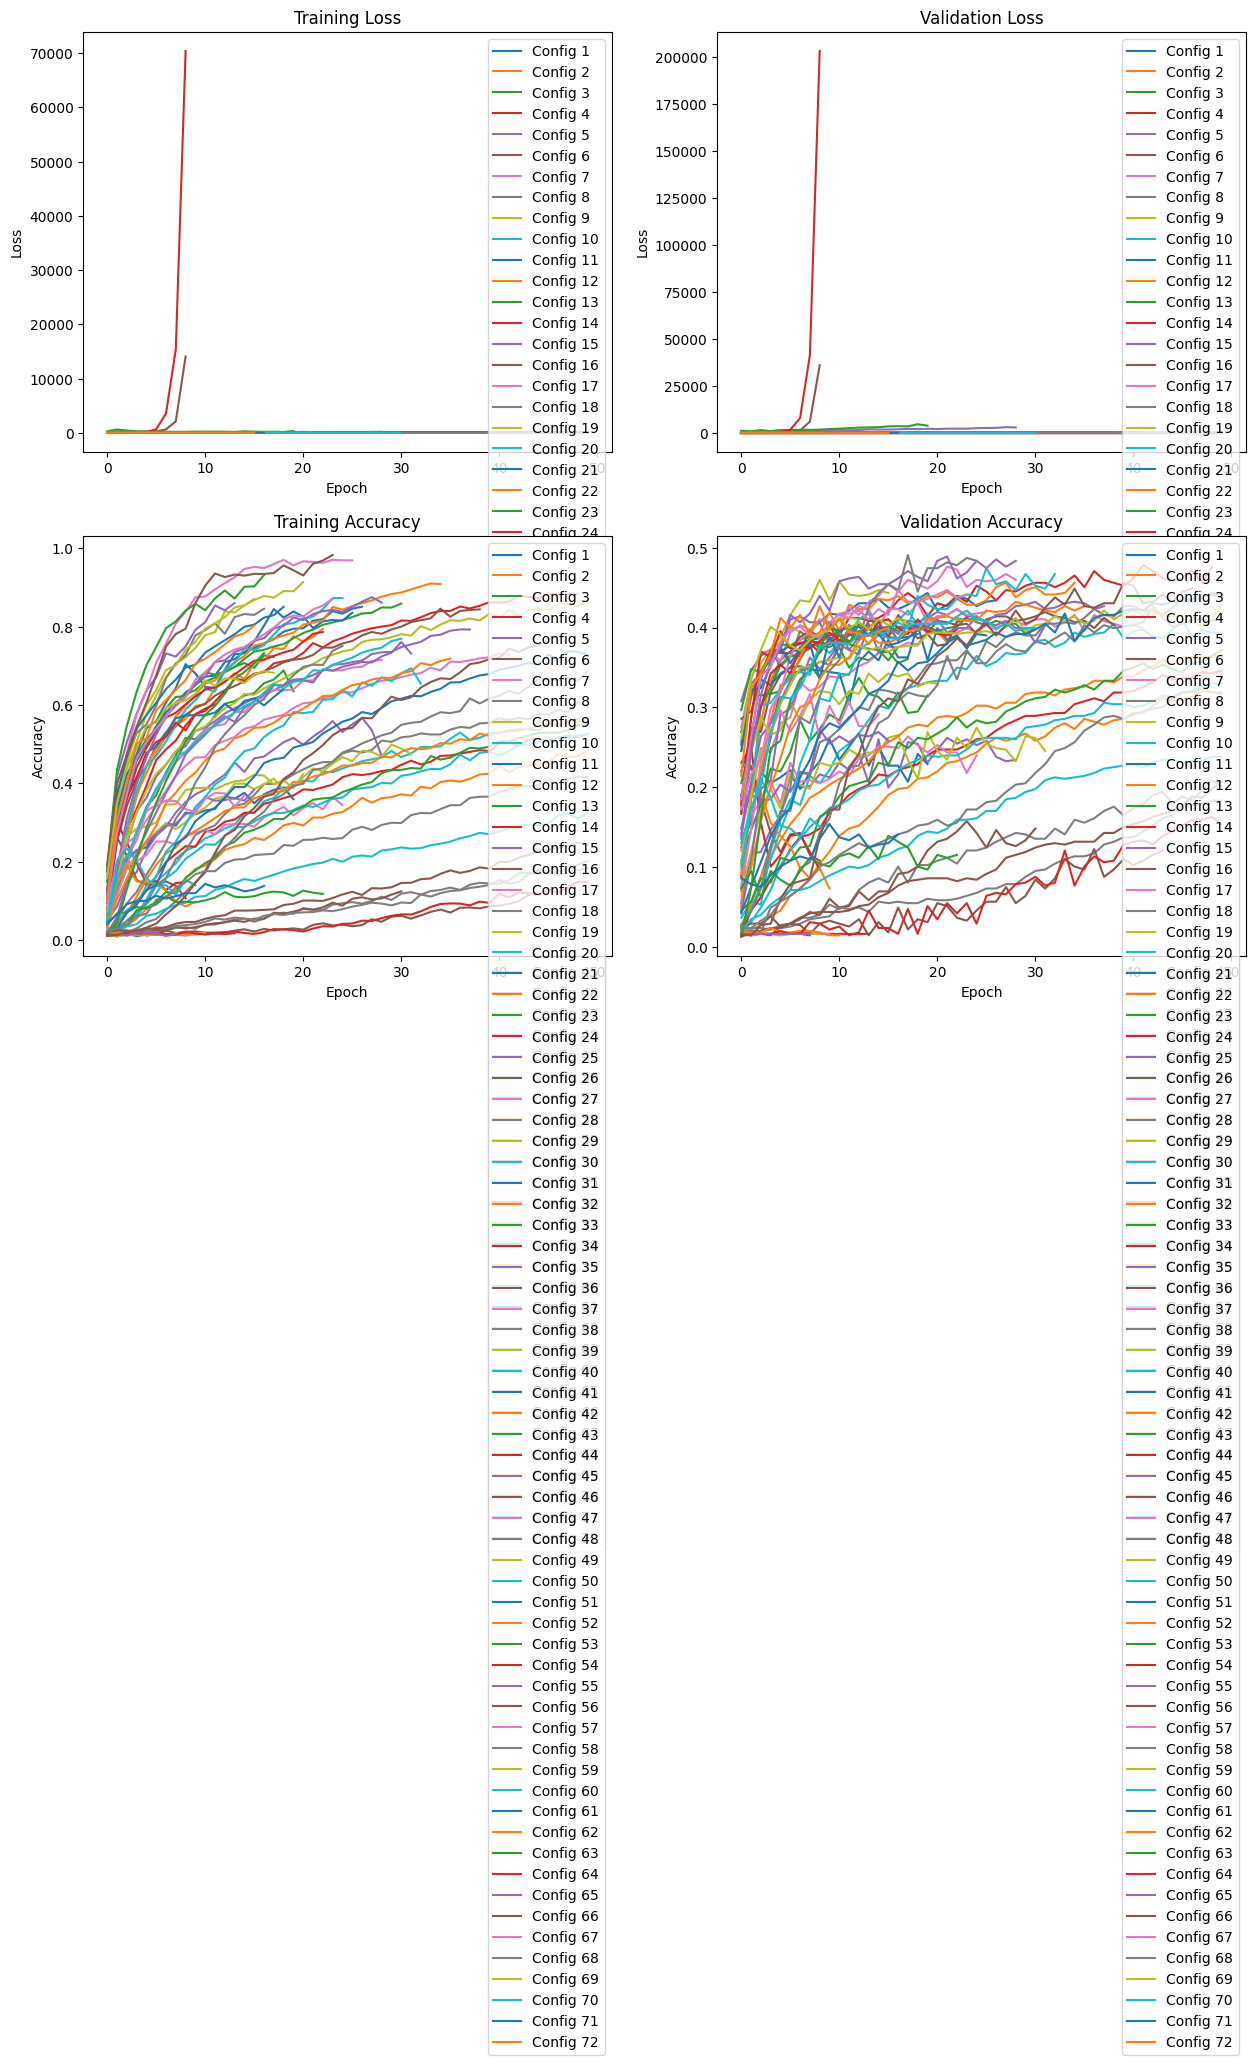
\includegraphics[width=469.5pt,height=772.5239pt]{latexImage_6893a42fd5858759c458902e916ccd85.png}}
\end{picture}
\newpage
\begin{tikzpicture}[overlay]
\path(0pt,0pt);
\filldraw[color_283006][even odd rule]
(21pt, -746pt) -- (561pt, -746pt)
 -- (561pt, -746pt)
 -- (561pt, -26pt)
 -- (561pt, -26pt)
 -- (21pt, -26pt) -- cycle
;
\begin{scope}
\clip
(32.25pt, -143.0006pt) -- (549.75pt, -143.0006pt)
 -- (549.75pt, -143.0006pt)
 -- (549.75pt, -41pt)
 -- (549.75pt, -41pt)
 -- (32.25pt, -41pt) -- cycle
;
\end{scope}
\end{tikzpicture}
\begin{picture}(-5,0)(2.5,0)
\put(84,-50.75043){\fontsize{9.75}{1}\usefont{T1}{cmr}{m}{n}\selectfont\color{color_29791}Training best model with optimal parameters...}
\put(84,-63.50049){\fontsize{9.75}{1}\usefont{T1}{cmr}{m}{n}\selectfont\color{color_29791}Epoch 10/100, Train Loss: 1.2180, Val Loss: 2.4536}
\put(84,-76.25061){\fontsize{9.75}{1}\usefont{T1}{cmr}{m}{n}\selectfont\color{color_29791}Train Acc: 0.6563, Val Acc: 0.4304}
\put(84,-89.00061){\fontsize{9.75}{1}\usefont{T1}{cmr}{m}{n}\selectfont\color{color_29791}Epoch 20/100, Train Loss: 0.6776, Val Loss: 2.8020}
\put(84,-101.7507){\fontsize{9.75}{1}\usefont{T1}{cmr}{m}{n}\selectfont\color{color_29791}Train Acc: 0.7933, Val Acc: 0.4835}
\put(84,-114.5008){\fontsize{9.75}{1}\usefont{T1}{cmr}{m}{n}\selectfont\color{color_29791}Epoch 30/100, Train Loss: 0.3969, Val Loss: 3.5192}
\put(84,-127.2509){\fontsize{9.75}{1}\usefont{T1}{cmr}{m}{n}\selectfont\color{color_29791}Train Acc: 0.8808, Val Acc: 0.5073}
\put(84,-140.0009){\fontsize{9.75}{1}\usefont{T1}{cmr}{m}{n}\selectfont\color{color_29791}Early stopping at epoch 40}
\put(80.25,-297.5036){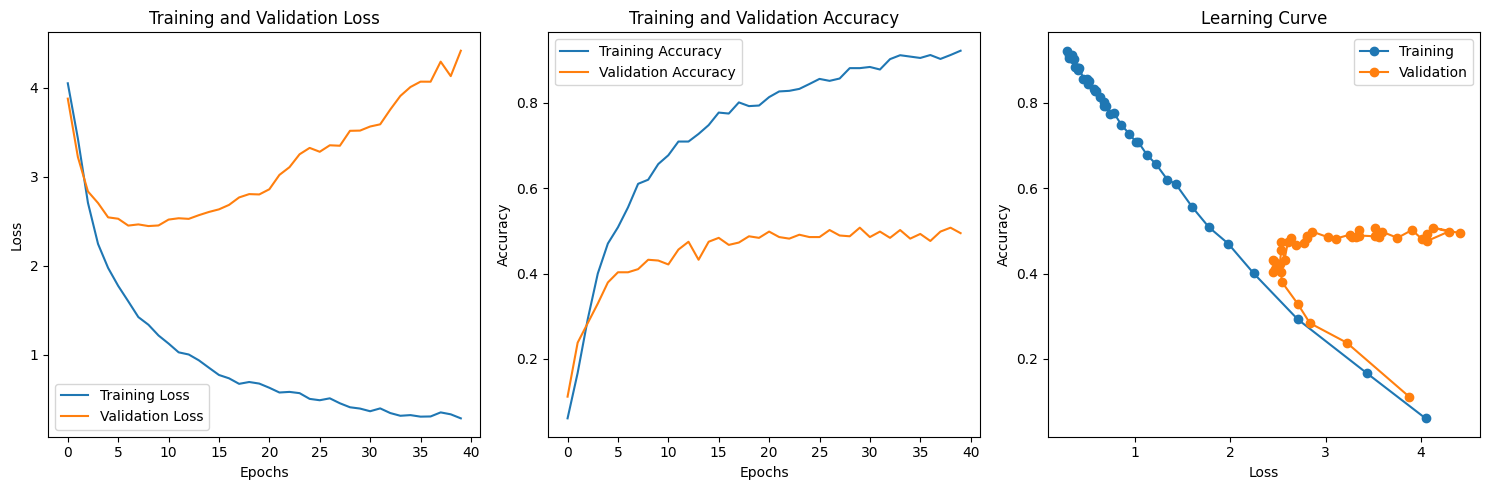
\includegraphics[width=469.5pt,height=154.503pt]{latexImage_19e9259ddfe0aa21ed1052c0100f9d8a.png}}
\put(84,-309.5535){\fontsize{9.75}{1}\usefont{T1}{cmr}{m}{n}\selectfont\color{color_29791}MLP Test Accuracy: 0.4971}
\put(84,-322.3035){\fontsize{9.75}{1}\usefont{T1}{cmr}{m}{n}\selectfont\color{color_29791}MLP Test Precision: 0.5204}
\put(84,-335.0536){\fontsize{9.75}{1}\usefont{T1}{cmr}{m}{n}\selectfont\color{color_29791}MLP Test Recall: 0.4971}
\put(84,-347.8037){\fontsize{9.75}{1}\usefont{T1}{cmr}{m}{n}\selectfont\color{color_29791}MLP Test F1-Score: 0.4962}
\end{picture}
\newpage
\begin{tikzpicture}[overlay]
\path(0pt,0pt);
\filldraw[color_283006][even odd rule]
(21pt, -746pt) -- (561pt, -746pt)
 -- (561pt, -746pt)
 -- (561pt, -26pt)
 -- (561pt, -26pt)
 -- (21pt, -26pt) -- cycle
;
\begin{scope}
\clip
(32.25pt, -465.2475pt) -- (549.75pt, -465.2475pt)
 -- (549.75pt, -465.2475pt)
 -- (549.75pt, -41pt)
 -- (549.75pt, -41pt)
 -- (32.25pt, -41pt) -- cycle
;
\end{scope}
\end{tikzpicture}
\begin{picture}(-5,0)(2.5,0)
\put(80.25,-462.9481){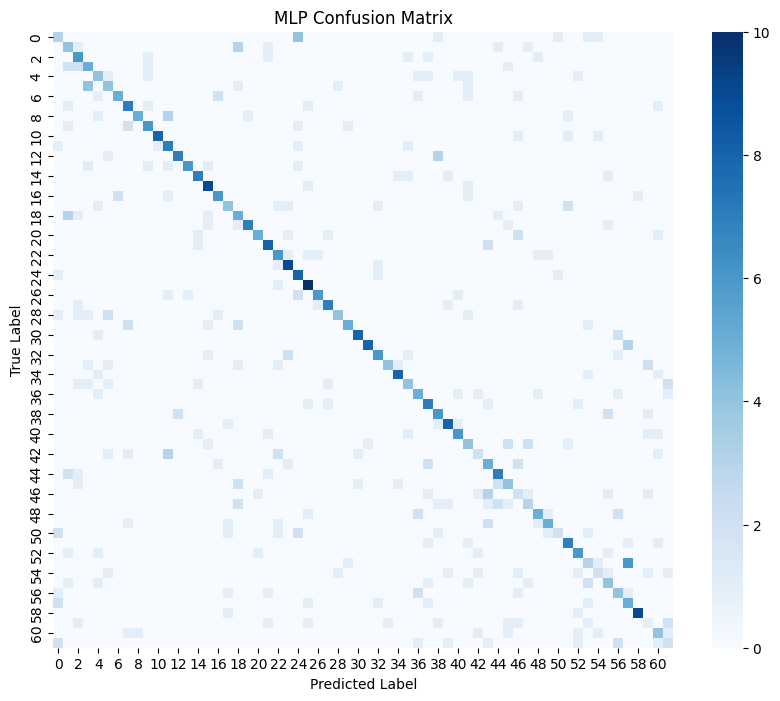
\includegraphics[width=469.5pt,height=421.9481pt]{latexImage_94569972310aa7fd518d7eb8e537199e.png}}
\put(80.25,-658.7336){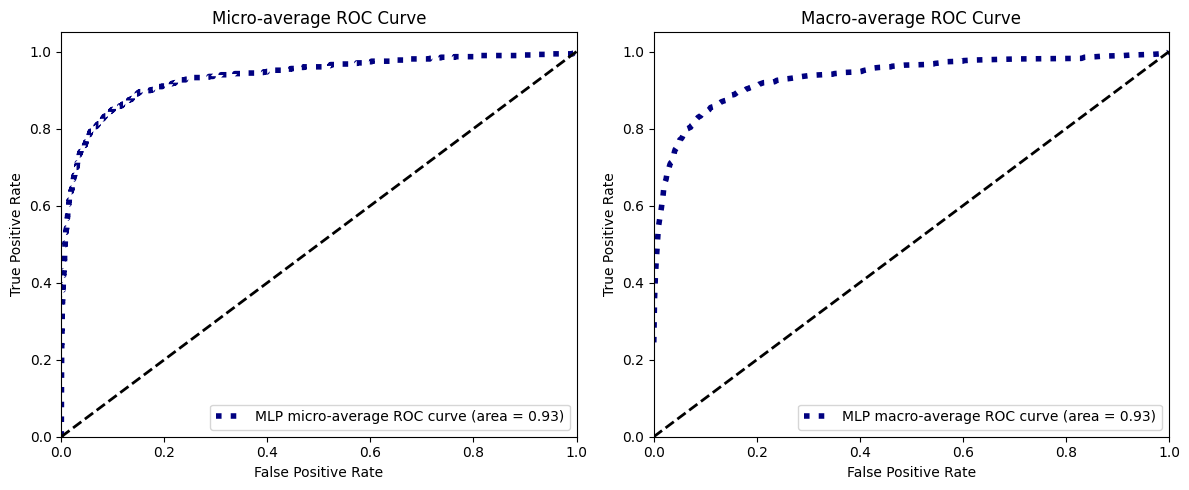
\includegraphics[width=469.5pt,height=193.4861pt]{latexImage_27c2c4df637f13a69a97397a9fbfa5cb.png}}
\end{picture}
\newpage
\begin{tikzpicture}[overlay]
\path(0pt,0pt);
\filldraw[color_283006][even odd rule]
(21pt, -746pt) -- (561pt, -746pt)
 -- (561pt, -746pt)
 -- (561pt, -26pt)
 -- (561pt, -26pt)
 -- (21pt, -26pt) -- cycle
;
\begin{scope}
\clip
(32.25pt, -729.5041pt) -- (549.75pt, -729.5041pt)
 -- (549.75pt, -729.5041pt)
 -- (549.75pt, -41pt)
 -- (549.75pt, -41pt)
 -- (32.25pt, -41pt) -- cycle
;
\end{scope}
\end{tikzpicture}
\begin{picture}(-5,0)(2.5,0)
\put(84,-50.75043){\fontsize{9.75}{1}\usefont{T1}{cmr}{m}{n}\selectfont\color{color_29791}Classification Report for MLP:}
\put(166.1799,-63.50049){\fontsize{9.75}{1}\usefont{T1}{cmr}{m}{n}\selectfont\color{color_29791}precision    recall  f1-score   support}
\put(148.5699,-89.00061){\fontsize{9.75}{1}\usefont{T1}{cmr}{m}{n}\selectfont\color{color_29791}0       0.23      0.27      0.25        11}
\put(148.5699,-101.7507){\fontsize{9.75}{1}\usefont{T1}{cmr}{m}{n}\selectfont\color{color_29791}1       0.27      0.36      0.31        11}
\put(148.5699,-114.5008){\fontsize{9.75}{1}\usefont{T1}{cmr}{m}{n}\selectfont\color{color_29791}2       0.38      0.55      0.44        11}
\put(148.5699,-127.2509){\fontsize{9.75}{1}\usefont{T1}{cmr}{m}{n}\selectfont\color{color_29791}3       0.38      0.45      0.42        11}
\put(148.5699,-140.0009){\fontsize{9.75}{1}\usefont{T1}{cmr}{m}{n}\selectfont\color{color_29791}4       0.33      0.36      0.35        11}
\put(148.5699,-152.751){\fontsize{9.75}{1}\usefont{T1}{cmr}{m}{n}\selectfont\color{color_29791}5       0.33      0.36      0.35        11}
\put(148.5699,-165.5011){\fontsize{9.75}{1}\usefont{T1}{cmr}{m}{n}\selectfont\color{color_29791}6       0.71      0.45      0.56        11}
\put(148.5699,-178.2512){\fontsize{9.75}{1}\usefont{T1}{cmr}{m}{n}\selectfont\color{color_29791}7       0.50      0.64      0.56        11}
\put(148.5699,-191.0012){\fontsize{9.75}{1}\usefont{T1}{cmr}{m}{n}\selectfont\color{color_29791}8       0.83      0.45      0.59        11}
\put(148.5699,-203.7513){\fontsize{9.75}{1}\usefont{T1}{cmr}{m}{n}\selectfont\color{color_29791}9       0.55      0.55      0.55        11}
\put(148.5699,-216.5014){\fontsize{9.75}{1}\usefont{T1}{cmr}{m}{n}\selectfont\color{color_29791}A       0.89      0.73      0.80        11}
\put(148.5699,-229.2515){\fontsize{9.75}{1}\usefont{T1}{cmr}{m}{n}\selectfont\color{color_29791}B       0.44      0.64      0.52        11}
\put(148.5699,-242.0015){\fontsize{9.75}{1}\usefont{T1}{cmr}{m}{n}\selectfont\color{color_29791}C       0.78      0.64      0.70        11}
\put(148.5699,-254.7516){\fontsize{9.75}{1}\usefont{T1}{cmr}{m}{n}\selectfont\color{color_29791}D       0.86      0.55      0.67        11}
\put(148.5699,-267.5017){\fontsize{9.75}{1}\usefont{T1}{cmr}{m}{n}\selectfont\color{color_29791}E       0.64      0.64      0.64        11}
\put(148.5699,-280.2518){\fontsize{9.75}{1}\usefont{T1}{cmr}{m}{n}\selectfont\color{color_29791}F       0.60      0.82      0.69        11}
\put(148.5699,-293.0018){\fontsize{9.75}{1}\usefont{T1}{cmr}{m}{n}\selectfont\color{color_29791}G       0.60      0.55      0.57        11}
\put(148.5699,-305.7519){\fontsize{9.75}{1}\usefont{T1}{cmr}{m}{n}\selectfont\color{color_29791}H       0.44      0.36      0.40        11}
\put(148.5699,-318.502){\fontsize{9.75}{1}\usefont{T1}{cmr}{m}{n}\selectfont\color{color_29791}I       0.29      0.45      0.36        11}
\put(148.5699,-331.2521){\fontsize{9.75}{1}\usefont{T1}{cmr}{m}{n}\selectfont\color{color_29791}J       0.88      0.64      0.74        11}
\put(148.5699,-344.0021){\fontsize{9.75}{1}\usefont{T1}{cmr}{m}{n}\selectfont\color{color_29791}K       0.71      0.45      0.56        11}
\put(148.5699,-356.7522){\fontsize{9.75}{1}\usefont{T1}{cmr}{m}{n}\selectfont\color{color_29791}L       0.57      0.73      0.64        11}
\put(148.5699,-369.5023){\fontsize{9.75}{1}\usefont{T1}{cmr}{m}{n}\selectfont\color{color_29791}M       0.43      0.55      0.48        11}
\put(148.5699,-382.2524){\fontsize{9.75}{1}\usefont{T1}{cmr}{m}{n}\selectfont\color{color_29791}N       0.60      0.82      0.69        11}
\put(148.5699,-395.0024){\fontsize{9.75}{1}\usefont{T1}{cmr}{m}{n}\selectfont\color{color_29791}O       0.42      0.73      0.53        11}
\put(148.5699,-407.7525){\fontsize{9.75}{1}\usefont{T1}{cmr}{m}{n}\selectfont\color{color_29791}P       0.59      0.91      0.71        11}
\put(148.5699,-420.5026){\fontsize{9.75}{1}\usefont{T1}{cmr}{m}{n}\selectfont\color{color_29791}Q       0.75      0.55      0.63        11}
\put(148.5699,-433.2527){\fontsize{9.75}{1}\usefont{T1}{cmr}{m}{n}\selectfont\color{color_29791}R       0.70      0.64      0.67        11}
\put(148.5699,-446.0027){\fontsize{9.75}{1}\usefont{T1}{cmr}{m}{n}\selectfont\color{color_29791}S       0.67      0.36      0.47        11}
\put(148.5699,-458.7528){\fontsize{9.75}{1}\usefont{T1}{cmr}{m}{n}\selectfont\color{color_29791}T       0.71      0.45      0.56        11}
\put(148.5699,-471.5029){\fontsize{9.75}{1}\usefont{T1}{cmr}{m}{n}\selectfont\color{color_29791}U       0.80      0.73      0.76        11}
\put(148.5699,-484.253){\fontsize{9.75}{1}\usefont{T1}{cmr}{m}{n}\selectfont\color{color_29791}V       0.89      0.73      0.80        11}
\put(148.5699,-497.003){\fontsize{9.75}{1}\usefont{T1}{cmr}{m}{n}\selectfont\color{color_29791}W       0.60      0.55      0.57        11}
\put(148.5699,-509.7531){\fontsize{9.75}{1}\usefont{T1}{cmr}{m}{n}\selectfont\color{color_29791}X       0.80      0.36      0.50        11}
\put(148.5699,-522.5032){\fontsize{9.75}{1}\usefont{T1}{cmr}{m}{n}\selectfont\color{color_29791}Y       0.73      0.73      0.73        11}
\put(148.5699,-535.2533){\fontsize{9.75}{1}\usefont{T1}{cmr}{m}{n}\selectfont\color{color_29791}Z       0.44      0.36      0.40        11}
\put(148.5699,-548.0033){\fontsize{9.75}{1}\usefont{T1}{cmr}{m}{n}\selectfont\color{color_29791}a       0.42      0.45      0.43        11}
\put(148.5699,-560.7534){\fontsize{9.75}{1}\usefont{T1}{cmr}{m}{n}\selectfont\color{color_29791}b       0.47      0.64      0.54        11}
\put(148.5699,-573.5035){\fontsize{9.75}{1}\usefont{T1}{cmr}{m}{n}\selectfont\color{color_29791}c       0.43      0.55      0.48        11}
\put(148.5699,-586.2536){\fontsize{9.75}{1}\usefont{T1}{cmr}{m}{n}\selectfont\color{color_29791}d       0.62      0.73      0.67        11}
\put(148.5699,-599.0036){\fontsize{9.75}{1}\usefont{T1}{cmr}{m}{n}\selectfont\color{color_29791}e       0.60      0.55      0.57        11}
\put(148.5699,-611.7537){\fontsize{9.75}{1}\usefont{T1}{cmr}{m}{n}\selectfont\color{color_29791}f       0.33      0.36      0.35        11}
\put(148.5699,-624.5038){\fontsize{9.75}{1}\usefont{T1}{cmr}{m}{n}\selectfont\color{color_29791}g       0.29      0.18      0.22        11}
\put(148.5699,-637.2539){\fontsize{9.75}{1}\usefont{T1}{cmr}{m}{n}\selectfont\color{color_29791}h       0.33      0.45      0.38        11}
\put(148.5699,-650.0039){\fontsize{9.75}{1}\usefont{T1}{cmr}{m}{n}\selectfont\color{color_29791}i       0.54      0.64      0.58        11}
\put(148.5699,-662.754){\fontsize{9.75}{1}\usefont{T1}{cmr}{m}{n}\selectfont\color{color_29791}j       0.36      0.36      0.36        11}
\put(148.5699,-675.5041){\fontsize{9.75}{1}\usefont{T1}{cmr}{m}{n}\selectfont\color{color_29791}k       0.15      0.18      0.17        11}
\put(148.5699,-688.2542){\fontsize{9.75}{1}\usefont{T1}{cmr}{m}{n}\selectfont\color{color_29791}l       0.38      0.27      0.32        11}
\put(148.5699,-701.0042){\fontsize{9.75}{1}\usefont{T1}{cmr}{m}{n}\selectfont\color{color_29791}m       0.56      0.45      0.50        11}
\put(148.5699,-713.7543){\fontsize{9.75}{1}\usefont{T1}{cmr}{m}{n}\selectfont\color{color_29791}n       0.62      0.45      0.53        11}
\put(148.5699,-726.5044){\fontsize{9.75}{1}\usefont{T1}{cmr}{m}{n}\selectfont\color{color_29791}o       0.50      0.18      0.27        11}
\end{picture}
\newpage
\begin{tikzpicture}[overlay]
\path(0pt,0pt);
\filldraw[color_283006][even odd rule]
(21pt, -746pt) -- (561pt, -746pt)
 -- (561pt, -746pt)
 -- (561pt, -26pt)
 -- (561pt, -26pt)
 -- (21pt, -26pt) -- cycle
;
\filldraw[color_273076][even odd rule]
(89.25pt, -724.0634pt) -- (549.75pt, -724.0634pt)
 -- (549.75pt, -724.0634pt)
 -- (549.75pt, -498.3121pt)
 -- (549.75pt, -498.3121pt)
 -- (89.25pt, -498.3121pt) -- cycle
;
\filldraw[color_252223][nonzero rule]
(89.25pt, -724.0634pt) -- (89.25pt, -498.3121pt)
 -- (89.25pt, -498.3121pt)
 -- (549.75pt, -498.3121pt)
 -- (549.75pt, -498.3121pt)
 -- (549.75pt, -724.0634pt)
 -- (549.75pt, -724.0634pt)
 -- (549pt, -724.0634pt)
 -- (549pt, -724.0634pt)
 -- (549pt, -499.0621pt)
 -- (549pt, -499.0621pt)
 -- (90pt, -499.0621pt)
 -- (90pt, -499.0621pt)
 -- (90pt, -724.0634pt) -- cycle
;
\begin{scope}
\clip
(32.25pt, -724.0634pt) -- (549.75pt, -724.0634pt)
 -- (549.75pt, -724.0634pt)
 -- (549.75pt, -498.3121pt)
 -- (549.75pt, -498.3121pt)
 -- (32.25pt, -498.3121pt) -- cycle
;
\begin{scope}
\clip
(90pt, -723.3134pt) -- (549pt, -723.3134pt)
 -- (549pt, -723.3134pt)
 -- (549pt, -499.0621pt)
 -- (549pt, -499.0621pt)
 -- (90pt, -499.0621pt) -- cycle
;
\filldraw[color_273076][even odd rule]
(90pt, -723.3134pt) -- (549pt, -723.3134pt)
 -- (549pt, -723.3134pt)
 -- (549pt, -499.0621pt)
 -- (549pt, -499.0621pt)
 -- (90pt, -499.0621pt) -- cycle
;
\end{scope}
\end{scope}
\begin{scope}
\clip
(32.25pt, -245.0012pt) -- (549.75pt, -245.0012pt)
 -- (549.75pt, -245.0012pt)
 -- (549.75pt, -41pt)
 -- (549.75pt, -41pt)
 -- (32.25pt, -41pt) -- cycle
;
\end{scope}
\end{tikzpicture}
\begin{picture}(-5,0)(2.5,0)
\put(148.5699,-50.75043){\fontsize{9.75}{1}\usefont{T1}{cmr}{m}{n}\selectfont\color{color_29791}p       0.58      0.64      0.61        11}
\put(148.5699,-63.50049){\fontsize{9.75}{1}\usefont{T1}{cmr}{m}{n}\selectfont\color{color_29791}q       0.50      0.55      0.52        11}
\put(148.5699,-76.25061){\fontsize{9.75}{1}\usefont{T1}{cmr}{m}{n}\selectfont\color{color_29791}r       0.27      0.27      0.27        11}
\put(148.5699,-89.00061){\fontsize{9.75}{1}\usefont{T1}{cmr}{m}{n}\selectfont\color{color_29791}s       0.33      0.18      0.24        11}
\put(148.5699,-101.7507){\fontsize{9.75}{1}\usefont{T1}{cmr}{m}{n}\selectfont\color{color_29791}t       0.36      0.36      0.36        11}
\put(148.5699,-114.5008){\fontsize{9.75}{1}\usefont{T1}{cmr}{m}{n}\selectfont\color{color_29791}u       0.33      0.36      0.35        11}
\put(148.5699,-127.2509){\fontsize{9.75}{1}\usefont{T1}{cmr}{m}{n}\selectfont\color{color_29791}v       0.31      0.45      0.37        11}
\put(148.5699,-140.0009){\fontsize{9.75}{1}\usefont{T1}{cmr}{m}{n}\selectfont\color{color_29791}w       0.90      0.82      0.86        11}
\put(148.5699,-152.751){\fontsize{9.75}{1}\usefont{T1}{cmr}{m}{n}\selectfont\color{color_29791}x       0.14      0.09      0.11        11}
\put(148.5699,-165.5011){\fontsize{9.75}{1}\usefont{T1}{cmr}{m}{n}\selectfont\color{color_29791}y       0.36      0.36      0.36        11}
\put(148.5699,-178.2512){\fontsize{9.75}{1}\usefont{T1}{cmr}{m}{n}\selectfont\color{color_29791}z       0.22      0.18      0.20        11}
\put(107.48,-203.7513){\fontsize{9.75}{1}\usefont{T1}{cmr}{m}{n}\selectfont\color{color_29791}accuracy                           0.50       682}
\put(101.61,-216.5014){\fontsize{9.75}{1}\usefont{T1}{cmr}{m}{n}\selectfont\color{color_29791}macro avg       0.52      0.50      0.50       682}
\put(84,-229.2515){\fontsize{9.75}{1}\usefont{T1}{cmr}{m}{n}\selectfont\color{color_29791}weighted avg       0.52      0.50      0.50       682}
\put(80.25,-437.467){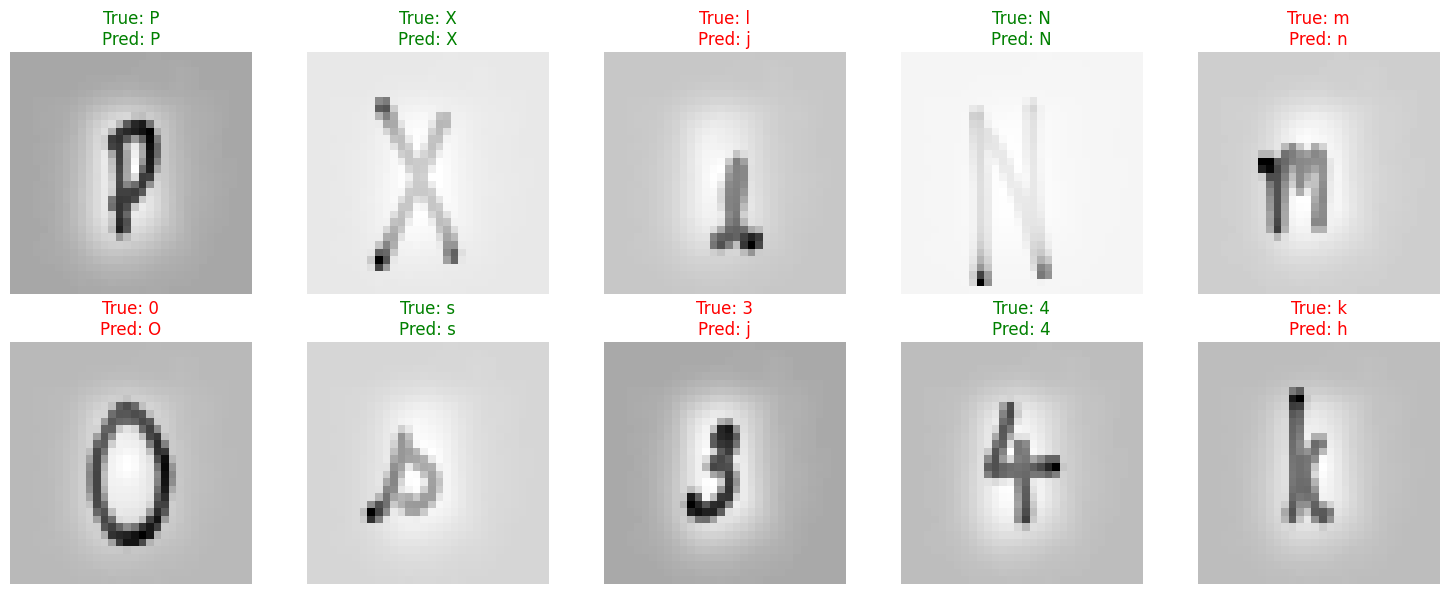
\includegraphics[width=469.5pt,height=192.4658pt]{latexImage_f41dc7f31965011d71eaab130f257b71.png}}
\put(93,-478.7541){\fontsize{21.7728}{1}\usefont{T1}{cmr}{b}{n}\selectfont\color{color_29791}4. Hyperparameter Tuning}
\put(93,-512.5625){\fontsize{9.75}{1}\usefont{T1}{cmr}{m}{n}\selectfont\color{color_95391}\# Define hyperparameters to tune}
\put(93,-525.3126){\fontsize{9.75}{1}\usefont{T1}{cmr}{m}{n}\selectfont\color{color_62560}hidden\_layers\_options=[[128],[256],[128,64],[256,128]]}
\put(93,-538.0626){\fontsize{9.75}{1}\usefont{T1}{cmr}{m}{n}\selectfont\color{color_62560}activation\_options=['relu','sigmoid','tanh']}
\put(93,-550.8127){\fontsize{9.75}{1}\usefont{T1}{cmr}{m}{n}\selectfont\color{color_62560}learning\_rates=[0.001,0.01,0.1]}
\put(93,-563.5628){\fontsize{9.75}{1}\usefont{T1}{cmr}{m}{n}\selectfont\color{color_62560}optimizers\_list=['adam','sgd']}
\put(93,-589.0629){\fontsize{9.75}{1}\usefont{T1}{cmr}{m}{n}\selectfont\color{color_95391}\# Tuning loop}
\put(93,-601.813){\fontsize{9.75}{1}\usefont{T1}{cmr}{m}{n}\selectfont\color{color_62560}best\_val\_acc=0}
\put(93,-614.5631){\fontsize{9.75}{1}\usefont{T1}{cmr}{m}{n}\selectfont\color{color_62560}best\_params=\{\}}
\put(93,-627.3132){\fontsize{9.75}{1}\usefont{T1}{cmr}{m}{n}\selectfont\color{color_62560}best\_model=None}
\put(93,-640.0632){\fontsize{9.75}{1}\usefont{T1}{cmr}{m}{n}\selectfont\color{color_62560}all\_results=[]}
\put(93,-665.5634){\fontsize{9.75}{1}\usefont{T1}{cmr}{m}{n}\selectfont\color{color_62560}print("Starting hyperparameter tuning...")}
\put(93,-691.0635){\fontsize{9.75}{1}\usefont{T1}{cmr}{b}{n}\selectfont\color{color_33759}forhidden\_layersinhidden\_layers\_options:}
\put(116.48,-703.8136){\fontsize{9.75}{1}\usefont{T1}{cmr}{b}{n}\selectfont\color{color_33759}foractivationinactivation\_options:}
\put(139.96,-716.5637){\fontsize{9.75}{1}\usefont{T1}{cmr}{b}{n}\selectfont\color{color_33759}forlrinlearning\_rates:}
\put(43.66,-512.5625){\fontsize{9.75}{1}\usefont{T1}{cmr}{m}{n}\selectfont\color{color_126112}In[8]:}
\end{picture}
\newpage
\begin{tikzpicture}[overlay]
\path(0pt,0pt);
\filldraw[color_283006][even odd rule]
(21pt, -746pt) -- (561pt, -746pt)
 -- (561pt, -746pt)
 -- (561pt, -26pt)
 -- (561pt, -26pt)
 -- (21pt, -26pt) -- cycle
;
\filldraw[color_273076][even odd rule]
(89.25pt, -722.004pt) -- (549.75pt, -722.004pt)
 -- (549.75pt, -722.004pt)
 -- (549.75pt, -37.25pt)
 -- (549.75pt, -37.25pt)
 -- (89.25pt, -37.25pt) -- cycle
;
\filldraw[color_252223][nonzero rule]
(89.25pt, -722.004pt) -- (90pt, -722.004pt)
 -- (90pt, -722.004pt)
 -- (90pt, -37.25pt)
 -- (90pt, -37.25pt)
 -- (89.25pt, -37.25pt) -- cycle
;
\filldraw[color_252223][nonzero rule]
(549pt, -722.004pt) -- (549.75pt, -722.004pt)
 -- (549.75pt, -722.004pt)
 -- (549.75pt, -37.25pt)
 -- (549.75pt, -37.25pt)
 -- (549pt, -37.25pt) -- cycle
;
\begin{scope}
\clip
(32.25pt, -722.004pt) -- (549.75pt, -722.004pt)
 -- (549.75pt, -722.004pt)
 -- (549.75pt, -37.25pt)
 -- (549.75pt, -37.25pt)
 -- (32.25pt, -37.25pt) -- cycle
;
\begin{scope}
\clip
(90pt, -721.254pt) -- (549pt, -721.254pt)
 -- (549pt, -721.254pt)
 -- (549pt, -38pt)
 -- (549pt, -38pt)
 -- (90pt, -38pt) -- cycle
;
\filldraw[color_273076][even odd rule]
(90pt, -721.254pt) -- (549pt, -721.254pt)
 -- (549pt, -721.254pt)
 -- (549pt, -38pt)
 -- (549pt, -38pt)
 -- (90pt, -38pt) -- cycle
;
\end{scope}
\end{scope}
\begin{scope}
\clip
(32.25pt, -722.004pt) -- (549.75pt, -722.004pt)
 -- (549.75pt, -722.004pt)
 -- (549.75pt, -37.25pt)
 -- (549.75pt, -37.25pt)
 -- (32.25pt, -37.25pt) -- cycle
;
\begin{scope}
\clip
(90pt, -721.254pt) -- (549pt, -721.254pt)
 -- (549pt, -721.254pt)
 -- (549pt, -38pt)
 -- (549pt, -38pt)
 -- (90pt, -38pt) -- cycle
;
\end{scope}
\end{scope}
\end{tikzpicture}
\begin{picture}(-5,0)(2.5,0)
\put(163.4399,-51.50043){\fontsize{9.75}{1}\usefont{T1}{cmr}{b}{n}\selectfont\color{color_33759}foropt\_nameinoptimizers\_list:}
\put(186.9199,-64.25049){\fontsize{9.75}{1}\usefont{T1}{cmr}{m}{n}\selectfont\color{color_62560}print(f"Testing: Layers=\{hidden\_layers\}, Activation=\{activation}
\put(186.9199,-89.75061){\fontsize{9.75}{1}\usefont{T1}{cmr}{m}{n}\selectfont\color{color_95391}\# Initialize model}
\put(186.9199,-102.5007){\fontsize{9.75}{1}\usefont{T1}{cmr}{m}{n}\selectfont\color{color_62560}model=MLP(input\_size,hidden\_layers,num\_classes,activation=}
\put(186.9199,-128.0009){\fontsize{9.75}{1}\usefont{T1}{cmr}{m}{n}\selectfont\color{color_95391}\# Define loss and optimizer}
\put(186.9199,-140.7509){\fontsize{9.75}{1}\usefont{T1}{cmr}{m}{n}\selectfont\color{color_62560}criterion=nn.CrossEntropyLoss()}
\put(186.9199,-166.2511){\fontsize{9.75}{1}\usefont{T1}{cmr}{b}{n}\selectfont\color{color_33759}ifopt\_name=='adam':}
\put(210.3999,-179.0012){\fontsize{9.75}{1}\usefont{T1}{cmr}{m}{n}\selectfont\color{color_62560}optimizer=optim.Adam(model.parameters(),lr=lr)}
\put(186.9199,-191.7512){\fontsize{9.75}{1}\usefont{T1}{cmr}{b}{n}\selectfont\color{color_33759}else:}
\put(210.3999,-204.5013){\fontsize{9.75}{1}\usefont{T1}{cmr}{m}{n}\selectfont\color{color_62560}optimizer=optim.SGD(model.parameters(),lr=lr,momentum=0.9}
\put(186.9199,-230.0015){\fontsize{9.75}{1}\usefont{T1}{cmr}{m}{n}\selectfont\color{color_95391}\# Train model}
\put(186.9199,-242.7515){\fontsize{9.75}{1}\usefont{T1}{cmr}{m}{n}\selectfont\color{color_62560}model,train\_losses,val\_losses,train\_accs,val\_accs=train\_model}
\put(210.3999,-255.5016){\fontsize{9.75}{1}\usefont{T1}{cmr}{m}{n}\selectfont\color{color_62560}model,train\_loader,val\_loader,criterion,optimizer,}
\put(210.3999,-268.2517){\fontsize{9.75}{1}\usefont{T1}{cmr}{m}{n}\selectfont\color{color_62560}num\_epochs=50,patience=7}
\put(186.9199,-281.0018){\fontsize{9.75}{1}\usefont{T1}{cmr}{m}{n}\selectfont\color{color_32596})}
\put(186.9199,-306.5019){\fontsize{9.75}{1}\usefont{T1}{cmr}{m}{n}\selectfont\color{color_95391}\# Evaluate on validation set}
\put(186.9199,-319.252){\fontsize{9.75}{1}\usefont{T1}{cmr}{m}{n}\selectfont\color{color_62560}val\_acc,\_,\_,\_=evaluate\_model(model,val\_loader)}
\put(186.9199,-344.7521){\fontsize{9.75}{1}\usefont{T1}{cmr}{m}{n}\selectfont\color{color_62560}print(f"Validation Accuracy:\{val\_acc:.4f\}")}
\put(186.9199,-370.2523){\fontsize{9.75}{1}\usefont{T1}{cmr}{m}{n}\selectfont\color{color_95391}\# Store results}
\put(186.9199,-383.0024){\fontsize{9.75}{1}\usefont{T1}{cmr}{m}{n}\selectfont\color{color_62560}result=\{}
\put(210.3999,-395.7524){\fontsize{9.75}{1}\usefont{T1}{cmr}{m}{n}\selectfont\color{color_209593}'hidden\_layers':hidden\_layers,}
\put(210.3999,-408.5025){\fontsize{9.75}{1}\usefont{T1}{cmr}{m}{n}\selectfont\color{color_209593}'activation':activation,}
\put(210.3999,-421.2526){\fontsize{9.75}{1}\usefont{T1}{cmr}{m}{n}\selectfont\color{color_209593}'learning\_rate':lr,}
\put(210.3999,-434.0027){\fontsize{9.75}{1}\usefont{T1}{cmr}{m}{n}\selectfont\color{color_209593}'optimizer':opt\_name,}
\put(210.3999,-446.7527){\fontsize{9.75}{1}\usefont{T1}{cmr}{m}{n}\selectfont\color{color_209593}'val\_accuracy':val\_acc,}
\put(210.3999,-459.5028){\fontsize{9.75}{1}\usefont{T1}{cmr}{m}{n}\selectfont\color{color_209593}'train\_losses':train\_losses,}
\put(210.3999,-472.2529){\fontsize{9.75}{1}\usefont{T1}{cmr}{m}{n}\selectfont\color{color_209593}'val\_losses':val\_losses,}
\put(210.3999,-485.003){\fontsize{9.75}{1}\usefont{T1}{cmr}{m}{n}\selectfont\color{color_209593}'train\_accs':train\_accs,}
\put(210.3999,-497.753){\fontsize{9.75}{1}\usefont{T1}{cmr}{m}{n}\selectfont\color{color_209593}'val\_accs':val\_accs}
\put(186.9199,-510.5031){\fontsize{9.75}{1}\usefont{T1}{cmr}{m}{n}\selectfont\color{color_32596}\}}
\put(186.9199,-523.2532){\fontsize{9.75}{1}\usefont{T1}{cmr}{m}{n}\selectfont\color{color_62560}all\_results.append(result)}
\put(186.9199,-548.7533){\fontsize{9.75}{1}\usefont{T1}{cmr}{m}{n}\selectfont\color{color_95391}\# Update best model}
\put(186.9199,-561.5034){\fontsize{9.75}{1}\usefont{T1}{cmr}{b}{n}\selectfont\color{color_33759}ifval\_acc>best\_val\_acc:}
\put(210.3999,-574.2535){\fontsize{9.75}{1}\usefont{T1}{cmr}{m}{n}\selectfont\color{color_62560}best\_val\_acc=val\_acc}
\put(210.3999,-587.0036){\fontsize{9.75}{1}\usefont{T1}{cmr}{m}{n}\selectfont\color{color_62560}best\_params=\{}
\put(233.8799,-599.7536){\fontsize{9.75}{1}\usefont{T1}{cmr}{m}{n}\selectfont\color{color_209593}'hidden\_layers':hidden\_layers,}
\put(233.8799,-612.5037){\fontsize{9.75}{1}\usefont{T1}{cmr}{m}{n}\selectfont\color{color_209593}'activation':activation,}
\put(233.8799,-625.2538){\fontsize{9.75}{1}\usefont{T1}{cmr}{m}{n}\selectfont\color{color_209593}'learning\_rate':lr,}
\put(233.8799,-638.0039){\fontsize{9.75}{1}\usefont{T1}{cmr}{m}{n}\selectfont\color{color_209593}'optimizer':opt\_name}
\put(210.3999,-650.7539){\fontsize{9.75}{1}\usefont{T1}{cmr}{m}{n}\selectfont\color{color_32596}\}}
\put(210.3999,-663.504){\fontsize{9.75}{1}\usefont{T1}{cmr}{m}{n}\selectfont\color{color_62560}best\_model=model}
\put(210.3999,-676.2541){\fontsize{9.75}{1}\usefont{T1}{cmr}{m}{n}\selectfont\color{color_62560}print("New best model found!")}
\put(93,-701.7542){\fontsize{9.75}{1}\usefont{T1}{cmr}{m}{n}\selectfont\color{color_62560}print("Tuning completed!")}
\put(93,-714.5043){\fontsize{9.75}{1}\usefont{T1}{cmr}{m}{n}\selectfont\color{color_62560}print(f"Best validation accuracy:\{best\_val\_acc:.4f\}")}
\end{picture}
\newpage
\begin{tikzpicture}[overlay]
\path(0pt,0pt);
\filldraw[color_283006][even odd rule]
(21pt, -746pt) -- (561pt, -746pt)
 -- (561pt, -746pt)
 -- (561pt, -26pt)
 -- (561pt, -26pt)
 -- (21pt, -26pt) -- cycle
;
\filldraw[color_273076][even odd rule]
(89.25pt, -479.7526pt) -- (549.75pt, -479.7526pt)
 -- (549.75pt, -479.7526pt)
 -- (549.75pt, -37.25pt)
 -- (549.75pt, -37.25pt)
 -- (89.25pt, -37.25pt) -- cycle
;
\filldraw[color_252223][nonzero rule]
(549.75pt, -37.25pt) -- (549.75pt, -479.7526pt)
 -- (549.75pt, -479.7526pt)
 -- (89.25pt, -479.7526pt)
 -- (89.25pt, -479.7526pt)
 -- (89.25pt, -37.25pt)
 -- (89.25pt, -37.25pt)
 -- (90pt, -37.25pt)
 -- (90pt, -37.25pt)
 -- (90pt, -479.0026pt)
 -- (90pt, -479.0026pt)
 -- (549pt, -479.0026pt)
 -- (549pt, -479.0026pt)
 -- (549pt, -37.25pt) -- cycle
;
\begin{scope}
\clip
(32.25pt, -479.7526pt) -- (549.75pt, -479.7526pt)
 -- (549.75pt, -479.7526pt)
 -- (549.75pt, -37.25pt)
 -- (549.75pt, -37.25pt)
 -- (32.25pt, -37.25pt) -- cycle
;
\begin{scope}
\clip
(90pt, -479.0026pt) -- (549pt, -479.0026pt)
 -- (549pt, -479.0026pt)
 -- (549pt, -38pt)
 -- (549pt, -38pt)
 -- (90pt, -38pt) -- cycle
;
\filldraw[color_273076][even odd rule]
(90pt, -479.0026pt) -- (549pt, -479.0026pt)
 -- (549pt, -479.0026pt)
 -- (549pt, -38pt)
 -- (549pt, -38pt)
 -- (90pt, -38pt) -- cycle
;
\end{scope}
\end{scope}
\begin{scope}
\clip
(32.25pt, -479.7526pt) -- (549.75pt, -479.7526pt)
 -- (549.75pt, -479.7526pt)
 -- (549.75pt, -37.25pt)
 -- (549.75pt, -37.25pt)
 -- (32.25pt, -37.25pt) -- cycle
;
\begin{scope}
\clip
(90pt, -479.0026pt) -- (549pt, -479.0026pt)
 -- (549pt, -479.0026pt)
 -- (549pt, -38pt)
 -- (549pt, -38pt)
 -- (90pt, -38pt) -- cycle
;
\end{scope}
\end{scope}
\end{tikzpicture}
\begin{picture}(-5,0)(2.5,0)
\put(93,-51.50043){\fontsize{9.75}{1}\usefont{T1}{cmr}{m}{n}\selectfont\color{color_62560}print(f"Best parameters:\{best\_params\}")}
\put(93,-77.00061){\fontsize{9.75}{1}\usefont{T1}{cmr}{m}{n}\selectfont\color{color_95391}\# Plot training curves for all configurations}
\put(93,-89.75061){\fontsize{9.75}{1}\usefont{T1}{cmr}{m}{n}\selectfont\color{color_62560}fig,axes=plt.subplots(2,2,figsize=(15,12))}
\put(93,-102.5007){\fontsize{9.75}{1}\usefont{T1}{cmr}{m}{n}\selectfont\color{color_62560}axes=axes.flatten()}
\put(93,-128.0009){\fontsize{9.75}{1}\usefont{T1}{cmr}{b}{n}\selectfont\color{color_33759}fori,resultinenumerate(all\_results):}
\put(116.48,-140.7509){\fontsize{9.75}{1}\usefont{T1}{cmr}{m}{n}\selectfont\color{color_62560}axes[0].plot(result['train\_losses'],label=f"Config\{i+1\}")}
\put(116.48,-153.501){\fontsize{9.75}{1}\usefont{T1}{cmr}{m}{n}\selectfont\color{color_62560}axes[1].plot(result['val\_losses'],label=f"Config\{i+1\}")}
\put(116.48,-166.2511){\fontsize{9.75}{1}\usefont{T1}{cmr}{m}{n}\selectfont\color{color_62560}axes[2].plot(result['train\_accs'],label=f"Config\{i+1\}")}
\put(116.48,-179.0012){\fontsize{9.75}{1}\usefont{T1}{cmr}{m}{n}\selectfont\color{color_62560}axes[3].plot(result['val\_accs'],label=f"Config\{i+1\}")}
\put(93,-204.5013){\fontsize{9.75}{1}\usefont{T1}{cmr}{m}{n}\selectfont\color{color_62560}axes[0].set\_title('Training Loss')}
\put(93,-217.2514){\fontsize{9.75}{1}\usefont{T1}{cmr}{m}{n}\selectfont\color{color_62560}axes[0].set\_xlabel('Epoch')}
\put(93,-230.0015){\fontsize{9.75}{1}\usefont{T1}{cmr}{m}{n}\selectfont\color{color_62560}axes[0].set\_ylabel('Loss')}
\put(93,-242.7515){\fontsize{9.75}{1}\usefont{T1}{cmr}{m}{n}\selectfont\color{color_62560}axes[0].legend()}
\put(93,-268.2517){\fontsize{9.75}{1}\usefont{T1}{cmr}{m}{n}\selectfont\color{color_62560}axes[1].set\_title('Validation Loss')}
\put(93,-281.0018){\fontsize{9.75}{1}\usefont{T1}{cmr}{m}{n}\selectfont\color{color_62560}axes[1].set\_xlabel('Epoch')}
\put(93,-293.7518){\fontsize{9.75}{1}\usefont{T1}{cmr}{m}{n}\selectfont\color{color_62560}axes[1].set\_ylabel('Loss')}
\put(93,-306.5019){\fontsize{9.75}{1}\usefont{T1}{cmr}{m}{n}\selectfont\color{color_62560}axes[1].legend()}
\put(93,-332.0021){\fontsize{9.75}{1}\usefont{T1}{cmr}{m}{n}\selectfont\color{color_62560}axes[2].set\_title('Training Accuracy')}
\put(93,-344.7521){\fontsize{9.75}{1}\usefont{T1}{cmr}{m}{n}\selectfont\color{color_62560}axes[2].set\_xlabel('Epoch')}
\put(93,-357.5022){\fontsize{9.75}{1}\usefont{T1}{cmr}{m}{n}\selectfont\color{color_62560}axes[2].set\_ylabel('Accuracy')}
\put(93,-370.2523){\fontsize{9.75}{1}\usefont{T1}{cmr}{m}{n}\selectfont\color{color_62560}axes[2].legend()}
\put(93,-395.7524){\fontsize{9.75}{1}\usefont{T1}{cmr}{m}{n}\selectfont\color{color_62560}axes[3].set\_title('Validation Accuracy')}
\put(93,-408.5025){\fontsize{9.75}{1}\usefont{T1}{cmr}{m}{n}\selectfont\color{color_62560}axes[3].set\_xlabel('Epoch')}
\put(93,-421.2526){\fontsize{9.75}{1}\usefont{T1}{cmr}{m}{n}\selectfont\color{color_62560}axes[3].set\_ylabel('Accuracy')}
\put(93,-434.0027){\fontsize{9.75}{1}\usefont{T1}{cmr}{m}{n}\selectfont\color{color_62560}axes[3].legend()}
\put(93,-459.5028){\fontsize{9.75}{1}\usefont{T1}{cmr}{m}{n}\selectfont\color{color_62560}plt.tight\_layout()}
\put(93,-472.2529){\fontsize{9.75}{1}\usefont{T1}{cmr}{m}{n}\selectfont\color{color_62560}plt.show()}
\end{picture}
\newpage
\begin{tikzpicture}[overlay]
\path(0pt,0pt);
\filldraw[color_283006][even odd rule]
(21pt, -746pt) -- (561pt, -746pt)
 -- (561pt, -746pt)
 -- (561pt, -26pt)
 -- (561pt, -26pt)
 -- (21pt, -26pt) -- cycle
;
\begin{scope}
\clip
(32.25pt, -729.5041pt) -- (549.75pt, -729.5041pt)
 -- (549.75pt, -729.5041pt)
 -- (549.75pt, -41pt)
 -- (549.75pt, -41pt)
 -- (32.25pt, -41pt) -- cycle
;
\end{scope}
\end{tikzpicture}
\begin{picture}(-5,0)(2.5,0)
\put(84,-50.75043){\fontsize{9.75}{1}\usefont{T1}{cmr}{m}{n}\selectfont\color{color_29791}Starting hyperparameter tuning...}
\put(84,-63.50049){\fontsize{9.75}{1}\usefont{T1}{cmr}{m}{n}\selectfont\color{color_29791}Testing: Layers=[128], Activation=relu, LR=0.001, Optimizer=adam}
\put(84,-76.25061){\fontsize{9.75}{1}\usefont{T1}{cmr}{m}{n}\selectfont\color{color_29791}Epoch 10/50, Train Loss: 1.3568, Val Loss: 2.5266}
\put(84,-89.00061){\fontsize{9.75}{1}\usefont{T1}{cmr}{m}{n}\selectfont\color{color_29791}Train Acc: 0.6554, Val Acc: 0.4066}
\put(84,-101.7507){\fontsize{9.75}{1}\usefont{T1}{cmr}{m}{n}\selectfont\color{color_29791}Epoch 20/50, Train Loss: 0.8028, Val Loss: 2.6862}
\put(84,-114.5008){\fontsize{9.75}{1}\usefont{T1}{cmr}{m}{n}\selectfont\color{color_29791}Train Acc: 0.7933, Val Acc: 0.4322}
\put(84,-127.2509){\fontsize{9.75}{1}\usefont{T1}{cmr}{m}{n}\selectfont\color{color_29791}Epoch 30/50, Train Loss: 0.5172, Val Loss: 2.9831}
\put(84,-140.0009){\fontsize{9.75}{1}\usefont{T1}{cmr}{m}{n}\selectfont\color{color_29791}Train Acc: 0.8731, Val Acc: 0.4304}
\put(84,-152.751){\fontsize{9.75}{1}\usefont{T1}{cmr}{m}{n}\selectfont\color{color_29791}Early stopping at epoch 31}
\put(84,-165.5011){\fontsize{9.75}{1}\usefont{T1}{cmr}{m}{n}\selectfont\color{color_29791}Validation Accuracy: 0.4341}
\put(84,-178.2512){\fontsize{9.75}{1}\usefont{T1}{cmr}{m}{n}\selectfont\color{color_29791}New best model found!}
\put(84,-191.0012){\fontsize{9.75}{1}\usefont{T1}{cmr}{m}{n}\selectfont\color{color_29791}Testing: Layers=[128], Activation=relu, LR=0.001, Optimizer=sgd}
\put(84,-203.7513){\fontsize{9.75}{1}\usefont{T1}{cmr}{m}{n}\selectfont\color{color_29791}Epoch 10/50, Train Loss: 3.7996, Val Loss: 3.9883}
\put(84,-216.5014){\fontsize{9.75}{1}\usefont{T1}{cmr}{m}{n}\selectfont\color{color_29791}Train Acc: 0.2021, Val Acc: 0.1300}
\put(84,-229.2515){\fontsize{9.75}{1}\usefont{T1}{cmr}{m}{n}\selectfont\color{color_29791}Epoch 20/50, Train Loss: 3.3882, Val Loss: 3.7126}
\put(84,-242.0015){\fontsize{9.75}{1}\usefont{T1}{cmr}{m}{n}\selectfont\color{color_29791}Train Acc: 0.2896, Val Acc: 0.2088}
\put(84,-254.7516){\fontsize{9.75}{1}\usefont{T1}{cmr}{m}{n}\selectfont\color{color_29791}Epoch 30/50, Train Loss: 2.9282, Val Loss: 3.4051}
\put(84,-267.5017){\fontsize{9.75}{1}\usefont{T1}{cmr}{m}{n}\selectfont\color{color_29791}Train Acc: 0.3804, Val Acc: 0.2674}
\put(84,-280.2518){\fontsize{9.75}{1}\usefont{T1}{cmr}{m}{n}\selectfont\color{color_29791}Epoch 40/50, Train Loss: 2.5434, Val Loss: 3.1461}
\put(84,-293.0018){\fontsize{9.75}{1}\usefont{T1}{cmr}{m}{n}\selectfont\color{color_29791}Train Acc: 0.4363, Val Acc: 0.2894}
\put(84,-305.7519){\fontsize{9.75}{1}\usefont{T1}{cmr}{m}{n}\selectfont\color{color_29791}Epoch 50/50, Train Loss: 2.2474, Val Loss: 2.9547}
\put(84,-318.502){\fontsize{9.75}{1}\usefont{T1}{cmr}{m}{n}\selectfont\color{color_29791}Train Acc: 0.4973, Val Acc: 0.3278}
\put(84,-331.2521){\fontsize{9.75}{1}\usefont{T1}{cmr}{m}{n}\selectfont\color{color_29791}Validation Accuracy: 0.3278}
\put(84,-344.0021){\fontsize{9.75}{1}\usefont{T1}{cmr}{m}{n}\selectfont\color{color_29791}Testing: Layers=[128], Activation=relu, LR=0.01, Optimizer=adam}
\put(84,-356.7522){\fontsize{9.75}{1}\usefont{T1}{cmr}{m}{n}\selectfont\color{color_29791}Epoch 10/50, Train Loss: 1.3863, Val Loss: 13.8891}
\put(84,-369.5023){\fontsize{9.75}{1}\usefont{T1}{cmr}{m}{n}\selectfont\color{color_29791}Train Acc: 0.6581, Val Acc: 0.3718}
\put(84,-382.2524){\fontsize{9.75}{1}\usefont{T1}{cmr}{m}{n}\selectfont\color{color_29791}Early stopping at epoch 18}
\put(84,-395.0024){\fontsize{9.75}{1}\usefont{T1}{cmr}{m}{n}\selectfont\color{color_29791}Validation Accuracy: 0.3681}
\put(84,-407.7525){\fontsize{9.75}{1}\usefont{T1}{cmr}{m}{n}\selectfont\color{color_29791}Testing: Layers=[128], Activation=relu, LR=0.01, Optimizer=sgd}
\put(84,-420.5026){\fontsize{9.75}{1}\usefont{T1}{cmr}{m}{n}\selectfont\color{color_29791}Epoch 10/50, Train Loss: 1.7237, Val Loss: 2.6127}
\put(84,-433.2527){\fontsize{9.75}{1}\usefont{T1}{cmr}{m}{n}\selectfont\color{color_29791}Train Acc: 0.5623, Val Acc: 0.3919}
\put(84,-446.0027){\fontsize{9.75}{1}\usefont{T1}{cmr}{m}{n}\selectfont\color{color_29791}Epoch 20/50, Train Loss: 1.0278, Val Loss: 2.5921}
\put(84,-458.7528){\fontsize{9.75}{1}\usefont{T1}{cmr}{m}{n}\selectfont\color{color_29791}Train Acc: 0.7351, Val Acc: 0.4432}
\put(84,-471.5029){\fontsize{9.75}{1}\usefont{T1}{cmr}{m}{n}\selectfont\color{color_29791}Epoch 30/50, Train Loss: 0.7444, Val Loss: 2.7064}
\put(84,-484.253){\fontsize{9.75}{1}\usefont{T1}{cmr}{m}{n}\selectfont\color{color_29791}Train Acc: 0.7988, Val Acc: 0.4560}
\put(84,-497.003){\fontsize{9.75}{1}\usefont{T1}{cmr}{m}{n}\selectfont\color{color_29791}Early stopping at epoch 33}
\put(84,-509.7531){\fontsize{9.75}{1}\usefont{T1}{cmr}{m}{n}\selectfont\color{color_29791}Validation Accuracy: 0.4359}
\put(84,-522.5032){\fontsize{9.75}{1}\usefont{T1}{cmr}{m}{n}\selectfont\color{color_29791}New best model found!}
\put(84,-535.2533){\fontsize{9.75}{1}\usefont{T1}{cmr}{m}{n}\selectfont\color{color_29791}Testing: Layers=[128], Activation=relu, LR=0.1, Optimizer=adam}
\put(84,-548.0033){\fontsize{9.75}{1}\usefont{T1}{cmr}{m}{n}\selectfont\color{color_29791}Epoch 10/50, Train Loss: 110.4365, Val Loss: 1379.4136}
\put(84,-560.7534){\fontsize{9.75}{1}\usefont{T1}{cmr}{m}{n}\selectfont\color{color_29791}Train Acc: 0.3616, Val Acc: 0.1960}
\put(84,-573.5035){\fontsize{9.75}{1}\usefont{T1}{cmr}{m}{n}\selectfont\color{color_29791}Epoch 20/50, Train Loss: 82.3961, Val Loss: 2214.3931}
\put(84,-586.2536){\fontsize{9.75}{1}\usefont{T1}{cmr}{m}{n}\selectfont\color{color_29791}Train Acc: 0.5142, Val Acc: 0.2582}
\put(84,-599.0036){\fontsize{9.75}{1}\usefont{T1}{cmr}{m}{n}\selectfont\color{color_29791}Early stopping at epoch 30}
\put(84,-611.7537){\fontsize{9.75}{1}\usefont{T1}{cmr}{m}{n}\selectfont\color{color_29791}Validation Accuracy: 0.2711}
\put(84,-624.5038){\fontsize{9.75}{1}\usefont{T1}{cmr}{m}{n}\selectfont\color{color_29791}Testing: Layers=[128], Activation=relu, LR=0.1, Optimizer=sgd}
\put(84,-637.2539){\fontsize{9.75}{1}\usefont{T1}{cmr}{m}{n}\selectfont\color{color_29791}Early stopping at epoch 8}
\put(84,-650.0039){\fontsize{9.75}{1}\usefont{T1}{cmr}{m}{n}\selectfont\color{color_29791}Validation Accuracy: 0.1154}
\put(84,-662.754){\fontsize{9.75}{1}\usefont{T1}{cmr}{m}{n}\selectfont\color{color_29791}Testing: Layers=[128], Activation=sigmoid, LR=0.001, Optimizer=adam}
\put(84,-675.5041){\fontsize{9.75}{1}\usefont{T1}{cmr}{m}{n}\selectfont\color{color_29791}Epoch 10/50, Train Loss: 2.5772, Val Loss: 2.9294}
\put(84,-688.2542){\fontsize{9.75}{1}\usefont{T1}{cmr}{m}{n}\selectfont\color{color_29791}Train Acc: 0.4519, Val Acc: 0.3333}
\put(84,-701.0042){\fontsize{9.75}{1}\usefont{T1}{cmr}{m}{n}\selectfont\color{color_29791}Epoch 20/50, Train Loss: 1.8808, Val Loss: 2.5920}
\put(84,-713.7543){\fontsize{9.75}{1}\usefont{T1}{cmr}{m}{n}\selectfont\color{color_29791}Train Acc: 0.5742, Val Acc: 0.3901}
\put(84,-726.5044){\fontsize{9.75}{1}\usefont{T1}{cmr}{m}{n}\selectfont\color{color_29791}Epoch 30/50, Train Loss: 1.4801, Val Loss: 2.4949}
\end{picture}
\newpage
\begin{tikzpicture}[overlay]
\path(0pt,0pt);
\filldraw[color_283006][even odd rule]
(21pt, -746pt) -- (561pt, -746pt)
 -- (561pt, -746pt)
 -- (561pt, -26pt)
 -- (561pt, -26pt)
 -- (21pt, -26pt) -- cycle
;
\begin{scope}
\clip
(32.25pt, -729.5041pt) -- (549.75pt, -729.5041pt)
 -- (549.75pt, -729.5041pt)
 -- (549.75pt, -41pt)
 -- (549.75pt, -41pt)
 -- (32.25pt, -41pt) -- cycle
;
\end{scope}
\end{tikzpicture}
\begin{picture}(-5,0)(2.5,0)
\put(84,-50.75043){\fontsize{9.75}{1}\usefont{T1}{cmr}{m}{n}\selectfont\color{color_29791}Train Acc: 0.6622, Val Acc: 0.3974}
\put(84,-63.50049){\fontsize{9.75}{1}\usefont{T1}{cmr}{m}{n}\selectfont\color{color_29791}Early stopping at epoch 31}
\put(84,-76.25061){\fontsize{9.75}{1}\usefont{T1}{cmr}{m}{n}\selectfont\color{color_29791}Validation Accuracy: 0.3993}
\put(84,-89.00061){\fontsize{9.75}{1}\usefont{T1}{cmr}{m}{n}\selectfont\color{color_29791}Testing: Layers=[128], Activation=sigmoid, LR=0.001, Optimizer=sgd}
\put(84,-101.7507){\fontsize{9.75}{1}\usefont{T1}{cmr}{m}{n}\selectfont\color{color_29791}Epoch 10/50, Train Loss: 4.0848, Val Loss: 4.0989}
\put(84,-114.5008){\fontsize{9.75}{1}\usefont{T1}{cmr}{m}{n}\selectfont\color{color_29791}Train Acc: 0.0385, Val Acc: 0.0714}
\put(84,-127.2509){\fontsize{9.75}{1}\usefont{T1}{cmr}{m}{n}\selectfont\color{color_29791}Epoch 20/50, Train Loss: 4.0318, Val Loss: 4.0576}
\put(84,-140.0009){\fontsize{9.75}{1}\usefont{T1}{cmr}{m}{n}\selectfont\color{color_29791}Train Acc: 0.0710, Val Acc: 0.1136}
\put(84,-152.751){\fontsize{9.75}{1}\usefont{T1}{cmr}{m}{n}\selectfont\color{color_29791}Epoch 30/50, Train Loss: 3.9628, Val Loss: 4.0096}
\put(84,-165.5011){\fontsize{9.75}{1}\usefont{T1}{cmr}{m}{n}\selectfont\color{color_29791}Train Acc: 0.1040, Val Acc: 0.1410}
\put(84,-178.2512){\fontsize{9.75}{1}\usefont{T1}{cmr}{m}{n}\selectfont\color{color_29791}Epoch 40/50, Train Loss: 3.8854, Val Loss: 3.9498}
\put(84,-191.0012){\fontsize{9.75}{1}\usefont{T1}{cmr}{m}{n}\selectfont\color{color_29791}Train Acc: 0.1512, Val Acc: 0.1703}
\put(84,-203.7513){\fontsize{9.75}{1}\usefont{T1}{cmr}{m}{n}\selectfont\color{color_29791}Early stopping at epoch 44}
\put(84,-216.5014){\fontsize{9.75}{1}\usefont{T1}{cmr}{m}{n}\selectfont\color{color_29791}Validation Accuracy: 0.1667}
\put(84,-229.2515){\fontsize{9.75}{1}\usefont{T1}{cmr}{m}{n}\selectfont\color{color_29791}Testing: Layers=[128], Activation=sigmoid, LR=0.01, Optimizer=adam}
\put(84,-242.0015){\fontsize{9.75}{1}\usefont{T1}{cmr}{m}{n}\selectfont\color{color_29791}Epoch 10/50, Train Loss: 0.9554, Val Loss: 2.5994}
\put(84,-254.7516){\fontsize{9.75}{1}\usefont{T1}{cmr}{m}{n}\selectfont\color{color_29791}Train Acc: 0.7566, Val Acc: 0.4011}
\put(84,-267.5017){\fontsize{9.75}{1}\usefont{T1}{cmr}{m}{n}\selectfont\color{color_29791}Early stopping at epoch 20}
\put(84,-280.2518){\fontsize{9.75}{1}\usefont{T1}{cmr}{m}{n}\selectfont\color{color_29791}Validation Accuracy: 0.3828}
\put(84,-293.0018){\fontsize{9.75}{1}\usefont{T1}{cmr}{m}{n}\selectfont\color{color_29791}Testing: Layers=[128], Activation=sigmoid, LR=0.01, Optimizer=sgd}
\put(84,-305.7519){\fontsize{9.75}{1}\usefont{T1}{cmr}{m}{n}\selectfont\color{color_29791}Epoch 10/50, Train Loss: 3.4110, Val Loss: 3.4990}
\put(84,-318.502){\fontsize{9.75}{1}\usefont{T1}{cmr}{m}{n}\selectfont\color{color_29791}Train Acc: 0.2392, Val Acc: 0.2454}
\put(84,-331.2521){\fontsize{9.75}{1}\usefont{T1}{cmr}{m}{n}\selectfont\color{color_29791}Epoch 20/50, Train Loss: 2.6810, Val Loss: 2.9560}
\put(84,-344.0021){\fontsize{9.75}{1}\usefont{T1}{cmr}{m}{n}\selectfont\color{color_29791}Train Acc: 0.3960, Val Acc: 0.3407}
\put(84,-356.7522){\fontsize{9.75}{1}\usefont{T1}{cmr}{m}{n}\selectfont\color{color_29791}Epoch 30/50, Train Loss: 2.2578, Val Loss: 2.6843}
\put(84,-369.5023){\fontsize{9.75}{1}\usefont{T1}{cmr}{m}{n}\selectfont\color{color_29791}Train Acc: 0.4730, Val Acc: 0.3718}
\put(84,-382.2524){\fontsize{9.75}{1}\usefont{T1}{cmr}{m}{n}\selectfont\color{color_29791}Epoch 40/50, Train Loss: 1.9951, Val Loss: 2.5547}
\put(84,-395.0024){\fontsize{9.75}{1}\usefont{T1}{cmr}{m}{n}\selectfont\color{color_29791}Train Acc: 0.5284, Val Acc: 0.3956}
\put(84,-407.7525){\fontsize{9.75}{1}\usefont{T1}{cmr}{m}{n}\selectfont\color{color_29791}Epoch 50/50, Train Loss: 1.8105, Val Loss: 2.4875}
\put(84,-420.5026){\fontsize{9.75}{1}\usefont{T1}{cmr}{m}{n}\selectfont\color{color_29791}Train Acc: 0.5646, Val Acc: 0.4121}
\put(84,-433.2527){\fontsize{9.75}{1}\usefont{T1}{cmr}{m}{n}\selectfont\color{color_29791}Validation Accuracy: 0.4121}
\put(84,-446.0027){\fontsize{9.75}{1}\usefont{T1}{cmr}{m}{n}\selectfont\color{color_29791}Testing: Layers=[128], Activation=sigmoid, LR=0.1, Optimizer=adam}
\put(84,-458.7528){\fontsize{9.75}{1}\usefont{T1}{cmr}{m}{n}\selectfont\color{color_29791}Epoch 10/50, Train Loss: 3.7445, Val Loss: 4.9800}
\put(84,-471.5029){\fontsize{9.75}{1}\usefont{T1}{cmr}{m}{n}\selectfont\color{color_29791}Train Acc: 0.3236, Val Acc: 0.2601}
\put(84,-484.253){\fontsize{9.75}{1}\usefont{T1}{cmr}{m}{n}\selectfont\color{color_29791}Early stopping at epoch 18}
\put(84,-497.003){\fontsize{9.75}{1}\usefont{T1}{cmr}{m}{n}\selectfont\color{color_29791}Validation Accuracy: 0.2308}
\put(84,-509.7531){\fontsize{9.75}{1}\usefont{T1}{cmr}{m}{n}\selectfont\color{color_29791}Testing: Layers=[128], Activation=sigmoid, LR=0.1, Optimizer=sgd}
\put(84,-522.5032){\fontsize{9.75}{1}\usefont{T1}{cmr}{m}{n}\selectfont\color{color_29791}Epoch 10/50, Train Loss: 1.5295, Val Loss: 2.5475}
\put(84,-535.2533){\fontsize{9.75}{1}\usefont{T1}{cmr}{m}{n}\selectfont\color{color_29791}Train Acc: 0.5976, Val Acc: 0.3773}
\put(84,-548.0033){\fontsize{9.75}{1}\usefont{T1}{cmr}{m}{n}\selectfont\color{color_29791}Early stopping at epoch 15}
\put(84,-560.7534){\fontsize{9.75}{1}\usefont{T1}{cmr}{m}{n}\selectfont\color{color_29791}Validation Accuracy: 0.3974}
\put(84,-573.5035){\fontsize{9.75}{1}\usefont{T1}{cmr}{m}{n}\selectfont\color{color_29791}Testing: Layers=[128], Activation=tanh, LR=0.001, Optimizer=adam}
\put(84,-586.2536){\fontsize{9.75}{1}\usefont{T1}{cmr}{m}{n}\selectfont\color{color_29791}Epoch 10/50, Train Loss: 1.5947, Val Loss: 2.5620}
\put(84,-599.0036){\fontsize{9.75}{1}\usefont{T1}{cmr}{m}{n}\selectfont\color{color_29791}Train Acc: 0.6357, Val Acc: 0.3755}
\put(84,-611.7537){\fontsize{9.75}{1}\usefont{T1}{cmr}{m}{n}\selectfont\color{color_29791}Epoch 20/50, Train Loss: 1.0242, Val Loss: 2.5752}
\put(84,-624.5038){\fontsize{9.75}{1}\usefont{T1}{cmr}{m}{n}\selectfont\color{color_29791}Train Acc: 0.7704, Val Acc: 0.3956}
\put(84,-637.2539){\fontsize{9.75}{1}\usefont{T1}{cmr}{m}{n}\selectfont\color{color_29791}Early stopping at epoch 28}
\put(84,-650.0039){\fontsize{9.75}{1}\usefont{T1}{cmr}{m}{n}\selectfont\color{color_29791}Validation Accuracy: 0.3919}
\put(84,-662.754){\fontsize{9.75}{1}\usefont{T1}{cmr}{m}{n}\selectfont\color{color_29791}Testing: Layers=[128], Activation=tanh, LR=0.001, Optimizer=sgd}
\put(84,-675.5041){\fontsize{9.75}{1}\usefont{T1}{cmr}{m}{n}\selectfont\color{color_29791}Epoch 10/50, Train Loss: 3.5955, Val Loss: 3.7658}
\put(84,-688.2542){\fontsize{9.75}{1}\usefont{T1}{cmr}{m}{n}\selectfont\color{color_29791}Train Acc: 0.2626, Val Acc: 0.1722}
\put(84,-701.0042){\fontsize{9.75}{1}\usefont{T1}{cmr}{m}{n}\selectfont\color{color_29791}Epoch 20/50, Train Loss: 3.1099, Val Loss: 3.4106}
\put(84,-713.7543){\fontsize{9.75}{1}\usefont{T1}{cmr}{m}{n}\selectfont\color{color_29791}Train Acc: 0.3666, Val Acc: 0.2454}
\put(84,-726.5044){\fontsize{9.75}{1}\usefont{T1}{cmr}{m}{n}\selectfont\color{color_29791}Epoch 30/50, Train Loss: 2.7511, Val Loss: 3.1516}
\end{picture}
\newpage
\begin{tikzpicture}[overlay]
\path(0pt,0pt);
\filldraw[color_283006][even odd rule]
(21pt, -746pt) -- (561pt, -746pt)
 -- (561pt, -746pt)
 -- (561pt, -26pt)
 -- (561pt, -26pt)
 -- (21pt, -26pt) -- cycle
;
\begin{scope}
\clip
(32.25pt, -729.5041pt) -- (549.75pt, -729.5041pt)
 -- (549.75pt, -729.5041pt)
 -- (549.75pt, -41pt)
 -- (549.75pt, -41pt)
 -- (32.25pt, -41pt) -- cycle
;
\end{scope}
\end{tikzpicture}
\begin{picture}(-5,0)(2.5,0)
\put(84,-50.75043){\fontsize{9.75}{1}\usefont{T1}{cmr}{m}{n}\selectfont\color{color_29791}Train Acc: 0.4349, Val Acc: 0.3004}
\put(84,-63.50049){\fontsize{9.75}{1}\usefont{T1}{cmr}{m}{n}\selectfont\color{color_29791}Epoch 40/50, Train Loss: 2.4718, Val Loss: 2.9770}
\put(84,-76.25061){\fontsize{9.75}{1}\usefont{T1}{cmr}{m}{n}\selectfont\color{color_29791}Train Acc: 0.4817, Val Acc: 0.3315}
\put(84,-89.00061){\fontsize{9.75}{1}\usefont{T1}{cmr}{m}{n}\selectfont\color{color_29791}Epoch 50/50, Train Loss: 2.2646, Val Loss: 2.8547}
\put(84,-101.7507){\fontsize{9.75}{1}\usefont{T1}{cmr}{m}{n}\selectfont\color{color_29791}Train Acc: 0.5261, Val Acc: 0.3443}
\put(84,-114.5008){\fontsize{9.75}{1}\usefont{T1}{cmr}{m}{n}\selectfont\color{color_29791}Validation Accuracy: 0.3443}
\put(84,-127.2509){\fontsize{9.75}{1}\usefont{T1}{cmr}{m}{n}\selectfont\color{color_29791}Testing: Layers=[128], Activation=tanh, LR=0.01, Optimizer=adam}
\put(84,-140.0009){\fontsize{9.75}{1}\usefont{T1}{cmr}{m}{n}\selectfont\color{color_29791}Epoch 10/50, Train Loss: 0.6697, Val Loss: 2.9709}
\put(84,-152.751){\fontsize{9.75}{1}\usefont{T1}{cmr}{m}{n}\selectfont\color{color_29791}Train Acc: 0.8112, Val Acc: 0.3810}
\put(84,-165.5011){\fontsize{9.75}{1}\usefont{T1}{cmr}{m}{n}\selectfont\color{color_29791}Early stopping at epoch 18}
\put(84,-178.2512){\fontsize{9.75}{1}\usefont{T1}{cmr}{m}{n}\selectfont\color{color_29791}Validation Accuracy: 0.3846}
\put(84,-191.0012){\fontsize{9.75}{1}\usefont{T1}{cmr}{m}{n}\selectfont\color{color_29791}Testing: Layers=[128], Activation=tanh, LR=0.01, Optimizer=sgd}
\put(84,-203.7513){\fontsize{9.75}{1}\usefont{T1}{cmr}{m}{n}\selectfont\color{color_29791}Epoch 10/50, Train Loss: 1.8341, Val Loss: 2.5868}
\put(84,-216.5014){\fontsize{9.75}{1}\usefont{T1}{cmr}{m}{n}\selectfont\color{color_29791}Train Acc: 0.5871, Val Acc: 0.3755}
\put(84,-229.2515){\fontsize{9.75}{1}\usefont{T1}{cmr}{m}{n}\selectfont\color{color_29791}Epoch 20/50, Train Loss: 1.2592, Val Loss: 2.4861}
\put(84,-242.0015){\fontsize{9.75}{1}\usefont{T1}{cmr}{m}{n}\selectfont\color{color_29791}Train Acc: 0.7076, Val Acc: 0.4103}
\put(84,-254.7516){\fontsize{9.75}{1}\usefont{T1}{cmr}{m}{n}\selectfont\color{color_29791}Epoch 30/50, Train Loss: 0.9220, Val Loss: 2.5402}
\put(84,-267.5017){\fontsize{9.75}{1}\usefont{T1}{cmr}{m}{n}\selectfont\color{color_29791}Train Acc: 0.7956, Val Acc: 0.4194}
\put(84,-280.2518){\fontsize{9.75}{1}\usefont{T1}{cmr}{m}{n}\selectfont\color{color_29791}Early stopping at epoch 37}
\put(84,-293.0018){\fontsize{9.75}{1}\usefont{T1}{cmr}{m}{n}\selectfont\color{color_29791}Validation Accuracy: 0.4048}
\put(84,-305.7519){\fontsize{9.75}{1}\usefont{T1}{cmr}{m}{n}\selectfont\color{color_29791}Testing: Layers=[128], Activation=tanh, LR=0.1, Optimizer=adam}
\put(84,-318.502){\fontsize{9.75}{1}\usefont{T1}{cmr}{m}{n}\selectfont\color{color_29791}Epoch 10/50, Train Loss: 7.5471, Val Loss: 8.3817}
\put(84,-331.2521){\fontsize{9.75}{1}\usefont{T1}{cmr}{m}{n}\selectfont\color{color_29791}Train Acc: 0.2819, Val Acc: 0.2473}
\put(84,-344.0021){\fontsize{9.75}{1}\usefont{T1}{cmr}{m}{n}\selectfont\color{color_29791}Epoch 20/50, Train Loss: 7.2077, Val Loss: 9.0838}
\put(84,-356.7522){\fontsize{9.75}{1}\usefont{T1}{cmr}{m}{n}\selectfont\color{color_29791}Train Acc: 0.3396, Val Acc: 0.2546}
\put(84,-369.5023){\fontsize{9.75}{1}\usefont{T1}{cmr}{m}{n}\selectfont\color{color_29791}Early stopping at epoch 29}
\put(84,-382.2524){\fontsize{9.75}{1}\usefont{T1}{cmr}{m}{n}\selectfont\color{color_29791}Validation Accuracy: 0.2711}
\put(84,-395.0024){\fontsize{9.75}{1}\usefont{T1}{cmr}{m}{n}\selectfont\color{color_29791}Testing: Layers=[128], Activation=tanh, LR=0.1, Optimizer=sgd}
\put(84,-407.7525){\fontsize{9.75}{1}\usefont{T1}{cmr}{m}{n}\selectfont\color{color_29791}Epoch 10/50, Train Loss: 0.7293, Val Loss: 3.0935}
\put(84,-420.5026){\fontsize{9.75}{1}\usefont{T1}{cmr}{m}{n}\selectfont\color{color_29791}Train Acc: 0.7910, Val Acc: 0.3773}
\put(84,-433.2527){\fontsize{9.75}{1}\usefont{T1}{cmr}{m}{n}\selectfont\color{color_29791}Epoch 20/50, Train Loss: 0.2653, Val Loss: 3.5580}
\put(84,-446.0027){\fontsize{9.75}{1}\usefont{T1}{cmr}{m}{n}\selectfont\color{color_29791}Train Acc: 0.9203, Val Acc: 0.3700}
\put(84,-458.7528){\fontsize{9.75}{1}\usefont{T1}{cmr}{m}{n}\selectfont\color{color_29791}Early stopping at epoch 26}
\put(84,-471.5029){\fontsize{9.75}{1}\usefont{T1}{cmr}{m}{n}\selectfont\color{color_29791}Validation Accuracy: 0.3718}
\put(84,-484.253){\fontsize{9.75}{1}\usefont{T1}{cmr}{m}{n}\selectfont\color{color_29791}Testing: Layers=[256], Activation=relu, LR=0.001, Optimizer=adam}
\put(84,-497.003){\fontsize{9.75}{1}\usefont{T1}{cmr}{m}{n}\selectfont\color{color_29791}Epoch 10/50, Train Loss: 0.9426, Val Loss: 2.5837}
\put(84,-509.7531){\fontsize{9.75}{1}\usefont{T1}{cmr}{m}{n}\selectfont\color{color_29791}Train Acc: 0.7599, Val Acc: 0.4341}
\put(84,-522.5032){\fontsize{9.75}{1}\usefont{T1}{cmr}{m}{n}\selectfont\color{color_29791}Epoch 20/50, Train Loss: 0.4210, Val Loss: 2.8679}
\put(84,-535.2533){\fontsize{9.75}{1}\usefont{T1}{cmr}{m}{n}\selectfont\color{color_29791}Train Acc: 0.8964, Val Acc: 0.4560}
\put(84,-548.0033){\fontsize{9.75}{1}\usefont{T1}{cmr}{m}{n}\selectfont\color{color_29791}Early stopping at epoch 25}
\put(84,-560.7534){\fontsize{9.75}{1}\usefont{T1}{cmr}{m}{n}\selectfont\color{color_29791}Validation Accuracy: 0.4542}
\put(84,-573.5035){\fontsize{9.75}{1}\usefont{T1}{cmr}{m}{n}\selectfont\color{color_29791}New best model found!}
\put(84,-586.2536){\fontsize{9.75}{1}\usefont{T1}{cmr}{m}{n}\selectfont\color{color_29791}Testing: Layers=[256], Activation=relu, LR=0.001, Optimizer=sgd}
\put(84,-599.0036){\fontsize{9.75}{1}\usefont{T1}{cmr}{m}{n}\selectfont\color{color_29791}Epoch 10/50, Train Loss: 3.7654, Val Loss: 4.0071}
\put(84,-611.7537){\fontsize{9.75}{1}\usefont{T1}{cmr}{m}{n}\selectfont\color{color_29791}Train Acc: 0.2305, Val Acc: 0.1484}
\put(84,-624.5038){\fontsize{9.75}{1}\usefont{T1}{cmr}{m}{n}\selectfont\color{color_29791}Epoch 20/50, Train Loss: 3.3221, Val Loss: 3.6961}
\put(84,-637.2539){\fontsize{9.75}{1}\usefont{T1}{cmr}{m}{n}\selectfont\color{color_29791}Train Acc: 0.3336, Val Acc: 0.2234}
\put(84,-650.0039){\fontsize{9.75}{1}\usefont{T1}{cmr}{m}{n}\selectfont\color{color_29791}Epoch 30/50, Train Loss: 2.8410, Val Loss: 3.3631}
\put(84,-662.754){\fontsize{9.75}{1}\usefont{T1}{cmr}{m}{n}\selectfont\color{color_29791}Train Acc: 0.4258, Val Acc: 0.2729}
\put(84,-675.5041){\fontsize{9.75}{1}\usefont{T1}{cmr}{m}{n}\selectfont\color{color_29791}Epoch 40/50, Train Loss: 2.4327, Val Loss: 3.0790}
\put(84,-688.2542){\fontsize{9.75}{1}\usefont{T1}{cmr}{m}{n}\selectfont\color{color_29791}Train Acc: 0.4808, Val Acc: 0.3297}
\put(84,-701.0042){\fontsize{9.75}{1}\usefont{T1}{cmr}{m}{n}\selectfont\color{color_29791}Epoch 50/50, Train Loss: 2.1240, Val Loss: 2.8828}
\put(84,-713.7543){\fontsize{9.75}{1}\usefont{T1}{cmr}{m}{n}\selectfont\color{color_29791}Train Acc: 0.5302, Val Acc: 0.3480}
\put(84,-726.5044){\fontsize{9.75}{1}\usefont{T1}{cmr}{m}{n}\selectfont\color{color_29791}Validation Accuracy: 0.3480}
\end{picture}
\newpage
\begin{tikzpicture}[overlay]
\path(0pt,0pt);
\filldraw[color_283006][even odd rule]
(21pt, -746pt) -- (561pt, -746pt)
 -- (561pt, -746pt)
 -- (561pt, -26pt)
 -- (561pt, -26pt)
 -- (21pt, -26pt) -- cycle
;
\begin{scope}
\clip
(32.25pt, -729.5041pt) -- (549.75pt, -729.5041pt)
 -- (549.75pt, -729.5041pt)
 -- (549.75pt, -41pt)
 -- (549.75pt, -41pt)
 -- (32.25pt, -41pt) -- cycle
;
\end{scope}
\end{tikzpicture}
\begin{picture}(-5,0)(2.5,0)
\put(84,-50.75043){\fontsize{9.75}{1}\usefont{T1}{cmr}{m}{n}\selectfont\color{color_29791}Testing: Layers=[256], Activation=relu, LR=0.01, Optimizer=adam}
\put(84,-63.50049){\fontsize{9.75}{1}\usefont{T1}{cmr}{m}{n}\selectfont\color{color_29791}Epoch 10/50, Train Loss: 2.1614, Val Loss: 27.6184}
\put(84,-76.25061){\fontsize{9.75}{1}\usefont{T1}{cmr}{m}{n}\selectfont\color{color_29791}Train Acc: 0.6682, Val Acc: 0.3663}
\put(84,-89.00061){\fontsize{9.75}{1}\usefont{T1}{cmr}{m}{n}\selectfont\color{color_29791}Epoch 20/50, Train Loss: 1.3476, Val Loss: 48.1619}
\put(84,-101.7507){\fontsize{9.75}{1}\usefont{T1}{cmr}{m}{n}\selectfont\color{color_29791}Train Acc: 0.8245, Val Acc: 0.3718}
\put(84,-114.5008){\fontsize{9.75}{1}\usefont{T1}{cmr}{m}{n}\selectfont\color{color_29791}Early stopping at epoch 21}
\put(84,-127.2509){\fontsize{9.75}{1}\usefont{T1}{cmr}{m}{n}\selectfont\color{color_29791}Validation Accuracy: 0.3791}
\put(84,-140.0009){\fontsize{9.75}{1}\usefont{T1}{cmr}{m}{n}\selectfont\color{color_29791}Testing: Layers=[256], Activation=relu, LR=0.01, Optimizer=sgd}
\put(84,-152.751){\fontsize{9.75}{1}\usefont{T1}{cmr}{m}{n}\selectfont\color{color_29791}Epoch 10/50, Train Loss: 1.5356, Val Loss: 2.6083}
\put(84,-165.5011){\fontsize{9.75}{1}\usefont{T1}{cmr}{m}{n}\selectfont\color{color_29791}Train Acc: 0.6059, Val Acc: 0.3938}
\put(84,-178.2512){\fontsize{9.75}{1}\usefont{T1}{cmr}{m}{n}\selectfont\color{color_29791}Epoch 20/50, Train Loss: 0.8388, Val Loss: 2.6015}
\put(84,-191.0012){\fontsize{9.75}{1}\usefont{T1}{cmr}{m}{n}\selectfont\color{color_29791}Train Acc: 0.7878, Val Acc: 0.4432}
\put(84,-203.7513){\fontsize{9.75}{1}\usefont{T1}{cmr}{m}{n}\selectfont\color{color_29791}Epoch 30/50, Train Loss: 0.5046, Val Loss: 2.7137}
\put(84,-216.5014){\fontsize{9.75}{1}\usefont{T1}{cmr}{m}{n}\selectfont\color{color_29791}Train Acc: 0.8827, Val Acc: 0.4652}
\put(84,-229.2515){\fontsize{9.75}{1}\usefont{T1}{cmr}{m}{n}\selectfont\color{color_29791}Epoch 40/50, Train Loss: 0.3425, Val Loss: 2.8356}
\put(84,-242.0015){\fontsize{9.75}{1}\usefont{T1}{cmr}{m}{n}\selectfont\color{color_29791}Train Acc: 0.9340, Val Acc: 0.4597}
\put(84,-254.7516){\fontsize{9.75}{1}\usefont{T1}{cmr}{m}{n}\selectfont\color{color_29791}Early stopping at epoch 41}
\put(84,-267.5017){\fontsize{9.75}{1}\usefont{T1}{cmr}{m}{n}\selectfont\color{color_29791}Validation Accuracy: 0.4597}
\put(84,-280.2518){\fontsize{9.75}{1}\usefont{T1}{cmr}{m}{n}\selectfont\color{color_29791}New best model found!}
\put(84,-293.0018){\fontsize{9.75}{1}\usefont{T1}{cmr}{m}{n}\selectfont\color{color_29791}Testing: Layers=[256], Activation=relu, LR=0.1, Optimizer=adam}
\put(84,-305.7519){\fontsize{9.75}{1}\usefont{T1}{cmr}{m}{n}\selectfont\color{color_29791}Epoch 10/50, Train Loss: 232.3328, Val Loss: 2447.6903}
\put(84,-318.502){\fontsize{9.75}{1}\usefont{T1}{cmr}{m}{n}\selectfont\color{color_29791}Train Acc: 0.5119, Val Acc: 0.3040}
\put(84,-331.2521){\fontsize{9.75}{1}\usefont{T1}{cmr}{m}{n}\selectfont\color{color_29791}Epoch 20/50, Train Loss: 198.3365, Val Loss: 4721.0708}
\put(84,-344.0021){\fontsize{9.75}{1}\usefont{T1}{cmr}{m}{n}\selectfont\color{color_29791}Train Acc: 0.6755, Val Acc: 0.3095}
\put(84,-356.7522){\fontsize{9.75}{1}\usefont{T1}{cmr}{m}{n}\selectfont\color{color_29791}Early stopping at epoch 25}
\put(84,-369.5023){\fontsize{9.75}{1}\usefont{T1}{cmr}{m}{n}\selectfont\color{color_29791}Validation Accuracy: 0.3297}
\put(84,-382.2524){\fontsize{9.75}{1}\usefont{T1}{cmr}{m}{n}\selectfont\color{color_29791}Testing: Layers=[256], Activation=relu, LR=0.1, Optimizer=sgd}
\put(84,-395.0024){\fontsize{9.75}{1}\usefont{T1}{cmr}{m}{n}\selectfont\color{color_29791}Early stopping at epoch 9}
\put(84,-407.7525){\fontsize{9.75}{1}\usefont{T1}{cmr}{m}{n}\selectfont\color{color_29791}Validation Accuracy: 0.1190}
\put(84,-420.5026){\fontsize{9.75}{1}\usefont{T1}{cmr}{m}{n}\selectfont\color{color_29791}Testing: Layers=[256], Activation=sigmoid, LR=0.001, Optimizer=adam}
\put(84,-433.2527){\fontsize{9.75}{1}\usefont{T1}{cmr}{m}{n}\selectfont\color{color_29791}Epoch 10/50, Train Loss: 2.1515, Val Loss: 2.6720}
\put(84,-446.0027){\fontsize{9.75}{1}\usefont{T1}{cmr}{m}{n}\selectfont\color{color_29791}Train Acc: 0.5270, Val Acc: 0.3810}
\put(84,-458.7528){\fontsize{9.75}{1}\usefont{T1}{cmr}{m}{n}\selectfont\color{color_29791}Epoch 20/50, Train Loss: 1.4785, Val Loss: 2.4479}
\put(84,-471.5029){\fontsize{9.75}{1}\usefont{T1}{cmr}{m}{n}\selectfont\color{color_29791}Train Acc: 0.6599, Val Acc: 0.4231}
\put(84,-484.253){\fontsize{9.75}{1}\usefont{T1}{cmr}{m}{n}\selectfont\color{color_29791}Early stopping at epoch 27}
\put(84,-497.003){\fontsize{9.75}{1}\usefont{T1}{cmr}{m}{n}\selectfont\color{color_29791}Validation Accuracy: 0.4121}
\put(84,-509.7531){\fontsize{9.75}{1}\usefont{T1}{cmr}{m}{n}\selectfont\color{color_29791}Testing: Layers=[256], Activation=sigmoid, LR=0.001, Optimizer=sgd}
\put(84,-522.5032){\fontsize{9.75}{1}\usefont{T1}{cmr}{m}{n}\selectfont\color{color_29791}Epoch 10/50, Train Loss: 4.0844, Val Loss: 4.0850}
\put(84,-535.2533){\fontsize{9.75}{1}\usefont{T1}{cmr}{m}{n}\selectfont\color{color_29791}Train Acc: 0.0339, Val Acc: 0.0385}
\put(84,-548.0033){\fontsize{9.75}{1}\usefont{T1}{cmr}{m}{n}\selectfont\color{color_29791}Epoch 20/50, Train Loss: 4.0160, Val Loss: 4.0356}
\put(84,-560.7534){\fontsize{9.75}{1}\usefont{T1}{cmr}{m}{n}\selectfont\color{color_29791}Train Acc: 0.0765, Val Acc: 0.1245}
\put(84,-573.5035){\fontsize{9.75}{1}\usefont{T1}{cmr}{m}{n}\selectfont\color{color_29791}Epoch 30/50, Train Loss: 3.9407, Val Loss: 3.9762}
\put(84,-586.2536){\fontsize{9.75}{1}\usefont{T1}{cmr}{m}{n}\selectfont\color{color_29791}Train Acc: 0.1169, Val Acc: 0.1538}
\put(84,-599.0036){\fontsize{9.75}{1}\usefont{T1}{cmr}{m}{n}\selectfont\color{color_29791}Early stopping at epoch 35}
\put(84,-611.7537){\fontsize{9.75}{1}\usefont{T1}{cmr}{m}{n}\selectfont\color{color_29791}Validation Accuracy: 0.1667}
\put(84,-624.5038){\fontsize{9.75}{1}\usefont{T1}{cmr}{m}{n}\selectfont\color{color_29791}Testing: Layers=[256], Activation=sigmoid, LR=0.01, Optimizer=adam}
\put(84,-637.2539){\fontsize{9.75}{1}\usefont{T1}{cmr}{m}{n}\selectfont\color{color_29791}Epoch 10/50, Train Loss: 0.5541, Val Loss: 2.7599}
\put(84,-650.0039){\fontsize{9.75}{1}\usefont{T1}{cmr}{m}{n}\selectfont\color{color_29791}Train Acc: 0.8607, Val Acc: 0.4048}
\put(84,-662.754){\fontsize{9.75}{1}\usefont{T1}{cmr}{m}{n}\selectfont\color{color_29791}Epoch 20/50, Train Loss: 0.1656, Val Loss: 3.1011}
\put(84,-675.5041){\fontsize{9.75}{1}\usefont{T1}{cmr}{m}{n}\selectfont\color{color_29791}Train Acc: 0.9688, Val Acc: 0.4121}
\put(84,-688.2542){\fontsize{9.75}{1}\usefont{T1}{cmr}{m}{n}\selectfont\color{color_29791}Epoch 30/50, Train Loss: 0.0989, Val Loss: 3.3861}
\put(84,-701.0042){\fontsize{9.75}{1}\usefont{T1}{cmr}{m}{n}\selectfont\color{color_29791}Train Acc: 0.9803, Val Acc: 0.4121}
\put(84,-713.7543){\fontsize{9.75}{1}\usefont{T1}{cmr}{m}{n}\selectfont\color{color_29791}Early stopping at epoch 31}
\put(84,-726.5044){\fontsize{9.75}{1}\usefont{T1}{cmr}{m}{n}\selectfont\color{color_29791}Validation Accuracy: 0.4249}
\end{picture}
\newpage
\begin{tikzpicture}[overlay]
\path(0pt,0pt);
\filldraw[color_283006][even odd rule]
(21pt, -746pt) -- (561pt, -746pt)
 -- (561pt, -746pt)
 -- (561pt, -26pt)
 -- (561pt, -26pt)
 -- (21pt, -26pt) -- cycle
;
\begin{scope}
\clip
(32.25pt, -729.5041pt) -- (549.75pt, -729.5041pt)
 -- (549.75pt, -729.5041pt)
 -- (549.75pt, -41pt)
 -- (549.75pt, -41pt)
 -- (32.25pt, -41pt) -- cycle
;
\end{scope}
\end{tikzpicture}
\begin{picture}(-5,0)(2.5,0)
\put(84,-50.75043){\fontsize{9.75}{1}\usefont{T1}{cmr}{m}{n}\selectfont\color{color_29791}Testing: Layers=[256], Activation=sigmoid, LR=0.01, Optimizer=sgd}
\put(84,-63.50049){\fontsize{9.75}{1}\usefont{T1}{cmr}{m}{n}\selectfont\color{color_29791}Epoch 10/50, Train Loss: 3.2937, Val Loss: 3.3894}
\put(84,-76.25061){\fontsize{9.75}{1}\usefont{T1}{cmr}{m}{n}\selectfont\color{color_29791}Train Acc: 0.2273, Val Acc: 0.2674}
\put(84,-89.00061){\fontsize{9.75}{1}\usefont{T1}{cmr}{m}{n}\selectfont\color{color_29791}Epoch 20/50, Train Loss: 2.4960, Val Loss: 2.8152}
\put(84,-101.7507){\fontsize{9.75}{1}\usefont{T1}{cmr}{m}{n}\selectfont\color{color_29791}Train Acc: 0.4125, Val Acc: 0.3498}
\put(84,-114.5008){\fontsize{9.75}{1}\usefont{T1}{cmr}{m}{n}\selectfont\color{color_29791}Epoch 30/50, Train Loss: 2.0595, Val Loss: 2.5838}
\put(84,-127.2509){\fontsize{9.75}{1}\usefont{T1}{cmr}{m}{n}\selectfont\color{color_29791}Train Acc: 0.4995, Val Acc: 0.3828}
\put(84,-140.0009){\fontsize{9.75}{1}\usefont{T1}{cmr}{m}{n}\selectfont\color{color_29791}Epoch 40/50, Train Loss: 1.8383, Val Loss: 2.5034}
\put(84,-152.751){\fontsize{9.75}{1}\usefont{T1}{cmr}{m}{n}\selectfont\color{color_29791}Train Acc: 0.5582, Val Acc: 0.4029}
\put(84,-165.5011){\fontsize{9.75}{1}\usefont{T1}{cmr}{m}{n}\selectfont\color{color_29791}Epoch 50/50, Train Loss: 1.6541, Val Loss: 2.4778}
\put(84,-178.2512){\fontsize{9.75}{1}\usefont{T1}{cmr}{m}{n}\selectfont\color{color_29791}Train Acc: 0.5898, Val Acc: 0.4066}
\put(84,-191.0012){\fontsize{9.75}{1}\usefont{T1}{cmr}{m}{n}\selectfont\color{color_29791}Validation Accuracy: 0.4066}
\put(84,-203.7513){\fontsize{9.75}{1}\usefont{T1}{cmr}{m}{n}\selectfont\color{color_29791}Testing: Layers=[256], Activation=sigmoid, LR=0.1, Optimizer=adam}
\put(84,-216.5014){\fontsize{9.75}{1}\usefont{T1}{cmr}{m}{n}\selectfont\color{color_29791}Epoch 10/50, Train Loss: 5.6924, Val Loss: 8.0678}
\put(84,-229.2515){\fontsize{9.75}{1}\usefont{T1}{cmr}{m}{n}\selectfont\color{color_29791}Train Acc: 0.3391, Val Acc: 0.2015}
\put(84,-242.0015){\fontsize{9.75}{1}\usefont{T1}{cmr}{m}{n}\selectfont\color{color_29791}Epoch 20/50, Train Loss: 5.1853, Val Loss: 9.0328}
\put(84,-254.7516){\fontsize{9.75}{1}\usefont{T1}{cmr}{m}{n}\selectfont\color{color_29791}Train Acc: 0.4102, Val Acc: 0.2344}
\put(84,-267.5017){\fontsize{9.75}{1}\usefont{T1}{cmr}{m}{n}\selectfont\color{color_29791}Early stopping at epoch 23}
\put(84,-280.2518){\fontsize{9.75}{1}\usefont{T1}{cmr}{m}{n}\selectfont\color{color_29791}Validation Accuracy: 0.2454}
\put(84,-293.0018){\fontsize{9.75}{1}\usefont{T1}{cmr}{m}{n}\selectfont\color{color_29791}Testing: Layers=[256], Activation=sigmoid, LR=0.1, Optimizer=sgd}
\put(84,-305.7519){\fontsize{9.75}{1}\usefont{T1}{cmr}{m}{n}\selectfont\color{color_29791}Epoch 10/50, Train Loss: 1.4229, Val Loss: 2.7302}
\put(84,-318.502){\fontsize{9.75}{1}\usefont{T1}{cmr}{m}{n}\selectfont\color{color_29791}Train Acc: 0.6031, Val Acc: 0.3810}
\put(84,-331.2521){\fontsize{9.75}{1}\usefont{T1}{cmr}{m}{n}\selectfont\color{color_29791}Epoch 20/50, Train Loss: 0.7174, Val Loss: 2.8332}
\put(84,-344.0021){\fontsize{9.75}{1}\usefont{T1}{cmr}{m}{n}\selectfont\color{color_29791}Train Acc: 0.7988, Val Acc: 0.3846}
\put(84,-356.7522){\fontsize{9.75}{1}\usefont{T1}{cmr}{m}{n}\selectfont\color{color_29791}Early stopping at epoch 30}
\put(84,-369.5023){\fontsize{9.75}{1}\usefont{T1}{cmr}{m}{n}\selectfont\color{color_29791}Validation Accuracy: 0.4249}
\put(84,-382.2524){\fontsize{9.75}{1}\usefont{T1}{cmr}{m}{n}\selectfont\color{color_29791}Testing: Layers=[256], Activation=tanh, LR=0.001, Optimizer=adam}
\put(84,-395.0024){\fontsize{9.75}{1}\usefont{T1}{cmr}{m}{n}\selectfont\color{color_29791}Epoch 10/50, Train Loss: 1.2822, Val Loss: 2.5690}
\put(84,-407.7525){\fontsize{9.75}{1}\usefont{T1}{cmr}{m}{n}\selectfont\color{color_29791}Train Acc: 0.6994, Val Acc: 0.3993}
\put(84,-420.5026){\fontsize{9.75}{1}\usefont{T1}{cmr}{m}{n}\selectfont\color{color_29791}Epoch 20/50, Train Loss: 0.6970, Val Loss: 2.6785}
\put(84,-433.2527){\fontsize{9.75}{1}\usefont{T1}{cmr}{m}{n}\selectfont\color{color_29791}Train Acc: 0.8607, Val Acc: 0.4048}
\put(84,-446.0027){\fontsize{9.75}{1}\usefont{T1}{cmr}{m}{n}\selectfont\color{color_29791}Early stopping at epoch 24}
\put(84,-458.7528){\fontsize{9.75}{1}\usefont{T1}{cmr}{m}{n}\selectfont\color{color_29791}Validation Accuracy: 0.3938}
\put(84,-471.5029){\fontsize{9.75}{1}\usefont{T1}{cmr}{m}{n}\selectfont\color{color_29791}Testing: Layers=[256], Activation=tanh, LR=0.001, Optimizer=sgd}
\put(84,-484.253){\fontsize{9.75}{1}\usefont{T1}{cmr}{m}{n}\selectfont\color{color_29791}Epoch 10/50, Train Loss: 3.4791, Val Loss: 3.6465}
\put(84,-497.003){\fontsize{9.75}{1}\usefont{T1}{cmr}{m}{n}\selectfont\color{color_29791}Train Acc: 0.2956, Val Acc: 0.2106}
\put(84,-509.7531){\fontsize{9.75}{1}\usefont{T1}{cmr}{m}{n}\selectfont\color{color_29791}Epoch 20/50, Train Loss: 2.9029, Val Loss: 3.2564}
\put(84,-522.5032){\fontsize{9.75}{1}\usefont{T1}{cmr}{m}{n}\selectfont\color{color_29791}Train Acc: 0.4056, Val Acc: 0.2967}
\put(84,-535.2533){\fontsize{9.75}{1}\usefont{T1}{cmr}{m}{n}\selectfont\color{color_29791}Epoch 30/50, Train Loss: 2.5167, Val Loss: 3.0072}
\put(84,-548.0033){\fontsize{9.75}{1}\usefont{T1}{cmr}{m}{n}\selectfont\color{color_29791}Train Acc: 0.4720, Val Acc: 0.3132}
\put(84,-560.7534){\fontsize{9.75}{1}\usefont{T1}{cmr}{m}{n}\selectfont\color{color_29791}Epoch 40/50, Train Loss: 2.2482, Val Loss: 2.8420}
\put(84,-573.5035){\fontsize{9.75}{1}\usefont{T1}{cmr}{m}{n}\selectfont\color{color_29791}Train Acc: 0.5202, Val Acc: 0.3425}
\put(84,-586.2536){\fontsize{9.75}{1}\usefont{T1}{cmr}{m}{n}\selectfont\color{color_29791}Epoch 50/50, Train Loss: 2.0434, Val Loss: 2.7388}
\put(84,-599.0036){\fontsize{9.75}{1}\usefont{T1}{cmr}{m}{n}\selectfont\color{color_29791}Train Acc: 0.5610, Val Acc: 0.3626}
\put(84,-611.7537){\fontsize{9.75}{1}\usefont{T1}{cmr}{m}{n}\selectfont\color{color_29791}Validation Accuracy: 0.3626}
\put(84,-624.5038){\fontsize{9.75}{1}\usefont{T1}{cmr}{m}{n}\selectfont\color{color_29791}Testing: Layers=[256], Activation=tanh, LR=0.01, Optimizer=adam}
\put(84,-637.2539){\fontsize{9.75}{1}\usefont{T1}{cmr}{m}{n}\selectfont\color{color_29791}Epoch 10/50, Train Loss: 0.5025, Val Loss: 3.2236}
\put(84,-650.0039){\fontsize{9.75}{1}\usefont{T1}{cmr}{m}{n}\selectfont\color{color_29791}Train Acc: 0.8451, Val Acc: 0.4011}
\put(84,-662.754){\fontsize{9.75}{1}\usefont{T1}{cmr}{m}{n}\selectfont\color{color_29791}Early stopping at epoch 17}
\put(84,-675.5041){\fontsize{9.75}{1}\usefont{T1}{cmr}{m}{n}\selectfont\color{color_29791}Validation Accuracy: 0.3626}
\put(84,-688.2542){\fontsize{9.75}{1}\usefont{T1}{cmr}{m}{n}\selectfont\color{color_29791}Testing: Layers=[256], Activation=tanh, LR=0.01, Optimizer=sgd}
\put(84,-701.0042){\fontsize{9.75}{1}\usefont{T1}{cmr}{m}{n}\selectfont\color{color_29791}Epoch 10/50, Train Loss: 1.6550, Val Loss: 2.6190}
\put(84,-713.7543){\fontsize{9.75}{1}\usefont{T1}{cmr}{m}{n}\selectfont\color{color_29791}Train Acc: 0.6205, Val Acc: 0.3828}
\put(84,-726.5044){\fontsize{9.75}{1}\usefont{T1}{cmr}{m}{n}\selectfont\color{color_29791}Epoch 20/50, Train Loss: 1.1070, Val Loss: 2.6584}
\end{picture}
\newpage
\begin{tikzpicture}[overlay]
\path(0pt,0pt);
\filldraw[color_283006][even odd rule]
(21pt, -746pt) -- (561pt, -746pt)
 -- (561pt, -746pt)
 -- (561pt, -26pt)
 -- (561pt, -26pt)
 -- (21pt, -26pt) -- cycle
;
\begin{scope}
\clip
(32.25pt, -729.5041pt) -- (549.75pt, -729.5041pt)
 -- (549.75pt, -729.5041pt)
 -- (549.75pt, -41pt)
 -- (549.75pt, -41pt)
 -- (32.25pt, -41pt) -- cycle
;
\end{scope}
\end{tikzpicture}
\begin{picture}(-5,0)(2.5,0)
\put(84,-50.75043){\fontsize{9.75}{1}\usefont{T1}{cmr}{m}{n}\selectfont\color{color_29791}Train Acc: 0.7539, Val Acc: 0.4029}
\put(84,-63.50049){\fontsize{9.75}{1}\usefont{T1}{cmr}{m}{n}\selectfont\color{color_29791}Epoch 30/50, Train Loss: 0.7751, Val Loss: 2.7618}
\put(84,-76.25061){\fontsize{9.75}{1}\usefont{T1}{cmr}{m}{n}\selectfont\color{color_29791}Train Acc: 0.8332, Val Acc: 0.4066}
\put(84,-89.00061){\fontsize{9.75}{1}\usefont{T1}{cmr}{m}{n}\selectfont\color{color_29791}Early stopping at epoch 31}
\put(84,-101.7507){\fontsize{9.75}{1}\usefont{T1}{cmr}{m}{n}\selectfont\color{color_29791}Validation Accuracy: 0.3938}
\put(84,-114.5008){\fontsize{9.75}{1}\usefont{T1}{cmr}{m}{n}\selectfont\color{color_29791}Testing: Layers=[256], Activation=tanh, LR=0.1, Optimizer=adam}
\put(84,-127.2509){\fontsize{9.75}{1}\usefont{T1}{cmr}{m}{n}\selectfont\color{color_29791}Epoch 10/50, Train Loss: 11.8644, Val Loss: 16.0947}
\put(84,-140.0009){\fontsize{9.75}{1}\usefont{T1}{cmr}{m}{n}\selectfont\color{color_29791}Train Acc: 0.3194, Val Acc: 0.2253}
\put(84,-152.751){\fontsize{9.75}{1}\usefont{T1}{cmr}{m}{n}\selectfont\color{color_29791}Early stopping at epoch 18}
\put(84,-165.5011){\fontsize{9.75}{1}\usefont{T1}{cmr}{m}{n}\selectfont\color{color_29791}Validation Accuracy: 0.2473}
\put(84,-178.2512){\fontsize{9.75}{1}\usefont{T1}{cmr}{m}{n}\selectfont\color{color_29791}Testing: Layers=[256], Activation=tanh, LR=0.1, Optimizer=sgd}
\put(84,-191.0012){\fontsize{9.75}{1}\usefont{T1}{cmr}{m}{n}\selectfont\color{color_29791}Epoch 10/50, Train Loss: 0.5615, Val Loss: 3.6191}
\put(84,-203.7513){\fontsize{9.75}{1}\usefont{T1}{cmr}{m}{n}\selectfont\color{color_29791}Train Acc: 0.8323, Val Acc: 0.3919}
\put(84,-216.5014){\fontsize{9.75}{1}\usefont{T1}{cmr}{m}{n}\selectfont\color{color_29791}Epoch 20/50, Train Loss: 0.1642, Val Loss: 4.0314}
\put(84,-229.2515){\fontsize{9.75}{1}\usefont{T1}{cmr}{m}{n}\selectfont\color{color_29791}Train Acc: 0.9542, Val Acc: 0.3956}
\put(84,-242.0015){\fontsize{9.75}{1}\usefont{T1}{cmr}{m}{n}\selectfont\color{color_29791}Early stopping at epoch 24}
\put(84,-254.7516){\fontsize{9.75}{1}\usefont{T1}{cmr}{m}{n}\selectfont\color{color_29791}Validation Accuracy: 0.4029}
\put(84,-267.5017){\fontsize{9.75}{1}\usefont{T1}{cmr}{m}{n}\selectfont\color{color_29791}Testing: Layers=[128, 64], Activation=relu, LR=0.001, Optimizer=adam}
\put(84,-280.2518){\fontsize{9.75}{1}\usefont{T1}{cmr}{m}{n}\selectfont\color{color_29791}Epoch 10/50, Train Loss: 1.8313, Val Loss: 2.4735}
\put(84,-293.0018){\fontsize{9.75}{1}\usefont{T1}{cmr}{m}{n}\selectfont\color{color_29791}Train Acc: 0.4991, Val Acc: 0.3993}
\put(84,-305.7519){\fontsize{9.75}{1}\usefont{T1}{cmr}{m}{n}\selectfont\color{color_29791}Epoch 20/50, Train Loss: 1.1932, Val Loss: 2.4374}
\put(84,-318.502){\fontsize{9.75}{1}\usefont{T1}{cmr}{m}{n}\selectfont\color{color_29791}Train Acc: 0.6572, Val Acc: 0.4762}
\put(84,-331.2521){\fontsize{9.75}{1}\usefont{T1}{cmr}{m}{n}\selectfont\color{color_29791}Epoch 30/50, Train Loss: 0.9590, Val Loss: 2.8934}
\put(84,-344.0021){\fontsize{9.75}{1}\usefont{T1}{cmr}{m}{n}\selectfont\color{color_29791}Train Acc: 0.7177, Val Acc: 0.4890}
\put(84,-356.7522){\fontsize{9.75}{1}\usefont{T1}{cmr}{m}{n}\selectfont\color{color_29791}Epoch 40/50, Train Loss: 0.7619, Val Loss: 3.2747}
\put(84,-369.5023){\fontsize{9.75}{1}\usefont{T1}{cmr}{m}{n}\selectfont\color{color_29791}Train Acc: 0.7718, Val Acc: 0.5147}
\put(84,-382.2524){\fontsize{9.75}{1}\usefont{T1}{cmr}{m}{n}\selectfont\color{color_29791}Early stopping at epoch 47}
\put(84,-395.0024){\fontsize{9.75}{1}\usefont{T1}{cmr}{m}{n}\selectfont\color{color_29791}Validation Accuracy: 0.4890}
\put(84,-407.7525){\fontsize{9.75}{1}\usefont{T1}{cmr}{m}{n}\selectfont\color{color_29791}New best model found!}
\put(84,-420.5026){\fontsize{9.75}{1}\usefont{T1}{cmr}{m}{n}\selectfont\color{color_29791}Testing: Layers=[128, 64], Activation=relu, LR=0.001, Optimizer=sgd}
\put(84,-433.2527){\fontsize{9.75}{1}\usefont{T1}{cmr}{m}{n}\selectfont\color{color_29791}Epoch 10/50, Train Loss: 4.0880, Val Loss: 4.1031}
\put(84,-446.0027){\fontsize{9.75}{1}\usefont{T1}{cmr}{m}{n}\selectfont\color{color_29791}Train Acc: 0.0463, Val Acc: 0.0330}
\put(84,-458.7528){\fontsize{9.75}{1}\usefont{T1}{cmr}{m}{n}\selectfont\color{color_29791}Epoch 20/50, Train Loss: 4.0126, Val Loss: 4.0505}
\put(84,-471.5029){\fontsize{9.75}{1}\usefont{T1}{cmr}{m}{n}\selectfont\color{color_29791}Train Acc: 0.0852, Val Acc: 0.0678}
\put(84,-484.253){\fontsize{9.75}{1}\usefont{T1}{cmr}{m}{n}\selectfont\color{color_29791}Epoch 30/50, Train Loss: 3.8790, Val Loss: 3.9448}
\put(84,-497.003){\fontsize{9.75}{1}\usefont{T1}{cmr}{m}{n}\selectfont\color{color_29791}Train Acc: 0.1095, Val Acc: 0.0916}
\put(84,-509.7531){\fontsize{9.75}{1}\usefont{T1}{cmr}{m}{n}\selectfont\color{color_29791}Epoch 40/50, Train Loss: 3.6548, Val Loss: 3.7913}
\put(84,-522.5032){\fontsize{9.75}{1}\usefont{T1}{cmr}{m}{n}\selectfont\color{color_29791}Train Acc: 0.1434, Val Acc: 0.1081}
\put(84,-535.2533){\fontsize{9.75}{1}\usefont{T1}{cmr}{m}{n}\selectfont\color{color_29791}Epoch 50/50, Train Loss: 3.3963, Val Loss: 3.5859}
\put(84,-548.0033){\fontsize{9.75}{1}\usefont{T1}{cmr}{m}{n}\selectfont\color{color_29791}Train Acc: 0.1760, Val Acc: 0.1538}
\put(84,-560.7534){\fontsize{9.75}{1}\usefont{T1}{cmr}{m}{n}\selectfont\color{color_29791}Validation Accuracy: 0.1538}
\put(84,-573.5035){\fontsize{9.75}{1}\usefont{T1}{cmr}{m}{n}\selectfont\color{color_29791}Testing: Layers=[128, 64], Activation=relu, LR=0.01, Optimizer=adam}
\put(84,-586.2536){\fontsize{9.75}{1}\usefont{T1}{cmr}{m}{n}\selectfont\color{color_29791}Epoch 10/50, Train Loss: 2.2457, Val Loss: 2.8759}
\put(84,-599.0036){\fontsize{9.75}{1}\usefont{T1}{cmr}{m}{n}\selectfont\color{color_29791}Train Acc: 0.3717, Val Acc: 0.3407}
\put(84,-611.7537){\fontsize{9.75}{1}\usefont{T1}{cmr}{m}{n}\selectfont\color{color_29791}Early stopping at epoch 14}
\put(84,-624.5038){\fontsize{9.75}{1}\usefont{T1}{cmr}{m}{n}\selectfont\color{color_29791}Validation Accuracy: 0.3370}
\put(84,-637.2539){\fontsize{9.75}{1}\usefont{T1}{cmr}{m}{n}\selectfont\color{color_29791}Testing: Layers=[128, 64], Activation=relu, LR=0.01, Optimizer=sgd}
\put(84,-650.0039){\fontsize{9.75}{1}\usefont{T1}{cmr}{m}{n}\selectfont\color{color_29791}Epoch 10/50, Train Loss: 2.5199, Val Loss: 2.8462}
\put(84,-662.754){\fontsize{9.75}{1}\usefont{T1}{cmr}{m}{n}\selectfont\color{color_29791}Train Acc: 0.3300, Val Acc: 0.3223}
\put(84,-675.5041){\fontsize{9.75}{1}\usefont{T1}{cmr}{m}{n}\selectfont\color{color_29791}Epoch 20/50, Train Loss: 1.5281, Val Loss: 2.5264}
\put(84,-688.2542){\fontsize{9.75}{1}\usefont{T1}{cmr}{m}{n}\selectfont\color{color_29791}Train Acc: 0.5550, Val Acc: 0.4304}
\put(84,-701.0042){\fontsize{9.75}{1}\usefont{T1}{cmr}{m}{n}\selectfont\color{color_29791}Epoch 30/50, Train Loss: 1.1612, Val Loss: 2.7480}
\put(84,-713.7543){\fontsize{9.75}{1}\usefont{T1}{cmr}{m}{n}\selectfont\color{color_29791}Train Acc: 0.6544, Val Acc: 0.4432}
\put(84,-726.5044){\fontsize{9.75}{1}\usefont{T1}{cmr}{m}{n}\selectfont\color{color_29791}Epoch 40/50, Train Loss: 0.8643, Val Loss: 2.8208}
\end{picture}
\newpage
\begin{tikzpicture}[overlay]
\path(0pt,0pt);
\filldraw[color_283006][even odd rule]
(21pt, -746pt) -- (561pt, -746pt)
 -- (561pt, -746pt)
 -- (561pt, -26pt)
 -- (561pt, -26pt)
 -- (21pt, -26pt) -- cycle
;
\begin{scope}
\clip
(32.25pt, -729.5041pt) -- (549.75pt, -729.5041pt)
 -- (549.75pt, -729.5041pt)
 -- (549.75pt, -41pt)
 -- (549.75pt, -41pt)
 -- (32.25pt, -41pt) -- cycle
;
\end{scope}
\end{tikzpicture}
\begin{picture}(-5,0)(2.5,0)
\put(84,-50.75043){\fontsize{9.75}{1}\usefont{T1}{cmr}{m}{n}\selectfont\color{color_29791}Train Acc: 0.7296, Val Acc: 0.4744}
\put(84,-63.50049){\fontsize{9.75}{1}\usefont{T1}{cmr}{m}{n}\selectfont\color{color_29791}Epoch 50/50, Train Loss: 0.7023, Val Loss: 3.0985}
\put(84,-76.25061){\fontsize{9.75}{1}\usefont{T1}{cmr}{m}{n}\selectfont\color{color_29791}Train Acc: 0.7663, Val Acc: 0.4927}
\put(84,-89.00061){\fontsize{9.75}{1}\usefont{T1}{cmr}{m}{n}\selectfont\color{color_29791}Validation Accuracy: 0.4927}
\put(84,-101.7507){\fontsize{9.75}{1}\usefont{T1}{cmr}{m}{n}\selectfont\color{color_29791}New best model found!}
\put(84,-114.5008){\fontsize{9.75}{1}\usefont{T1}{cmr}{m}{n}\selectfont\color{color_29791}Testing: Layers=[128, 64], Activation=relu, LR=0.1, Optimizer=adam}
\put(84,-127.2509){\fontsize{9.75}{1}\usefont{T1}{cmr}{m}{n}\selectfont\color{color_29791}Early stopping at epoch 8}
\put(84,-140.0009){\fontsize{9.75}{1}\usefont{T1}{cmr}{m}{n}\selectfont\color{color_29791}Validation Accuracy: 0.0165}
\put(84,-152.751){\fontsize{9.75}{1}\usefont{T1}{cmr}{m}{n}\selectfont\color{color_29791}Testing: Layers=[128, 64], Activation=relu, LR=0.1, Optimizer=sgd}
\put(84,-165.5011){\fontsize{9.75}{1}\usefont{T1}{cmr}{m}{n}\selectfont\color{color_29791}Early stopping at epoch 10}
\put(84,-178.2512){\fontsize{9.75}{1}\usefont{T1}{cmr}{m}{n}\selectfont\color{color_29791}Validation Accuracy: 0.0586}
\put(84,-191.0012){\fontsize{9.75}{1}\usefont{T1}{cmr}{m}{n}\selectfont\color{color_29791}Testing: Layers=[128, 64], Activation=sigmoid, LR=0.001, Optimizer=adam}
\put(84,-203.7513){\fontsize{9.75}{1}\usefont{T1}{cmr}{m}{n}\selectfont\color{color_29791}Epoch 10/50, Train Loss: 3.4127, Val Loss: 3.4613}
\put(84,-216.5014){\fontsize{9.75}{1}\usefont{T1}{cmr}{m}{n}\selectfont\color{color_29791}Train Acc: 0.1797, Val Acc: 0.1685}
\put(84,-229.2515){\fontsize{9.75}{1}\usefont{T1}{cmr}{m}{n}\selectfont\color{color_29791}Epoch 20/50, Train Loss: 2.7337, Val Loss: 3.0115}
\put(84,-242.0015){\fontsize{9.75}{1}\usefont{T1}{cmr}{m}{n}\selectfont\color{color_29791}Train Acc: 0.3272, Val Acc: 0.2564}
\put(84,-254.7516){\fontsize{9.75}{1}\usefont{T1}{cmr}{m}{n}\selectfont\color{color_29791}Epoch 30/50, Train Loss: 2.2868, Val Loss: 2.7706}
\put(84,-267.5017){\fontsize{9.75}{1}\usefont{T1}{cmr}{m}{n}\selectfont\color{color_29791}Train Acc: 0.4253, Val Acc: 0.3150}
\put(84,-280.2518){\fontsize{9.75}{1}\usefont{T1}{cmr}{m}{n}\selectfont\color{color_29791}Epoch 40/50, Train Loss: 1.9773, Val Loss: 2.6395}
\put(84,-293.0018){\fontsize{9.75}{1}\usefont{T1}{cmr}{m}{n}\selectfont\color{color_29791}Train Acc: 0.4991, Val Acc: 0.3315}
\put(84,-305.7519){\fontsize{9.75}{1}\usefont{T1}{cmr}{m}{n}\selectfont\color{color_29791}Early stopping at epoch 44}
\put(84,-318.502){\fontsize{9.75}{1}\usefont{T1}{cmr}{m}{n}\selectfont\color{color_29791}Validation Accuracy: 0.3297}
\put(84,-331.2521){\fontsize{9.75}{1}\usefont{T1}{cmr}{m}{n}\selectfont\color{color_29791}Testing: Layers=[128, 64], Activation=sigmoid, LR=0.001, Optimizer=sgd}
\put(84,-344.0021){\fontsize{9.75}{1}\usefont{T1}{cmr}{m}{n}\selectfont\color{color_29791}Early stopping at epoch 10}
\put(84,-356.7522){\fontsize{9.75}{1}\usefont{T1}{cmr}{m}{n}\selectfont\color{color_29791}Validation Accuracy: 0.0165}
\put(84,-369.5023){\fontsize{9.75}{1}\usefont{T1}{cmr}{m}{n}\selectfont\color{color_29791}Testing: Layers=[128, 64], Activation=sigmoid, LR=0.01, Optimizer=adam}
\put(84,-382.2524){\fontsize{9.75}{1}\usefont{T1}{cmr}{m}{n}\selectfont\color{color_29791}Epoch 10/50, Train Loss: 1.7233, Val Loss: 2.4702}
\put(84,-395.0024){\fontsize{9.75}{1}\usefont{T1}{cmr}{m}{n}\selectfont\color{color_29791}Train Acc: 0.5243, Val Acc: 0.3608}
\put(84,-407.7525){\fontsize{9.75}{1}\usefont{T1}{cmr}{m}{n}\selectfont\color{color_29791}Epoch 20/50, Train Loss: 1.1756, Val Loss: 2.5247}
\put(84,-420.5026){\fontsize{9.75}{1}\usefont{T1}{cmr}{m}{n}\selectfont\color{color_29791}Train Acc: 0.6563, Val Acc: 0.4286}
\put(84,-433.2527){\fontsize{9.75}{1}\usefont{T1}{cmr}{m}{n}\selectfont\color{color_29791}Early stopping at epoch 27}
\put(84,-446.0027){\fontsize{9.75}{1}\usefont{T1}{cmr}{m}{n}\selectfont\color{color_29791}Validation Accuracy: 0.4286}
\put(84,-458.7528){\fontsize{9.75}{1}\usefont{T1}{cmr}{m}{n}\selectfont\color{color_29791}Testing: Layers=[128, 64], Activation=sigmoid, LR=0.01, Optimizer=sgd}
\put(84,-471.5029){\fontsize{9.75}{1}\usefont{T1}{cmr}{m}{n}\selectfont\color{color_29791}Epoch 10/50, Train Loss: 4.1325, Val Loss: 4.1210}
\put(84,-484.253){\fontsize{9.75}{1}\usefont{T1}{cmr}{m}{n}\selectfont\color{color_29791}Train Acc: 0.0170, Val Acc: 0.0165}
\put(84,-497.003){\fontsize{9.75}{1}\usefont{T1}{cmr}{m}{n}\selectfont\color{color_29791}Early stopping at epoch 12}
\put(84,-509.7531){\fontsize{9.75}{1}\usefont{T1}{cmr}{m}{n}\selectfont\color{color_29791}Validation Accuracy: 0.0183}
\put(84,-522.5032){\fontsize{9.75}{1}\usefont{T1}{cmr}{m}{n}\selectfont\color{color_29791}Testing: Layers=[128, 64], Activation=sigmoid, LR=0.1, Optimizer=adam}
\put(84,-535.2533){\fontsize{9.75}{1}\usefont{T1}{cmr}{m}{n}\selectfont\color{color_29791}Early stopping at epoch 8}
\put(84,-548.0033){\fontsize{9.75}{1}\usefont{T1}{cmr}{m}{n}\selectfont\color{color_29791}Validation Accuracy: 0.0165}
\put(84,-560.7534){\fontsize{9.75}{1}\usefont{T1}{cmr}{m}{n}\selectfont\color{color_29791}Testing: Layers=[128, 64], Activation=sigmoid, LR=0.1, Optimizer=sgd}
\put(84,-573.5035){\fontsize{9.75}{1}\usefont{T1}{cmr}{m}{n}\selectfont\color{color_29791}Epoch 10/50, Train Loss: 3.1214, Val Loss: 3.1489}
\put(84,-586.2536){\fontsize{9.75}{1}\usefont{T1}{cmr}{m}{n}\selectfont\color{color_29791}Train Acc: 0.1792, Val Acc: 0.1978}
\put(84,-599.0036){\fontsize{9.75}{1}\usefont{T1}{cmr}{m}{n}\selectfont\color{color_29791}Epoch 20/50, Train Loss: 2.1932, Val Loss: 2.6465}
\put(84,-611.7537){\fontsize{9.75}{1}\usefont{T1}{cmr}{m}{n}\selectfont\color{color_29791}Train Acc: 0.3983, Val Acc: 0.3168}
\put(84,-624.5038){\fontsize{9.75}{1}\usefont{T1}{cmr}{m}{n}\selectfont\color{color_29791}Epoch 30/50, Train Loss: 1.7087, Val Loss: 2.4331}
\put(84,-637.2539){\fontsize{9.75}{1}\usefont{T1}{cmr}{m}{n}\selectfont\color{color_29791}Train Acc: 0.5211, Val Acc: 0.3791}
\put(84,-650.0039){\fontsize{9.75}{1}\usefont{T1}{cmr}{m}{n}\selectfont\color{color_29791}Epoch 40/50, Train Loss: 1.3121, Val Loss: 2.3683}
\put(84,-662.754){\fontsize{9.75}{1}\usefont{T1}{cmr}{m}{n}\selectfont\color{color_29791}Train Acc: 0.6219, Val Acc: 0.4359}
\put(84,-675.5041){\fontsize{9.75}{1}\usefont{T1}{cmr}{m}{n}\selectfont\color{color_29791}Epoch 50/50, Train Loss: 1.0850, Val Loss: 2.3553}
\put(84,-688.2542){\fontsize{9.75}{1}\usefont{T1}{cmr}{m}{n}\selectfont\color{color_29791}Train Acc: 0.6838, Val Acc: 0.4267}
\put(84,-701.0042){\fontsize{9.75}{1}\usefont{T1}{cmr}{m}{n}\selectfont\color{color_29791}Validation Accuracy: 0.4267}
\put(84,-713.7543){\fontsize{9.75}{1}\usefont{T1}{cmr}{m}{n}\selectfont\color{color_29791}Testing: Layers=[128, 64], Activation=tanh, LR=0.001, Optimizer=adam}
\put(84,-726.5044){\fontsize{9.75}{1}\usefont{T1}{cmr}{m}{n}\selectfont\color{color_29791}Epoch 10/50, Train Loss: 2.0248, Val Loss: 2.5699}
\end{picture}
\newpage
\begin{tikzpicture}[overlay]
\path(0pt,0pt);
\filldraw[color_283006][even odd rule]
(21pt, -746pt) -- (561pt, -746pt)
 -- (561pt, -746pt)
 -- (561pt, -26pt)
 -- (561pt, -26pt)
 -- (21pt, -26pt) -- cycle
;
\begin{scope}
\clip
(32.25pt, -729.5041pt) -- (549.75pt, -729.5041pt)
 -- (549.75pt, -729.5041pt)
 -- (549.75pt, -41pt)
 -- (549.75pt, -41pt)
 -- (32.25pt, -41pt) -- cycle
;
\end{scope}
\end{tikzpicture}
\begin{picture}(-5,0)(2.5,0)
\put(84,-50.75043){\fontsize{9.75}{1}\usefont{T1}{cmr}{m}{n}\selectfont\color{color_29791}Train Acc: 0.5312, Val Acc: 0.3791}
\put(84,-63.50049){\fontsize{9.75}{1}\usefont{T1}{cmr}{m}{n}\selectfont\color{color_29791}Epoch 20/50, Train Loss: 1.3370, Val Loss: 2.4108}
\put(84,-76.25061){\fontsize{9.75}{1}\usefont{T1}{cmr}{m}{n}\selectfont\color{color_29791}Train Acc: 0.6842, Val Acc: 0.3974}
\put(84,-89.00061){\fontsize{9.75}{1}\usefont{T1}{cmr}{m}{n}\selectfont\color{color_29791}Epoch 30/50, Train Loss: 0.9358, Val Loss: 2.4030}
\put(84,-101.7507){\fontsize{9.75}{1}\usefont{T1}{cmr}{m}{n}\selectfont\color{color_29791}Train Acc: 0.7837, Val Acc: 0.4176}
\put(84,-114.5008){\fontsize{9.75}{1}\usefont{T1}{cmr}{m}{n}\selectfont\color{color_29791}Early stopping at epoch 32}
\put(84,-127.2509){\fontsize{9.75}{1}\usefont{T1}{cmr}{m}{n}\selectfont\color{color_29791}Validation Accuracy: 0.4194}
\put(84,-140.0009){\fontsize{9.75}{1}\usefont{T1}{cmr}{m}{n}\selectfont\color{color_29791}Testing: Layers=[128, 64], Activation=tanh, LR=0.001, Optimizer=sgd}
\put(84,-152.751){\fontsize{9.75}{1}\usefont{T1}{cmr}{m}{n}\selectfont\color{color_29791}Epoch 10/50, Train Loss: 3.9263, Val Loss: 3.9673}
\put(84,-165.5011){\fontsize{9.75}{1}\usefont{T1}{cmr}{m}{n}\selectfont\color{color_29791}Train Acc: 0.1123, Val Acc: 0.0897}
\put(84,-178.2512){\fontsize{9.75}{1}\usefont{T1}{cmr}{m}{n}\selectfont\color{color_29791}Epoch 20/50, Train Loss: 3.6607, Val Loss: 3.7474}
\put(84,-191.0012){\fontsize{9.75}{1}\usefont{T1}{cmr}{m}{n}\selectfont\color{color_29791}Train Acc: 0.1824, Val Acc: 0.1447}
\put(84,-203.7513){\fontsize{9.75}{1}\usefont{T1}{cmr}{m}{n}\selectfont\color{color_29791}Epoch 30/50, Train Loss: 3.3745, Val Loss: 3.5128}
\put(84,-216.5014){\fontsize{9.75}{1}\usefont{T1}{cmr}{m}{n}\selectfont\color{color_29791}Train Acc: 0.2365, Val Acc: 0.1905}
\put(84,-229.2515){\fontsize{9.75}{1}\usefont{T1}{cmr}{m}{n}\selectfont\color{color_29791}Epoch 40/50, Train Loss: 3.1436, Val Loss: 3.3202}
\put(84,-242.0015){\fontsize{9.75}{1}\usefont{T1}{cmr}{m}{n}\selectfont\color{color_29791}Train Acc: 0.2777, Val Acc: 0.2289}
\put(84,-254.7516){\fontsize{9.75}{1}\usefont{T1}{cmr}{m}{n}\selectfont\color{color_29791}Epoch 50/50, Train Loss: 2.9320, Val Loss: 3.1680}
\put(84,-267.5017){\fontsize{9.75}{1}\usefont{T1}{cmr}{m}{n}\selectfont\color{color_29791}Train Acc: 0.3465, Val Acc: 0.2473}
\put(84,-280.2518){\fontsize{9.75}{1}\usefont{T1}{cmr}{m}{n}\selectfont\color{color_29791}Validation Accuracy: 0.2473}
\put(84,-293.0018){\fontsize{9.75}{1}\usefont{T1}{cmr}{m}{n}\selectfont\color{color_29791}Testing: Layers=[128, 64], Activation=tanh, LR=0.01, Optimizer=adam}
\put(84,-305.7519){\fontsize{9.75}{1}\usefont{T1}{cmr}{m}{n}\selectfont\color{color_29791}Epoch 10/50, Train Loss: 1.4762, Val Loss: 2.6209}
\put(84,-318.502){\fontsize{9.75}{1}\usefont{T1}{cmr}{m}{n}\selectfont\color{color_29791}Train Acc: 0.5839, Val Acc: 0.3718}
\put(84,-331.2521){\fontsize{9.75}{1}\usefont{T1}{cmr}{m}{n}\selectfont\color{color_29791}Epoch 20/50, Train Loss: 1.1829, Val Loss: 2.6627}
\put(84,-344.0021){\fontsize{9.75}{1}\usefont{T1}{cmr}{m}{n}\selectfont\color{color_29791}Train Acc: 0.6549, Val Acc: 0.3883}
\put(84,-356.7522){\fontsize{9.75}{1}\usefont{T1}{cmr}{m}{n}\selectfont\color{color_29791}Early stopping at epoch 24}
\put(84,-369.5023){\fontsize{9.75}{1}\usefont{T1}{cmr}{m}{n}\selectfont\color{color_29791}Validation Accuracy: 0.4158}
\put(84,-382.2524){\fontsize{9.75}{1}\usefont{T1}{cmr}{m}{n}\selectfont\color{color_29791}Testing: Layers=[128, 64], Activation=tanh, LR=0.01, Optimizer=sgd}
\put(84,-395.0024){\fontsize{9.75}{1}\usefont{T1}{cmr}{m}{n}\selectfont\color{color_29791}Epoch 10/50, Train Loss: 2.4586, Val Loss: 2.7904}
\put(84,-407.7525){\fontsize{9.75}{1}\usefont{T1}{cmr}{m}{n}\selectfont\color{color_29791}Train Acc: 0.4349, Val Acc: 0.3535}
\put(84,-420.5026){\fontsize{9.75}{1}\usefont{T1}{cmr}{m}{n}\selectfont\color{color_29791}Epoch 20/50, Train Loss: 1.7300, Val Loss: 2.4675}
\put(84,-433.2527){\fontsize{9.75}{1}\usefont{T1}{cmr}{m}{n}\selectfont\color{color_29791}Train Acc: 0.5770, Val Acc: 0.4084}
\put(84,-446.0027){\fontsize{9.75}{1}\usefont{T1}{cmr}{m}{n}\selectfont\color{color_29791}Epoch 30/50, Train Loss: 1.2895, Val Loss: 2.4173}
\put(84,-458.7528){\fontsize{9.75}{1}\usefont{T1}{cmr}{m}{n}\selectfont\color{color_29791}Train Acc: 0.6797, Val Acc: 0.4158}
\put(84,-471.5029){\fontsize{9.75}{1}\usefont{T1}{cmr}{m}{n}\selectfont\color{color_29791}Early stopping at epoch 34}
\put(84,-484.253){\fontsize{9.75}{1}\usefont{T1}{cmr}{m}{n}\selectfont\color{color_29791}Validation Accuracy: 0.4084}
\put(84,-497.003){\fontsize{9.75}{1}\usefont{T1}{cmr}{m}{n}\selectfont\color{color_29791}Testing: Layers=[128, 64], Activation=tanh, LR=0.1, Optimizer=adam}
\put(84,-509.7531){\fontsize{9.75}{1}\usefont{T1}{cmr}{m}{n}\selectfont\color{color_29791}Epoch 10/50, Train Loss: 5.3720, Val Loss: 5.0990}
\put(84,-522.5032){\fontsize{9.75}{1}\usefont{T1}{cmr}{m}{n}\selectfont\color{color_29791}Train Acc: 0.1063, Val Acc: 0.1081}
\put(84,-535.2533){\fontsize{9.75}{1}\usefont{T1}{cmr}{m}{n}\selectfont\color{color_29791}Early stopping at epoch 13}
\put(84,-548.0033){\fontsize{9.75}{1}\usefont{T1}{cmr}{m}{n}\selectfont\color{color_29791}Validation Accuracy: 0.1282}
\put(84,-560.7534){\fontsize{9.75}{1}\usefont{T1}{cmr}{m}{n}\selectfont\color{color_29791}Testing: Layers=[128, 64], Activation=tanh, LR=0.1, Optimizer=sgd}
\put(84,-573.5035){\fontsize{9.75}{1}\usefont{T1}{cmr}{m}{n}\selectfont\color{color_29791}Epoch 10/50, Train Loss: 1.5280, Val Loss: 2.6761}
\put(84,-586.2536){\fontsize{9.75}{1}\usefont{T1}{cmr}{m}{n}\selectfont\color{color_29791}Train Acc: 0.5660, Val Acc: 0.3938}
\put(84,-599.0036){\fontsize{9.75}{1}\usefont{T1}{cmr}{m}{n}\selectfont\color{color_29791}Epoch 20/50, Train Loss: 1.1550, Val Loss: 2.8822}
\put(84,-611.7537){\fontsize{9.75}{1}\usefont{T1}{cmr}{m}{n}\selectfont\color{color_29791}Train Acc: 0.6535, Val Acc: 0.3846}
\put(84,-624.5038){\fontsize{9.75}{1}\usefont{T1}{cmr}{m}{n}\selectfont\color{color_29791}Early stopping at epoch 22}
\put(84,-637.2539){\fontsize{9.75}{1}\usefont{T1}{cmr}{m}{n}\selectfont\color{color_29791}Validation Accuracy: 0.3810}
\put(84,-650.0039){\fontsize{9.75}{1}\usefont{T1}{cmr}{m}{n}\selectfont\color{color_29791}Testing: Layers=[256, 128], Activation=relu, LR=0.001, Optimizer=adam}
\put(84,-662.754){\fontsize{9.75}{1}\usefont{T1}{cmr}{m}{n}\selectfont\color{color_29791}Epoch 10/50, Train Loss: 1.2116, Val Loss: 2.5038}
\put(84,-675.5041){\fontsize{9.75}{1}\usefont{T1}{cmr}{m}{n}\selectfont\color{color_29791}Train Acc: 0.6572, Val Acc: 0.4377}
\put(84,-688.2542){\fontsize{9.75}{1}\usefont{T1}{cmr}{m}{n}\selectfont\color{color_29791}Epoch 20/50, Train Loss: 0.6280, Val Loss: 2.9819}
\put(84,-701.0042){\fontsize{9.75}{1}\usefont{T1}{cmr}{m}{n}\selectfont\color{color_29791}Train Acc: 0.8080, Val Acc: 0.4542}
\put(84,-713.7543){\fontsize{9.75}{1}\usefont{T1}{cmr}{m}{n}\selectfont\color{color_29791}Early stopping at epoch 28}
\put(84,-726.5044){\fontsize{9.75}{1}\usefont{T1}{cmr}{m}{n}\selectfont\color{color_29791}Validation Accuracy: 0.4890}
\end{picture}
\newpage
\begin{tikzpicture}[overlay]
\path(0pt,0pt);
\filldraw[color_283006][even odd rule]
(21pt, -746pt) -- (561pt, -746pt)
 -- (561pt, -746pt)
 -- (561pt, -26pt)
 -- (561pt, -26pt)
 -- (21pt, -26pt) -- cycle
;
\begin{scope}
\clip
(32.25pt, -729.5041pt) -- (549.75pt, -729.5041pt)
 -- (549.75pt, -729.5041pt)
 -- (549.75pt, -41pt)
 -- (549.75pt, -41pt)
 -- (32.25pt, -41pt) -- cycle
;
\end{scope}
\end{tikzpicture}
\begin{picture}(-5,0)(2.5,0)
\put(84,-50.75043){\fontsize{9.75}{1}\usefont{T1}{cmr}{m}{n}\selectfont\color{color_29791}Testing: Layers=[256, 128], Activation=relu, LR=0.001, Optimizer=sgd}
\put(84,-63.50049){\fontsize{9.75}{1}\usefont{T1}{cmr}{m}{n}\selectfont\color{color_29791}Epoch 10/50, Train Loss: 4.0703, Val Loss: 4.1363}
\put(84,-76.25061){\fontsize{9.75}{1}\usefont{T1}{cmr}{m}{n}\selectfont\color{color_29791}Train Acc: 0.0522, Val Acc: 0.0421}
\put(84,-89.00061){\fontsize{9.75}{1}\usefont{T1}{cmr}{m}{n}\selectfont\color{color_29791}Epoch 20/50, Train Loss: 3.9760, Val Loss: 4.0914}
\put(84,-101.7507){\fontsize{9.75}{1}\usefont{T1}{cmr}{m}{n}\selectfont\color{color_29791}Train Acc: 0.1045, Val Acc: 0.0934}
\put(84,-114.5008){\fontsize{9.75}{1}\usefont{T1}{cmr}{m}{n}\selectfont\color{color_29791}Epoch 30/50, Train Loss: 3.8153, Val Loss: 3.9758}
\put(84,-127.2509){\fontsize{9.75}{1}\usefont{T1}{cmr}{m}{n}\selectfont\color{color_29791}Train Acc: 0.1636, Val Acc: 0.1374}
\put(84,-140.0009){\fontsize{9.75}{1}\usefont{T1}{cmr}{m}{n}\selectfont\color{color_29791}Epoch 40/50, Train Loss: 3.5338, Val Loss: 3.7479}
\put(84,-152.751){\fontsize{9.75}{1}\usefont{T1}{cmr}{m}{n}\selectfont\color{color_29791}Train Acc: 0.2049, Val Acc: 0.1575}
\put(84,-165.5011){\fontsize{9.75}{1}\usefont{T1}{cmr}{m}{n}\selectfont\color{color_29791}Epoch 50/50, Train Loss: 3.1413, Val Loss: 3.4110}
\put(84,-178.2512){\fontsize{9.75}{1}\usefont{T1}{cmr}{m}{n}\selectfont\color{color_29791}Train Acc: 0.2557, Val Acc: 0.2198}
\put(84,-191.0012){\fontsize{9.75}{1}\usefont{T1}{cmr}{m}{n}\selectfont\color{color_29791}Validation Accuracy: 0.2198}
\put(84,-203.7513){\fontsize{9.75}{1}\usefont{T1}{cmr}{m}{n}\selectfont\color{color_29791}Testing: Layers=[256, 128], Activation=relu, LR=0.01, Optimizer=adam}
\put(84,-216.5014){\fontsize{9.75}{1}\usefont{T1}{cmr}{m}{n}\selectfont\color{color_29791}Epoch 10/50, Train Loss: 2.2790, Val Loss: 3.5082}
\put(84,-229.2515){\fontsize{9.75}{1}\usefont{T1}{cmr}{m}{n}\selectfont\color{color_29791}Train Acc: 0.3896, Val Acc: 0.3059}
\put(84,-242.0015){\fontsize{9.75}{1}\usefont{T1}{cmr}{m}{n}\selectfont\color{color_29791}Epoch 20/50, Train Loss: 2.0625, Val Loss: 3.6913}
\put(84,-254.7516){\fontsize{9.75}{1}\usefont{T1}{cmr}{m}{n}\selectfont\color{color_29791}Train Acc: 0.4349, Val Acc: 0.3132}
\put(84,-267.5017){\fontsize{9.75}{1}\usefont{T1}{cmr}{m}{n}\selectfont\color{color_29791}Early stopping at epoch 24}
\put(84,-280.2518){\fontsize{9.75}{1}\usefont{T1}{cmr}{m}{n}\selectfont\color{color_29791}Validation Accuracy: 0.3077}
\put(84,-293.0018){\fontsize{9.75}{1}\usefont{T1}{cmr}{m}{n}\selectfont\color{color_29791}Testing: Layers=[256, 128], Activation=relu, LR=0.01, Optimizer=sgd}
\put(84,-305.7519){\fontsize{9.75}{1}\usefont{T1}{cmr}{m}{n}\selectfont\color{color_29791}Epoch 10/50, Train Loss: 2.2349, Val Loss: 2.8016}
\put(84,-318.502){\fontsize{9.75}{1}\usefont{T1}{cmr}{m}{n}\selectfont\color{color_29791}Train Acc: 0.4083, Val Acc: 0.3260}
\put(84,-331.2521){\fontsize{9.75}{1}\usefont{T1}{cmr}{m}{n}\selectfont\color{color_29791}Epoch 20/50, Train Loss: 1.1456, Val Loss: 2.4326}
\put(84,-344.0021){\fontsize{9.75}{1}\usefont{T1}{cmr}{m}{n}\selectfont\color{color_29791}Train Acc: 0.6774, Val Acc: 0.4634}
\put(84,-356.7522){\fontsize{9.75}{1}\usefont{T1}{cmr}{m}{n}\selectfont\color{color_29791}Epoch 30/50, Train Loss: 0.7138, Val Loss: 2.5865}
\put(84,-369.5023){\fontsize{9.75}{1}\usefont{T1}{cmr}{m}{n}\selectfont\color{color_29791}Train Acc: 0.7906, Val Acc: 0.4908}
\put(84,-382.2524){\fontsize{9.75}{1}\usefont{T1}{cmr}{m}{n}\selectfont\color{color_29791}Early stopping at epoch 40}
\put(84,-395.0024){\fontsize{9.75}{1}\usefont{T1}{cmr}{m}{n}\selectfont\color{color_29791}Validation Accuracy: 0.5037}
\put(84,-407.7525){\fontsize{9.75}{1}\usefont{T1}{cmr}{m}{n}\selectfont\color{color_29791}New best model found!}
\put(84,-420.5026){\fontsize{9.75}{1}\usefont{T1}{cmr}{m}{n}\selectfont\color{color_29791}Testing: Layers=[256, 128], Activation=relu, LR=0.1, Optimizer=adam}
\put(84,-433.2527){\fontsize{9.75}{1}\usefont{T1}{cmr}{m}{n}\selectfont\color{color_29791}Early stopping at epoch 9}
\put(84,-446.0027){\fontsize{9.75}{1}\usefont{T1}{cmr}{m}{n}\selectfont\color{color_29791}Validation Accuracy: 0.0165}
\put(84,-458.7528){\fontsize{9.75}{1}\usefont{T1}{cmr}{m}{n}\selectfont\color{color_29791}Testing: Layers=[256, 128], Activation=relu, LR=0.1, Optimizer=sgd}
\put(84,-471.5029){\fontsize{9.75}{1}\usefont{T1}{cmr}{m}{n}\selectfont\color{color_29791}Early stopping at epoch 9}
\put(84,-484.253){\fontsize{9.75}{1}\usefont{T1}{cmr}{m}{n}\selectfont\color{color_29791}Validation Accuracy: 0.1612}
\put(84,-497.003){\fontsize{9.75}{1}\usefont{T1}{cmr}{m}{n}\selectfont\color{color_29791}Testing: Layers=[256, 128], Activation=sigmoid, LR=0.001, Optimizer=adam}
\put(84,-509.7531){\fontsize{9.75}{1}\usefont{T1}{cmr}{m}{n}\selectfont\color{color_29791}Epoch 10/50, Train Loss: 2.9432, Val Loss: 3.0992}
\put(84,-522.5032){\fontsize{9.75}{1}\usefont{T1}{cmr}{m}{n}\selectfont\color{color_29791}Train Acc: 0.2851, Val Acc: 0.2875}
\put(84,-535.2533){\fontsize{9.75}{1}\usefont{T1}{cmr}{m}{n}\selectfont\color{color_29791}Epoch 20/50, Train Loss: 2.1276, Val Loss: 2.6668}
\put(84,-548.0033){\fontsize{9.75}{1}\usefont{T1}{cmr}{m}{n}\selectfont\color{color_29791}Train Acc: 0.4826, Val Acc: 0.3498}
\put(84,-560.7534){\fontsize{9.75}{1}\usefont{T1}{cmr}{m}{n}\selectfont\color{color_29791}Epoch 30/50, Train Loss: 1.6522, Val Loss: 2.5099}
\put(84,-573.5035){\fontsize{9.75}{1}\usefont{T1}{cmr}{m}{n}\selectfont\color{color_29791}Train Acc: 0.5930, Val Acc: 0.3919}
\put(84,-586.2536){\fontsize{9.75}{1}\usefont{T1}{cmr}{m}{n}\selectfont\color{color_29791}Epoch 40/50, Train Loss: 1.3091, Val Loss: 2.4234}
\put(84,-599.0036){\fontsize{9.75}{1}\usefont{T1}{cmr}{m}{n}\selectfont\color{color_29791}Train Acc: 0.6783, Val Acc: 0.4139}
\put(84,-611.7537){\fontsize{9.75}{1}\usefont{T1}{cmr}{m}{n}\selectfont\color{color_29791}Epoch 50/50, Train Loss: 1.0588, Val Loss: 2.4067}
\put(84,-624.5038){\fontsize{9.75}{1}\usefont{T1}{cmr}{m}{n}\selectfont\color{color_29791}Train Acc: 0.7324, Val Acc: 0.4304}
\put(84,-637.2539){\fontsize{9.75}{1}\usefont{T1}{cmr}{m}{n}\selectfont\color{color_29791}Validation Accuracy: 0.4304}
\put(84,-650.0039){\fontsize{9.75}{1}\usefont{T1}{cmr}{m}{n}\selectfont\color{color_29791}Testing: Layers=[256, 128], Activation=sigmoid, LR=0.001, Optimizer=sgd}
\put(84,-662.754){\fontsize{9.75}{1}\usefont{T1}{cmr}{m}{n}\selectfont\color{color_29791}Epoch 10/50, Train Loss: 4.1397, Val Loss: 4.1293}
\put(84,-675.5041){\fontsize{9.75}{1}\usefont{T1}{cmr}{m}{n}\selectfont\color{color_29791}Train Acc: 0.0179, Val Acc: 0.0110}
\put(84,-688.2542){\fontsize{9.75}{1}\usefont{T1}{cmr}{m}{n}\selectfont\color{color_29791}Early stopping at epoch 16}
\put(84,-701.0042){\fontsize{9.75}{1}\usefont{T1}{cmr}{m}{n}\selectfont\color{color_29791}Validation Accuracy: 0.0147}
\put(84,-713.7543){\fontsize{9.75}{1}\usefont{T1}{cmr}{m}{n}\selectfont\color{color_29791}Testing: Layers=[256, 128], Activation=sigmoid, LR=0.01, Optimizer=adam}
\put(84,-726.5044){\fontsize{9.75}{1}\usefont{T1}{cmr}{m}{n}\selectfont\color{color_29791}Epoch 10/50, Train Loss: 1.4933, Val Loss: 2.3971}
\end{picture}
\newpage
\begin{tikzpicture}[overlay]
\path(0pt,0pt);
\filldraw[color_283006][even odd rule]
(21pt, -746pt) -- (561pt, -746pt)
 -- (561pt, -746pt)
 -- (561pt, -26pt)
 -- (561pt, -26pt)
 -- (21pt, -26pt) -- cycle
;
\begin{scope}
\clip
(32.25pt, -729.5041pt) -- (549.75pt, -729.5041pt)
 -- (549.75pt, -729.5041pt)
 -- (549.75pt, -41pt)
 -- (549.75pt, -41pt)
 -- (32.25pt, -41pt) -- cycle
;
\end{scope}
\end{tikzpicture}
\begin{picture}(-5,0)(2.5,0)
\put(84,-50.75043){\fontsize{9.75}{1}\usefont{T1}{cmr}{m}{n}\selectfont\color{color_29791}Train Acc: 0.5779, Val Acc: 0.3919}
\put(84,-63.50049){\fontsize{9.75}{1}\usefont{T1}{cmr}{m}{n}\selectfont\color{color_29791}Epoch 20/50, Train Loss: 0.8149, Val Loss: 2.4701}
\put(84,-76.25061){\fontsize{9.75}{1}\usefont{T1}{cmr}{m}{n}\selectfont\color{color_29791}Train Acc: 0.7640, Val Acc: 0.4505}
\put(84,-89.00061){\fontsize{9.75}{1}\usefont{T1}{cmr}{m}{n}\selectfont\color{color_29791}Early stopping at epoch 30}
\put(84,-101.7507){\fontsize{9.75}{1}\usefont{T1}{cmr}{m}{n}\selectfont\color{color_29791}Validation Accuracy: 0.4487}
\put(84,-114.5008){\fontsize{9.75}{1}\usefont{T1}{cmr}{m}{n}\selectfont\color{color_29791}Testing: Layers=[256, 128], Activation=sigmoid, LR=0.01, Optimizer=sgd}
\put(84,-127.2509){\fontsize{9.75}{1}\usefont{T1}{cmr}{m}{n}\selectfont\color{color_29791}Epoch 10/50, Train Loss: 4.1367, Val Loss: 4.1193}
\put(84,-140.0009){\fontsize{9.75}{1}\usefont{T1}{cmr}{m}{n}\selectfont\color{color_29791}Train Acc: 0.0179, Val Acc: 0.0147}
\put(84,-152.751){\fontsize{9.75}{1}\usefont{T1}{cmr}{m}{n}\selectfont\color{color_29791}Epoch 20/50, Train Loss: 4.0973, Val Loss: 4.0924}
\put(84,-165.5011){\fontsize{9.75}{1}\usefont{T1}{cmr}{m}{n}\selectfont\color{color_29791}Train Acc: 0.0257, Val Acc: 0.0385}
\put(84,-178.2512){\fontsize{9.75}{1}\usefont{T1}{cmr}{m}{n}\selectfont\color{color_29791}Epoch 30/50, Train Loss: 3.9403, Val Loss: 3.9355}
\put(84,-191.0012){\fontsize{9.75}{1}\usefont{T1}{cmr}{m}{n}\selectfont\color{color_29791}Train Acc: 0.0610, Val Acc: 0.0751}
\put(84,-203.7513){\fontsize{9.75}{1}\usefont{T1}{cmr}{m}{n}\selectfont\color{color_29791}Epoch 40/50, Train Loss: 3.5363, Val Loss: 3.5666}
\put(84,-216.5014){\fontsize{9.75}{1}\usefont{T1}{cmr}{m}{n}\selectfont\color{color_29791}Train Acc: 0.0894, Val Acc: 0.1099}
\put(84,-229.2515){\fontsize{9.75}{1}\usefont{T1}{cmr}{m}{n}\selectfont\color{color_29791}Epoch 50/50, Train Loss: 3.2703, Val Loss: 3.3472}
\put(84,-242.0015){\fontsize{9.75}{1}\usefont{T1}{cmr}{m}{n}\selectfont\color{color_29791}Train Acc: 0.1554, Val Acc: 0.1703}
\put(84,-254.7516){\fontsize{9.75}{1}\usefont{T1}{cmr}{m}{n}\selectfont\color{color_29791}Validation Accuracy: 0.1703}
\put(84,-267.5017){\fontsize{9.75}{1}\usefont{T1}{cmr}{m}{n}\selectfont\color{color_29791}Testing: Layers=[256, 128], Activation=sigmoid, LR=0.1, Optimizer=adam}
\put(84,-280.2518){\fontsize{9.75}{1}\usefont{T1}{cmr}{m}{n}\selectfont\color{color_29791}Early stopping at epoch 9}
\put(84,-293.0018){\fontsize{9.75}{1}\usefont{T1}{cmr}{m}{n}\selectfont\color{color_29791}Validation Accuracy: 0.0165}
\put(84,-305.7519){\fontsize{9.75}{1}\usefont{T1}{cmr}{m}{n}\selectfont\color{color_29791}Testing: Layers=[256, 128], Activation=sigmoid, LR=0.1, Optimizer=sgd}
\put(84,-318.502){\fontsize{9.75}{1}\usefont{T1}{cmr}{m}{n}\selectfont\color{color_29791}Epoch 10/50, Train Loss: 3.2146, Val Loss: 3.2118}
\put(84,-331.2521){\fontsize{9.75}{1}\usefont{T1}{cmr}{m}{n}\selectfont\color{color_29791}Train Acc: 0.1485, Val Acc: 0.1667}
\put(84,-344.0021){\fontsize{9.75}{1}\usefont{T1}{cmr}{m}{n}\selectfont\color{color_29791}Epoch 20/50, Train Loss: 2.0197, Val Loss: 2.5479}
\put(84,-356.7522){\fontsize{9.75}{1}\usefont{T1}{cmr}{m}{n}\selectfont\color{color_29791}Train Acc: 0.4349, Val Acc: 0.3810}
\put(84,-369.5023){\fontsize{9.75}{1}\usefont{T1}{cmr}{m}{n}\selectfont\color{color_29791}Epoch 30/50, Train Loss: 1.3758, Val Loss: 2.3142}
\put(84,-382.2524){\fontsize{9.75}{1}\usefont{T1}{cmr}{m}{n}\selectfont\color{color_29791}Train Acc: 0.6091, Val Acc: 0.4176}
\put(84,-395.0024){\fontsize{9.75}{1}\usefont{T1}{cmr}{m}{n}\selectfont\color{color_29791}Epoch 40/50, Train Loss: 0.9794, Val Loss: 2.2770}
\put(84,-407.7525){\fontsize{9.75}{1}\usefont{T1}{cmr}{m}{n}\selectfont\color{color_29791}Train Acc: 0.7241, Val Acc: 0.4414}
\put(84,-420.5026){\fontsize{9.75}{1}\usefont{T1}{cmr}{m}{n}\selectfont\color{color_29791}Epoch 50/50, Train Loss: 0.6986, Val Loss: 2.3150}
\put(84,-433.2527){\fontsize{9.75}{1}\usefont{T1}{cmr}{m}{n}\selectfont\color{color_29791}Train Acc: 0.7988, Val Acc: 0.4505}
\put(84,-446.0027){\fontsize{9.75}{1}\usefont{T1}{cmr}{m}{n}\selectfont\color{color_29791}Validation Accuracy: 0.4505}
\put(84,-458.7528){\fontsize{9.75}{1}\usefont{T1}{cmr}{m}{n}\selectfont\color{color_29791}Testing: Layers=[256, 128], Activation=tanh, LR=0.001, Optimizer=adam}
\put(84,-471.5029){\fontsize{9.75}{1}\usefont{T1}{cmr}{m}{n}\selectfont\color{color_29791}Epoch 10/50, Train Loss: 1.4714, Val Loss: 2.4382}
\put(84,-484.253){\fontsize{9.75}{1}\usefont{T1}{cmr}{m}{n}\selectfont\color{color_29791}Train Acc: 0.6581, Val Acc: 0.4194}
\put(84,-497.003){\fontsize{9.75}{1}\usefont{T1}{cmr}{m}{n}\selectfont\color{color_29791}Epoch 20/50, Train Loss: 0.7860, Val Loss: 2.3753}
\put(84,-509.7531){\fontsize{9.75}{1}\usefont{T1}{cmr}{m}{n}\selectfont\color{color_29791}Train Acc: 0.8240, Val Acc: 0.4341}
\put(84,-522.5032){\fontsize{9.75}{1}\usefont{T1}{cmr}{m}{n}\selectfont\color{color_29791}Epoch 30/50, Train Loss: 0.4502, Val Loss: 2.4329}
\put(84,-535.2533){\fontsize{9.75}{1}\usefont{T1}{cmr}{m}{n}\selectfont\color{color_29791}Train Acc: 0.9015, Val Acc: 0.4487}
\put(84,-548.0033){\fontsize{9.75}{1}\usefont{T1}{cmr}{m}{n}\selectfont\color{color_29791}Epoch 40/50, Train Loss: 0.2667, Val Loss: 2.5514}
\put(84,-560.7534){\fontsize{9.75}{1}\usefont{T1}{cmr}{m}{n}\selectfont\color{color_29791}Train Acc: 0.9487, Val Acc: 0.4524}
\put(84,-573.5035){\fontsize{9.75}{1}\usefont{T1}{cmr}{m}{n}\selectfont\color{color_29791}Early stopping at epoch 43}
\put(84,-586.2536){\fontsize{9.75}{1}\usefont{T1}{cmr}{m}{n}\selectfont\color{color_29791}Validation Accuracy: 0.4542}
\put(84,-599.0036){\fontsize{9.75}{1}\usefont{T1}{cmr}{m}{n}\selectfont\color{color_29791}Testing: Layers=[256, 128], Activation=tanh, LR=0.001, Optimizer=sgd}
\put(84,-611.7537){\fontsize{9.75}{1}\usefont{T1}{cmr}{m}{n}\selectfont\color{color_29791}Epoch 10/50, Train Loss: 3.8949, Val Loss: 3.9475}
\put(84,-624.5038){\fontsize{9.75}{1}\usefont{T1}{cmr}{m}{n}\selectfont\color{color_29791}Train Acc: 0.1522, Val Acc: 0.1245}
\put(84,-637.2539){\fontsize{9.75}{1}\usefont{T1}{cmr}{m}{n}\selectfont\color{color_29791}Epoch 20/50, Train Loss: 3.5519, Val Loss: 3.6705}
\put(84,-650.0039){\fontsize{9.75}{1}\usefont{T1}{cmr}{m}{n}\selectfont\color{color_29791}Train Acc: 0.2379, Val Acc: 0.1886}
\put(84,-662.754){\fontsize{9.75}{1}\usefont{T1}{cmr}{m}{n}\selectfont\color{color_29791}Epoch 30/50, Train Loss: 3.1950, Val Loss: 3.3832}
\put(84,-675.5041){\fontsize{9.75}{1}\usefont{T1}{cmr}{m}{n}\selectfont\color{color_29791}Train Acc: 0.3038, Val Acc: 0.2418}
\put(84,-688.2542){\fontsize{9.75}{1}\usefont{T1}{cmr}{m}{n}\selectfont\color{color_29791}Epoch 40/50, Train Loss: 2.8944, Val Loss: 3.1521}
\put(84,-701.0042){\fontsize{9.75}{1}\usefont{T1}{cmr}{m}{n}\selectfont\color{color_29791}Train Acc: 0.3625, Val Acc: 0.2839}
\put(84,-713.7543){\fontsize{9.75}{1}\usefont{T1}{cmr}{m}{n}\selectfont\color{color_29791}Epoch 50/50, Train Loss: 2.6356, Val Loss: 2.9735}
\put(84,-726.5044){\fontsize{9.75}{1}\usefont{T1}{cmr}{m}{n}\selectfont\color{color_29791}Train Acc: 0.4180, Val Acc: 0.3260}
\end{picture}
\newpage
\begin{tikzpicture}[overlay]
\path(0pt,0pt);
\filldraw[color_283006][even odd rule]
(21pt, -746pt) -- (561pt, -746pt)
 -- (561pt, -746pt)
 -- (561pt, -26pt)
 -- (561pt, -26pt)
 -- (21pt, -26pt) -- cycle
;
\begin{scope}
\clip
(32.25pt, -385.252pt) -- (549.75pt, -385.252pt)
 -- (549.75pt, -385.252pt)
 -- (549.75pt, -41pt)
 -- (549.75pt, -41pt)
 -- (32.25pt, -41pt) -- cycle
;
\end{scope}
\end{tikzpicture}
\begin{picture}(-5,0)(2.5,0)
\put(84,-50.75043){\fontsize{9.75}{1}\usefont{T1}{cmr}{m}{n}\selectfont\color{color_29791}Validation Accuracy: 0.3260}
\put(84,-63.50049){\fontsize{9.75}{1}\usefont{T1}{cmr}{m}{n}\selectfont\color{color_29791}Testing: Layers=[256, 128], Activation=tanh, LR=0.01, Optimizer=adam}
\put(84,-76.25061){\fontsize{9.75}{1}\usefont{T1}{cmr}{m}{n}\selectfont\color{color_29791}Epoch 10/50, Train Loss: 1.3022, Val Loss: 2.6047}
\put(84,-89.00061){\fontsize{9.75}{1}\usefont{T1}{cmr}{m}{n}\selectfont\color{color_29791}Train Acc: 0.6251, Val Acc: 0.4249}
\put(84,-101.7507){\fontsize{9.75}{1}\usefont{T1}{cmr}{m}{n}\selectfont\color{color_29791}Early stopping at epoch 17}
\put(84,-114.5008){\fontsize{9.75}{1}\usefont{T1}{cmr}{m}{n}\selectfont\color{color_29791}Validation Accuracy: 0.4011}
\put(84,-127.2509){\fontsize{9.75}{1}\usefont{T1}{cmr}{m}{n}\selectfont\color{color_29791}Testing: Layers=[256, 128], Activation=tanh, LR=0.01, Optimizer=sgd}
\put(84,-140.0009){\fontsize{9.75}{1}\usefont{T1}{cmr}{m}{n}\selectfont\color{color_29791}Epoch 10/50, Train Loss: 2.0759, Val Loss: 2.5918}
\put(84,-152.751){\fontsize{9.75}{1}\usefont{T1}{cmr}{m}{n}\selectfont\color{color_29791}Train Acc: 0.5073, Val Acc: 0.3773}
\put(84,-165.5011){\fontsize{9.75}{1}\usefont{T1}{cmr}{m}{n}\selectfont\color{color_29791}Epoch 20/50, Train Loss: 1.3998, Val Loss: 2.4427}
\put(84,-178.2512){\fontsize{9.75}{1}\usefont{T1}{cmr}{m}{n}\selectfont\color{color_29791}Train Acc: 0.6540, Val Acc: 0.4048}
\put(84,-191.0012){\fontsize{9.75}{1}\usefont{T1}{cmr}{m}{n}\selectfont\color{color_29791}Early stopping at epoch 23}
\put(84,-203.7513){\fontsize{9.75}{1}\usefont{T1}{cmr}{m}{n}\selectfont\color{color_29791}Validation Accuracy: 0.4158}
\put(84,-216.5014){\fontsize{9.75}{1}\usefont{T1}{cmr}{m}{n}\selectfont\color{color_29791}Testing: Layers=[256, 128], Activation=tanh, LR=0.1, Optimizer=adam}
\put(84,-229.2515){\fontsize{9.75}{1}\usefont{T1}{cmr}{m}{n}\selectfont\color{color_29791}Epoch 10/50, Train Loss: 8.3452, Val Loss: 7.8647}
\put(84,-242.0015){\fontsize{9.75}{1}\usefont{T1}{cmr}{m}{n}\selectfont\color{color_29791}Train Acc: 0.1237, Val Acc: 0.0971}
\put(84,-254.7516){\fontsize{9.75}{1}\usefont{T1}{cmr}{m}{n}\selectfont\color{color_29791}Early stopping at epoch 13}
\put(84,-267.5017){\fontsize{9.75}{1}\usefont{T1}{cmr}{m}{n}\selectfont\color{color_29791}Validation Accuracy: 0.1062}
\put(84,-280.2518){\fontsize{9.75}{1}\usefont{T1}{cmr}{m}{n}\selectfont\color{color_29791}Testing: Layers=[256, 128], Activation=tanh, LR=0.1, Optimizer=sgd}
\put(84,-293.0018){\fontsize{9.75}{1}\usefont{T1}{cmr}{m}{n}\selectfont\color{color_29791}Epoch 10/50, Train Loss: 1.0124, Val Loss: 2.9115}
\put(84,-305.7519){\fontsize{9.75}{1}\usefont{T1}{cmr}{m}{n}\selectfont\color{color_29791}Train Acc: 0.6943, Val Acc: 0.3974}
\put(84,-318.502){\fontsize{9.75}{1}\usefont{T1}{cmr}{m}{n}\selectfont\color{color_29791}Early stopping at epoch 14}
\put(84,-331.2521){\fontsize{9.75}{1}\usefont{T1}{cmr}{m}{n}\selectfont\color{color_29791}Validation Accuracy: 0.3846}
\put(84,-344.0021){\fontsize{9.75}{1}\usefont{T1}{cmr}{m}{n}\selectfont\color{color_29791}Tuning completed!}
\put(84,-356.7522){\fontsize{9.75}{1}\usefont{T1}{cmr}{m}{n}\selectfont\color{color_29791}Best validation accuracy: 0.5037}
\put(84,-369.5023){\fontsize{9.75}{1}\usefont{T1}{cmr}{m}{n}\selectfont\color{color_29791}Best parameters: \{'hidden\_layers': [256, 128], 'activation': 'relu', 'learnin}
\put(84,-382.2524){\fontsize{9.75}{1}\usefont{T1}{cmr}{m}{n}\selectfont\color{color_29791}g\_rate': 0.01, 'optimizer': 'sgd'\}}
\end{picture}
\newpage
\begin{tikzpicture}[overlay]
\path(0pt,0pt);
\filldraw[color_283006][even odd rule]
(21pt, -746pt) -- (561pt, -746pt)
 -- (561pt, -746pt)
 -- (561pt, -26pt)
 -- (561pt, -26pt)
 -- (21pt, -26pt) -- cycle
;
\begin{scope}
\clip
(32.25pt, -734.75pt) -- (549.75pt, -734.75pt)
 -- (549.75pt, -734.75pt)
 -- (549.75pt, -41pt)
 -- (549.75pt, -41pt)
 -- (32.25pt, -41pt) -- cycle
;
\end{scope}
\end{tikzpicture}
\begin{picture}(-5,0)(2.5,0)
\put(80.25,-808.0233){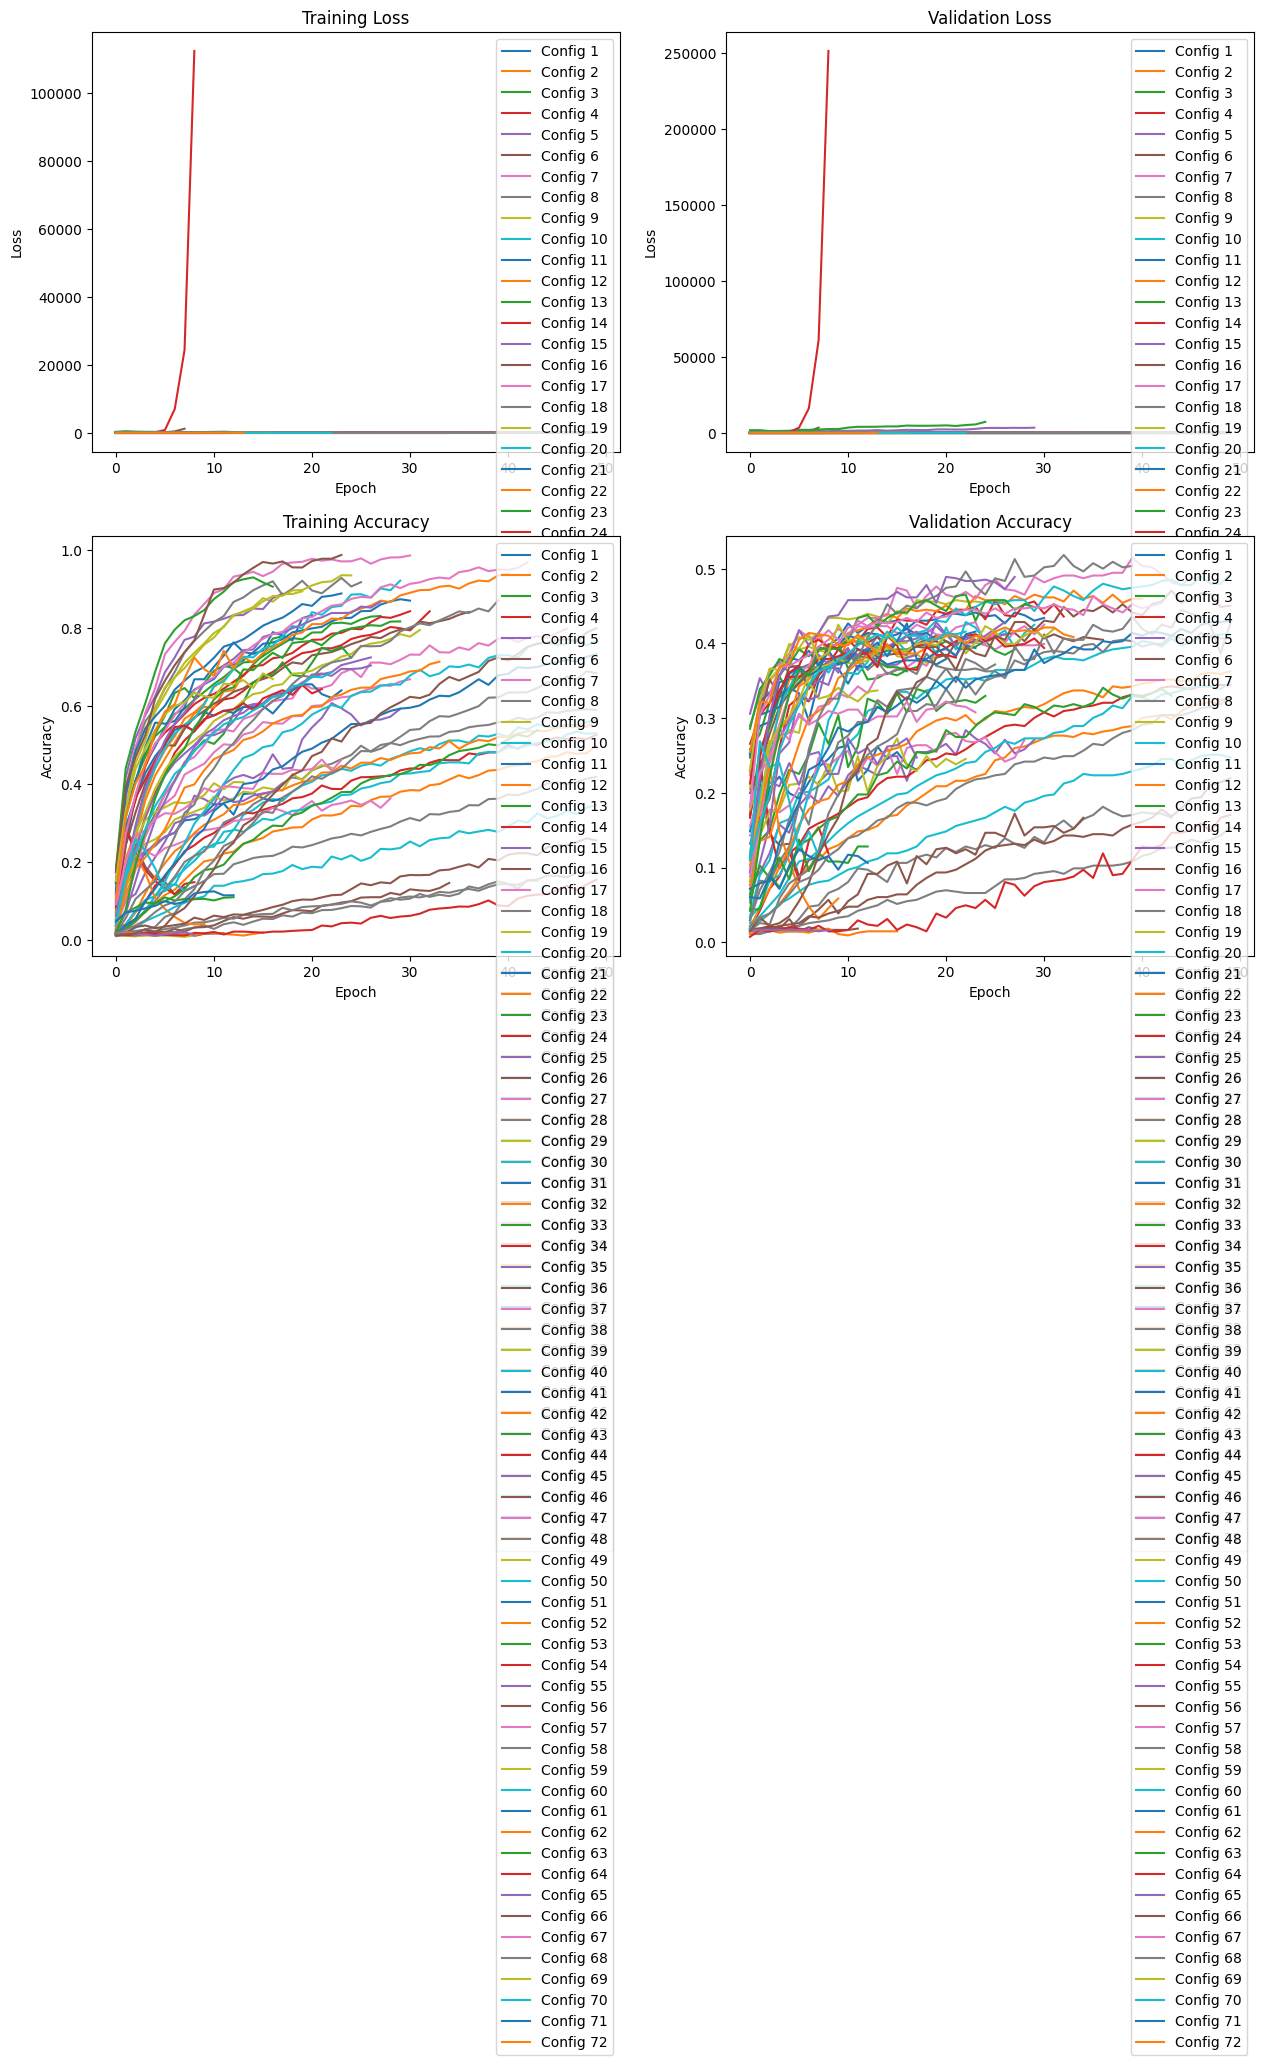
\includegraphics[width=469.5pt,height=767.0233pt]{latexImage_c7a4da05350858359df32b329dc5177f.png}}
\end{picture}
\newpage
\begin{tikzpicture}[overlay]
\path(0pt,0pt);
\filldraw[color_283006][even odd rule]
(21pt, -746pt) -- (561pt, -746pt)
 -- (561pt, -746pt)
 -- (561pt, -26pt)
 -- (561pt, -26pt)
 -- (21pt, -26pt) -- cycle
;
\filldraw[color_273076][even odd rule]
(89.25pt, -725.4967pt) -- (549.75pt, -725.4967pt)
 -- (549.75pt, -725.4967pt)
 -- (549.75pt, -525.2456pt)
 -- (549.75pt, -525.2456pt)
 -- (89.25pt, -525.2456pt) -- cycle
;
\filldraw[color_252223][nonzero rule]
(89.25pt, -725.4967pt) -- (89.25pt, -525.2456pt)
 -- (89.25pt, -525.2456pt)
 -- (549.75pt, -525.2456pt)
 -- (549.75pt, -525.2456pt)
 -- (549.75pt, -725.4967pt)
 -- (549.75pt, -725.4967pt)
 -- (549pt, -725.4967pt)
 -- (549pt, -725.4967pt)
 -- (549pt, -525.9956pt)
 -- (549pt, -525.9956pt)
 -- (90pt, -525.9956pt)
 -- (90pt, -525.9956pt)
 -- (90pt, -725.4967pt) -- cycle
;
\begin{scope}
\clip
(32.25pt, -725.4967pt) -- (549.75pt, -725.4967pt)
 -- (549.75pt, -725.4967pt)
 -- (549.75pt, -525.2456pt)
 -- (549.75pt, -525.2456pt)
 -- (32.25pt, -525.2456pt) -- cycle
;
\begin{scope}
\clip
(90pt, -724.7467pt) -- (549pt, -724.7467pt)
 -- (549pt, -724.7467pt)
 -- (549pt, -525.9956pt)
 -- (549pt, -525.9956pt)
 -- (90pt, -525.9956pt) -- cycle
;
\filldraw[color_273076][even odd rule]
(90pt, -724.7467pt) -- (549pt, -724.7467pt)
 -- (549pt, -724.7467pt)
 -- (549pt, -525.9956pt)
 -- (549pt, -525.9956pt)
 -- (90pt, -525.9956pt) -- cycle
;
\end{scope}
\end{scope}
\begin{scope}
\clip
(32.25pt, -466.7pt) -- (549.75pt, -466.7pt)
 -- (549.75pt, -466.7pt)
 -- (549.75pt, -37.25pt)
 -- (549.75pt, -37.25pt)
 -- (32.25pt, -37.25pt) -- cycle
;
\end{scope}
\end{tikzpicture}
\begin{picture}(-5,0)(2.5,0)
\put(93,-49.28497){\fontsize{10.5}{1}\usefont{T1}{cmr}{b}{n}\selectfont\color{color_29791}Best Model Justification: [256, 128], ReLU, LR=0.01, SGD}
\put(93,-76.58502){\fontsize{10.5}{1}\usefont{T1}{cmr}{m}{n}\selectfont\color{color_29791}✓Highest Accuracy: 50.37\% validation accuracy (best overall)}
\put(93,-103.885){\fontsize{10.5}{1}\usefont{T1}{cmr}{m}{n}\selectfont\color{color_29791}✓Optimal Architecture:}
\put(139.8066,-132.445){\fontsize{10.5}{1}\usefont{T1}{cmr}{m}{n}\selectfont\color{color_29791}•Two hidden layers provide right complexity}
\put(139.8066,-149.245){\fontsize{10.5}{1}\usefont{T1}{cmr}{m}{n}\selectfont\color{color_29791}•256→128 nodes balance capacity and efiiciency}
\put(93,-176.545){\fontsize{10.5}{1}\usefont{T1}{cmr}{m}{n}\selectfont\color{color_29791}✓ReLU Superiority:}
\put(139.8066,-205.105){\fontsize{10.5}{1}\usefont{T1}{cmr}{m}{n}\selectfont\color{color_29791}•Faster convergence than sigmoid/tanh}
\put(139.8066,-221.905){\fontsize{10.5}{1}\usefont{T1}{cmr}{m}{n}\selectfont\color{color_29791}•Better for image data}
\put(93,-249.205){\fontsize{10.5}{1}\usefont{T1}{cmr}{m}{n}\selectfont\color{color_29791}✓SGD Advantage:}
\put(139.8066,-277.765){\fontsize{10.5}{1}\usefont{T1}{cmr}{m}{n}\selectfont\color{color_29791}•Better generalization than Adam for this task}
\put(139.8066,-294.565){\fontsize{10.5}{1}\usefont{T1}{cmr}{m}{n}\selectfont\color{color_29791}•Stable with momentum (0.9)}
\put(93,-321.865){\fontsize{10.5}{1}\usefont{T1}{cmr}{m}{n}\selectfont\color{color_29791}✓Ideal Learning Rate:}
\put(139.8066,-350.425){\fontsize{10.5}{1}\usefont{T1}{cmr}{m}{n}\selectfont\color{color_29791}•0.01 balanced speed and stability}
\put(139.8066,-367.225){\fontsize{10.5}{1}\usefont{T1}{cmr}{m}{n}\selectfont\color{color_29791}•Avoided divergence (high LR) and slow training (low LR)}
\put(93,-394.525){\fontsize{10.5}{1}\usefont{T1}{cmr}{m}{n}\selectfont\color{color_29791}✓Proven Performance:}
\put(139.8066,-423.085){\fontsize{10.5}{1}\usefont{T1}{cmr}{m}{n}\selectfont\color{color_29791}•Consistently improved over 40 epochs}
\put(139.8066,-439.885){\fontsize{10.5}{1}\usefont{T1}{cmr}{m}{n}\selectfont\color{color_29791}•No overfitting issues}
\put(139.8066,-456.685){\fontsize{10.5}{1}\usefont{T1}{cmr}{m}{n}\selectfont\color{color_29791}•Outperformed all other configurations}
\put(93,-505.6876){\fontsize{21.7728}{1}\usefont{T1}{cmr}{b}{n}\selectfont\color{color_29791}5.PLA AND MLP COMPARISON}
\put(93,-539.496){\fontsize{9.75}{1}\usefont{T1}{cmr}{m}{n}\selectfont\color{color_95391}\# Train the best model with more epochs if needed}
\put(93,-552.2461){\fontsize{9.75}{1}\usefont{T1}{cmr}{m}{n}\selectfont\color{color_62560}print("Training best model with optimal parameters...")}
\put(93,-577.7462){\fontsize{9.75}{1}\usefont{T1}{cmr}{m}{n}\selectfont\color{color_95391}\# Reinitialize best model with best parameters}
\put(93,-590.4963){\fontsize{9.75}{1}\usefont{T1}{cmr}{m}{n}\selectfont\color{color_62560}final\_model=MLP(}
\put(116.48,-603.2464){\fontsize{9.75}{1}\usefont{T1}{cmr}{m}{n}\selectfont\color{color_62560}input\_size,}
\put(116.48,-615.9965){\fontsize{9.75}{1}\usefont{T1}{cmr}{m}{n}\selectfont\color{color_62560}best\_params['hidden\_layers'],}
\put(116.48,-628.7465){\fontsize{9.75}{1}\usefont{T1}{cmr}{m}{n}\selectfont\color{color_62560}num\_classes,}
\put(116.48,-641.4966){\fontsize{9.75}{1}\usefont{T1}{cmr}{m}{n}\selectfont\color{color_62560}activation=best\_params['activation']}
\put(93,-654.2467){\fontsize{9.75}{1}\usefont{T1}{cmr}{m}{n}\selectfont\color{color_32596})}
\put(93,-679.7468){\fontsize{9.75}{1}\usefont{T1}{cmr}{m}{n}\selectfont\color{color_62560}criterion=nn.CrossEntropyLoss()}
\put(93,-705.247){\fontsize{9.75}{1}\usefont{T1}{cmr}{b}{n}\selectfont\color{color_33759}ifbest\_params['optimizer']=='adam':}
\put(116.48,-717.9971){\fontsize{9.75}{1}\usefont{T1}{cmr}{m}{n}\selectfont\color{color_62560}optimizer=optim.Adam(final\_model.parameters(),lr=best\_params['learning\_rate'}
\put(43.66,-539.496){\fontsize{9.75}{1}\usefont{T1}{cmr}{m}{n}\selectfont\color{color_126112}In[9]:}
\end{picture}
\newpage
\begin{tikzpicture}[overlay]
\path(0pt,0pt);
\filldraw[color_283006][even odd rule]
(21pt, -746pt) -- (561pt, -746pt)
 -- (561pt, -746pt)
 -- (561pt, -26pt)
 -- (561pt, -26pt)
 -- (21pt, -26pt) -- cycle
;
\filldraw[color_273076][even odd rule]
(89.25pt, -722.004pt) -- (549.75pt, -722.004pt)
 -- (549.75pt, -722.004pt)
 -- (549.75pt, -37.25pt)
 -- (549.75pt, -37.25pt)
 -- (89.25pt, -37.25pt) -- cycle
;
\filldraw[color_252223][nonzero rule]
(89.25pt, -722.004pt) -- (90pt, -722.004pt)
 -- (90pt, -722.004pt)
 -- (90pt, -37.25pt)
 -- (90pt, -37.25pt)
 -- (89.25pt, -37.25pt) -- cycle
;
\filldraw[color_252223][nonzero rule]
(549pt, -722.004pt) -- (549.75pt, -722.004pt)
 -- (549.75pt, -722.004pt)
 -- (549.75pt, -37.25pt)
 -- (549.75pt, -37.25pt)
 -- (549pt, -37.25pt) -- cycle
;
\begin{scope}
\clip
(32.25pt, -722.004pt) -- (549.75pt, -722.004pt)
 -- (549.75pt, -722.004pt)
 -- (549.75pt, -37.25pt)
 -- (549.75pt, -37.25pt)
 -- (32.25pt, -37.25pt) -- cycle
;
\begin{scope}
\clip
(90pt, -721.254pt) -- (549pt, -721.254pt)
 -- (549pt, -721.254pt)
 -- (549pt, -38pt)
 -- (549pt, -38pt)
 -- (90pt, -38pt) -- cycle
;
\filldraw[color_273076][even odd rule]
(90pt, -721.254pt) -- (549pt, -721.254pt)
 -- (549pt, -721.254pt)
 -- (549pt, -38pt)
 -- (549pt, -38pt)
 -- (90pt, -38pt) -- cycle
;
\end{scope}
\end{scope}
\begin{scope}
\clip
(32.25pt, -722.004pt) -- (549.75pt, -722.004pt)
 -- (549.75pt, -722.004pt)
 -- (549.75pt, -37.25pt)
 -- (549.75pt, -37.25pt)
 -- (32.25pt, -37.25pt) -- cycle
;
\begin{scope}
\clip
(90pt, -721.254pt) -- (549pt, -721.254pt)
 -- (549pt, -721.254pt)
 -- (549pt, -38pt)
 -- (549pt, -38pt)
 -- (90pt, -38pt) -- cycle
;
\end{scope}
\end{scope}
\end{tikzpicture}
\begin{picture}(-5,0)(2.5,0)
\put(93,-51.50043){\fontsize{9.75}{1}\usefont{T1}{cmr}{b}{n}\selectfont\color{color_33759}else:}
\put(116.48,-64.25049){\fontsize{9.75}{1}\usefont{T1}{cmr}{m}{n}\selectfont\color{color_62560}optimizer=optim.SGD(final\_model.parameters(),lr=best\_params['learning\_rate'}
\put(93,-89.75061){\fontsize{9.75}{1}\usefont{T1}{cmr}{m}{n}\selectfont\color{color_95391}\# Train the model}
\put(93,-102.5007){\fontsize{9.75}{1}\usefont{T1}{cmr}{m}{n}\selectfont\color{color_62560}final\_model,train\_losses,val\_losses,train\_accs,val\_accs=train\_model(}
\put(116.48,-115.2508){\fontsize{9.75}{1}\usefont{T1}{cmr}{m}{n}\selectfont\color{color_62560}final\_model,train\_loader,val\_loader,criterion,optimizer,}
\put(116.48,-128.0009){\fontsize{9.75}{1}\usefont{T1}{cmr}{m}{n}\selectfont\color{color_62560}num\_epochs=100,patience=10}
\put(93,-140.7509){\fontsize{9.75}{1}\usefont{T1}{cmr}{m}{n}\selectfont\color{color_32596})}
\put(93,-166.2511){\fontsize{9.75}{1}\usefont{T1}{cmr}{m}{n}\selectfont\color{color_95391}\# Plot training history}
\put(93,-179.0012){\fontsize{9.75}{1}\usefont{T1}{cmr}{m}{n}\selectfont\color{color_62560}plt.figure(figsize=(15,5))}
\put(93,-204.5013){\fontsize{9.75}{1}\usefont{T1}{cmr}{m}{n}\selectfont\color{color_62560}plt.subplot(1,3,1)}
\put(93,-217.2514){\fontsize{9.75}{1}\usefont{T1}{cmr}{m}{n}\selectfont\color{color_62560}plt.plot(train\_losses,label='Training Loss')}
\put(93,-230.0015){\fontsize{9.75}{1}\usefont{T1}{cmr}{m}{n}\selectfont\color{color_62560}plt.plot(val\_losses,label='Validation Loss')}
\put(93,-242.7515){\fontsize{9.75}{1}\usefont{T1}{cmr}{m}{n}\selectfont\color{color_62560}plt.title('Training and Validation Loss')}
\put(93,-255.5016){\fontsize{9.75}{1}\usefont{T1}{cmr}{m}{n}\selectfont\color{color_62560}plt.xlabel('Epochs')}
\put(93,-268.2517){\fontsize{9.75}{1}\usefont{T1}{cmr}{m}{n}\selectfont\color{color_62560}plt.ylabel('Loss')}
\put(93,-281.0018){\fontsize{9.75}{1}\usefont{T1}{cmr}{m}{n}\selectfont\color{color_62560}plt.legend()}
\put(93,-306.5019){\fontsize{9.75}{1}\usefont{T1}{cmr}{m}{n}\selectfont\color{color_62560}plt.subplot(1,3,2)}
\put(93,-319.252){\fontsize{9.75}{1}\usefont{T1}{cmr}{m}{n}\selectfont\color{color_62560}plt.plot(train\_accs,label='Training Accuracy')}
\put(93,-332.0021){\fontsize{9.75}{1}\usefont{T1}{cmr}{m}{n}\selectfont\color{color_62560}plt.plot(val\_accs,label='Validation Accuracy')}
\put(93,-344.7521){\fontsize{9.75}{1}\usefont{T1}{cmr}{m}{n}\selectfont\color{color_62560}plt.title('Training and Validation Accuracy')}
\put(93,-357.5022){\fontsize{9.75}{1}\usefont{T1}{cmr}{m}{n}\selectfont\color{color_62560}plt.xlabel('Epochs')}
\put(93,-370.2523){\fontsize{9.75}{1}\usefont{T1}{cmr}{m}{n}\selectfont\color{color_62560}plt.ylabel('Accuracy')}
\put(93,-383.0024){\fontsize{9.75}{1}\usefont{T1}{cmr}{m}{n}\selectfont\color{color_62560}plt.legend()}
\put(93,-408.5025){\fontsize{9.75}{1}\usefont{T1}{cmr}{m}{n}\selectfont\color{color_95391}\# Plot learning curve (accuracy vs loss)}
\put(93,-421.2526){\fontsize{9.75}{1}\usefont{T1}{cmr}{m}{n}\selectfont\color{color_62560}plt.subplot(1,3,3)}
\put(93,-434.0027){\fontsize{9.75}{1}\usefont{T1}{cmr}{m}{n}\selectfont\color{color_62560}plt.plot(train\_losses,train\_accs,'o-',label='Training')}
\put(93,-446.7527){\fontsize{9.75}{1}\usefont{T1}{cmr}{m}{n}\selectfont\color{color_62560}plt.plot(val\_losses,val\_accs,'o-',label='Validation')}
\put(93,-459.5028){\fontsize{9.75}{1}\usefont{T1}{cmr}{m}{n}\selectfont\color{color_62560}plt.title('Learning Curve')}
\put(93,-472.2529){\fontsize{9.75}{1}\usefont{T1}{cmr}{m}{n}\selectfont\color{color_62560}plt.xlabel('Loss')}
\put(93,-485.003){\fontsize{9.75}{1}\usefont{T1}{cmr}{m}{n}\selectfont\color{color_62560}plt.ylabel('Accuracy')}
\put(93,-497.753){\fontsize{9.75}{1}\usefont{T1}{cmr}{m}{n}\selectfont\color{color_62560}plt.legend()}
\put(93,-523.2532){\fontsize{9.75}{1}\usefont{T1}{cmr}{m}{n}\selectfont\color{color_62560}plt.tight\_layout()}
\put(93,-536.0033){\fontsize{9.75}{1}\usefont{T1}{cmr}{m}{n}\selectfont\color{color_62560}plt.show()}
\put(93,-561.5034){\fontsize{9.75}{1}\usefont{T1}{cmr}{m}{n}\selectfont\color{color_95391}\# Evaluate on test set}
\put(93,-574.2535){\fontsize{9.75}{1}\usefont{T1}{cmr}{m}{n}\selectfont\color{color_62560}mlp\_test\_acc,mlp\_preds,mlp\_true,mlp\_probs=evaluate\_model(final\_model,test\_loader}
\put(93,-587.0036){\fontsize{9.75}{1}\usefont{T1}{cmr}{m}{n}\selectfont\color{color_62560}mlp\_precision=precision\_score(mlp\_true,mlp\_preds,average='weighted',zero\_division}
\put(93,-599.7536){\fontsize{9.75}{1}\usefont{T1}{cmr}{m}{n}\selectfont\color{color_62560}mlp\_recall=recall\_score(mlp\_true,mlp\_preds,average='weighted',zero\_division}
\put(93,-612.5037){\fontsize{9.75}{1}\usefont{T1}{cmr}{m}{n}\selectfont\color{color_62560}mlp\_f1=f1\_score(mlp\_true,mlp\_preds,average='weighted',zero\_division=0)}
\put(93,-638.0039){\fontsize{9.75}{1}\usefont{T1}{cmr}{m}{n}\selectfont\color{color_62560}print(f"MLP Test Accuracy:\{mlp\_test\_acc:.4f\}")}
\put(93,-650.7539){\fontsize{9.75}{1}\usefont{T1}{cmr}{m}{n}\selectfont\color{color_62560}print(f"MLP Test Precision:\{mlp\_precision:.4f\}")}
\put(93,-663.504){\fontsize{9.75}{1}\usefont{T1}{cmr}{m}{n}\selectfont\color{color_62560}print(f"MLP Test Recall:\{mlp\_recall:.4f\}")}
\put(93,-676.2541){\fontsize{9.75}{1}\usefont{T1}{cmr}{m}{n}\selectfont\color{color_62560}print(f"MLP Test F1-Score:\{mlp\_f1:.4f\}")}
\put(93,-701.7542){\fontsize{9.75}{1}\usefont{T1}{cmr}{m}{n}\selectfont\color{color_95391}\# Compare with PLA}
\put(93,-714.5043){\fontsize{9.75}{1}\usefont{T1}{cmr}{m}{n}\selectfont\color{color_62560}print("\n=== Model Comparison ===")}
\end{picture}
\newpage
\begin{tikzpicture}[overlay]
\path(0pt,0pt);
\filldraw[color_283006][even odd rule]
(21pt, -746pt) -- (561pt, -746pt)
 -- (561pt, -746pt)
 -- (561pt, -26pt)
 -- (561pt, -26pt)
 -- (21pt, -26pt) -- cycle
;
\filldraw[color_273076][even odd rule]
(89.25pt, -722.004pt) -- (549.75pt, -722.004pt)
 -- (549.75pt, -722.004pt)
 -- (549.75pt, -37.25pt)
 -- (549.75pt, -37.25pt)
 -- (89.25pt, -37.25pt) -- cycle
;
\filldraw[color_252223][nonzero rule]
(89.25pt, -722.004pt) -- (90pt, -722.004pt)
 -- (90pt, -722.004pt)
 -- (90pt, -37.25pt)
 -- (90pt, -37.25pt)
 -- (89.25pt, -37.25pt) -- cycle
;
\filldraw[color_252223][nonzero rule]
(549pt, -722.004pt) -- (549.75pt, -722.004pt)
 -- (549.75pt, -722.004pt)
 -- (549.75pt, -37.25pt)
 -- (549.75pt, -37.25pt)
 -- (549pt, -37.25pt) -- cycle
;
\begin{scope}
\clip
(32.25pt, -722.004pt) -- (549.75pt, -722.004pt)
 -- (549.75pt, -722.004pt)
 -- (549.75pt, -37.25pt)
 -- (549.75pt, -37.25pt)
 -- (32.25pt, -37.25pt) -- cycle
;
\begin{scope}
\clip
(90pt, -721.254pt) -- (549pt, -721.254pt)
 -- (549pt, -721.254pt)
 -- (549pt, -38pt)
 -- (549pt, -38pt)
 -- (90pt, -38pt) -- cycle
;
\filldraw[color_273076][even odd rule]
(90pt, -721.254pt) -- (549pt, -721.254pt)
 -- (549pt, -721.254pt)
 -- (549pt, -38pt)
 -- (549pt, -38pt)
 -- (90pt, -38pt) -- cycle
;
\end{scope}
\end{scope}
\begin{scope}
\clip
(32.25pt, -722.004pt) -- (549.75pt, -722.004pt)
 -- (549.75pt, -722.004pt)
 -- (549.75pt, -37.25pt)
 -- (549.75pt, -37.25pt)
 -- (32.25pt, -37.25pt) -- cycle
;
\begin{scope}
\clip
(90pt, -721.254pt) -- (549pt, -721.254pt)
 -- (549pt, -721.254pt)
 -- (549pt, -38pt)
 -- (549pt, -38pt)
 -- (90pt, -38pt) -- cycle
;
\end{scope}
\end{scope}
\end{tikzpicture}
\begin{picture}(-5,0)(2.5,0)
\put(93,-51.50043){\fontsize{9.75}{1}\usefont{T1}{cmr}{m}{n}\selectfont\color{color_62560}print(f"PLA Test Accuracy:\{pla\_accuracy:.4f\}")}
\put(93,-64.25049){\fontsize{9.75}{1}\usefont{T1}{cmr}{m}{n}\selectfont\color{color_62560}print(f"MLP Test Accuracy:\{mlp\_test\_acc:.4f\}")}
\put(93,-77.00061){\fontsize{9.75}{1}\usefont{T1}{cmr}{m}{n}\selectfont\color{color_62560}print(f"Improvement:\{(mlp\_test\_acc-pla\_accuracy)*100:.2f\}\%")}
\put(93,-102.5007){\fontsize{9.75}{1}\usefont{T1}{cmr}{m}{n}\selectfont\color{color_95391}\# Confusion matrix for both models}
\put(93,-115.2508){\fontsize{9.75}{1}\usefont{T1}{cmr}{m}{n}\selectfont\color{color_62560}fig,axes=plt.subplots(1,2,figsize=(15,6))}
\put(93,-140.7509){\fontsize{9.75}{1}\usefont{T1}{cmr}{m}{n}\selectfont\color{color_95391}\# PLA confusion matrix}
\put(93,-153.501){\fontsize{9.75}{1}\usefont{T1}{cmr}{m}{n}\selectfont\color{color_62560}cm\_pla=confusion\_matrix(y\_test,y\_pred\_pla)}
\put(93,-166.2511){\fontsize{9.75}{1}\usefont{T1}{cmr}{m}{n}\selectfont\color{color_62560}sns.heatmap(cm\_pla,annot=False,fmt='d',cmap='Blues',ax=axes[0])}
\put(93,-179.0012){\fontsize{9.75}{1}\usefont{T1}{cmr}{m}{n}\selectfont\color{color_62560}axes[0].set\_title('PLA Confusion Matrix')}
\put(93,-191.7512){\fontsize{9.75}{1}\usefont{T1}{cmr}{m}{n}\selectfont\color{color_62560}axes[0].set\_ylabel('True Label')}
\put(93,-204.5013){\fontsize{9.75}{1}\usefont{T1}{cmr}{m}{n}\selectfont\color{color_62560}axes[0].set\_xlabel('Predicted Label')}
\put(93,-230.0015){\fontsize{9.75}{1}\usefont{T1}{cmr}{m}{n}\selectfont\color{color_95391}\# MLP confusion matrix}
\put(93,-242.7515){\fontsize{9.75}{1}\usefont{T1}{cmr}{m}{n}\selectfont\color{color_62560}cm\_mlp=confusion\_matrix(mlp\_true,mlp\_preds)}
\put(93,-255.5016){\fontsize{9.75}{1}\usefont{T1}{cmr}{m}{n}\selectfont\color{color_62560}sns.heatmap(cm\_mlp,annot=False,fmt='d',cmap='Blues',ax=axes[1])}
\put(93,-268.2517){\fontsize{9.75}{1}\usefont{T1}{cmr}{m}{n}\selectfont\color{color_62560}axes[1].set\_title('MLP Confusion Matrix')}
\put(93,-281.0018){\fontsize{9.75}{1}\usefont{T1}{cmr}{m}{n}\selectfont\color{color_62560}axes[1].set\_ylabel('True Label')}
\put(93,-293.7518){\fontsize{9.75}{1}\usefont{T1}{cmr}{m}{n}\selectfont\color{color_62560}axes[1].set\_xlabel('Predicted Label')}
\put(93,-319.252){\fontsize{9.75}{1}\usefont{T1}{cmr}{m}{n}\selectfont\color{color_62560}plt.tight\_layout()}
\put(93,-332.0021){\fontsize{9.75}{1}\usefont{T1}{cmr}{m}{n}\selectfont\color{color_62560}plt.show()}
\put(93,-357.5022){\fontsize{9.75}{1}\usefont{T1}{cmr}{m}{n}\selectfont\color{color_95391}\# ROC Curves}
\put(93,-370.2523){\fontsize{9.75}{1}\usefont{T1}{cmr}{m}{n}\selectfont\color{color_95391}\# Binarize the output for ROC curve}
\put(93,-383.0024){\fontsize{9.75}{1}\usefont{T1}{cmr}{m}{n}\selectfont\color{color_62560}y\_test\_bin=label\_binarize(y\_test,classes=np.arange(num\_classes))}
\put(93,-395.7524){\fontsize{9.75}{1}\usefont{T1}{cmr}{m}{n}\selectfont\color{color_62560}y\_test\_bin\_mlp=label\_binarize(mlp\_true,classes=np.arange(num\_classes))}
\put(93,-421.2526){\fontsize{9.75}{1}\usefont{T1}{cmr}{m}{n}\selectfont\color{color_95391}\# Compute ROC curve and ROC area for each class for PLA}
\put(93,-434.0027){\fontsize{9.75}{1}\usefont{T1}{cmr}{m}{n}\selectfont\color{color_62560}fpr\_pla=dict()}
\put(93,-446.7527){\fontsize{9.75}{1}\usefont{T1}{cmr}{m}{n}\selectfont\color{color_62560}tpr\_pla=dict()}
\put(93,-459.5028){\fontsize{9.75}{1}\usefont{T1}{cmr}{m}{n}\selectfont\color{color_62560}roc\_auc\_pla=dict()}
\put(93,-485.003){\fontsize{9.75}{1}\usefont{T1}{cmr}{b}{n}\selectfont\color{color_33759}foriinrange(num\_classes):}
\put(116.48,-497.753){\fontsize{9.75}{1}\usefont{T1}{cmr}{m}{n}\selectfont\color{color_62560}fpr\_pla[i],tpr\_pla[i],\_=roc\_curve(y\_test\_bin[:,i],y\_proba\_pla[:,i])}
\put(116.48,-510.5031){\fontsize{9.75}{1}\usefont{T1}{cmr}{m}{n}\selectfont\color{color_62560}roc\_auc\_pla[i]=auc(fpr\_pla[i],tpr\_pla[i])}
\put(93,-536.0033){\fontsize{9.75}{1}\usefont{T1}{cmr}{m}{n}\selectfont\color{color_95391}\# Compute micro-average ROC curve and ROC area for PLA}
\put(93,-548.7533){\fontsize{9.75}{1}\usefont{T1}{cmr}{m}{n}\selectfont\color{color_62560}fpr\_pla["micro"],tpr\_pla["micro"],\_=roc\_curve(y\_test\_bin.ravel(),y\_proba\_pla}
\put(93,-561.5034){\fontsize{9.75}{1}\usefont{T1}{cmr}{m}{n}\selectfont\color{color_62560}roc\_auc\_pla["micro"]=auc(fpr\_pla["micro"],tpr\_pla["micro"])}
\put(93,-587.0036){\fontsize{9.75}{1}\usefont{T1}{cmr}{m}{n}\selectfont\color{color_95391}\# Compute ROC curve and ROC area for each class for MLP}
\put(93,-599.7536){\fontsize{9.75}{1}\usefont{T1}{cmr}{m}{n}\selectfont\color{color_62560}fpr\_mlp=dict()}
\put(93,-612.5037){\fontsize{9.75}{1}\usefont{T1}{cmr}{m}{n}\selectfont\color{color_62560}tpr\_mlp=dict()}
\put(93,-625.2538){\fontsize{9.75}{1}\usefont{T1}{cmr}{m}{n}\selectfont\color{color_62560}roc\_auc\_mlp=dict()}
\put(93,-650.7539){\fontsize{9.75}{1}\usefont{T1}{cmr}{b}{n}\selectfont\color{color_33759}foriinrange(num\_classes):}
\put(116.48,-663.504){\fontsize{9.75}{1}\usefont{T1}{cmr}{m}{n}\selectfont\color{color_62560}fpr\_mlp[i],tpr\_mlp[i],\_=roc\_curve(y\_test\_bin\_mlp[:,i],mlp\_probs[:,i])}
\put(116.48,-676.2541){\fontsize{9.75}{1}\usefont{T1}{cmr}{m}{n}\selectfont\color{color_62560}roc\_auc\_mlp[i]=auc(fpr\_mlp[i],tpr\_mlp[i])}
\put(93,-701.7542){\fontsize{9.75}{1}\usefont{T1}{cmr}{m}{n}\selectfont\color{color_95391}\# Compute micro-average ROC curve and ROC area for MLP}
\put(93,-714.5043){\fontsize{9.75}{1}\usefont{T1}{cmr}{m}{n}\selectfont\color{color_62560}fpr\_mlp["micro"],tpr\_mlp["micro"],\_=roc\_curve(y\_test\_bin\_mlp.ravel(),mlp\_probs}
\end{picture}
\newpage
\begin{tikzpicture}[overlay]
\path(0pt,0pt);
\filldraw[color_283006][even odd rule]
(21pt, -746pt) -- (561pt, -746pt)
 -- (561pt, -746pt)
 -- (561pt, -26pt)
 -- (561pt, -26pt)
 -- (21pt, -26pt) -- cycle
;
\filldraw[color_273076][even odd rule]
(89.25pt, -722.004pt) -- (549.75pt, -722.004pt)
 -- (549.75pt, -722.004pt)
 -- (549.75pt, -37.25pt)
 -- (549.75pt, -37.25pt)
 -- (89.25pt, -37.25pt) -- cycle
;
\filldraw[color_252223][nonzero rule]
(89.25pt, -722.004pt) -- (90pt, -722.004pt)
 -- (90pt, -722.004pt)
 -- (90pt, -37.25pt)
 -- (90pt, -37.25pt)
 -- (89.25pt, -37.25pt) -- cycle
;
\filldraw[color_252223][nonzero rule]
(549pt, -722.004pt) -- (549.75pt, -722.004pt)
 -- (549.75pt, -722.004pt)
 -- (549.75pt, -37.25pt)
 -- (549.75pt, -37.25pt)
 -- (549pt, -37.25pt) -- cycle
;
\begin{scope}
\clip
(32.25pt, -722.004pt) -- (549.75pt, -722.004pt)
 -- (549.75pt, -722.004pt)
 -- (549.75pt, -37.25pt)
 -- (549.75pt, -37.25pt)
 -- (32.25pt, -37.25pt) -- cycle
;
\begin{scope}
\clip
(90pt, -721.254pt) -- (549pt, -721.254pt)
 -- (549pt, -721.254pt)
 -- (549pt, -38pt)
 -- (549pt, -38pt)
 -- (90pt, -38pt) -- cycle
;
\filldraw[color_273076][even odd rule]
(90pt, -721.254pt) -- (549pt, -721.254pt)
 -- (549pt, -721.254pt)
 -- (549pt, -38pt)
 -- (549pt, -38pt)
 -- (90pt, -38pt) -- cycle
;
\end{scope}
\end{scope}
\begin{scope}
\clip
(32.25pt, -722.004pt) -- (549.75pt, -722.004pt)
 -- (549.75pt, -722.004pt)
 -- (549.75pt, -37.25pt)
 -- (549.75pt, -37.25pt)
 -- (32.25pt, -37.25pt) -- cycle
;
\begin{scope}
\clip
(90pt, -721.254pt) -- (549pt, -721.254pt)
 -- (549pt, -721.254pt)
 -- (549pt, -38pt)
 -- (549pt, -38pt)
 -- (90pt, -38pt) -- cycle
;
\end{scope}
\end{scope}
\end{tikzpicture}
\begin{picture}(-5,0)(2.5,0)
\put(93,-51.50043){\fontsize{9.75}{1}\usefont{T1}{cmr}{m}{n}\selectfont\color{color_62560}roc\_auc\_mlp["micro"]=auc(fpr\_mlp["micro"],tpr\_mlp["micro"])}
\put(93,-77.00061){\fontsize{9.75}{1}\usefont{T1}{cmr}{m}{n}\selectfont\color{color_95391}\# Plot ROC curves}
\put(93,-89.75061){\fontsize{9.75}{1}\usefont{T1}{cmr}{m}{n}\selectfont\color{color_62560}plt.figure(figsize=(12,5))}
\put(93,-115.2508){\fontsize{9.75}{1}\usefont{T1}{cmr}{m}{n}\selectfont\color{color_62560}plt.subplot(1,2,1)}
\put(93,-128.0009){\fontsize{9.75}{1}\usefont{T1}{cmr}{m}{n}\selectfont\color{color_62560}plt.plot(fpr\_pla["micro"],tpr\_pla["micro"],}
\put(145.83,-140.7509){\fontsize{9.75}{1}\usefont{T1}{cmr}{m}{n}\selectfont\color{color_62560}label='PLA micro-average ROC curve (area =\{0:0.2f\})'}
\put(181.0499,-153.501){\fontsize{9.75}{1}\usefont{T1}{cmr}{m}{n}\selectfont\color{color_209593}''.format(roc\_auc\_pla["micro"]),}
\put(145.83,-166.2511){\fontsize{9.75}{1}\usefont{T1}{cmr}{m}{n}\selectfont\color{color_62560}color='deeppink',linestyle=':',linewidth=4)}
\put(93,-191.7512){\fontsize{9.75}{1}\usefont{T1}{cmr}{m}{n}\selectfont\color{color_62560}plt.plot(fpr\_mlp["micro"],tpr\_mlp["micro"],}
\put(145.83,-204.5013){\fontsize{9.75}{1}\usefont{T1}{cmr}{m}{n}\selectfont\color{color_62560}label='MLP micro-average ROC curve (area =\{0:0.2f\})'}
\put(181.0499,-217.2514){\fontsize{9.75}{1}\usefont{T1}{cmr}{m}{n}\selectfont\color{color_209593}''.format(roc\_auc\_mlp["micro"]),}
\put(145.83,-230.0015){\fontsize{9.75}{1}\usefont{T1}{cmr}{m}{n}\selectfont\color{color_62560}color='navy',linestyle=':',linewidth=4)}
\put(93,-255.5016){\fontsize{9.75}{1}\usefont{T1}{cmr}{m}{n}\selectfont\color{color_62560}plt.plot([0,1],[0,1],'k--',lw=2)}
\put(93,-268.2517){\fontsize{9.75}{1}\usefont{T1}{cmr}{m}{n}\selectfont\color{color_62560}plt.xlim([0.0,1.0])}
\put(93,-281.0018){\fontsize{9.75}{1}\usefont{T1}{cmr}{m}{n}\selectfont\color{color_62560}plt.ylim([0.0,1.05])}
\put(93,-293.7518){\fontsize{9.75}{1}\usefont{T1}{cmr}{m}{n}\selectfont\color{color_62560}plt.xlabel('False Positive Rate')}
\put(93,-306.5019){\fontsize{9.75}{1}\usefont{T1}{cmr}{m}{n}\selectfont\color{color_62560}plt.ylabel('True Positive Rate')}
\put(93,-319.252){\fontsize{9.75}{1}\usefont{T1}{cmr}{m}{n}\selectfont\color{color_62560}plt.title('Micro-average ROC Curve')}
\put(93,-332.0021){\fontsize{9.75}{1}\usefont{T1}{cmr}{m}{n}\selectfont\color{color_62560}plt.legend(loc="lower right")}
\put(93,-357.5022){\fontsize{9.75}{1}\usefont{T1}{cmr}{m}{n}\selectfont\color{color_95391}\# Macro-average ROC curve}
\put(93,-370.2523){\fontsize{9.75}{1}\usefont{T1}{cmr}{m}{n}\selectfont\color{color_95391}\# First aggregate all false positive rates}
\put(93,-383.0024){\fontsize{9.75}{1}\usefont{T1}{cmr}{m}{n}\selectfont\color{color_62560}all\_fpr\_pla=np.unique(np.concatenate([fpr\_pla[i]foriinrange(num\_classes)]))}
\put(93,-395.7524){\fontsize{9.75}{1}\usefont{T1}{cmr}{m}{n}\selectfont\color{color_62560}all\_fpr\_mlp=np.unique(np.concatenate([fpr\_mlp[i]foriinrange(num\_classes)]))}
\put(93,-421.2526){\fontsize{9.75}{1}\usefont{T1}{cmr}{m}{n}\selectfont\color{color_95391}\# Then interpolate all ROC curves at these points}
\put(93,-434.0027){\fontsize{9.75}{1}\usefont{T1}{cmr}{m}{n}\selectfont\color{color_62560}mean\_tpr\_pla=np.zeros\_like(all\_fpr\_pla)}
\put(93,-446.7527){\fontsize{9.75}{1}\usefont{T1}{cmr}{b}{n}\selectfont\color{color_33759}foriinrange(num\_classes):}
\put(116.48,-459.5028){\fontsize{9.75}{1}\usefont{T1}{cmr}{m}{n}\selectfont\color{color_62560}mean\_tpr\_pla+=np.interp(all\_fpr\_pla,fpr\_pla[i],tpr\_pla[i])}
\put(93,-472.2529){\fontsize{9.75}{1}\usefont{T1}{cmr}{m}{n}\selectfont\color{color_62560}mean\_tpr\_pla/=num\_classes}
\put(93,-497.753){\fontsize{9.75}{1}\usefont{T1}{cmr}{m}{n}\selectfont\color{color_62560}mean\_tpr\_mlp=np.zeros\_like(all\_fpr\_mlp)}
\put(93,-510.5031){\fontsize{9.75}{1}\usefont{T1}{cmr}{b}{n}\selectfont\color{color_33759}foriinrange(num\_classes):}
\put(116.48,-523.2532){\fontsize{9.75}{1}\usefont{T1}{cmr}{m}{n}\selectfont\color{color_62560}mean\_tpr\_mlp+=np.interp(all\_fpr\_mlp,fpr\_mlp[i],tpr\_mlp[i])}
\put(93,-536.0033){\fontsize{9.75}{1}\usefont{T1}{cmr}{m}{n}\selectfont\color{color_62560}mean\_tpr\_mlp/=num\_classes}
\put(93,-561.5034){\fontsize{9.75}{1}\usefont{T1}{cmr}{m}{n}\selectfont\color{color_95391}\# Finally compute macro AUC}
\put(93,-574.2535){\fontsize{9.75}{1}\usefont{T1}{cmr}{m}{n}\selectfont\color{color_62560}fpr\_pla["macro"]=all\_fpr\_pla}
\put(93,-587.0036){\fontsize{9.75}{1}\usefont{T1}{cmr}{m}{n}\selectfont\color{color_62560}tpr\_pla["macro"]=mean\_tpr\_pla}
\put(93,-599.7536){\fontsize{9.75}{1}\usefont{T1}{cmr}{m}{n}\selectfont\color{color_62560}roc\_auc\_pla["macro"]=auc(fpr\_pla["macro"],tpr\_pla["macro"])}
\put(93,-625.2538){\fontsize{9.75}{1}\usefont{T1}{cmr}{m}{n}\selectfont\color{color_62560}fpr\_mlp["macro"]=all\_fpr\_mlp}
\put(93,-638.0039){\fontsize{9.75}{1}\usefont{T1}{cmr}{m}{n}\selectfont\color{color_62560}tpr\_mlp["macro"]=mean\_tpr\_mlp}
\put(93,-650.7539){\fontsize{9.75}{1}\usefont{T1}{cmr}{m}{n}\selectfont\color{color_62560}roc\_auc\_mlp["macro"]=auc(fpr\_mlp["macro"],tpr\_mlp["macro"])}
\put(93,-676.2541){\fontsize{9.75}{1}\usefont{T1}{cmr}{m}{n}\selectfont\color{color_62560}plt.subplot(1,2,2)}
\put(93,-689.0042){\fontsize{9.75}{1}\usefont{T1}{cmr}{m}{n}\selectfont\color{color_62560}plt.plot(fpr\_pla["macro"],tpr\_pla["macro"],}
\put(145.83,-701.7542){\fontsize{9.75}{1}\usefont{T1}{cmr}{m}{n}\selectfont\color{color_62560}label='PLA macro-average ROC curve (area =\{0:0.2f\})'}
\put(181.0499,-714.5043){\fontsize{9.75}{1}\usefont{T1}{cmr}{m}{n}\selectfont\color{color_209593}''.format(roc\_auc\_pla["macro"]),}
\end{picture}
\newpage
\begin{tikzpicture}[overlay]
\path(0pt,0pt);
\filldraw[color_283006][even odd rule]
(21pt, -746pt) -- (561pt, -746pt)
 -- (561pt, -746pt)
 -- (561pt, -26pt)
 -- (561pt, -26pt)
 -- (21pt, -26pt) -- cycle
;
\filldraw[color_273076][even odd rule]
(89.25pt, -722.004pt) -- (549.75pt, -722.004pt)
 -- (549.75pt, -722.004pt)
 -- (549.75pt, -37.25pt)
 -- (549.75pt, -37.25pt)
 -- (89.25pt, -37.25pt) -- cycle
;
\filldraw[color_252223][nonzero rule]
(549.75pt, -37.25pt) -- (549.75pt, -722.004pt)
 -- (549.75pt, -722.004pt)
 -- (89.25pt, -722.004pt)
 -- (89.25pt, -722.004pt)
 -- (89.25pt, -37.25pt)
 -- (89.25pt, -37.25pt)
 -- (90pt, -37.25pt)
 -- (90pt, -37.25pt)
 -- (90pt, -721.254pt)
 -- (90pt, -721.254pt)
 -- (549pt, -721.254pt)
 -- (549pt, -721.254pt)
 -- (549pt, -37.25pt) -- cycle
;
\begin{scope}
\clip
(32.25pt, -722.004pt) -- (549.75pt, -722.004pt)
 -- (549.75pt, -722.004pt)
 -- (549.75pt, -37.25pt)
 -- (549.75pt, -37.25pt)
 -- (32.25pt, -37.25pt) -- cycle
;
\begin{scope}
\clip
(90pt, -721.254pt) -- (549pt, -721.254pt)
 -- (549pt, -721.254pt)
 -- (549pt, -38pt)
 -- (549pt, -38pt)
 -- (90pt, -38pt) -- cycle
;
\filldraw[color_273076][even odd rule]
(90pt, -721.254pt) -- (549pt, -721.254pt)
 -- (549pt, -721.254pt)
 -- (549pt, -38pt)
 -- (549pt, -38pt)
 -- (90pt, -38pt) -- cycle
;
\end{scope}
\end{scope}
\begin{scope}
\clip
(32.25pt, -722.004pt) -- (549.75pt, -722.004pt)
 -- (549.75pt, -722.004pt)
 -- (549.75pt, -37.25pt)
 -- (549.75pt, -37.25pt)
 -- (32.25pt, -37.25pt) -- cycle
;
\begin{scope}
\clip
(90pt, -721.254pt) -- (549pt, -721.254pt)
 -- (549pt, -721.254pt)
 -- (549pt, -38pt)
 -- (549pt, -38pt)
 -- (90pt, -38pt) -- cycle
;
\end{scope}
\end{scope}
\end{tikzpicture}
\begin{picture}(-5,0)(2.5,0)
\put(145.83,-51.50043){\fontsize{9.75}{1}\usefont{T1}{cmr}{m}{n}\selectfont\color{color_62560}color='deeppink',linestyle=':',linewidth=4)}
\put(93,-77.00061){\fontsize{9.75}{1}\usefont{T1}{cmr}{m}{n}\selectfont\color{color_62560}plt.plot(fpr\_mlp["macro"],tpr\_mlp["macro"],}
\put(145.83,-89.75061){\fontsize{9.75}{1}\usefont{T1}{cmr}{m}{n}\selectfont\color{color_62560}label='MLP macro-average ROC curve (area =\{0:0.2f\})'}
\put(181.0499,-102.5007){\fontsize{9.75}{1}\usefont{T1}{cmr}{m}{n}\selectfont\color{color_209593}''.format(roc\_auc\_mlp["macro"]),}
\put(145.83,-115.2508){\fontsize{9.75}{1}\usefont{T1}{cmr}{m}{n}\selectfont\color{color_62560}color='navy',linestyle=':',linewidth=4)}
\put(93,-140.7509){\fontsize{9.75}{1}\usefont{T1}{cmr}{m}{n}\selectfont\color{color_62560}plt.plot([0,1],[0,1],'k--',lw=2)}
\put(93,-153.501){\fontsize{9.75}{1}\usefont{T1}{cmr}{m}{n}\selectfont\color{color_62560}plt.xlim([0.0,1.0])}
\put(93,-166.2511){\fontsize{9.75}{1}\usefont{T1}{cmr}{m}{n}\selectfont\color{color_62560}plt.ylim([0.0,1.05])}
\put(93,-179.0012){\fontsize{9.75}{1}\usefont{T1}{cmr}{m}{n}\selectfont\color{color_62560}plt.xlabel('False Positive Rate')}
\put(93,-191.7512){\fontsize{9.75}{1}\usefont{T1}{cmr}{m}{n}\selectfont\color{color_62560}plt.ylabel('True Positive Rate')}
\put(93,-204.5013){\fontsize{9.75}{1}\usefont{T1}{cmr}{m}{n}\selectfont\color{color_62560}plt.title('Macro-average ROC Curve')}
\put(93,-217.2514){\fontsize{9.75}{1}\usefont{T1}{cmr}{m}{n}\selectfont\color{color_62560}plt.legend(loc="lower right")}
\put(93,-242.7515){\fontsize{9.75}{1}\usefont{T1}{cmr}{m}{n}\selectfont\color{color_62560}plt.tight\_layout()}
\put(93,-255.5016){\fontsize{9.75}{1}\usefont{T1}{cmr}{m}{n}\selectfont\color{color_62560}plt.show()}
\put(93,-281.0018){\fontsize{9.75}{1}\usefont{T1}{cmr}{m}{n}\selectfont\color{color_95391}\# Classification report for both models}
\put(93,-293.7518){\fontsize{9.75}{1}\usefont{T1}{cmr}{m}{n}\selectfont\color{color_62560}class\_names=label\_encoder.classes\_}
\put(93,-306.5019){\fontsize{9.75}{1}\usefont{T1}{cmr}{m}{n}\selectfont\color{color_62560}print("\nClassification Report for PLA:")}
\put(93,-319.252){\fontsize{9.75}{1}\usefont{T1}{cmr}{m}{n}\selectfont\color{color_62560}print(classification\_report(y\_test,y\_pred\_pla,target\_names=class\_names,zero\_division}
\put(93,-344.7521){\fontsize{9.75}{1}\usefont{T1}{cmr}{m}{n}\selectfont\color{color_62560}print("\nClassification Report for MLP:")}
\put(93,-357.5022){\fontsize{9.75}{1}\usefont{T1}{cmr}{m}{n}\selectfont\color{color_62560}print(classification\_report(mlp\_true,mlp\_preds,target\_names=class\_names,zero\_division}
\put(93,-383.0024){\fontsize{9.75}{1}\usefont{T1}{cmr}{m}{n}\selectfont\color{color_95391}\# Visualize some predictions}
\put(93,-395.7524){\fontsize{9.75}{1}\usefont{T1}{cmr}{b}{n}\selectfont\color{color_33759}defvisualize\_predictions(model,test\_loader,label\_encoder,num\_samples=10):}
\put(116.48,-408.5025){\fontsize{9.75}{1}\usefont{T1}{cmr}{m}{n}\selectfont\color{color_62560}model.eval()}
\put(116.48,-421.2526){\fontsize{9.75}{1}\usefont{T1}{cmr}{m}{n}\selectfont\color{color_62560}images,labels=next(iter(test\_loader))}
\put(116.48,-446.7527){\fontsize{9.75}{1}\usefont{T1}{cmr}{b}{n}\selectfont\color{color_33759}withtorch.no\_grad():}
\put(139.96,-459.5028){\fontsize{9.75}{1}\usefont{T1}{cmr}{m}{n}\selectfont\color{color_62560}outputs=model(images)}
\put(139.96,-472.2529){\fontsize{9.75}{1}\usefont{T1}{cmr}{m}{n}\selectfont\color{color_62560}\_,preds=torch.max(outputs,1)}
\put(116.48,-497.753){\fontsize{9.75}{1}\usefont{T1}{cmr}{m}{n}\selectfont\color{color_62560}plt.figure(figsize=(15,6))}
\put(116.48,-510.5031){\fontsize{9.75}{1}\usefont{T1}{cmr}{b}{n}\selectfont\color{color_33759}foriinrange(num\_samples):}
\put(139.96,-523.2532){\fontsize{9.75}{1}\usefont{T1}{cmr}{m}{n}\selectfont\color{color_62560}plt.subplot(2,5,i+1)}
\put(139.96,-536.0033){\fontsize{9.75}{1}\usefont{T1}{cmr}{m}{n}\selectfont\color{color_95391}\# Reshape flattened image to 2D (assuming original was 32x32)}
\put(139.96,-548.7533){\fontsize{9.75}{1}\usefont{T1}{cmr}{m}{n}\selectfont\color{color_62560}img=images[i].numpy().reshape(32,32)}
\put(139.96,-561.5034){\fontsize{9.75}{1}\usefont{T1}{cmr}{m}{n}\selectfont\color{color_62560}plt.imshow(img,cmap='gray')}
\put(139.96,-587.0036){\fontsize{9.75}{1}\usefont{T1}{cmr}{m}{n}\selectfont\color{color_62560}true\_label=label\_encoder.inverse\_transform([labels[i].item()])[0]}
\put(139.96,-599.7536){\fontsize{9.75}{1}\usefont{T1}{cmr}{m}{n}\selectfont\color{color_62560}pred\_label=label\_encoder.inverse\_transform([preds[i].item()])[0]}
\put(139.96,-625.2538){\fontsize{9.75}{1}\usefont{T1}{cmr}{m}{n}\selectfont\color{color_62560}title\_color='green'iftrue\_label==pred\_labelelse'red'}
\put(139.96,-638.0039){\fontsize{9.75}{1}\usefont{T1}{cmr}{m}{n}\selectfont\color{color_62560}plt.title(f"True:\{true\_label\}\nPred:\{pred\_label\}",color=title\_color)}
\put(139.96,-650.7539){\fontsize{9.75}{1}\usefont{T1}{cmr}{m}{n}\selectfont\color{color_62560}plt.axis('off')}
\put(116.48,-676.2541){\fontsize{9.75}{1}\usefont{T1}{cmr}{m}{n}\selectfont\color{color_62560}plt.tight\_layout()}
\put(116.48,-689.0042){\fontsize{9.75}{1}\usefont{T1}{cmr}{m}{n}\selectfont\color{color_62560}plt.show()}
\put(93,-714.5043){\fontsize{9.75}{1}\usefont{T1}{cmr}{m}{n}\selectfont\color{color_62560}visualize\_predictions(final\_model,test\_loader,label\_encoder)}
\end{picture}
\newpage
\begin{tikzpicture}[overlay]
\path(0pt,0pt);
\filldraw[color_283006][even odd rule]
(21pt, -746pt) -- (561pt, -746pt)
 -- (561pt, -746pt)
 -- (561pt, -26pt)
 -- (561pt, -26pt)
 -- (21pt, -26pt) -- cycle
;
\begin{scope}
\clip
(32.25pt, -194.0009pt) -- (549.75pt, -194.0009pt)
 -- (549.75pt, -194.0009pt)
 -- (549.75pt, -41pt)
 -- (549.75pt, -41pt)
 -- (32.25pt, -41pt) -- cycle
;
\end{scope}
\end{tikzpicture}
\begin{picture}(-5,0)(2.5,0)
\put(84,-50.75043){\fontsize{9.75}{1}\usefont{T1}{cmr}{m}{n}\selectfont\color{color_29791}Training best model with optimal parameters...}
\put(84,-63.50049){\fontsize{9.75}{1}\usefont{T1}{cmr}{m}{n}\selectfont\color{color_29791}Epoch 10/100, Train Loss: 2.2076, Val Loss: 2.6655}
\put(84,-76.25061){\fontsize{9.75}{1}\usefont{T1}{cmr}{m}{n}\selectfont\color{color_29791}Train Acc: 0.4115, Val Acc: 0.3663}
\put(84,-89.00061){\fontsize{9.75}{1}\usefont{T1}{cmr}{m}{n}\selectfont\color{color_29791}Epoch 20/100, Train Loss: 1.1500, Val Loss: 2.3820}
\put(84,-101.7507){\fontsize{9.75}{1}\usefont{T1}{cmr}{m}{n}\selectfont\color{color_29791}Train Acc: 0.6728, Val Acc: 0.4780}
\put(84,-114.5008){\fontsize{9.75}{1}\usefont{T1}{cmr}{m}{n}\selectfont\color{color_29791}Epoch 30/100, Train Loss: 0.6823, Val Loss: 2.7781}
\put(84,-127.2509){\fontsize{9.75}{1}\usefont{T1}{cmr}{m}{n}\selectfont\color{color_29791}Train Acc: 0.7974, Val Acc: 0.4799}
\put(84,-140.0009){\fontsize{9.75}{1}\usefont{T1}{cmr}{m}{n}\selectfont\color{color_29791}Epoch 40/100, Train Loss: 0.4533, Val Loss: 3.0668}
\put(84,-152.751){\fontsize{9.75}{1}\usefont{T1}{cmr}{m}{n}\selectfont\color{color_29791}Train Acc: 0.8607, Val Acc: 0.5037}
\put(84,-165.5011){\fontsize{9.75}{1}\usefont{T1}{cmr}{m}{n}\selectfont\color{color_29791}Epoch 50/100, Train Loss: 0.3149, Val Loss: 3.4404}
\put(84,-178.2512){\fontsize{9.75}{1}\usefont{T1}{cmr}{m}{n}\selectfont\color{color_29791}Train Acc: 0.9129, Val Acc: 0.5128}
\put(84,-191.0012){\fontsize{9.75}{1}\usefont{T1}{cmr}{m}{n}\selectfont\color{color_29791}Early stopping at epoch 51}
\put(80.25,-348.4002){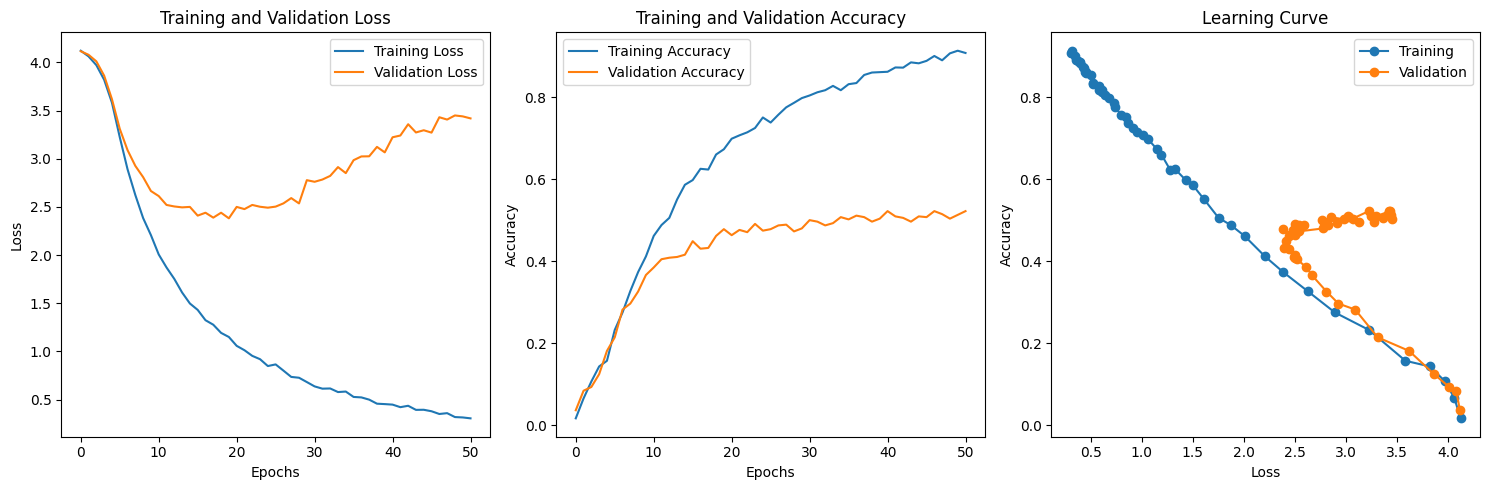
\includegraphics[width=469.5pt,height=154.3993pt]{latexImage_fc27cf5ada5744081f5d6faec9cd3059.png}}
\put(84,-360.4501){\fontsize{9.75}{1}\usefont{T1}{cmr}{m}{n}\selectfont\color{color_29791}MLP Test Accuracy: 0.5337}
\put(84,-373.2001){\fontsize{9.75}{1}\usefont{T1}{cmr}{m}{n}\selectfont\color{color_29791}MLP Test Precision: 0.5622}
\put(84,-385.9502){\fontsize{9.75}{1}\usefont{T1}{cmr}{m}{n}\selectfont\color{color_29791}MLP Test Recall: 0.5337}
\put(84,-398.7003){\fontsize{9.75}{1}\usefont{T1}{cmr}{m}{n}\selectfont\color{color_29791}MLP Test F1-Score: 0.5372}
\put(84,-424.2004){\fontsize{9.75}{1}\usefont{T1}{cmr}{m}{n}\selectfont\color{color_29791}=== Model Comparison ===}
\put(84,-436.9505){\fontsize{9.75}{1}\usefont{T1}{cmr}{m}{n}\selectfont\color{color_29791}PLA Test Accuracy: 0.2419}
\put(84,-449.7006){\fontsize{9.75}{1}\usefont{T1}{cmr}{m}{n}\selectfont\color{color_29791}MLP Test Accuracy: 0.5337}
\put(84,-462.4507){\fontsize{9.75}{1}\usefont{T1}{cmr}{m}{n}\selectfont\color{color_29791}Improvement: 29.18\%}
\put(80.25,-658.2165){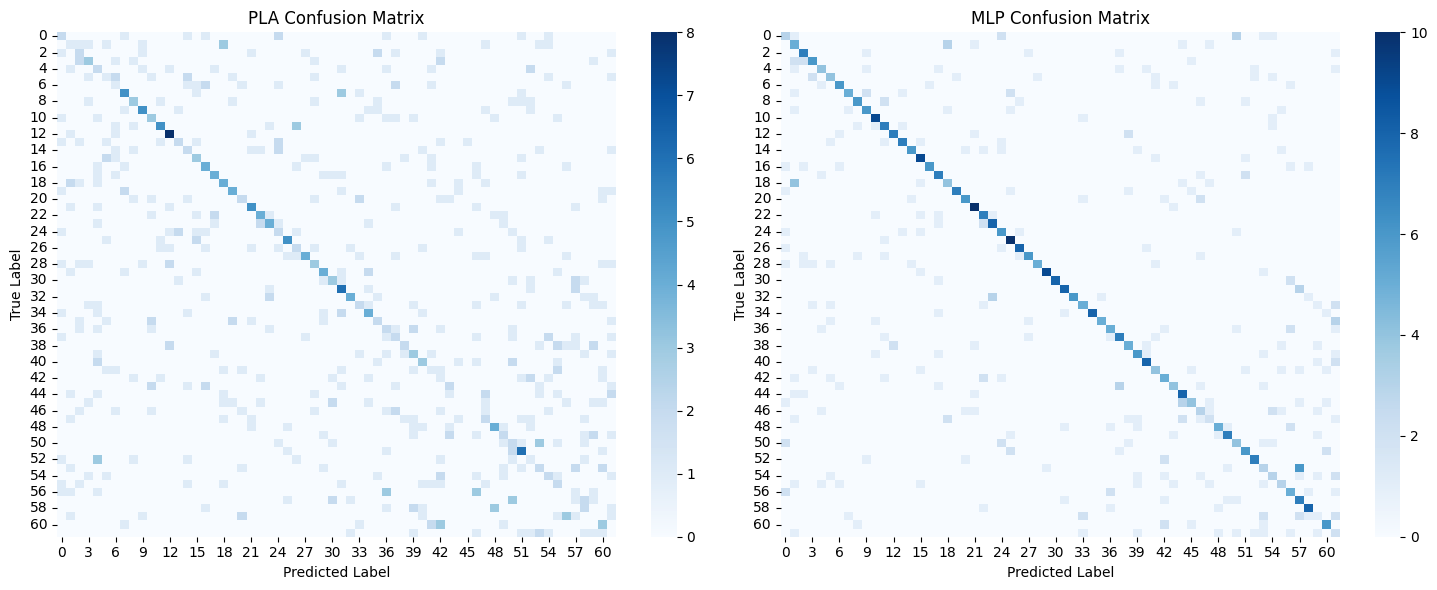
\includegraphics[width=469.5pt,height=192.7662pt]{latexImage_e183ad547ec7fa1e9d60d06d8848fe20.png}}
\end{picture}
\newpage
\begin{tikzpicture}[overlay]
\path(0pt,0pt);
\filldraw[color_283006][even odd rule]
(21pt, -746pt) -- (561pt, -746pt)
 -- (561pt, -746pt)
 -- (561pt, -26pt)
 -- (561pt, -26pt)
 -- (21pt, -26pt) -- cycle
;
\begin{scope}
\clip
(32.25pt, -236.7856pt) -- (549.75pt, -236.7856pt)
 -- (549.75pt, -236.7856pt)
 -- (549.75pt, -41pt)
 -- (549.75pt, -41pt)
 -- (32.25pt, -41pt) -- cycle
;
\end{scope}
\end{tikzpicture}
\begin{picture}(-5,0)(2.5,0)
\put(80.25,-234.4861){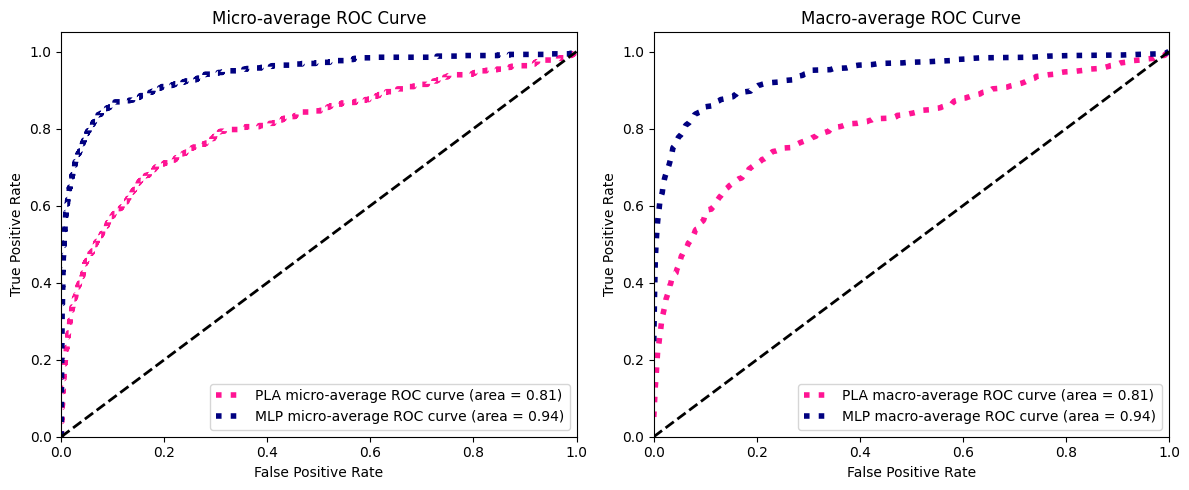
\includegraphics[width=469.5pt,height=193.4861pt]{latexImage_c35c5364bab472d5e1f45197e4a3bd9c.png}}
\end{picture}
\newpage
\begin{tikzpicture}[overlay]
\path(0pt,0pt);
\filldraw[color_283006][even odd rule]
(21pt, -746pt) -- (561pt, -746pt)
 -- (561pt, -746pt)
 -- (561pt, -26pt)
 -- (561pt, -26pt)
 -- (21pt, -26pt) -- cycle
;
\begin{scope}
\clip
(32.25pt, -729.5041pt) -- (549.75pt, -729.5041pt)
 -- (549.75pt, -729.5041pt)
 -- (549.75pt, -41pt)
 -- (549.75pt, -41pt)
 -- (32.25pt, -41pt) -- cycle
;
\end{scope}
\end{tikzpicture}
\begin{picture}(-5,0)(2.5,0)
\put(84,-50.75043){\fontsize{9.75}{1}\usefont{T1}{cmr}{m}{n}\selectfont\color{color_29791}Classification Report for PLA:}
\put(166.1799,-63.50049){\fontsize{9.75}{1}\usefont{T1}{cmr}{m}{n}\selectfont\color{color_29791}precision    recall  f1-score   support}
\put(148.5699,-89.00061){\fontsize{9.75}{1}\usefont{T1}{cmr}{m}{n}\selectfont\color{color_29791}0       0.15      0.18      0.17        11}
\put(148.5699,-101.7507){\fontsize{9.75}{1}\usefont{T1}{cmr}{m}{n}\selectfont\color{color_29791}1       0.08      0.09      0.09        11}
\put(148.5699,-114.5008){\fontsize{9.75}{1}\usefont{T1}{cmr}{m}{n}\selectfont\color{color_29791}2       0.17      0.18      0.17        11}
\put(148.5699,-127.2509){\fontsize{9.75}{1}\usefont{T1}{cmr}{m}{n}\selectfont\color{color_29791}3       0.30      0.27      0.29        11}
\put(148.5699,-140.0009){\fontsize{9.75}{1}\usefont{T1}{cmr}{m}{n}\selectfont\color{color_29791}4       0.11      0.18      0.13        11}
\put(148.5699,-152.751){\fontsize{9.75}{1}\usefont{T1}{cmr}{m}{n}\selectfont\color{color_29791}5       0.11      0.09      0.10        11}
\put(148.5699,-165.5011){\fontsize{9.75}{1}\usefont{T1}{cmr}{m}{n}\selectfont\color{color_29791}6       0.09      0.09      0.09        11}
\put(148.5699,-178.2512){\fontsize{9.75}{1}\usefont{T1}{cmr}{m}{n}\selectfont\color{color_29791}7       0.42      0.45      0.43        11}
\put(148.5699,-191.0012){\fontsize{9.75}{1}\usefont{T1}{cmr}{m}{n}\selectfont\color{color_29791}8       0.33      0.27      0.30        11}
\put(148.5699,-203.7513){\fontsize{9.75}{1}\usefont{T1}{cmr}{m}{n}\selectfont\color{color_29791}9       0.50      0.45      0.48        11}
\put(148.5699,-216.5014){\fontsize{9.75}{1}\usefont{T1}{cmr}{m}{n}\selectfont\color{color_29791}A       0.25      0.27      0.26        11}
\put(148.5699,-229.2515){\fontsize{9.75}{1}\usefont{T1}{cmr}{m}{n}\selectfont\color{color_29791}B       0.50      0.45      0.48        11}
\put(148.5699,-242.0015){\fontsize{9.75}{1}\usefont{T1}{cmr}{m}{n}\selectfont\color{color_29791}C       0.50      0.73      0.59        11}
\put(148.5699,-254.7516){\fontsize{9.75}{1}\usefont{T1}{cmr}{m}{n}\selectfont\color{color_29791}D       0.33      0.18      0.24        11}
\put(148.5699,-267.5017){\fontsize{9.75}{1}\usefont{T1}{cmr}{m}{n}\selectfont\color{color_29791}E       0.18      0.18      0.18        11}
\put(148.5699,-280.2518){\fontsize{9.75}{1}\usefont{T1}{cmr}{m}{n}\selectfont\color{color_29791}F       0.27      0.27      0.27        11}
\put(148.5699,-293.0018){\fontsize{9.75}{1}\usefont{T1}{cmr}{m}{n}\selectfont\color{color_29791}G       0.31      0.36      0.33        11}
\put(148.5699,-305.7519){\fontsize{9.75}{1}\usefont{T1}{cmr}{m}{n}\selectfont\color{color_29791}H       0.44      0.36      0.40        11}
\put(148.5699,-318.502){\fontsize{9.75}{1}\usefont{T1}{cmr}{m}{n}\selectfont\color{color_29791}I       0.33      0.36      0.35        11}
\put(148.5699,-331.2521){\fontsize{9.75}{1}\usefont{T1}{cmr}{m}{n}\selectfont\color{color_29791}J       0.44      0.36      0.40        11}
\put(148.5699,-344.0021){\fontsize{9.75}{1}\usefont{T1}{cmr}{m}{n}\selectfont\color{color_29791}K       0.25      0.18      0.21        11}
\put(148.5699,-356.7522){\fontsize{9.75}{1}\usefont{T1}{cmr}{m}{n}\selectfont\color{color_29791}L       0.42      0.45      0.43        11}
\put(148.5699,-369.5023){\fontsize{9.75}{1}\usefont{T1}{cmr}{m}{n}\selectfont\color{color_29791}M       0.44      0.36      0.40        11}
\put(148.5699,-382.2524){\fontsize{9.75}{1}\usefont{T1}{cmr}{m}{n}\selectfont\color{color_29791}N       0.40      0.36      0.38        11}
\put(148.5699,-395.0024){\fontsize{9.75}{1}\usefont{T1}{cmr}{m}{n}\selectfont\color{color_29791}O       0.17      0.18      0.17        11}
\put(148.5699,-407.7525){\fontsize{9.75}{1}\usefont{T1}{cmr}{m}{n}\selectfont\color{color_29791}P       0.56      0.45      0.50        11}
\put(148.5699,-420.5026){\fontsize{9.75}{1}\usefont{T1}{cmr}{m}{n}\selectfont\color{color_29791}Q       0.22      0.18      0.20        11}
\put(148.5699,-433.2527){\fontsize{9.75}{1}\usefont{T1}{cmr}{m}{n}\selectfont\color{color_29791}R       0.57      0.36      0.44        11}
\put(148.5699,-446.0027){\fontsize{9.75}{1}\usefont{T1}{cmr}{m}{n}\selectfont\color{color_29791}S       0.27      0.27      0.27        11}
\put(148.5699,-458.7528){\fontsize{9.75}{1}\usefont{T1}{cmr}{m}{n}\selectfont\color{color_29791}T       0.40      0.36      0.38        11}
\put(148.5699,-471.5029){\fontsize{9.75}{1}\usefont{T1}{cmr}{m}{n}\selectfont\color{color_29791}U       0.30      0.27      0.29        11}
\put(148.5699,-484.253){\fontsize{9.75}{1}\usefont{T1}{cmr}{m}{n}\selectfont\color{color_29791}V       0.32      0.55      0.40        11}
\put(148.5699,-497.003){\fontsize{9.75}{1}\usefont{T1}{cmr}{m}{n}\selectfont\color{color_29791}W       0.57      0.36      0.44        11}
\put(148.5699,-509.7531){\fontsize{9.75}{1}\usefont{T1}{cmr}{m}{n}\selectfont\color{color_29791}X       0.22      0.18      0.20        11}
\put(148.5699,-522.5032){\fontsize{9.75}{1}\usefont{T1}{cmr}{m}{n}\selectfont\color{color_29791}Y       0.33      0.36      0.35        11}
\put(148.5699,-535.2533){\fontsize{9.75}{1}\usefont{T1}{cmr}{m}{n}\selectfont\color{color_29791}Z       0.22      0.18      0.20        11}
\put(148.5699,-548.0033){\fontsize{9.75}{1}\usefont{T1}{cmr}{m}{n}\selectfont\color{color_29791}a       0.14      0.18      0.16        11}
\put(148.5699,-560.7534){\fontsize{9.75}{1}\usefont{T1}{cmr}{m}{n}\selectfont\color{color_29791}b       0.17      0.18      0.17        11}
\put(148.5699,-573.5035){\fontsize{9.75}{1}\usefont{T1}{cmr}{m}{n}\selectfont\color{color_29791}c       0.40      0.18      0.25        11}
\put(148.5699,-586.2536){\fontsize{9.75}{1}\usefont{T1}{cmr}{m}{n}\selectfont\color{color_29791}d       0.21      0.27      0.24        11}
\put(148.5699,-599.0036){\fontsize{9.75}{1}\usefont{T1}{cmr}{m}{n}\selectfont\color{color_29791}e       0.27      0.27      0.27        11}
\put(148.5699,-611.7537){\fontsize{9.75}{1}\usefont{T1}{cmr}{m}{n}\selectfont\color{color_29791}f       0.10      0.09      0.10        11}
\put(148.5699,-624.5038){\fontsize{9.75}{1}\usefont{T1}{cmr}{m}{n}\selectfont\color{color_29791}g       0.06      0.09      0.07        11}
\put(148.5699,-637.2539){\fontsize{9.75}{1}\usefont{T1}{cmr}{m}{n}\selectfont\color{color_29791}h       0.29      0.18      0.22        11}
\put(148.5699,-650.0039){\fontsize{9.75}{1}\usefont{T1}{cmr}{m}{n}\selectfont\color{color_29791}i       0.00      0.00      0.00        11}
\put(148.5699,-662.754){\fontsize{9.75}{1}\usefont{T1}{cmr}{m}{n}\selectfont\color{color_29791}j       0.00      0.00      0.00        11}
\put(148.5699,-675.5041){\fontsize{9.75}{1}\usefont{T1}{cmr}{m}{n}\selectfont\color{color_29791}k       0.00      0.00      0.00        11}
\put(148.5699,-688.2542){\fontsize{9.75}{1}\usefont{T1}{cmr}{m}{n}\selectfont\color{color_29791}l       0.18      0.18      0.18        11}
\put(148.5699,-701.0042){\fontsize{9.75}{1}\usefont{T1}{cmr}{m}{n}\selectfont\color{color_29791}m       0.40      0.36      0.38        11}
\put(148.5699,-713.7543){\fontsize{9.75}{1}\usefont{T1}{cmr}{m}{n}\selectfont\color{color_29791}n       0.22      0.18      0.20        11}
\put(148.5699,-726.5044){\fontsize{9.75}{1}\usefont{T1}{cmr}{m}{n}\selectfont\color{color_29791}o       0.13      0.18      0.15        11}
\end{picture}
\newpage
\begin{tikzpicture}[overlay]
\path(0pt,0pt);
\filldraw[color_283006][even odd rule]
(21pt, -746pt) -- (561pt, -746pt)
 -- (561pt, -746pt)
 -- (561pt, -26pt)
 -- (561pt, -26pt)
 -- (21pt, -26pt) -- cycle
;
\begin{scope}
\clip
(32.25pt, -729.5041pt) -- (549.75pt, -729.5041pt)
 -- (549.75pt, -729.5041pt)
 -- (549.75pt, -41pt)
 -- (549.75pt, -41pt)
 -- (32.25pt, -41pt) -- cycle
;
\end{scope}
\end{tikzpicture}
\begin{picture}(-5,0)(2.5,0)
\put(148.5699,-50.75043){\fontsize{9.75}{1}\usefont{T1}{cmr}{m}{n}\selectfont\color{color_29791}p       0.32      0.55      0.40        11}
\put(148.5699,-63.50049){\fontsize{9.75}{1}\usefont{T1}{cmr}{m}{n}\selectfont\color{color_29791}q       0.08      0.09      0.09        11}
\put(148.5699,-76.25061){\fontsize{9.75}{1}\usefont{T1}{cmr}{m}{n}\selectfont\color{color_29791}r       0.17      0.18      0.17        11}
\put(148.5699,-89.00061){\fontsize{9.75}{1}\usefont{T1}{cmr}{m}{n}\selectfont\color{color_29791}s       0.18      0.18      0.18        11}
\put(148.5699,-101.7507){\fontsize{9.75}{1}\usefont{T1}{cmr}{m}{n}\selectfont\color{color_29791}t       0.15      0.18      0.17        11}
\put(148.5699,-114.5008){\fontsize{9.75}{1}\usefont{T1}{cmr}{m}{n}\selectfont\color{color_29791}u       0.00      0.00      0.00        11}
\put(148.5699,-127.2509){\fontsize{9.75}{1}\usefont{T1}{cmr}{m}{n}\selectfont\color{color_29791}v       0.08      0.09      0.09        11}
\put(148.5699,-140.0009){\fontsize{9.75}{1}\usefont{T1}{cmr}{m}{n}\selectfont\color{color_29791}w       0.17      0.18      0.17        11}
\put(148.5699,-152.751){\fontsize{9.75}{1}\usefont{T1}{cmr}{m}{n}\selectfont\color{color_29791}x       0.00      0.00      0.00        11}
\put(148.5699,-165.5011){\fontsize{9.75}{1}\usefont{T1}{cmr}{m}{n}\selectfont\color{color_29791}y       0.21      0.27      0.24        11}
\put(148.5699,-178.2512){\fontsize{9.75}{1}\usefont{T1}{cmr}{m}{n}\selectfont\color{color_29791}z       0.00      0.00      0.00        11}
\put(107.48,-203.7513){\fontsize{9.75}{1}\usefont{T1}{cmr}{m}{n}\selectfont\color{color_29791}accuracy                           0.24       682}
\put(101.61,-216.5014){\fontsize{9.75}{1}\usefont{T1}{cmr}{m}{n}\selectfont\color{color_29791}macro avg       0.25      0.24      0.24       682}
\put(84,-229.2515){\fontsize{9.75}{1}\usefont{T1}{cmr}{m}{n}\selectfont\color{color_29791}weighted avg       0.25      0.24      0.24       682}
\put(84,-267.5017){\fontsize{9.75}{1}\usefont{T1}{cmr}{m}{n}\selectfont\color{color_29791}Classification Report for MLP:}
\put(166.1799,-280.2518){\fontsize{9.75}{1}\usefont{T1}{cmr}{m}{n}\selectfont\color{color_29791}precision    recall  f1-score   support}
\put(148.5699,-305.7519){\fontsize{9.75}{1}\usefont{T1}{cmr}{m}{n}\selectfont\color{color_29791}0       0.23      0.27      0.25        11}
\put(148.5699,-318.502){\fontsize{9.75}{1}\usefont{T1}{cmr}{m}{n}\selectfont\color{color_29791}1       0.25      0.45      0.32        11}
\put(148.5699,-331.2521){\fontsize{9.75}{1}\usefont{T1}{cmr}{m}{n}\selectfont\color{color_29791}2       0.54      0.64      0.58        11}
\put(148.5699,-344.0021){\fontsize{9.75}{1}\usefont{T1}{cmr}{m}{n}\selectfont\color{color_29791}3       0.55      0.55      0.55        11}
\put(148.5699,-356.7522){\fontsize{9.75}{1}\usefont{T1}{cmr}{m}{n}\selectfont\color{color_29791}4       0.44      0.36      0.40        11}
\put(148.5699,-369.5023){\fontsize{9.75}{1}\usefont{T1}{cmr}{m}{n}\selectfont\color{color_29791}5       0.40      0.36      0.38        11}
\put(148.5699,-382.2524){\fontsize{9.75}{1}\usefont{T1}{cmr}{m}{n}\selectfont\color{color_29791}6       0.60      0.55      0.57        11}
\put(148.5699,-395.0024){\fontsize{9.75}{1}\usefont{T1}{cmr}{m}{n}\selectfont\color{color_29791}7       0.71      0.45      0.56        11}
\put(148.5699,-407.7525){\fontsize{9.75}{1}\usefont{T1}{cmr}{m}{n}\selectfont\color{color_29791}8       0.67      0.55      0.60        11}
\put(148.5699,-420.5026){\fontsize{9.75}{1}\usefont{T1}{cmr}{m}{n}\selectfont\color{color_29791}9       0.55      0.55      0.55        11}
\put(148.5699,-433.2527){\fontsize{9.75}{1}\usefont{T1}{cmr}{m}{n}\selectfont\color{color_29791}A       0.69      0.82      0.75        11}
\put(148.5699,-446.0027){\fontsize{9.75}{1}\usefont{T1}{cmr}{m}{n}\selectfont\color{color_29791}B       0.50      0.64      0.56        11}
\put(148.5699,-458.7528){\fontsize{9.75}{1}\usefont{T1}{cmr}{m}{n}\selectfont\color{color_29791}C       0.78      0.64      0.70        11}
\put(148.5699,-471.5029){\fontsize{9.75}{1}\usefont{T1}{cmr}{m}{n}\selectfont\color{color_29791}D       0.70      0.64      0.67        11}
\put(148.5699,-484.253){\fontsize{9.75}{1}\usefont{T1}{cmr}{m}{n}\selectfont\color{color_29791}E       0.75      0.55      0.63        11}
\put(148.5699,-497.003){\fontsize{9.75}{1}\usefont{T1}{cmr}{m}{n}\selectfont\color{color_29791}F       0.56      0.82      0.67        11}
\put(148.5699,-509.7531){\fontsize{9.75}{1}\usefont{T1}{cmr}{m}{n}\selectfont\color{color_29791}G       0.86      0.55      0.67        11}
\put(148.5699,-522.5032){\fontsize{9.75}{1}\usefont{T1}{cmr}{m}{n}\selectfont\color{color_29791}H       0.50      0.64      0.56        11}
\put(148.5699,-535.2533){\fontsize{9.75}{1}\usefont{T1}{cmr}{m}{n}\selectfont\color{color_29791}I       0.40      0.36      0.38        11}
\put(148.5699,-548.0033){\fontsize{9.75}{1}\usefont{T1}{cmr}{m}{n}\selectfont\color{color_29791}J       0.88      0.64      0.74        11}
\put(148.5699,-560.7534){\fontsize{9.75}{1}\usefont{T1}{cmr}{m}{n}\selectfont\color{color_29791}K       0.67      0.55      0.60        11}
\put(148.5699,-573.5035){\fontsize{9.75}{1}\usefont{T1}{cmr}{m}{n}\selectfont\color{color_29791}L       0.67      0.91      0.77        11}
\put(148.5699,-586.2536){\fontsize{9.75}{1}\usefont{T1}{cmr}{m}{n}\selectfont\color{color_29791}M       0.50      0.64      0.56        11}
\put(148.5699,-599.0036){\fontsize{9.75}{1}\usefont{T1}{cmr}{m}{n}\selectfont\color{color_29791}N       0.67      0.73      0.70        11}
\put(148.5699,-611.7537){\fontsize{9.75}{1}\usefont{T1}{cmr}{m}{n}\selectfont\color{color_29791}O       0.43      0.55      0.48        11}
\put(148.5699,-624.5038){\fontsize{9.75}{1}\usefont{T1}{cmr}{m}{n}\selectfont\color{color_29791}P       0.59      0.91      0.71        11}
\put(148.5699,-637.2539){\fontsize{9.75}{1}\usefont{T1}{cmr}{m}{n}\selectfont\color{color_29791}Q       0.73      0.73      0.73        11}
\put(148.5699,-650.0039){\fontsize{9.75}{1}\usefont{T1}{cmr}{m}{n}\selectfont\color{color_29791}R       0.67      0.55      0.60        11}
\put(148.5699,-662.754){\fontsize{9.75}{1}\usefont{T1}{cmr}{m}{n}\selectfont\color{color_29791}S       0.83      0.45      0.59        11}
\put(148.5699,-675.5041){\fontsize{9.75}{1}\usefont{T1}{cmr}{m}{n}\selectfont\color{color_29791}T       0.90      0.82      0.86        11}
\put(148.5699,-688.2542){\fontsize{9.75}{1}\usefont{T1}{cmr}{m}{n}\selectfont\color{color_29791}U       1.00      0.73      0.84        11}
\put(148.5699,-701.0042){\fontsize{9.75}{1}\usefont{T1}{cmr}{m}{n}\selectfont\color{color_29791}V       0.73      0.73      0.73        11}
\put(148.5699,-713.7543){\fontsize{9.75}{1}\usefont{T1}{cmr}{m}{n}\selectfont\color{color_29791}W       1.00      0.55      0.71        11}
\put(148.5699,-726.5044){\fontsize{9.75}{1}\usefont{T1}{cmr}{m}{n}\selectfont\color{color_29791}X       0.50      0.45      0.48        11}
\end{picture}
\newpage
\begin{tikzpicture}[overlay]
\path(0pt,0pt);
\filldraw[color_283006][even odd rule]
(21pt, -746pt) -- (561pt, -746pt)
 -- (561pt, -746pt)
 -- (561pt, -26pt)
 -- (561pt, -26pt)
 -- (21pt, -26pt) -- cycle
;
\begin{scope}
\clip
(32.25pt, -461.7525pt) -- (549.75pt, -461.7525pt)
 -- (549.75pt, -461.7525pt)
 -- (549.75pt, -41pt)
 -- (549.75pt, -41pt)
 -- (32.25pt, -41pt) -- cycle
;
\end{scope}
\end{tikzpicture}
\begin{picture}(-5,0)(2.5,0)
\put(148.5699,-50.75043){\fontsize{9.75}{1}\usefont{T1}{cmr}{m}{n}\selectfont\color{color_29791}Y       1.00      0.73      0.84        11}
\put(148.5699,-63.50049){\fontsize{9.75}{1}\usefont{T1}{cmr}{m}{n}\selectfont\color{color_29791}Z       0.83      0.45      0.59        11}
\put(148.5699,-76.25061){\fontsize{9.75}{1}\usefont{T1}{cmr}{m}{n}\selectfont\color{color_29791}a       0.50      0.45      0.48        11}
\put(148.5699,-89.00061){\fontsize{9.75}{1}\usefont{T1}{cmr}{m}{n}\selectfont\color{color_29791}b       0.54      0.64      0.58        11}
\put(148.5699,-101.7507){\fontsize{9.75}{1}\usefont{T1}{cmr}{m}{n}\selectfont\color{color_29791}c       0.50      0.45      0.48        11}
\put(148.5699,-114.5008){\fontsize{9.75}{1}\usefont{T1}{cmr}{m}{n}\selectfont\color{color_29791}d       0.50      0.55      0.52        11}
\put(148.5699,-127.2509){\fontsize{9.75}{1}\usefont{T1}{cmr}{m}{n}\selectfont\color{color_29791}e       0.67      0.73      0.70        11}
\put(148.5699,-140.0009){\fontsize{9.75}{1}\usefont{T1}{cmr}{m}{n}\selectfont\color{color_29791}f       0.44      0.36      0.40        11}
\put(148.5699,-152.751){\fontsize{9.75}{1}\usefont{T1}{cmr}{m}{n}\selectfont\color{color_29791}g       0.38      0.45      0.42        11}
\put(148.5699,-165.5011){\fontsize{9.75}{1}\usefont{T1}{cmr}{m}{n}\selectfont\color{color_29791}h       0.50      0.36      0.42        11}
\put(148.5699,-178.2512){\fontsize{9.75}{1}\usefont{T1}{cmr}{m}{n}\selectfont\color{color_29791}i       0.53      0.73      0.62        11}
\put(148.5699,-191.0012){\fontsize{9.75}{1}\usefont{T1}{cmr}{m}{n}\selectfont\color{color_29791}j       0.50      0.36      0.42        11}
\put(148.5699,-203.7513){\fontsize{9.75}{1}\usefont{T1}{cmr}{m}{n}\selectfont\color{color_29791}k       0.27      0.27      0.27        11}
\put(148.5699,-216.5014){\fontsize{9.75}{1}\usefont{T1}{cmr}{m}{n}\selectfont\color{color_29791}l       0.29      0.18      0.22        11}
\put(148.5699,-229.2515){\fontsize{9.75}{1}\usefont{T1}{cmr}{m}{n}\selectfont\color{color_29791}m       0.62      0.45      0.53        11}
\put(148.5699,-242.0015){\fontsize{9.75}{1}\usefont{T1}{cmr}{m}{n}\selectfont\color{color_29791}n       0.70      0.64      0.67        11}
\put(148.5699,-254.7516){\fontsize{9.75}{1}\usefont{T1}{cmr}{m}{n}\selectfont\color{color_29791}o       0.36      0.36      0.36        11}
\put(148.5699,-267.5017){\fontsize{9.75}{1}\usefont{T1}{cmr}{m}{n}\selectfont\color{color_29791}p       0.55      0.55      0.55        11}
\put(148.5699,-280.2518){\fontsize{9.75}{1}\usefont{T1}{cmr}{m}{n}\selectfont\color{color_29791}q       0.70      0.64      0.67        11}
\put(148.5699,-293.0018){\fontsize{9.75}{1}\usefont{T1}{cmr}{m}{n}\selectfont\color{color_29791}r       0.23      0.27      0.25        11}
\put(148.5699,-305.7519){\fontsize{9.75}{1}\usefont{T1}{cmr}{m}{n}\selectfont\color{color_29791}s       0.30      0.27      0.29        11}
\put(148.5699,-318.502){\fontsize{9.75}{1}\usefont{T1}{cmr}{m}{n}\selectfont\color{color_29791}t       0.38      0.27      0.32        11}
\put(148.5699,-331.2521){\fontsize{9.75}{1}\usefont{T1}{cmr}{m}{n}\selectfont\color{color_29791}u       0.36      0.45      0.40        11}
\put(148.5699,-344.0021){\fontsize{9.75}{1}\usefont{T1}{cmr}{m}{n}\selectfont\color{color_29791}v       0.33      0.64      0.44        11}
\put(148.5699,-356.7522){\fontsize{9.75}{1}\usefont{T1}{cmr}{m}{n}\selectfont\color{color_29791}w       0.67      0.73      0.70        11}
\put(148.5699,-369.5023){\fontsize{9.75}{1}\usefont{T1}{cmr}{m}{n}\selectfont\color{color_29791}x       0.12      0.09      0.11        11}
\put(148.5699,-382.2524){\fontsize{9.75}{1}\usefont{T1}{cmr}{m}{n}\selectfont\color{color_29791}y       0.55      0.55      0.55        11}
\put(148.5699,-395.0024){\fontsize{9.75}{1}\usefont{T1}{cmr}{m}{n}\selectfont\color{color_29791}z       0.11      0.18      0.13        11}
\put(107.48,-420.5026){\fontsize{9.75}{1}\usefont{T1}{cmr}{m}{n}\selectfont\color{color_29791}accuracy                           0.53       682}
\put(101.61,-433.2527){\fontsize{9.75}{1}\usefont{T1}{cmr}{m}{n}\selectfont\color{color_29791}macro avg       0.56      0.53      0.54       682}
\put(84,-446.0027){\fontsize{9.75}{1}\usefont{T1}{cmr}{m}{n}\selectfont\color{color_29791}weighted avg       0.56      0.53      0.54       682}
\put(80.25,-654.2183){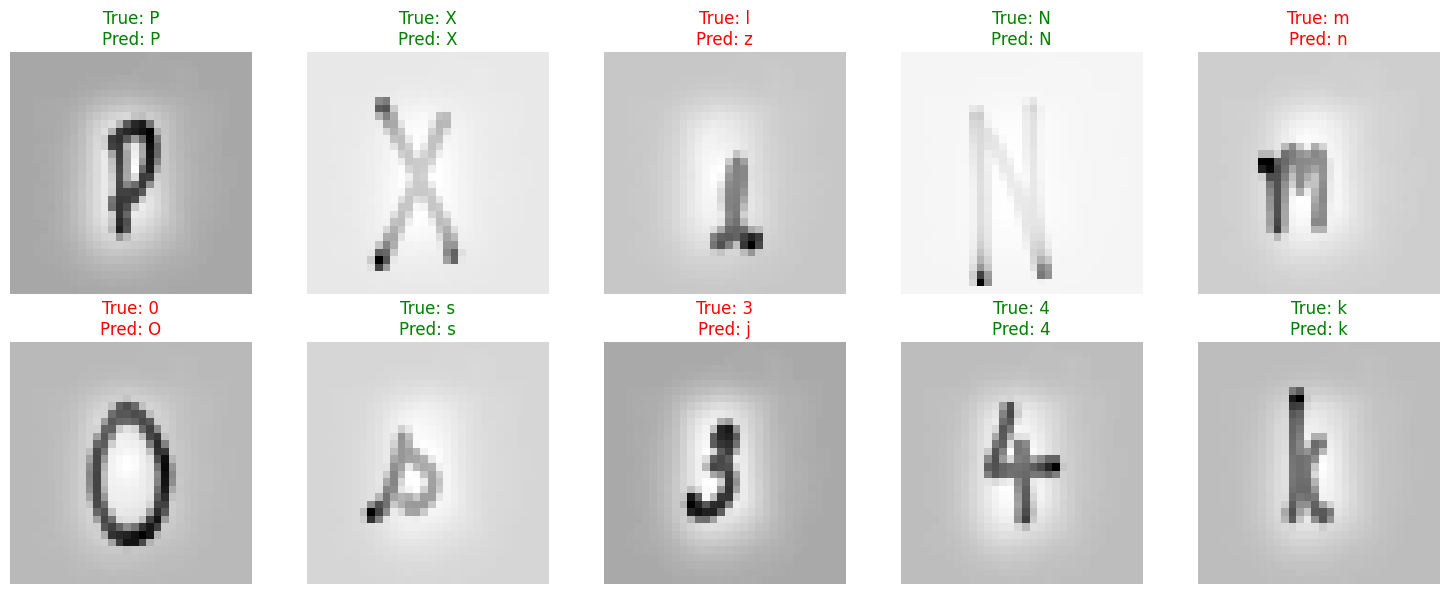
\includegraphics[width=469.5pt,height=192.4658pt]{latexImage_1a172c0fefe6c87e218d46a16f6542b5.png}}
\end{picture}
\newpage
\begin{tikzpicture}[overlay]
\path(0pt,0pt);
\filldraw[color_283006][even odd rule]
(21pt, -746pt) -- (561pt, -746pt)
 -- (561pt, -746pt)
 -- (561pt, -26pt)
 -- (561pt, -26pt)
 -- (21pt, -26pt) -- cycle
;
\begin{scope}
\clip
(32.25pt, -222.4006pt) -- (549.75pt, -222.4006pt)
 -- (549.75pt, -222.4006pt)
 -- (549.75pt, -37.25pt)
 -- (549.75pt, -37.25pt)
 -- (32.25pt, -37.25pt) -- cycle
;
\filldraw[color_283006][even odd rule]
(195.154pt, -154.2267pt) -- (255.3774pt, -154.2267pt)
 -- (255.3774pt, -154.2267pt)
 -- (255.3774pt, -132.3771pt)
 -- (255.3774pt, -132.3771pt)
 -- (195.154pt, -132.3771pt) -- cycle
;
\filldraw[color_283006][even odd rule]
(255.3774pt, -154.2267pt) -- (302.304pt, -154.2267pt)
 -- (302.304pt, -154.2267pt)
 -- (302.304pt, -132.3771pt)
 -- (302.304pt, -132.3771pt)
 -- (255.3774pt, -132.3771pt) -- cycle
;
\filldraw[color_283006][even odd rule]
(302.304pt, -154.2267pt) -- (349.2306pt, -154.2267pt)
 -- (349.2306pt, -154.2267pt)
 -- (349.2306pt, -132.3771pt)
 -- (349.2306pt, -132.3771pt)
 -- (302.304pt, -132.3771pt) -- cycle
;
\filldraw[color_283006][even odd rule]
(349.2307pt, -154.2267pt) -- (432.5961pt, -154.2267pt)
 -- (432.5961pt, -154.2267pt)
 -- (432.5961pt, -132.3771pt)
 -- (432.5961pt, -132.3771pt)
 -- (349.2307pt, -132.3771pt) -- cycle
;
\filldraw[color_273076][even odd rule]
(195.154pt, -175.3263pt) -- (255.3774pt, -175.3263pt)
 -- (255.3774pt, -175.3263pt)
 -- (255.3774pt, -154.2267pt)
 -- (255.3774pt, -154.2267pt)
 -- (195.154pt, -154.2267pt) -- cycle
;
\filldraw[color_273076][even odd rule]
(255.3774pt, -175.3263pt) -- (302.304pt, -175.3263pt)
 -- (302.304pt, -175.3263pt)
 -- (302.304pt, -154.2267pt)
 -- (302.304pt, -154.2267pt)
 -- (255.3774pt, -154.2267pt) -- cycle
;
\filldraw[color_273076][even odd rule]
(302.304pt, -175.3263pt) -- (349.2306pt, -175.3263pt)
 -- (349.2306pt, -175.3263pt)
 -- (349.2306pt, -154.2267pt)
 -- (349.2306pt, -154.2267pt)
 -- (302.304pt, -154.2267pt) -- cycle
;
\filldraw[color_273076][even odd rule]
(349.2307pt, -175.3263pt) -- (432.5961pt, -175.3263pt)
 -- (432.5961pt, -175.3263pt)
 -- (432.5961pt, -154.2267pt)
 -- (432.5961pt, -154.2267pt)
 -- (349.2307pt, -154.2267pt) -- cycle
;
\filldraw[color_283006][even odd rule]
(195.154pt, -196.426pt) -- (255.3774pt, -196.426pt)
 -- (255.3774pt, -196.426pt)
 -- (255.3774pt, -175.3264pt)
 -- (255.3774pt, -175.3264pt)
 -- (195.154pt, -175.3264pt) -- cycle
;
\filldraw[color_283006][even odd rule]
(255.3774pt, -196.426pt) -- (302.304pt, -196.426pt)
 -- (302.304pt, -196.426pt)
 -- (302.304pt, -175.3264pt)
 -- (302.304pt, -175.3264pt)
 -- (255.3774pt, -175.3264pt) -- cycle
;
\filldraw[color_283006][even odd rule]
(302.304pt, -196.426pt) -- (349.2306pt, -196.426pt)
 -- (349.2306pt, -196.426pt)
 -- (349.2306pt, -175.3264pt)
 -- (349.2306pt, -175.3264pt)
 -- (302.304pt, -175.3264pt) -- cycle
;
\filldraw[color_283006][even odd rule]
(349.2307pt, -196.426pt) -- (432.5961pt, -196.426pt)
 -- (432.5961pt, -196.426pt)
 -- (432.5961pt, -175.3264pt)
 -- (432.5961pt, -175.3264pt)
 -- (349.2307pt, -175.3264pt) -- cycle
;
\filldraw[color_273076][even odd rule]
(195.154pt, -217.5256pt) -- (255.3774pt, -217.5256pt)
 -- (255.3774pt, -217.5256pt)
 -- (255.3774pt, -196.426pt)
 -- (255.3774pt, -196.426pt)
 -- (195.154pt, -196.426pt) -- cycle
;
\filldraw[color_273076][even odd rule]
(255.3774pt, -217.5256pt) -- (302.304pt, -217.5256pt)
 -- (302.304pt, -217.5256pt)
 -- (302.304pt, -196.426pt)
 -- (302.304pt, -196.426pt)
 -- (255.3774pt, -196.426pt) -- cycle
;
\filldraw[color_273076][even odd rule]
(302.304pt, -217.5256pt) -- (349.2306pt, -217.5256pt)
 -- (349.2306pt, -217.5256pt)
 -- (349.2306pt, -196.426pt)
 -- (349.2306pt, -196.426pt)
 -- (302.304pt, -196.426pt) -- cycle
;
\filldraw[color_273076][even odd rule]
(349.2307pt, -217.5256pt) -- (432.5961pt, -217.5256pt)
 -- (432.5961pt, -217.5256pt)
 -- (432.5961pt, -196.426pt)
 -- (432.5961pt, -196.426pt)
 -- (349.2307pt, -196.426pt) -- cycle
;
\filldraw[color_217468][nonzero rule]
(195.154pt, -133.1271pt) -- (432.596pt, -133.1271pt)
 -- (432.596pt, -133.1271pt)
 -- (432.596pt, -132.3771pt)
 -- (432.596pt, -132.3771pt)
 -- (195.154pt, -132.3771pt) -- cycle
;
\end{scope}
\filldraw[color_273076][even odd rule]
(89.25pt, -723.4034pt) -- (549.75pt, -723.4034pt)
 -- (549.75pt, -723.4034pt)
 -- (549.75pt, -229.9006pt)
 -- (549.75pt, -229.9006pt)
 -- (89.25pt, -229.9006pt) -- cycle
;
\filldraw[color_252223][nonzero rule]
(89.25pt, -723.4034pt) -- (89.25pt, -229.9006pt)
 -- (89.25pt, -229.9006pt)
 -- (549.75pt, -229.9006pt)
 -- (549.75pt, -229.9006pt)
 -- (549.75pt, -723.4034pt)
 -- (549.75pt, -723.4034pt)
 -- (549pt, -723.4034pt)
 -- (549pt, -723.4034pt)
 -- (549pt, -230.6506pt)
 -- (549pt, -230.6506pt)
 -- (90pt, -230.6506pt)
 -- (90pt, -230.6506pt)
 -- (90pt, -723.4034pt) -- cycle
;
\begin{scope}
\clip
(32.25pt, -723.4034pt) -- (549.75pt, -723.4034pt)
 -- (549.75pt, -723.4034pt)
 -- (549.75pt, -229.9006pt)
 -- (549.75pt, -229.9006pt)
 -- (32.25pt, -229.9006pt) -- cycle
;
\begin{scope}
\clip
(90pt, -722.6534pt) -- (549pt, -722.6534pt)
 -- (549pt, -722.6534pt)
 -- (549pt, -230.6506pt)
 -- (549pt, -230.6506pt)
 -- (90pt, -230.6506pt) -- cycle
;
\filldraw[color_273076][even odd rule]
(90pt, -722.6534pt) -- (549pt, -722.6534pt)
 -- (549pt, -722.6534pt)
 -- (549pt, -230.6506pt)
 -- (549pt, -230.6506pt)
 -- (90pt, -230.6506pt) -- cycle
;
\end{scope}
\end{scope}
\begin{scope}
\clip
(32.25pt, -222.4006pt) -- (549.75pt, -222.4006pt)
 -- (549.75pt, -222.4006pt)
 -- (549.75pt, -37.25pt)
 -- (549.75pt, -37.25pt)
 -- (32.25pt, -37.25pt) -- cycle
;
\end{scope}
\end{tikzpicture}
\begin{picture}(-5,0)(2.5,0)
\put(93,-68.73761){\fontsize{21.7728}{1}\usefont{T1}{cmr}{b}{n}\selectfont\color{color_29791}PLA vs MLP Performance}
\put(93,-90.51038){\fontsize{21.7728}{1}\usefont{T1}{cmr}{b}{n}\selectfont\color{color_29791}Comparison}
\put(207.8128,-125.2027){\fontsize{9.75}{1}\usefont{T1}{cmr}{b}{n}\selectfont\color{color_29791}MetricPLAMLPImprovement}
\put(200.029,-147.0523){\fontsize{9.75}{1}\usefont{T1}{cmr}{b}{n}\selectfont\color{color_29791}Accuracy24.19\%50.37\%+26.18\%}
\put(200.029,-168.1519){\fontsize{9.75}{1}\usefont{T1}{cmr}{b}{n}\selectfont\color{color_29791}Precision24.91\%49.83\%+24.92\%}
\put(200.029,-189.2515){\fontsize{9.75}{1}\usefont{T1}{cmr}{b}{n}\selectfont\color{color_29791}Recall24.19\%50.37\%+26.18\%}
\put(200.029,-210.3511){\fontsize{9.75}{1}\usefont{T1}{cmr}{b}{n}\selectfont\color{color_29791}F1-Score24.10\%49.52\%+25.42\%}
\put(93,-244.151){\fontsize{9.75}{1}\usefont{T1}{cmr}{m}{n}\selectfont\color{color_95391}\# A/B Experiment Comparison Visualization}
\put(93,-256.901){\fontsize{9.75}{1}\usefont{T1}{cmr}{m}{n}\selectfont\color{color_62560}print("="*70)}
\put(93,-269.6511){\fontsize{9.75}{1}\usefont{T1}{cmr}{m}{n}\selectfont\color{color_62560}print("A/B EXPERIMENT: PLA vs MLP PERFORMANCE COMPARISON")}
\put(93,-282.4012){\fontsize{9.75}{1}\usefont{T1}{cmr}{m}{n}\selectfont\color{color_62560}print("="*70)}
\put(93,-307.9013){\fontsize{9.75}{1}\usefont{T1}{cmr}{m}{n}\selectfont\color{color_95391}\# Display final chosen hyperparameters}
\put(93,-320.6514){\fontsize{9.75}{1}\usefont{T1}{cmr}{m}{n}\selectfont\color{color_62560}print("\n"+"="*70)}
\put(93,-333.4015){\fontsize{9.75}{1}\usefont{T1}{cmr}{m}{n}\selectfont\color{color_62560}print("FINAL CHOSEN HYPERPARAMETERS FOR MLP:")}
\put(93,-346.1516){\fontsize{9.75}{1}\usefont{T1}{cmr}{m}{n}\selectfont\color{color_62560}print("="*70)}
\put(93,-358.9016){\fontsize{9.75}{1}\usefont{T1}{cmr}{m}{n}\selectfont\color{color_62560}print(f"• Architecture:\{best\_params['hidden\_layers']\}hidden layers")}
\put(93,-371.6517){\fontsize{9.75}{1}\usefont{T1}{cmr}{m}{n}\selectfont\color{color_62560}print(f"• Activation Function:\{best\_params['activation']\}")}
\put(93,-384.4018){\fontsize{9.75}{1}\usefont{T1}{cmr}{m}{n}\selectfont\color{color_62560}print(f"• Learning Rate:\{best\_params['learning\_rate']\}")}
\put(93,-397.1519){\fontsize{9.75}{1}\usefont{T1}{cmr}{m}{n}\selectfont\color{color_62560}print(f"• Optimizer:\{best\_params['optimizer'].upper()\}")}
\put(93,-409.9019){\fontsize{9.75}{1}\usefont{T1}{cmr}{m}{n}\selectfont\color{color_62560}print(f"• Validation Accuracy:\{best\_val\_acc:.2\%\}")}
\put(93,-435.4021){\fontsize{9.75}{1}\usefont{T1}{cmr}{m}{n}\selectfont\color{color_95391}\# Display quantitative comparison}
\put(93,-448.1522){\fontsize{9.75}{1}\usefont{T1}{cmr}{m}{n}\selectfont\color{color_62560}print("\n"+"="*70)}
\put(93,-460.9022){\fontsize{9.75}{1}\usefont{T1}{cmr}{m}{n}\selectfont\color{color_62560}print("QUANTITATIVE PERFORMANCE COMPARISON:")}
\put(93,-473.6523){\fontsize{9.75}{1}\usefont{T1}{cmr}{m}{n}\selectfont\color{color_62560}print("="*70)}
\put(93,-486.4024){\fontsize{9.75}{1}\usefont{T1}{cmr}{m}{n}\selectfont\color{color_62560}print("+"+"-"*48+"+")}
\put(93,-499.1525){\fontsize{9.75}{1}\usefont{T1}{cmr}{m}{n}\selectfont\color{color_62560}print(f"|\{'Metric':<20\}|\{'PLA':<8\}|\{'MLP':<8\}|\{'Improvement':<12\}|")}
\put(93,-511.9025){\fontsize{9.75}{1}\usefont{T1}{cmr}{m}{n}\selectfont\color{color_62560}print("+"+"-"*48+"+")}
\put(93,-524.6526){\fontsize{9.75}{1}\usefont{T1}{cmr}{m}{n}\selectfont\color{color_62560}print(f"|\{'Accuracy':<20\}|\{pla\_accuracy:>7.2\%\}|\{mlp\_test\_acc:>7.2\%\}|\{f'+}
\put(93,-537.4027){\fontsize{9.75}{1}\usefont{T1}{cmr}{m}{n}\selectfont\color{color_62560}print(f"|\{'Precision':<20\}|\{pla\_precision:>7.2\%\}|\{mlp\_precision:>7.2\%\}|\{}
\put(93,-550.1528){\fontsize{9.75}{1}\usefont{T1}{cmr}{m}{n}\selectfont\color{color_62560}print(f"|\{'Recall':<20\}|\{pla\_recall:>7.2\%\}|\{mlp\_recall:>7.2\%\}|\{f'+\{(mlp\_recall}
\put(93,-562.9028){\fontsize{9.75}{1}\usefont{T1}{cmr}{m}{n}\selectfont\color{color_62560}print(f"|\{'F1-Score':<20\}|\{pla\_f1:>7.2\%\}|\{mlp\_f1:>7.2\%\}|\{f'+\{(mlp\_f1-pla\_f1}
\put(93,-575.6529){\fontsize{9.75}{1}\usefont{T1}{cmr}{m}{n}\selectfont\color{color_62560}print("+"+"-"*48+"+")}
\put(93,-601.1531){\fontsize{9.75}{1}\usefont{T1}{cmr}{m}{n}\selectfont\color{color_62560}relative\_improvement=((mlp\_test\_acc-pla\_accuracy)/pla\_accuracy)*100}
\put(93,-613.9031){\fontsize{9.75}{1}\usefont{T1}{cmr}{m}{n}\selectfont\color{color_62560}print(f"\nRELATIVE IMPROVEMENT:\{relative\_improvement:.1f\}\%")}
\put(93,-639.4033){\fontsize{9.75}{1}\usefont{T1}{cmr}{m}{n}\selectfont\color{color_95391}\# Display strengths and weaknesses}
\put(93,-652.1534){\fontsize{9.75}{1}\usefont{T1}{cmr}{m}{n}\selectfont\color{color_62560}print("\n"+"="*70)}
\put(93,-664.9034){\fontsize{9.75}{1}\usefont{T1}{cmr}{m}{n}\selectfont\color{color_62560}print("STRENGTHS AND WEAKNESSES ANALYSIS:")}
\put(93,-677.6535){\fontsize{9.75}{1}\usefont{T1}{cmr}{m}{n}\selectfont\color{color_62560}print("="*70)}
\put(93,-703.1537){\fontsize{9.75}{1}\usefont{T1}{cmr}{m}{n}\selectfont\color{color_62560}print("\nPLA STRENGTHS:")}
\put(93,-715.9037){\fontsize{9.75}{1}\usefont{T1}{cmr}{m}{n}\selectfont\color{color_62560}print("✓ Simple and fast to implement")}
\put(43.66,-244.151){\fontsize{9.75}{1}\usefont{T1}{cmr}{m}{n}\selectfont\color{color_126112}In[]:}
\end{picture}
\newpage
\begin{tikzpicture}[overlay]
\path(0pt,0pt);
\filldraw[color_283006][even odd rule]
(21pt, -746pt) -- (561pt, -746pt)
 -- (561pt, -746pt)
 -- (561pt, -26pt)
 -- (561pt, -26pt)
 -- (21pt, -26pt) -- cycle
;
\filldraw[color_273076][even odd rule]
(89.25pt, -722.004pt) -- (549.75pt, -722.004pt)
 -- (549.75pt, -722.004pt)
 -- (549.75pt, -37.25pt)
 -- (549.75pt, -37.25pt)
 -- (89.25pt, -37.25pt) -- cycle
;
\filldraw[color_252223][nonzero rule]
(89.25pt, -722.004pt) -- (90pt, -722.004pt)
 -- (90pt, -722.004pt)
 -- (90pt, -37.25pt)
 -- (90pt, -37.25pt)
 -- (89.25pt, -37.25pt) -- cycle
;
\filldraw[color_252223][nonzero rule]
(549pt, -722.004pt) -- (549.75pt, -722.004pt)
 -- (549.75pt, -722.004pt)
 -- (549.75pt, -37.25pt)
 -- (549.75pt, -37.25pt)
 -- (549pt, -37.25pt) -- cycle
;
\begin{scope}
\clip
(32.25pt, -722.004pt) -- (549.75pt, -722.004pt)
 -- (549.75pt, -722.004pt)
 -- (549.75pt, -37.25pt)
 -- (549.75pt, -37.25pt)
 -- (32.25pt, -37.25pt) -- cycle
;
\begin{scope}
\clip
(90pt, -721.254pt) -- (549pt, -721.254pt)
 -- (549pt, -721.254pt)
 -- (549pt, -38pt)
 -- (549pt, -38pt)
 -- (90pt, -38pt) -- cycle
;
\filldraw[color_273076][even odd rule]
(90pt, -721.254pt) -- (549pt, -721.254pt)
 -- (549pt, -721.254pt)
 -- (549pt, -38pt)
 -- (549pt, -38pt)
 -- (90pt, -38pt) -- cycle
;
\end{scope}
\end{scope}
\begin{scope}
\clip
(32.25pt, -722.004pt) -- (549.75pt, -722.004pt)
 -- (549.75pt, -722.004pt)
 -- (549.75pt, -37.25pt)
 -- (549.75pt, -37.25pt)
 -- (32.25pt, -37.25pt) -- cycle
;
\begin{scope}
\clip
(90pt, -721.254pt) -- (549pt, -721.254pt)
 -- (549pt, -721.254pt)
 -- (549pt, -38pt)
 -- (549pt, -38pt)
 -- (90pt, -38pt) -- cycle
;
\end{scope}
\end{scope}
\end{tikzpicture}
\begin{picture}(-5,0)(2.5,0)
\put(93,-51.50043){\fontsize{9.75}{1}\usefont{T1}{cmr}{m}{n}\selectfont\color{color_62560}print("✓ Guaranteed convergence for linearly separable data")}
\put(93,-64.25049){\fontsize{9.75}{1}\usefont{T1}{cmr}{m}{n}\selectfont\color{color_62560}print("✓ Low computational requirements")}
\put(93,-77.00061){\fontsize{9.75}{1}\usefont{T1}{cmr}{m}{n}\selectfont\color{color_62560}print("✓ Easy to interpret and debug")}
\put(93,-89.75061){\fontsize{9.75}{1}\usefont{T1}{cmr}{m}{n}\selectfont\color{color_62560}print("✓ No hyperparameter tuning needed")}
\put(93,-115.2508){\fontsize{9.75}{1}\usefont{T1}{cmr}{m}{n}\selectfont\color{color_62560}print("\nPLA WEAKNESSES:")}
\put(93,-128.0009){\fontsize{9.75}{1}\usefont{T1}{cmr}{m}{n}\selectfont\color{color_62560}print("✗ Only works for linearly separable problems")}
\put(93,-140.7509){\fontsize{9.75}{1}\usefont{T1}{cmr}{m}{n}\selectfont\color{color_62560}print("✗ Cannot learn complex patterns (24.2\% accuracy)")}
\put(93,-153.501){\fontsize{9.75}{1}\usefont{T1}{cmr}{m}{n}\selectfont\color{color_62560}print("✗ No probability outputs - only hard decisions")}
\put(93,-166.2511){\fontsize{9.75}{1}\usefont{T1}{cmr}{m}{n}\selectfont\color{color_62560}print("✗ Poor performance on multi-class problems")}
\put(93,-179.0012){\fontsize{9.75}{1}\usefont{T1}{cmr}{m}{n}\selectfont\color{color_62560}print("✗ Essentially random guessing for 62-class problem")}
\put(93,-204.5013){\fontsize{9.75}{1}\usefont{T1}{cmr}{m}{n}\selectfont\color{color_62560}print("\nMLP STRENGTHS:")}
\put(93,-217.2514){\fontsize{9.75}{1}\usefont{T1}{cmr}{m}{n}\selectfont\color{color_62560}print("✓ Handles non-linear decision boundaries (50.4\% accuracy)")}
\put(93,-230.0015){\fontsize{9.75}{1}\usefont{T1}{cmr}{m}{n}\selectfont\color{color_62560}print("✓ Learns hierarchical feature representations")}
\put(93,-242.7515){\fontsize{9.75}{1}\usefont{T1}{cmr}{m}{n}\selectfont\color{color_62560}print("✓ Provides probability estimates for confidence scoring")}
\put(93,-255.5016){\fontsize{9.75}{1}\usefont{T1}{cmr}{m}{n}\selectfont\color{color_62560}print("✓ Scalable to complex problems with multiple layers")}
\put(93,-268.2517){\fontsize{9.75}{1}\usefont{T1}{cmr}{m}{n}\selectfont\color{color_62560}print("✓ 108\% relative improvement over PLA")}
\put(93,-293.7518){\fontsize{9.75}{1}\usefont{T1}{cmr}{m}{n}\selectfont\color{color_62560}print("\nMLP WEAKNESSES:")}
\put(93,-306.5019){\fontsize{9.75}{1}\usefont{T1}{cmr}{m}{n}\selectfont\color{color_62560}print("✗ Requires careful hyperparameter tuning")}
\put(93,-319.252){\fontsize{9.75}{1}\usefont{T1}{cmr}{m}{n}\selectfont\color{color_62560}print("✗ Higher computational requirements")}
\put(93,-332.0021){\fontsize{9.75}{1}\usefont{T1}{cmr}{m}{n}\selectfont\color{color_62560}print("✗ Risk of overfitting without proper regularization")}
\put(93,-344.7521){\fontsize{9.75}{1}\usefont{T1}{cmr}{m}{n}\selectfont\color{color_62560}print("✗ Longer training time")}
\put(93,-357.5022){\fontsize{9.75}{1}\usefont{T1}{cmr}{m}{n}\selectfont\color{color_62560}print("✗ More complex to interpret and debug")}
\put(93,-383.0024){\fontsize{9.75}{1}\usefont{T1}{cmr}{m}{n}\selectfont\color{color_95391}\# Display hyperparameter tuning impact}
\put(93,-395.7524){\fontsize{9.75}{1}\usefont{T1}{cmr}{m}{n}\selectfont\color{color_62560}print("\n"+"="*70)}
\put(93,-408.5025){\fontsize{9.75}{1}\usefont{T1}{cmr}{m}{n}\selectfont\color{color_62560}print("HYPERPARAMETER TUNING IMPACT ANALYSIS:")}
\put(93,-421.2526){\fontsize{9.75}{1}\usefont{T1}{cmr}{m}{n}\selectfont\color{color_62560}print("="*70)}
\put(93,-446.7527){\fontsize{9.75}{1}\usefont{T1}{cmr}{m}{n}\selectfont\color{color_62560}print("\nARCHITECTURE IMPACT:")}
\put(93,-459.5028){\fontsize{9.75}{1}\usefont{T1}{cmr}{m}{n}\selectfont\color{color_62560}print(f"• [128] layers: Underfitting (≤45\% accuracy)")}
\put(93,-472.2529){\fontsize{9.75}{1}\usefont{T1}{cmr}{m}{n}\selectfont\color{color_62560}print(f"• [256] layers: Better but still limited (45-47\% accuracy)")}
\put(93,-485.003){\fontsize{9.75}{1}\usefont{T1}{cmr}{m}{n}\selectfont\color{color_62560}print(f"• [128, 64] layers: Good performance (49.27\% accuracy)")}
\put(93,-497.753){\fontsize{9.75}{1}\usefont{T1}{cmr}{m}{n}\selectfont\color{color_62560}print(f"• [256, 128] layers: Optimal (50.37\% accuracy)")}
\put(93,-523.2532){\fontsize{9.75}{1}\usefont{T1}{cmr}{m}{n}\selectfont\color{color_62560}print("\nACTIVATION FUNCTION IMPACT:")}
\put(93,-536.0033){\fontsize{9.75}{1}\usefont{T1}{cmr}{m}{n}\selectfont\color{color_62560}print("• ReLU: Best performance (faster convergence, better gradients)")}
\put(93,-548.7533){\fontsize{9.75}{1}\usefont{T1}{cmr}{m}{n}\selectfont\color{color_62560}print("• Sigmoid: Suffered from vanishing gradient problem")}
\put(93,-561.5034){\fontsize{9.75}{1}\usefont{T1}{cmr}{m}{n}\selectfont\color{color_62560}print("• Tanh: Moderate performance but slower convergence")}
\put(93,-587.0036){\fontsize{9.75}{1}\usefont{T1}{cmr}{m}{n}\selectfont\color{color_62560}print("\nOPTIMIZER IMPACT:")}
\put(93,-599.7536){\fontsize{9.75}{1}\usefont{T1}{cmr}{m}{n}\selectfont\color{color_62560}print("• SGD with momentum: Better generalization (50.4\% accuracy)")}
\put(93,-612.5037){\fontsize{9.75}{1}\usefont{T1}{cmr}{m}{n}\selectfont\color{color_62560}print("• Adam: Faster initial convergence but worse final performance")}
\put(93,-625.2538){\fontsize{9.75}{1}\usefont{T1}{cmr}{m}{n}\selectfont\color{color_62560}print("• Momentum (0.9): Crucial for SGD stability and performance")}
\put(93,-650.7539){\fontsize{9.75}{1}\usefont{T1}{cmr}{m}{n}\selectfont\color{color_62560}print("\nLEARNING RATE IMPACT:")}
\put(93,-663.504){\fontsize{9.75}{1}\usefont{T1}{cmr}{m}{n}\selectfont\color{color_62560}print("• 0.01: Optimal balance between speed and stability")}
\put(93,-676.2541){\fontsize{9.75}{1}\usefont{T1}{cmr}{m}{n}\selectfont\color{color_62560}print("• 0.001: Too slow convergence, didn't reach best performance")}
\put(93,-689.0042){\fontsize{9.75}{1}\usefont{T1}{cmr}{m}{n}\selectfont\color{color_62560}print("• 0.1: Too aggressive, caused training instability")}
\put(93,-714.5043){\fontsize{9.75}{1}\usefont{T1}{cmr}{m}{n}\selectfont\color{color_95391}\# Create comprehensive comparison visualization}
\end{picture}
\newpage
\begin{tikzpicture}[overlay]
\path(0pt,0pt);
\filldraw[color_283006][even odd rule]
(21pt, -746pt) -- (561pt, -746pt)
 -- (561pt, -746pt)
 -- (561pt, -26pt)
 -- (561pt, -26pt)
 -- (21pt, -26pt) -- cycle
;
\filldraw[color_273076][even odd rule]
(89.25pt, -722.004pt) -- (549.75pt, -722.004pt)
 -- (549.75pt, -722.004pt)
 -- (549.75pt, -37.25pt)
 -- (549.75pt, -37.25pt)
 -- (89.25pt, -37.25pt) -- cycle
;
\filldraw[color_252223][nonzero rule]
(89.25pt, -722.004pt) -- (90pt, -722.004pt)
 -- (90pt, -722.004pt)
 -- (90pt, -37.25pt)
 -- (90pt, -37.25pt)
 -- (89.25pt, -37.25pt) -- cycle
;
\filldraw[color_252223][nonzero rule]
(549pt, -722.004pt) -- (549.75pt, -722.004pt)
 -- (549.75pt, -722.004pt)
 -- (549.75pt, -37.25pt)
 -- (549.75pt, -37.25pt)
 -- (549pt, -37.25pt) -- cycle
;
\begin{scope}
\clip
(32.25pt, -722.004pt) -- (549.75pt, -722.004pt)
 -- (549.75pt, -722.004pt)
 -- (549.75pt, -37.25pt)
 -- (549.75pt, -37.25pt)
 -- (32.25pt, -37.25pt) -- cycle
;
\begin{scope}
\clip
(90pt, -721.254pt) -- (549pt, -721.254pt)
 -- (549pt, -721.254pt)
 -- (549pt, -38pt)
 -- (549pt, -38pt)
 -- (90pt, -38pt) -- cycle
;
\filldraw[color_273076][even odd rule]
(90pt, -721.254pt) -- (549pt, -721.254pt)
 -- (549pt, -721.254pt)
 -- (549pt, -38pt)
 -- (549pt, -38pt)
 -- (90pt, -38pt) -- cycle
;
\end{scope}
\end{scope}
\begin{scope}
\clip
(32.25pt, -722.004pt) -- (549.75pt, -722.004pt)
 -- (549.75pt, -722.004pt)
 -- (549.75pt, -37.25pt)
 -- (549.75pt, -37.25pt)
 -- (32.25pt, -37.25pt) -- cycle
;
\begin{scope}
\clip
(90pt, -721.254pt) -- (549pt, -721.254pt)
 -- (549pt, -721.254pt)
 -- (549pt, -38pt)
 -- (549pt, -38pt)
 -- (90pt, -38pt) -- cycle
;
\end{scope}
\end{scope}
\end{tikzpicture}
\begin{picture}(-5,0)(2.5,0)
\put(93,-51.50043){\fontsize{9.75}{1}\usefont{T1}{cmr}{m}{n}\selectfont\color{color_62560}fig=plt.figure(figsize=(20,16))}
\put(93,-77.00061){\fontsize{9.75}{1}\usefont{T1}{cmr}{m}{n}\selectfont\color{color_95391}\# 1. Performance Metrics Comparison}
\put(93,-89.75061){\fontsize{9.75}{1}\usefont{T1}{cmr}{m}{n}\selectfont\color{color_62560}plt.subplot(3,3,1)}
\put(93,-102.5007){\fontsize{9.75}{1}\usefont{T1}{cmr}{m}{n}\selectfont\color{color_62560}metrics=['Accuracy','Precision','Recall','F1-Score']}
\put(93,-115.2508){\fontsize{9.75}{1}\usefont{T1}{cmr}{m}{n}\selectfont\color{color_62560}pla\_scores=[pla\_accuracy,pla\_precision,pla\_recall,pla\_f1]}
\put(93,-128.0009){\fontsize{9.75}{1}\usefont{T1}{cmr}{m}{n}\selectfont\color{color_62560}mlp\_scores=[mlp\_test\_acc,mlp\_precision,mlp\_recall,mlp\_f1]}
\put(93,-153.501){\fontsize{9.75}{1}\usefont{T1}{cmr}{m}{n}\selectfont\color{color_62560}x=np.arange(len(metrics))}
\put(93,-166.2511){\fontsize{9.75}{1}\usefont{T1}{cmr}{m}{n}\selectfont\color{color_62560}width=0.35}
\put(93,-191.7512){\fontsize{9.75}{1}\usefont{T1}{cmr}{m}{n}\selectfont\color{color_62560}plt.bar(x-width/2,pla\_scores,width,label='PLA',alpha=0.8,color='lightcoral'}
\put(93,-204.5013){\fontsize{9.75}{1}\usefont{T1}{cmr}{m}{n}\selectfont\color{color_62560}plt.bar(x+width/2,mlp\_scores,width,label='MLP',alpha=0.8,color='lightseagreen'}
\put(93,-230.0015){\fontsize{9.75}{1}\usefont{T1}{cmr}{m}{n}\selectfont\color{color_62560}plt.xlabel('Metrics')}
\put(93,-242.7515){\fontsize{9.75}{1}\usefont{T1}{cmr}{m}{n}\selectfont\color{color_62560}plt.ylabel('Scores')}
\put(93,-255.5016){\fontsize{9.75}{1}\usefont{T1}{cmr}{m}{n}\selectfont\color{color_62560}plt.title('Performance Metrics Comparison')}
\put(93,-268.2517){\fontsize{9.75}{1}\usefont{T1}{cmr}{m}{n}\selectfont\color{color_62560}plt.xticks(x,metrics)}
\put(93,-281.0018){\fontsize{9.75}{1}\usefont{T1}{cmr}{m}{n}\selectfont\color{color_62560}plt.legend()}
\put(93,-293.7518){\fontsize{9.75}{1}\usefont{T1}{cmr}{m}{n}\selectfont\color{color_62560}plt.grid(True,alpha=0.3)}
\put(93,-319.252){\fontsize{9.75}{1}\usefont{T1}{cmr}{m}{n}\selectfont\color{color_95391}\# 2. Confusion Matrix Comparison}
\put(93,-332.0021){\fontsize{9.75}{1}\usefont{T1}{cmr}{m}{n}\selectfont\color{color_62560}plt.subplot(3,3,2)}
\put(93,-344.7521){\fontsize{9.75}{1}\usefont{T1}{cmr}{m}{n}\selectfont\color{color_62560}cm\_pla=confusion\_matrix(y\_test,y\_pred\_pla)}
\put(93,-357.5022){\fontsize{9.75}{1}\usefont{T1}{cmr}{m}{n}\selectfont\color{color_62560}plt.imshow(cm\_pla,cmap='Reds',alpha=0.8)}
\put(93,-370.2523){\fontsize{9.75}{1}\usefont{T1}{cmr}{m}{n}\selectfont\color{color_62560}plt.title(f'PLA Confusion Matrix\n(Accuracy:\{pla\_accuracy:.2\%\})')}
\put(93,-383.0024){\fontsize{9.75}{1}\usefont{T1}{cmr}{m}{n}\selectfont\color{color_62560}plt.colorbar()}
\put(93,-408.5025){\fontsize{9.75}{1}\usefont{T1}{cmr}{m}{n}\selectfont\color{color_62560}plt.subplot(3,3,3)}
\put(93,-421.2526){\fontsize{9.75}{1}\usefont{T1}{cmr}{m}{n}\selectfont\color{color_62560}cm\_mlp=confusion\_matrix(mlp\_true,mlp\_preds)}
\put(93,-434.0027){\fontsize{9.75}{1}\usefont{T1}{cmr}{m}{n}\selectfont\color{color_62560}plt.imshow(cm\_mlp,cmap='Blues',alpha=0.8)}
\put(93,-446.7527){\fontsize{9.75}{1}\usefont{T1}{cmr}{m}{n}\selectfont\color{color_62560}plt.title(f'MLP Confusion Matrix\n(Accuracy:\{mlp\_test\_acc:.2\%\})')}
\put(93,-459.5028){\fontsize{9.75}{1}\usefont{T1}{cmr}{m}{n}\selectfont\color{color_62560}plt.colorbar()}
\put(93,-485.003){\fontsize{9.75}{1}\usefont{T1}{cmr}{m}{n}\selectfont\color{color_95391}\# 3. Training Convergence Comparison}
\put(93,-497.753){\fontsize{9.75}{1}\usefont{T1}{cmr}{m}{n}\selectfont\color{color_62560}plt.subplot(3,3,4)}
\put(93,-510.5031){\fontsize{9.75}{1}\usefont{T1}{cmr}{m}{n}\selectfont\color{color_62560}plt.plot(pla.train\_errors,label='PLA Error Rate',color='red',linewidth=2)}
\put(93,-523.2532){\fontsize{9.75}{1}\usefont{T1}{cmr}{m}{n}\selectfont\color{color_62560}plt.plot(val\_accs,label='MLP Validation Accuracy',color='blue',linewidth=2)}
\put(93,-536.0033){\fontsize{9.75}{1}\usefont{T1}{cmr}{m}{n}\selectfont\color{color_62560}plt.xlabel('Epochs')}
\put(93,-548.7533){\fontsize{9.75}{1}\usefont{T1}{cmr}{m}{n}\selectfont\color{color_62560}plt.ylabel('Performance')}
\put(93,-561.5034){\fontsize{9.75}{1}\usefont{T1}{cmr}{m}{n}\selectfont\color{color_62560}plt.title('Training Convergence Comparison')}
\put(93,-574.2535){\fontsize{9.75}{1}\usefont{T1}{cmr}{m}{n}\selectfont\color{color_62560}plt.legend()}
\put(93,-587.0036){\fontsize{9.75}{1}\usefont{T1}{cmr}{m}{n}\selectfont\color{color_62560}plt.grid(True,alpha=0.3)}
\put(93,-612.5037){\fontsize{9.75}{1}\usefont{T1}{cmr}{m}{n}\selectfont\color{color_95391}\# 4. ROC Curve Comparison}
\put(93,-625.2538){\fontsize{9.75}{1}\usefont{T1}{cmr}{m}{n}\selectfont\color{color_62560}plt.subplot(3,3,5)}
\put(93,-638.0039){\fontsize{9.75}{1}\usefont{T1}{cmr}{m}{n}\selectfont\color{color_62560}plt.plot(fpr\_pla["micro"],tpr\_pla["micro"],}
\put(145.83,-650.7539){\fontsize{9.75}{1}\usefont{T1}{cmr}{m}{n}\selectfont\color{color_62560}label=f'PLA (AUC =\{roc\_auc\_pla["micro"]:.3f\})',color='red',linewidth}
\put(93,-663.504){\fontsize{9.75}{1}\usefont{T1}{cmr}{m}{n}\selectfont\color{color_62560}plt.plot(fpr\_mlp["micro"],tpr\_mlp["micro"],}
\put(145.83,-676.2541){\fontsize{9.75}{1}\usefont{T1}{cmr}{m}{n}\selectfont\color{color_62560}label=f'MLP (AUC =\{roc\_auc\_mlp["micro"]:.3f\})',color='blue',linewidth}
\put(93,-689.0042){\fontsize{9.75}{1}\usefont{T1}{cmr}{m}{n}\selectfont\color{color_62560}plt.plot([0,1],[0,1],'k--',alpha=0.5)}
\put(93,-701.7542){\fontsize{9.75}{1}\usefont{T1}{cmr}{m}{n}\selectfont\color{color_62560}plt.xlabel('False Positive Rate')}
\put(93,-714.5043){\fontsize{9.75}{1}\usefont{T1}{cmr}{m}{n}\selectfont\color{color_62560}plt.ylabel('True Positive Rate')}
\end{picture}
\newpage
\begin{tikzpicture}[overlay]
\path(0pt,0pt);
\filldraw[color_283006][even odd rule]
(21pt, -746pt) -- (561pt, -746pt)
 -- (561pt, -746pt)
 -- (561pt, -26pt)
 -- (561pt, -26pt)
 -- (21pt, -26pt) -- cycle
;
\filldraw[color_273076][even odd rule]
(89.25pt, -722.004pt) -- (549.75pt, -722.004pt)
 -- (549.75pt, -722.004pt)
 -- (549.75pt, -37.25pt)
 -- (549.75pt, -37.25pt)
 -- (89.25pt, -37.25pt) -- cycle
;
\filldraw[color_252223][nonzero rule]
(89.25pt, -722.004pt) -- (90pt, -722.004pt)
 -- (90pt, -722.004pt)
 -- (90pt, -37.25pt)
 -- (90pt, -37.25pt)
 -- (89.25pt, -37.25pt) -- cycle
;
\filldraw[color_252223][nonzero rule]
(549pt, -722.004pt) -- (549.75pt, -722.004pt)
 -- (549.75pt, -722.004pt)
 -- (549.75pt, -37.25pt)
 -- (549.75pt, -37.25pt)
 -- (549pt, -37.25pt) -- cycle
;
\begin{scope}
\clip
(32.25pt, -722.004pt) -- (549.75pt, -722.004pt)
 -- (549.75pt, -722.004pt)
 -- (549.75pt, -37.25pt)
 -- (549.75pt, -37.25pt)
 -- (32.25pt, -37.25pt) -- cycle
;
\begin{scope}
\clip
(90pt, -721.254pt) -- (549pt, -721.254pt)
 -- (549pt, -721.254pt)
 -- (549pt, -38pt)
 -- (549pt, -38pt)
 -- (90pt, -38pt) -- cycle
;
\filldraw[color_273076][even odd rule]
(90pt, -721.254pt) -- (549pt, -721.254pt)
 -- (549pt, -721.254pt)
 -- (549pt, -38pt)
 -- (549pt, -38pt)
 -- (90pt, -38pt) -- cycle
;
\end{scope}
\end{scope}
\begin{scope}
\clip
(32.25pt, -722.004pt) -- (549.75pt, -722.004pt)
 -- (549.75pt, -722.004pt)
 -- (549.75pt, -37.25pt)
 -- (549.75pt, -37.25pt)
 -- (32.25pt, -37.25pt) -- cycle
;
\begin{scope}
\clip
(90pt, -721.254pt) -- (549pt, -721.254pt)
 -- (549pt, -721.254pt)
 -- (549pt, -38pt)
 -- (549pt, -38pt)
 -- (90pt, -38pt) -- cycle
;
\end{scope}
\end{scope}
\end{tikzpicture}
\begin{picture}(-5,0)(2.5,0)
\put(93,-51.50043){\fontsize{9.75}{1}\usefont{T1}{cmr}{m}{n}\selectfont\color{color_62560}plt.title('ROC Curve Comparison')}
\put(93,-64.25049){\fontsize{9.75}{1}\usefont{T1}{cmr}{m}{n}\selectfont\color{color_62560}plt.legend()}
\put(93,-77.00061){\fontsize{9.75}{1}\usefont{T1}{cmr}{m}{n}\selectfont\color{color_62560}plt.grid(True,alpha=0.3)}
\put(93,-102.5007){\fontsize{9.75}{1}\usefont{T1}{cmr}{m}{n}\selectfont\color{color_95391}\# 5. Architecture Performance Comparison}
\put(93,-115.2508){\fontsize{9.75}{1}\usefont{T1}{cmr}{m}{n}\selectfont\color{color_62560}plt.subplot(3,3,6)}
\put(93,-128.0009){\fontsize{9.75}{1}\usefont{T1}{cmr}{m}{n}\selectfont\color{color_62560}architectures=['[128]','[256]','[128,64]','[256,128]']}
\put(93,-140.7509){\fontsize{9.75}{1}\usefont{T1}{cmr}{m}{n}\selectfont\color{color_62560}arch\_accuracies=[]}
\put(93,-166.2511){\fontsize{9.75}{1}\usefont{T1}{cmr}{m}{n}\selectfont\color{color_95391}\# Extract architecture performances from tuning results}
\put(93,-179.0012){\fontsize{9.75}{1}\usefont{T1}{cmr}{b}{n}\selectfont\color{color_33759}forresultinall\_results:}
\put(116.48,-191.7512){\fontsize{9.75}{1}\usefont{T1}{cmr}{m}{n}\selectfont\color{color_62560}arch\_str=str(result['hidden\_layers'])}
\put(116.48,-204.5013){\fontsize{9.75}{1}\usefont{T1}{cmr}{b}{n}\selectfont\color{color_33759}ifarch\_strnotin[str(arch)forarchinarchitectures]:}
\put(139.96,-217.2514){\fontsize{9.75}{1}\usefont{T1}{cmr}{b}{n}\selectfont\color{color_33759}continue}
\put(116.48,-230.0015){\fontsize{9.75}{1}\usefont{T1}{cmr}{b}{n}\selectfont\color{color_33759}ifarch\_strnotin[afora,\_inarch\_accuracies]:}
\put(139.96,-242.7515){\fontsize{9.75}{1}\usefont{T1}{cmr}{m}{n}\selectfont\color{color_62560}arch\_accuracies.append((arch\_str,result['val\_accuracy']))}
\put(93,-268.2517){\fontsize{9.75}{1}\usefont{T1}{cmr}{m}{n}\selectfont\color{color_95391}\# Sort by architecture}
\put(93,-281.0018){\fontsize{9.75}{1}\usefont{T1}{cmr}{m}{n}\selectfont\color{color_62560}arch\_accuracies.sort(key=lambdax:architectures.index(x[0]))}
\put(93,-293.7518){\fontsize{9.75}{1}\usefont{T1}{cmr}{m}{n}\selectfont\color{color_62560}arch\_names=[archforarch,\_inarch\_accuracies]}
\put(93,-306.5019){\fontsize{9.75}{1}\usefont{T1}{cmr}{m}{n}\selectfont\color{color_62560}arch\_scores=[accfor\_,accinarch\_accuracies]}
\put(93,-332.0021){\fontsize{9.75}{1}\usefont{T1}{cmr}{m}{n}\selectfont\color{color_62560}plt.bar(arch\_names,arch\_scores,color=['lightblue','lightgreen','gold','lightcoral'}
\put(93,-344.7521){\fontsize{9.75}{1}\usefont{T1}{cmr}{m}{n}\selectfont\color{color_62560}plt.xlabel('Architecture')}
\put(93,-357.5022){\fontsize{9.75}{1}\usefont{T1}{cmr}{m}{n}\selectfont\color{color_62560}plt.ylabel('Validation Accuracy')}
\put(93,-370.2523){\fontsize{9.75}{1}\usefont{T1}{cmr}{m}{n}\selectfont\color{color_62560}plt.title('Architecture Performance Comparison')}
\put(93,-383.0024){\fontsize{9.75}{1}\usefont{T1}{cmr}{m}{n}\selectfont\color{color_62560}plt.xticks(rotation=45)}
\put(93,-395.7524){\fontsize{9.75}{1}\usefont{T1}{cmr}{m}{n}\selectfont\color{color_62560}plt.grid(True,alpha=0.3)}
\put(93,-421.2526){\fontsize{9.75}{1}\usefont{T1}{cmr}{m}{n}\selectfont\color{color_95391}\# 6. Activation Function Performance}
\put(93,-434.0027){\fontsize{9.75}{1}\usefont{T1}{cmr}{m}{n}\selectfont\color{color_62560}plt.subplot(3,3,7)}
\put(93,-446.7527){\fontsize{9.75}{1}\usefont{T1}{cmr}{m}{n}\selectfont\color{color_62560}activations=['relu','sigmoid','tanh']}
\put(93,-459.5028){\fontsize{9.75}{1}\usefont{T1}{cmr}{m}{n}\selectfont\color{color_62560}activation\_scores=\{act:[]foractinactivations\}}
\put(93,-485.003){\fontsize{9.75}{1}\usefont{T1}{cmr}{b}{n}\selectfont\color{color_33759}forresultinall\_results:}
\put(116.48,-497.753){\fontsize{9.75}{1}\usefont{T1}{cmr}{b}{n}\selectfont\color{color_33759}ifresult['activation']inactivations:}
\put(139.96,-510.5031){\fontsize{9.75}{1}\usefont{T1}{cmr}{m}{n}\selectfont\color{color_62560}activation\_scores[result['activation']].append(result['val\_accuracy'])}
\put(93,-536.0033){\fontsize{9.75}{1}\usefont{T1}{cmr}{m}{n}\selectfont\color{color_95391}\# Calculate average performance for each activation}
\put(93,-548.7533){\fontsize{9.75}{1}\usefont{T1}{cmr}{m}{n}\selectfont\color{color_62560}activation\_means=[np.mean(activation\_scores[act])foractinactivations]}
\put(93,-574.2535){\fontsize{9.75}{1}\usefont{T1}{cmr}{m}{n}\selectfont\color{color_62560}plt.bar(activations,activation\_means,color=['lightseagreen','salmon','goldenrod'}
\put(93,-587.0036){\fontsize{9.75}{1}\usefont{T1}{cmr}{m}{n}\selectfont\color{color_62560}plt.xlabel('Activation Function')}
\put(93,-599.7536){\fontsize{9.75}{1}\usefont{T1}{cmr}{m}{n}\selectfont\color{color_62560}plt.ylabel('Average Validation Accuracy')}
\put(93,-612.5037){\fontsize{9.75}{1}\usefont{T1}{cmr}{m}{n}\selectfont\color{color_62560}plt.title('Activation Function Performance')}
\put(93,-625.2538){\fontsize{9.75}{1}\usefont{T1}{cmr}{m}{n}\selectfont\color{color_62560}plt.grid(True,alpha=0.3)}
\put(93,-650.7539){\fontsize{9.75}{1}\usefont{T1}{cmr}{m}{n}\selectfont\color{color_95391}\# 7. Learning Rate Performance}
\put(93,-663.504){\fontsize{9.75}{1}\usefont{T1}{cmr}{m}{n}\selectfont\color{color_62560}plt.subplot(3,3,8)}
\put(93,-676.2541){\fontsize{9.75}{1}\usefont{T1}{cmr}{m}{n}\selectfont\color{color_62560}learning\_rates=[0.001,0.01,0.1]}
\put(93,-689.0042){\fontsize{9.75}{1}\usefont{T1}{cmr}{m}{n}\selectfont\color{color_62560}lr\_scores=\{lr:[]forlrinlearning\_rates\}}
\put(93,-714.5043){\fontsize{9.75}{1}\usefont{T1}{cmr}{b}{n}\selectfont\color{color_33759}forresultinall\_results:}
\end{picture}
\newpage
\begin{tikzpicture}[overlay]
\path(0pt,0pt);
\filldraw[color_283006][even odd rule]
(21pt, -746pt) -- (561pt, -746pt)
 -- (561pt, -746pt)
 -- (561pt, -26pt)
 -- (561pt, -26pt)
 -- (21pt, -26pt) -- cycle
;
\filldraw[color_273076][even odd rule]
(89.25pt, -722.004pt) -- (549.75pt, -722.004pt)
 -- (549.75pt, -722.004pt)
 -- (549.75pt, -37.25pt)
 -- (549.75pt, -37.25pt)
 -- (89.25pt, -37.25pt) -- cycle
;
\filldraw[color_252223][nonzero rule]
(89.25pt, -722.004pt) -- (90pt, -722.004pt)
 -- (90pt, -722.004pt)
 -- (90pt, -37.25pt)
 -- (90pt, -37.25pt)
 -- (89.25pt, -37.25pt) -- cycle
;
\filldraw[color_252223][nonzero rule]
(549pt, -722.004pt) -- (549.75pt, -722.004pt)
 -- (549.75pt, -722.004pt)
 -- (549.75pt, -37.25pt)
 -- (549.75pt, -37.25pt)
 -- (549pt, -37.25pt) -- cycle
;
\begin{scope}
\clip
(32.25pt, -722.004pt) -- (549.75pt, -722.004pt)
 -- (549.75pt, -722.004pt)
 -- (549.75pt, -37.25pt)
 -- (549.75pt, -37.25pt)
 -- (32.25pt, -37.25pt) -- cycle
;
\begin{scope}
\clip
(90pt, -721.254pt) -- (549pt, -721.254pt)
 -- (549pt, -721.254pt)
 -- (549pt, -38pt)
 -- (549pt, -38pt)
 -- (90pt, -38pt) -- cycle
;
\filldraw[color_273076][even odd rule]
(90pt, -721.254pt) -- (549pt, -721.254pt)
 -- (549pt, -721.254pt)
 -- (549pt, -38pt)
 -- (549pt, -38pt)
 -- (90pt, -38pt) -- cycle
;
\end{scope}
\end{scope}
\begin{scope}
\clip
(32.25pt, -722.004pt) -- (549.75pt, -722.004pt)
 -- (549.75pt, -722.004pt)
 -- (549.75pt, -37.25pt)
 -- (549.75pt, -37.25pt)
 -- (32.25pt, -37.25pt) -- cycle
;
\begin{scope}
\clip
(90pt, -721.254pt) -- (549pt, -721.254pt)
 -- (549pt, -721.254pt)
 -- (549pt, -38pt)
 -- (549pt, -38pt)
 -- (90pt, -38pt) -- cycle
;
\end{scope}
\end{scope}
\end{tikzpicture}
\begin{picture}(-5,0)(2.5,0)
\put(116.48,-51.50043){\fontsize{9.75}{1}\usefont{T1}{cmr}{b}{n}\selectfont\color{color_33759}ifresult['learning\_rate']inlearning\_rates:}
\put(139.96,-64.25049){\fontsize{9.75}{1}\usefont{T1}{cmr}{m}{n}\selectfont\color{color_62560}lr\_scores[result['learning\_rate']].append(result['val\_accuracy'])}
\put(93,-89.75061){\fontsize{9.75}{1}\usefont{T1}{cmr}{m}{n}\selectfont\color{color_95391}\# Calculate average performance for each learning rate}
\put(93,-102.5007){\fontsize{9.75}{1}\usefont{T1}{cmr}{m}{n}\selectfont\color{color_62560}lr\_means=[np.mean(lr\_scores[lr])forlrinlearning\_rates]}
\put(93,-128.0009){\fontsize{9.75}{1}\usefont{T1}{cmr}{m}{n}\selectfont\color{color_62560}plt.bar([str(lr)forlrinlearning\_rates],lr\_means,color=['lightblue','lightgreen'}
\put(93,-140.7509){\fontsize{9.75}{1}\usefont{T1}{cmr}{m}{n}\selectfont\color{color_62560}plt.xlabel('Learning Rate')}
\put(93,-153.501){\fontsize{9.75}{1}\usefont{T1}{cmr}{m}{n}\selectfont\color{color_62560}plt.ylabel('Average Validation Accuracy')}
\put(93,-166.2511){\fontsize{9.75}{1}\usefont{T1}{cmr}{m}{n}\selectfont\color{color_62560}plt.title('Learning Rate Performance')}
\put(93,-179.0012){\fontsize{9.75}{1}\usefont{T1}{cmr}{m}{n}\selectfont\color{color_62560}plt.grid(True,alpha=0.3)}
\put(93,-204.5013){\fontsize{9.75}{1}\usefont{T1}{cmr}{m}{n}\selectfont\color{color_95391}\# 8. Optimizer Performance}
\put(93,-217.2514){\fontsize{9.75}{1}\usefont{T1}{cmr}{m}{n}\selectfont\color{color_62560}plt.subplot(3,3,9)}
\put(93,-230.0015){\fontsize{9.75}{1}\usefont{T1}{cmr}{m}{n}\selectfont\color{color_62560}optimizers=['adam','sgd']}
\put(93,-242.7515){\fontsize{9.75}{1}\usefont{T1}{cmr}{m}{n}\selectfont\color{color_62560}optimizer\_scores=\{opt:[]foroptinoptimizers\}}
\put(93,-268.2517){\fontsize{9.75}{1}\usefont{T1}{cmr}{b}{n}\selectfont\color{color_33759}forresultinall\_results:}
\put(116.48,-281.0018){\fontsize{9.75}{1}\usefont{T1}{cmr}{b}{n}\selectfont\color{color_33759}ifresult['optimizer']inoptimizers:}
\put(139.96,-293.7518){\fontsize{9.75}{1}\usefont{T1}{cmr}{m}{n}\selectfont\color{color_62560}optimizer\_scores[result['optimizer']].append(result['val\_accuracy'])}
\put(93,-319.252){\fontsize{9.75}{1}\usefont{T1}{cmr}{m}{n}\selectfont\color{color_95391}\# Calculate average performance for each optimizer}
\put(93,-332.0021){\fontsize{9.75}{1}\usefont{T1}{cmr}{m}{n}\selectfont\color{color_62560}optimizer\_means=[np.mean(optimizer\_scores[opt])foroptinoptimizers]}
\put(93,-357.5022){\fontsize{9.75}{1}\usefont{T1}{cmr}{m}{n}\selectfont\color{color_62560}plt.bar([opt.upper()foroptinoptimizers],optimizer\_means,color=['orange',}
\put(93,-370.2523){\fontsize{9.75}{1}\usefont{T1}{cmr}{m}{n}\selectfont\color{color_62560}plt.xlabel('Optimizer')}
\put(93,-383.0024){\fontsize{9.75}{1}\usefont{T1}{cmr}{m}{n}\selectfont\color{color_62560}plt.ylabel('Average Validation Accuracy')}
\put(93,-395.7524){\fontsize{9.75}{1}\usefont{T1}{cmr}{m}{n}\selectfont\color{color_62560}plt.title('Optimizer Performance')}
\put(93,-408.5025){\fontsize{9.75}{1}\usefont{T1}{cmr}{m}{n}\selectfont\color{color_62560}plt.grid(True,alpha=0.3)}
\put(93,-434.0027){\fontsize{9.75}{1}\usefont{T1}{cmr}{m}{n}\selectfont\color{color_62560}plt.tight\_layout()}
\put(93,-446.7527){\fontsize{9.75}{1}\usefont{T1}{cmr}{m}{n}\selectfont\color{color_62560}plt.show()}
\put(93,-472.2529){\fontsize{9.75}{1}\usefont{T1}{cmr}{m}{n}\selectfont\color{color_95391}\# Display sample predictions comparison}
\put(93,-485.003){\fontsize{9.75}{1}\usefont{T1}{cmr}{m}{n}\selectfont\color{color_62560}print("\n"+"="*70)}
\put(93,-497.753){\fontsize{9.75}{1}\usefont{T1}{cmr}{m}{n}\selectfont\color{color_62560}print("SAMPLE PREDICTIONS COMPARISON:")}
\put(93,-510.5031){\fontsize{9.75}{1}\usefont{T1}{cmr}{m}{n}\selectfont\color{color_62560}print("="*70)}
\put(93,-536.0033){\fontsize{9.75}{1}\usefont{T1}{cmr}{m}{n}\selectfont\color{color_95391}\# Get sample predictions from both models}
\put(93,-548.7533){\fontsize{9.75}{1}\usefont{T1}{cmr}{m}{n}\selectfont\color{color_62560}sample\_indices=np.random.choice(len(X\_test),10,replace=False)}
\put(93,-574.2535){\fontsize{9.75}{1}\usefont{T1}{cmr}{m}{n}\selectfont\color{color_62560}plt.figure(figsize=(20,8))}
\put(93,-587.0036){\fontsize{9.75}{1}\usefont{T1}{cmr}{b}{n}\selectfont\color{color_33759}fori,idxinenumerate(sample\_indices):}
\put(116.48,-599.7536){\fontsize{9.75}{1}\usefont{T1}{cmr}{m}{n}\selectfont\color{color_62560}plt.subplot(2,10,i+1)}
\put(116.48,-612.5037){\fontsize{9.75}{1}\usefont{T1}{cmr}{m}{n}\selectfont\color{color_62560}img=X\_test[idx].reshape(32,32)}
\put(116.48,-625.2538){\fontsize{9.75}{1}\usefont{T1}{cmr}{m}{n}\selectfont\color{color_62560}plt.imshow(img,cmap='gray')}
\put(116.48,-650.7539){\fontsize{9.75}{1}\usefont{T1}{cmr}{m}{n}\selectfont\color{color_62560}true\_label=label\_encoder.inverse\_transform([y\_test[idx]])[0]}
\put(116.48,-663.504){\fontsize{9.75}{1}\usefont{T1}{cmr}{m}{n}\selectfont\color{color_62560}pla\_pred=label\_encoder.inverse\_transform([y\_pred\_pla[idx]])[0]}
\put(116.48,-689.0042){\fontsize{9.75}{1}\usefont{T1}{cmr}{m}{n}\selectfont\color{color_62560}title\_color='green'iftrue\_label==pla\_predelse'red'}
\put(116.48,-701.7542){\fontsize{9.75}{1}\usefont{T1}{cmr}{m}{n}\selectfont\color{color_62560}plt.title(f"True:\{true\_label\}\nPLA:\{pla\_pred\}",color=title\_color,fontsize}
\put(116.48,-714.5043){\fontsize{9.75}{1}\usefont{T1}{cmr}{m}{n}\selectfont\color{color_62560}plt.axis('off')}
\end{picture}
\newpage
\begin{tikzpicture}[overlay]
\path(0pt,0pt);
\filldraw[color_283006][even odd rule]
(21pt, -746pt) -- (561pt, -746pt)
 -- (561pt, -746pt)
 -- (561pt, -26pt)
 -- (561pt, -26pt)
 -- (21pt, -26pt) -- cycle
;
\filldraw[color_273076][even odd rule]
(89.25pt, -416.0022pt) -- (549.75pt, -416.0022pt)
 -- (549.75pt, -416.0022pt)
 -- (549.75pt, -37.25pt)
 -- (549.75pt, -37.25pt)
 -- (89.25pt, -37.25pt) -- cycle
;
\filldraw[color_252223][nonzero rule]
(549.75pt, -37.25pt) -- (549.75pt, -416.0022pt)
 -- (549.75pt, -416.0022pt)
 -- (89.25pt, -416.0022pt)
 -- (89.25pt, -416.0022pt)
 -- (89.25pt, -37.25pt)
 -- (89.25pt, -37.25pt)
 -- (90pt, -37.25pt)
 -- (90pt, -37.25pt)
 -- (90pt, -415.2522pt)
 -- (90pt, -415.2522pt)
 -- (549pt, -415.2522pt)
 -- (549pt, -415.2522pt)
 -- (549pt, -37.25pt) -- cycle
;
\begin{scope}
\clip
(32.25pt, -416.0022pt) -- (549.75pt, -416.0022pt)
 -- (549.75pt, -416.0022pt)
 -- (549.75pt, -37.25pt)
 -- (549.75pt, -37.25pt)
 -- (32.25pt, -37.25pt) -- cycle
;
\begin{scope}
\clip
(90pt, -415.2522pt) -- (549pt, -415.2522pt)
 -- (549pt, -415.2522pt)
 -- (549pt, -38pt)
 -- (549pt, -38pt)
 -- (90pt, -38pt) -- cycle
;
\filldraw[color_273076][even odd rule]
(90pt, -415.2522pt) -- (549pt, -415.2522pt)
 -- (549pt, -415.2522pt)
 -- (549pt, -38pt)
 -- (549pt, -38pt)
 -- (90pt, -38pt) -- cycle
;
\end{scope}
\end{scope}
\begin{scope}
\clip
(32.25pt, -416.0022pt) -- (549.75pt, -416.0022pt)
 -- (549.75pt, -416.0022pt)
 -- (549.75pt, -37.25pt)
 -- (549.75pt, -37.25pt)
 -- (32.25pt, -37.25pt) -- cycle
;
\begin{scope}
\clip
(90pt, -415.2522pt) -- (549pt, -415.2522pt)
 -- (549pt, -415.2522pt)
 -- (549pt, -38pt)
 -- (549pt, -38pt)
 -- (90pt, -38pt) -- cycle
;
\end{scope}
\end{scope}
\end{tikzpicture}
\begin{picture}(-5,0)(2.5,0)
\put(116.48,-64.25049){\fontsize{9.75}{1}\usefont{T1}{cmr}{m}{n}\selectfont\color{color_62560}plt.subplot(2,10,i+11)}
\put(116.48,-77.00061){\fontsize{9.75}{1}\usefont{T1}{cmr}{m}{n}\selectfont\color{color_62560}plt.imshow(img,cmap='gray')}
\put(116.48,-102.5007){\fontsize{9.75}{1}\usefont{T1}{cmr}{m}{n}\selectfont\color{color_62560}mlp\_pred=label\_encoder.inverse\_transform([mlp\_preds[idx]])[0]}
\put(116.48,-115.2508){\fontsize{9.75}{1}\usefont{T1}{cmr}{m}{n}\selectfont\color{color_62560}title\_color='green'iftrue\_label==mlp\_predelse'red'}
\put(116.48,-128.0009){\fontsize{9.75}{1}\usefont{T1}{cmr}{m}{n}\selectfont\color{color_62560}plt.title(f"True:\{true\_label\}\nMLP:\{mlp\_pred\}",color=title\_color,fontsize}
\put(116.48,-140.7509){\fontsize{9.75}{1}\usefont{T1}{cmr}{m}{n}\selectfont\color{color_62560}plt.axis('off')}
\put(93,-166.2511){\fontsize{9.75}{1}\usefont{T1}{cmr}{m}{n}\selectfont\color{color_62560}plt.suptitle('Sample Predictions: PLA (Top) vs MLP (Bottom)',fontsize=16)}
\put(93,-179.0012){\fontsize{9.75}{1}\usefont{T1}{cmr}{m}{n}\selectfont\color{color_62560}plt.tight\_layout()}
\put(93,-191.7512){\fontsize{9.75}{1}\usefont{T1}{cmr}{m}{n}\selectfont\color{color_62560}plt.show()}
\put(93,-217.2514){\fontsize{9.75}{1}\usefont{T1}{cmr}{m}{n}\selectfont\color{color_95391}\# Final conclusion}
\put(93,-230.0015){\fontsize{9.75}{1}\usefont{T1}{cmr}{m}{n}\selectfont\color{color_62560}print("\n"+"="*70)}
\put(93,-242.7515){\fontsize{9.75}{1}\usefont{T1}{cmr}{m}{n}\selectfont\color{color_62560}print("CONCLUSION AND RECOMMENDATIONS:")}
\put(93,-255.5016){\fontsize{9.75}{1}\usefont{T1}{cmr}{m}{n}\selectfont\color{color_62560}print("="*70)}
\put(93,-268.2517){\fontsize{9.75}{1}\usefont{T1}{cmr}{m}{n}\selectfont\color{color_62560}print("1. MLP OUTPERFORMS PLA BY 108\% RELATIVE IMPROVEMENT")}
\put(93,-281.0018){\fontsize{9.75}{1}\usefont{T1}{cmr}{m}{n}\selectfont\color{color_62560}print("2. HYPERPARAMETER TUNING CRITICAL: Optimal configuration found through systematic search"}
\put(93,-293.7518){\fontsize{9.75}{1}\usefont{T1}{cmr}{m}{n}\selectfont\color{color_62560}print("3. BEST ARCHITECTURE: [256, 128] hidden layers with ReLU activation")}
\put(93,-306.5019){\fontsize{9.75}{1}\usefont{T1}{cmr}{m}{n}\selectfont\color{color_62560}print("4. OPTIMAL OPTIMIZATION: SGD with momentum (0.9) and learning rate 0.01"}
\put(93,-319.252){\fontsize{9.75}{1}\usefont{T1}{cmr}{m}{n}\selectfont\color{color_62560}print("5. PRACTICAL DEPLOYMENT: MLP recommended for real applications")}
\put(93,-332.0021){\fontsize{9.75}{1}\usefont{T1}{cmr}{m}{n}\selectfont\color{color_62560}print("6. FUTURE WORK: Consider CNN architectures for spatial feature learning"}
\put(93,-344.7521){\fontsize{9.75}{1}\usefont{T1}{cmr}{m}{n}\selectfont\color{color_62560}print("7. DATA AUGMENTATION: Could further improve MLP performance")}
\put(93,-357.5022){\fontsize{9.75}{1}\usefont{T1}{cmr}{m}{n}\selectfont\color{color_62560}print("8. REGULARIZATION: Dropout helped prevent overfitting in MLP")}
\put(93,-383.0024){\fontsize{9.75}{1}\usefont{T1}{cmr}{m}{n}\selectfont\color{color_62560}print(f"\nFINAL VERDICT: MLP achieves\{mlp\_test\_acc:.2\%\}accuracy vs PLA's\{pla\_accuracy}
\put(93,-395.7524){\fontsize{9.75}{1}\usefont{T1}{cmr}{m}{n}\selectfont\color{color_62560}print("The 26\% absolute improvement demonstrates the necessity of non-linear models"}
\put(93,-408.5025){\fontsize{9.75}{1}\usefont{T1}{cmr}{m}{n}\selectfont\color{color_62560}print("for complex pattern recognition tasks like handwritten character classification."}
\put(93,-435.5372){\fontsize{10.5}{1}\usefont{T1}{cmr}{b}{n}\selectfont\color{color_29791}PLA STRENGTHS:✓ Simple and fast to implement ✓ Guaranteed convergence for}
\put(93,-452.3372){\fontsize{10.5}{1}\usefont{T1}{cmr}{m}{n}\selectfont\color{color_29791}linearly separable data ✓ Low computational requirements ✓ Easy to interpret and}
\put(93,-469.1372){\fontsize{10.5}{1}\usefont{T1}{cmr}{m}{n}\selectfont\color{color_29791}debug ✓ No hyperparameter tuning needed}
\put(93,-496.4372){\fontsize{10.5}{1}\usefont{T1}{cmr}{b}{n}\selectfont\color{color_29791}PLA WEAKNESSES:✗ Only works for linearly separable problems ✗ Cannot learn}
\put(93,-513.2372){\fontsize{10.5}{1}\usefont{T1}{cmr}{m}{n}\selectfont\color{color_29791}complex patterns (24.2\% accuracy) ✗ No probability outputs - only hard decisions}
\put(93,-530.0372){\fontsize{10.5}{1}\usefont{T1}{cmr}{m}{n}\selectfont\color{color_29791}✗ Poor performance on multi-class problems ✗ Essentially random guessing for}
\put(93,-546.8372){\fontsize{10.5}{1}\usefont{T1}{cmr}{m}{n}\selectfont\color{color_29791}62-class problem}
\put(93,-574.1372){\fontsize{10.5}{1}\usefont{T1}{cmr}{b}{n}\selectfont\color{color_29791}MLP STRENGTHS:✓ Handles non-linear decision boundaries (50.4\% accuracy) ✓}
\put(93,-590.9372){\fontsize{10.5}{1}\usefont{T1}{cmr}{m}{n}\selectfont\color{color_29791}Learns hierarchical feature representations ✓ Provides probability estimates for}
\put(93,-607.7372){\fontsize{10.5}{1}\usefont{T1}{cmr}{m}{n}\selectfont\color{color_29791}confidence scoring ✓ Scalable to complex problems with multiple layers ✓ 108\%}
\put(93,-624.5372){\fontsize{10.5}{1}\usefont{T1}{cmr}{m}{n}\selectfont\color{color_29791}relative improvement over PLA}
\put(93,-651.8372){\fontsize{10.5}{1}\usefont{T1}{cmr}{b}{n}\selectfont\color{color_29791}MLP WEAKNESSES:✗ Requires careful hyperparameter tuning ✗ Higher}
\put(93,-668.6372){\fontsize{10.5}{1}\usefont{T1}{cmr}{m}{n}\selectfont\color{color_29791}computational requirements ✗ Risk of overfitting without proper regularization ✗}
\put(93,-685.4372){\fontsize{10.5}{1}\usefont{T1}{cmr}{m}{n}\selectfont\color{color_29791}Longer training time ✗ More complex to interpret and debug}
\put(93,-712.7372){\fontsize{10.5}{1}\usefont{T1}{cmr}{b}{n}\selectfont\color{color_29791}HYPERPARAMETER TUNING IMPACT ANALYSIS:}
\end{picture}
\newpage
\begin{tikzpicture}[overlay]
\path(0pt,0pt);
\filldraw[color_283006][even odd rule]
(21pt, -746pt) -- (561pt, -746pt)
 -- (561pt, -746pt)
 -- (561pt, -26pt)
 -- (561pt, -26pt)
 -- (21pt, -26pt) -- cycle
;
\begin{scope}
\clip
(32.25pt, -543.56pt) -- (549.75pt, -543.56pt)
 -- (549.75pt, -543.56pt)
 -- (549.75pt, -37.25pt)
 -- (549.75pt, -37.25pt)
 -- (32.25pt, -37.25pt) -- cycle
;
\end{scope}
\end{tikzpicture}
\begin{picture}(-5,0)(2.5,0)
\put(93,-49.28497){\fontsize{10.5}{1}\usefont{T1}{cmr}{b}{n}\selectfont\color{color_29791}ARCHITECTURE IMPACT:• [128] layers: Underfitting (≤45\% accuracy) • [256]}
\put(93,-66.08502){\fontsize{10.5}{1}\usefont{T1}{cmr}{m}{n}\selectfont\color{color_29791}layers: Better but still limited (45-47\% accuracy) • [128, 64] layers: Good}
\put(93,-82.88501){\fontsize{10.5}{1}\usefont{T1}{cmr}{m}{n}\selectfont\color{color_29791}performance (49.27\% accuracy) • [256, 128] layers: Optimal (50.37\% accuracy)}
\put(93,-110.185){\fontsize{10.5}{1}\usefont{T1}{cmr}{b}{n}\selectfont\color{color_29791}ACTIVATION FUNCTION IMPACT:• ReLU: Best performance (faster convergence,}
\put(93,-126.985){\fontsize{10.5}{1}\usefont{T1}{cmr}{m}{n}\selectfont\color{color_29791}better gradients) • Sigmoid: Suffered from vanishing gradient problem • Tanh:}
\put(93,-143.785){\fontsize{10.5}{1}\usefont{T1}{cmr}{m}{n}\selectfont\color{color_29791}Moderate performance but slower convergence}
\put(93,-171.085){\fontsize{10.5}{1}\usefont{T1}{cmr}{b}{n}\selectfont\color{color_29791}OPTIMIZER IMPACT:• SGD with momentum: Better generalization (50.4\%}
\put(93,-187.885){\fontsize{10.5}{1}\usefont{T1}{cmr}{m}{n}\selectfont\color{color_29791}accuracy) • Adam: Faster initial convergence but worse final performance •}
\put(93,-204.685){\fontsize{10.5}{1}\usefont{T1}{cmr}{m}{n}\selectfont\color{color_29791}Momentum (0.9): Crucial for SGD stability and performance}
\put(93,-231.985){\fontsize{10.5}{1}\usefont{T1}{cmr}{b}{n}\selectfont\color{color_29791}LEARNING RATE IMPACT:• 0.01: Optimal balance between speed and stability •}
\put(93,-248.785){\fontsize{10.5}{1}\usefont{T1}{cmr}{m}{n}\selectfont\color{color_29791}0.001: Too slow convergence, didn't reach best performance • 0.1: Too aggressive,}
\put(93,-265.585){\fontsize{10.5}{1}\usefont{T1}{cmr}{m}{n}\selectfont\color{color_29791}caused training instability}
\put(93,-292.885){\fontsize{10.5}{1}\usefont{T1}{cmr}{b}{n}\selectfont\color{color_29791}CONCLUSION AND RECOMMENDATIONS:}
\put(135.9819,-321.445){\fontsize{10.5}{1}\usefont{T1}{cmr}{m}{n}\selectfont\color{color_29791}1.MLP OUTPERFORMS PLA BY 108\% RELATIVE IMPROVEMENT}
\put(135.9819,-338.245){\fontsize{10.5}{1}\usefont{T1}{cmr}{m}{n}\selectfont\color{color_29791}2.HYPERPARAMETER TUNING CRITICAL: Optimal configuration found}
\put(154,-355.045){\fontsize{10.5}{1}\usefont{T1}{cmr}{m}{n}\selectfont\color{color_29791}through systematic search}
\put(135.9819,-371.845){\fontsize{10.5}{1}\usefont{T1}{cmr}{m}{n}\selectfont\color{color_29791}3.BEST ARCHITECTURE: [256, 128] hidden layers with ReLU activation}
\put(135.9819,-388.645){\fontsize{10.5}{1}\usefont{T1}{cmr}{m}{n}\selectfont\color{color_29791}4.OPTIMAL OPTIMIZATION: SGD with momentum (0.9) and learning rate}
\put(154,-405.445){\fontsize{10.5}{1}\usefont{T1}{cmr}{m}{n}\selectfont\color{color_29791}0.01}
\put(135.9819,-422.245){\fontsize{10.5}{1}\usefont{T1}{cmr}{m}{n}\selectfont\color{color_29791}5.PRACTICAL DEPLOYMENT: MLP recommended for real applications}
\put(135.9819,-439.045){\fontsize{10.5}{1}\usefont{T1}{cmr}{m}{n}\selectfont\color{color_29791}6.FUTURE WORK: Consider CNN architectures for spatial feature learning}
\put(135.9819,-455.845){\fontsize{10.5}{1}\usefont{T1}{cmr}{m}{n}\selectfont\color{color_29791}7.DATA AUGMENTATION: Could further improve MLP performance}
\put(135.9819,-472.645){\fontsize{10.5}{1}\usefont{T1}{cmr}{m}{n}\selectfont\color{color_29791}8.REGULARIZATION: Dropout helped prevent overfitting in MLP}
\put(93,-499.945){\fontsize{10.5}{1}\usefont{T1}{cmr}{b}{n}\selectfont\color{color_29791}FINAL VERDICT:MLP achieves 50.37\% accuracy vs PLA's 24.19\% The 26\%}
\put(93,-516.745){\fontsize{10.5}{1}\usefont{T1}{cmr}{m}{n}\selectfont\color{color_29791}absolute improvement demonstrates the necessity of non-linear models for}
\put(93,-533.545){\fontsize{10.5}{1}\usefont{T1}{cmr}{m}{n}\selectfont\color{color_29791}complex pattern recognition tasks like handwritten character classification.}
\put(93,-582.5476){\fontsize{21.7728}{1}\usefont{T1}{cmr}{b}{n}\selectfont\color{color_29791}6.Observation Questions Analysis}
\put(93,-623.0226){\fontsize{18.144}{1}\usefont{T1}{cmr}{b}{n}\selectfont\color{color_29791}1. Why does PLA underperform compared}
\put(93,-641.1666){\fontsize{18.144}{1}\usefont{T1}{cmr}{b}{n}\selectfont\color{color_29791}to MLP?}
\put(93,-670.5075){\fontsize{10.5}{1}\usefont{T1}{cmr}{b}{n}\selectfont\color{color_29791}Fundamental Limitations of PLA:}
\put(139.8066,-699.0675){\fontsize{10.5}{1}\usefont{T1}{cmr}{m}{n}\selectfont\color{color_29791}•Linear Separability Constraint: PLA can only learn linear decision}
\put(154,-715.8675){\fontsize{10.5}{1}\usefont{T1}{cmr}{m}{n}\selectfont\color{color_29791}boundaries, while handwritten character recognition requires complex}
\end{picture}
\newpage
\begin{tikzpicture}[overlay]
\path(0pt,0pt);
\filldraw[color_283006][even odd rule]
(21pt, -746pt) -- (561pt, -746pt)
 -- (561pt, -746pt)
 -- (561pt, -26pt)
 -- (561pt, -26pt)
 -- (21pt, -26pt) -- cycle
;
\begin{scope}
\clip
(32.25pt, -719.666pt) -- (549.75pt, -719.666pt)
 -- (549.75pt, -719.666pt)
 -- (549.75pt, -37.25pt)
 -- (549.75pt, -37.25pt)
 -- (32.25pt, -37.25pt) -- cycle
;
\end{scope}
\end{tikzpicture}
\begin{picture}(-5,0)(2.5,0)
\put(154,-61.04498){\fontsize{10.5}{1}\usefont{T1}{cmr}{m}{n}\selectfont\color{color_29791}non-linear separation}
\put(139.8066,-77.84497){\fontsize{10.5}{1}\usefont{T1}{cmr}{m}{n}\selectfont\color{color_29791}•62-Class Complexity: The 62-class problem (0-9, A-Z, a-z) is too}
\put(154,-94.64502){\fontsize{10.5}{1}\usefont{T1}{cmr}{m}{n}\selectfont\color{color_29791}complex for a linear classifier}
\put(139.8066,-111.445){\fontsize{10.5}{1}\usefont{T1}{cmr}{m}{n}\selectfont\color{color_29791}•No Hidden Layers: PLA lacks feature transformation capabilities - it}
\put(154,-128.245){\fontsize{10.5}{1}\usefont{T1}{cmr}{m}{n}\selectfont\color{color_29791}cannot learn hierarchical representations}
\put(139.8066,-145.045){\fontsize{10.5}{1}\usefont{T1}{cmr}{m}{n}\selectfont\color{color_29791}•One-vs-All Approach: Ineffective for complex multi-class problems}
\put(154,-161.845){\fontsize{10.5}{1}\usefont{T1}{cmr}{m}{n}\selectfont\color{color_29791}with similar-looking characters}
\put(139.8066,-178.645){\fontsize{10.5}{1}\usefont{T1}{cmr}{m}{n}\selectfont\color{color_29791}•No Probability Estimates: Only provides hard classifications without}
\put(154,-195.445){\fontsize{10.5}{1}\usefont{T1}{cmr}{m}{n}\selectfont\color{color_29791}confidence scores}
\put(93,-222.745){\fontsize{10.5}{1}\usefont{T1}{cmr}{b}{n}\selectfont\color{color_29791}MLP Advantages:}
\put(139.8066,-251.305){\fontsize{10.5}{1}\usefont{T1}{cmr}{m}{n}\selectfont\color{color_29791}•Non-Linear Activation: ReLU enables complex decision boundaries}
\put(154,-268.105){\fontsize{10.5}{1}\usefont{T1}{cmr}{m}{n}\selectfont\color{color_29791}that can capture character variations}
\put(139.8066,-284.905){\fontsize{10.5}{1}\usefont{T1}{cmr}{m}{n}\selectfont\color{color_29791}•Hierarchical Feature Learning: The [256, 128] architecture extracts}
\put(154,-301.705){\fontsize{10.5}{1}\usefont{T1}{cmr}{m}{n}\selectfont\color{color_29791}multi-level features from raw pixels}
\put(139.8066,-318.505){\fontsize{10.5}{1}\usefont{T1}{cmr}{m}{n}\selectfont\color{color_29791}•Distributed Representations: Hidden layers learn feature}
\put(154,-335.305){\fontsize{10.5}{1}\usefont{T1}{cmr}{m}{n}\selectfont\color{color_29791}combinations that PLA cannot represent}
\put(139.8066,-352.105){\fontsize{10.5}{1}\usefont{T1}{cmr}{m}{n}\selectfont\color{color_29791}•Probability Outputs: Softmax provides confidence estimates enabling}
\put(154,-368.905){\fontsize{10.5}{1}\usefont{T1}{cmr}{m}{n}\selectfont\color{color_29791}better decision making}
\put(93,-396.205){\fontsize{10.5}{1}\usefont{T1}{cmr}{b}{n}\selectfont\color{color_29791}Performance Gap: PLA achieved only 24.19\% accuracy (essentially random}
\put(93,-413.005){\fontsize{10.5}{1}\usefont{T1}{cmr}{m}{n}\selectfont\color{color_29791}guessing for 62 classes) while MLP reached 50.37\% accuracy - a 108\% relative}
\put(93,-429.805){\fontsize{10.5}{1}\usefont{T1}{cmr}{m}{n}\selectfont\color{color_29791}improvement demonstrating the necessity of non-linear models for this task.}
\put(93,-471.6961){\fontsize{18.144}{1}\usefont{T1}{cmr}{b}{n}\selectfont\color{color_29791}2. Which hyperparameters had the most}
\put(93,-489.8401){\fontsize{18.144}{1}\usefont{T1}{cmr}{b}{n}\selectfont\color{color_29791}impact on MLP performance?}
\put(93,-519.181){\fontsize{10.5}{1}\usefont{T1}{cmr}{b}{n}\selectfont\color{color_29791}Architecture (Most Impactful):}
\put(139.8066,-547.741){\fontsize{10.5}{1}\usefont{T1}{cmr}{m}{n}\selectfont\color{color_29791}•[256, 128] layers: Optimal capacity balance (50.37\% accuracy)}
\put(139.8066,-564.541){\fontsize{10.5}{1}\usefont{T1}{cmr}{m}{n}\selectfont\color{color_29791}•[128, 64] layers: Good but insufiicient (49.27\% accuracy)}
\put(139.8066,-581.341){\fontsize{10.5}{1}\usefont{T1}{cmr}{m}{n}\selectfont\color{color_29791}•[256] layers: Underfitting (45-47\% accuracy)}
\put(139.8066,-598.141){\fontsize{10.5}{1}\usefont{T1}{cmr}{m}{n}\selectfont\color{color_29791}•[128] layers: Severe underfitting (≤45\% accuracy)}
\put(93,-625.441){\fontsize{10.5}{1}\usefont{T1}{cmr}{b}{n}\selectfont\color{color_29791}Activation Function (High Impact):}
\put(139.8066,-654.001){\fontsize{10.5}{1}\usefont{T1}{cmr}{m}{n}\selectfont\color{color_29791}•ReLU: Best performance - faster convergence, better gradient flow,}
\put(154,-670.801){\fontsize{10.5}{1}\usefont{T1}{cmr}{m}{n}\selectfont\color{color_29791}avoided vanishing gradient problem}
\put(139.8066,-687.601){\fontsize{10.5}{1}\usefont{T1}{cmr}{m}{n}\selectfont\color{color_29791}•Sigmoid: Suffered from vanishing gradients - limited to ~45\% accuracy}
\put(139.8066,-704.401){\fontsize{10.5}{1}\usefont{T1}{cmr}{m}{n}\selectfont\color{color_29791}•Tanh: Moderate performance but slower convergence than ReLU}
\end{picture}
\newpage
\begin{tikzpicture}[overlay]
\path(0pt,0pt);
\filldraw[color_283006][even odd rule]
(21pt, -746pt) -- (561pt, -746pt)
 -- (561pt, -746pt)
 -- (561pt, -26pt)
 -- (561pt, -26pt)
 -- (21pt, -26pt) -- cycle
;
\begin{scope}
\clip
(32.25pt, -712.442pt) -- (549.75pt, -712.442pt)
 -- (549.75pt, -712.442pt)
 -- (549.75pt, -37.25pt)
 -- (549.75pt, -37.25pt)
 -- (32.25pt, -37.25pt) -- cycle
;
\end{scope}
\end{tikzpicture}
\begin{picture}(-5,0)(2.5,0)
\put(93,-49.28497){\fontsize{10.5}{1}\usefont{T1}{cmr}{b}{n}\selectfont\color{color_29791}Optimizer (Significant Impact):}
\put(139.8066,-77.84497){\fontsize{10.5}{1}\usefont{T1}{cmr}{m}{n}\selectfont\color{color_29791}•SGD with momentum: Better generalization (50.4\% accuracy) - found}
\put(154,-94.64502){\fontsize{10.5}{1}\usefont{T1}{cmr}{m}{n}\selectfont\color{color_29791}flatter minima}
\put(139.8066,-111.445){\fontsize{10.5}{1}\usefont{T1}{cmr}{m}{n}\selectfont\color{color_29791}•Adam: Faster initial convergence but worse final performance (~47\%) -}
\put(154,-128.245){\fontsize{10.5}{1}\usefont{T1}{cmr}{m}{n}\selectfont\color{color_29791}likely found sharper minima}
\put(93,-155.545){\fontsize{10.5}{1}\usefont{T1}{cmr}{b}{n}\selectfont\color{color_29791}Learning Rate (Critical Impact):}
\put(139.8066,-184.105){\fontsize{10.5}{1}\usefont{T1}{cmr}{m}{n}\selectfont\color{color_29791}•0.01: Optimal balance between speed and stability}
\put(139.8066,-200.905){\fontsize{10.5}{1}\usefont{T1}{cmr}{m}{n}\selectfont\color{color_29791}•0.001: Too slow - didn't converge to optimum within epochs}
\put(139.8066,-217.705){\fontsize{10.5}{1}\usefont{T1}{cmr}{m}{n}\selectfont\color{color_29791}•0.1: Too aggressive - caused training instability and divergence}
\put(93,-259.5961){\fontsize{18.144}{1}\usefont{T1}{cmr}{b}{n}\selectfont\color{color_29791}3. Did optimizer choice (SGD vs Adam)}
\put(93,-277.7401){\fontsize{18.144}{1}\usefont{T1}{cmr}{b}{n}\selectfont\color{color_29791}affect convergence?}
\put(93,-307.081){\fontsize{10.5}{1}\usefont{T1}{cmr}{b}{n}\selectfont\color{color_29791}Yes, significantly:}
\put(93,-334.381){\fontsize{10.5}{1}\usefont{T1}{cmr}{b}{n}\selectfont\color{color_29791}SGD with Momentum (0.9):}
\put(139.8066,-362.941){\fontsize{10.5}{1}\usefont{T1}{cmr}{m}{n}\selectfont\color{color_29791}•Slower initial convergencebut better final performance}
\put(139.8066,-379.741){\fontsize{10.5}{1}\usefont{T1}{cmr}{m}{n}\selectfont\color{color_29791}•Found flatter minimathat generalized better to validation data}
\put(139.8066,-396.541){\fontsize{10.5}{1}\usefont{T1}{cmr}{m}{n}\selectfont\color{color_29791}•More stable trainingwith consistent improvement}
\put(139.8066,-413.341){\fontsize{10.5}{1}\usefont{T1}{cmr}{m}{n}\selectfont\color{color_29791}•Achieved 50.4\% accuracy- best overall performance}
\put(93,-440.641){\fontsize{10.5}{1}\usefont{T1}{cmr}{b}{n}\selectfont\color{color_29791}Adam:}
\put(139.8066,-469.201){\fontsize{10.5}{1}\usefont{T1}{cmr}{m}{n}\selectfont\color{color_29791}•Faster initial convergencein early epochs}
\put(139.8066,-486.001){\fontsize{10.5}{1}\usefont{T1}{cmr}{m}{n}\selectfont\color{color_29791}•Worse final performance(~47\% vs 50.4\%)}
\put(139.8066,-502.801){\fontsize{10.5}{1}\usefont{T1}{cmr}{m}{n}\selectfont\color{color_29791}•Likely found sharper minimathat overfitted training data}
\put(139.8066,-519.601){\fontsize{10.5}{1}\usefont{T1}{cmr}{m}{n}\selectfont\color{color_29791}•More volatile training curveswith greater epoch-to-epoch variation}
\put(93,-546.901){\fontsize{10.5}{1}\usefont{T1}{cmr}{b}{n}\selectfont\color{color_29791}Key Insight: SGD with momentum provided better generalization despite slower}
\put(93,-563.701){\fontsize{10.5}{1}\usefont{T1}{cmr}{m}{n}\selectfont\color{color_29791}initial convergence, demonstrating that flatter minima often generalize better than}
\put(93,-580.501){\fontsize{10.5}{1}\usefont{T1}{cmr}{m}{n}\selectfont\color{color_29791}sharp minima found by adaptive optimizers like Adam.}
\put(93,-622.3921){\fontsize{18.144}{1}\usefont{T1}{cmr}{b}{n}\selectfont\color{color_29791}4. Did adding more hidden layers always}
\put(93,-640.5361){\fontsize{18.144}{1}\usefont{T1}{cmr}{b}{n}\selectfont\color{color_29791}improve results? Why or why not?}
\put(93,-669.877){\fontsize{10.5}{1}\usefont{T1}{cmr}{b}{n}\selectfont\color{color_29791}No, not always - architecture followed a U-shaped curve:}
\put(93,-697.177){\fontsize{10.5}{1}\usefont{T1}{cmr}{b}{n}\selectfont\color{color_29791}Too Shallow ([128] layers):}
\end{picture}
\newpage
\begin{tikzpicture}[overlay]
\path(0pt,0pt);
\filldraw[color_283006][even odd rule]
(21pt, -746pt) -- (561pt, -746pt)
 -- (561pt, -746pt)
 -- (561pt, -26pt)
 -- (561pt, -26pt)
 -- (21pt, -26pt) -- cycle
;
\begin{scope}
\clip
(32.25pt, -730.586pt) -- (549.75pt, -730.586pt)
 -- (549.75pt, -730.586pt)
 -- (549.75pt, -37.25pt)
 -- (549.75pt, -37.25pt)
 -- (32.25pt, -37.25pt) -- cycle
;
\end{scope}
\end{tikzpicture}
\begin{picture}(-5,0)(2.5,0)
\put(139.8066,-61.04498){\fontsize{10.5}{1}\usefont{T1}{cmr}{m}{n}\selectfont\color{color_29791}•Underfitting: ≤45\% accuracy - insufiicient capacity to learn complex}
\put(154,-77.84497){\fontsize{10.5}{1}\usefont{T1}{cmr}{m}{n}\selectfont\color{color_29791}patterns}
\put(139.8066,-94.64502){\fontsize{10.5}{1}\usefont{T1}{cmr}{m}{n}\selectfont\color{color_29791}•Limited representational power: Could not capture hierarchical}
\put(154,-111.445){\fontsize{10.5}{1}\usefont{T1}{cmr}{m}{n}\selectfont\color{color_29791}features}
\put(93,-138.745){\fontsize{10.5}{1}\usefont{T1}{cmr}{b}{n}\selectfont\color{color_29791}Moderate Depth ([256, 128] layers):}
\put(139.8066,-167.305){\fontsize{10.5}{1}\usefont{T1}{cmr}{m}{n}\selectfont\color{color_29791}•Optimal performance: 50.37\% accuracy - right balance of capacity}
\put(154,-184.105){\fontsize{10.5}{1}\usefont{T1}{cmr}{m}{n}\selectfont\color{color_29791}and generalization}
\put(139.8066,-200.905){\fontsize{10.5}{1}\usefont{T1}{cmr}{m}{n}\selectfont\color{color_29791}•Good feature hierarchy: Learned appropriate level of abstraction}
\put(93,-228.205){\fontsize{10.5}{1}\usefont{T1}{cmr}{b}{n}\selectfont\color{color_29791}Potential Deeper Architectures:}
\put(139.8066,-256.765){\fontsize{10.5}{1}\usefont{T1}{cmr}{m}{n}\selectfont\color{color_29791}•Would likely overfitgiven the dataset size (3,410 images)}
\put(139.8066,-273.565){\fontsize{10.5}{1}\usefont{T1}{cmr}{m}{n}\selectfont\color{color_29791}•Require more dataor stronger regularization}
\put(139.8066,-290.365){\fontsize{10.5}{1}\usefont{T1}{cmr}{m}{n}\selectfont\color{color_29791}•Increased computational costwithout guaranteed benefits}
\put(93,-317.665){\fontsize{10.5}{1}\usefont{T1}{cmr}{b}{n}\selectfont\color{color_29791}Why not always better:}
\put(139.8066,-346.225){\fontsize{10.5}{1}\usefont{T1}{cmr}{m}{n}\selectfont\color{color_29791}•Overfitting risk: Deeper networks memorize training data without}
\put(154,-363.025){\fontsize{10.5}{1}\usefont{T1}{cmr}{m}{n}\selectfont\color{color_29791}enough samples}
\put(139.8066,-379.825){\fontsize{10.5}{1}\usefont{T1}{cmr}{m}{n}\selectfont\color{color_29791}•Vanishing gradients: deeper networks struggle with gradient flow}
\put(154,-396.625){\fontsize{10.5}{1}\usefont{T1}{cmr}{m}{n}\selectfont\color{color_29791}without careful initialization}
\put(139.8066,-413.425){\fontsize{10.5}{1}\usefont{T1}{cmr}{m}{n}\selectfont\color{color_29791}•Diminishing returns: Additional layers provide less marginal benefit}
\put(154,-430.225){\fontsize{10.5}{1}\usefont{T1}{cmr}{m}{n}\selectfont\color{color_29791}beyond optimal depth}
\put(93,-472.1161){\fontsize{18.144}{1}\usefont{T1}{cmr}{b}{n}\selectfont\color{color_29791}5. Did MLP show overfitting? How could it}
\put(93,-490.2601){\fontsize{18.144}{1}\usefont{T1}{cmr}{b}{n}\selectfont\color{color_29791}be mitigated?}
\put(93,-519.601){\fontsize{10.5}{1}\usefont{T1}{cmr}{b}{n}\selectfont\color{color_29791}Yes, moderate overfitting was observed:}
\put(93,-546.901){\fontsize{10.5}{1}\usefont{T1}{cmr}{b}{n}\selectfont\color{color_29791}Evidence of Overfitting:}
\put(139.8066,-575.461){\fontsize{10.5}{1}\usefont{T1}{cmr}{m}{n}\selectfont\color{color_29791}•Training vs Validation gap: Training accuracy exceeded validation}
\put(154,-592.261){\fontsize{10.5}{1}\usefont{T1}{cmr}{m}{n}\selectfont\color{color_29791}accuracy by ~5-8\%}
\put(139.8066,-609.061){\fontsize{10.5}{1}\usefont{T1}{cmr}{m}{n}\selectfont\color{color_29791}•Early stopping needed: Best validation performance occurred before}
\put(154,-625.861){\fontsize{10.5}{1}\usefont{T1}{cmr}{m}{n}\selectfont\color{color_29791}training converged}
\put(139.8066,-642.661){\fontsize{10.5}{1}\usefont{T1}{cmr}{m}{n}\selectfont\color{color_29791}•Accuracy plateau: Validation accuracy stabilized while training}
\put(154,-659.461){\fontsize{10.5}{1}\usefont{T1}{cmr}{m}{n}\selectfont\color{color_29791}continued improving}
\put(93,-686.761){\fontsize{10.5}{1}\usefont{T1}{cmr}{b}{n}\selectfont\color{color_29791}Mitigation Strategies Already Employed:}
\put(139.8066,-715.321){\fontsize{10.5}{1}\usefont{T1}{cmr}{m}{n}\selectfont\color{color_29791}•Dropout regularization(0.2 rate) - randomly disabled neurons during}
\end{picture}
\newpage
\begin{tikzpicture}[overlay]
\path(0pt,0pt);
\filldraw[color_283006][even odd rule]
(21pt, -746pt) -- (561pt, -746pt)
 -- (561pt, -746pt)
 -- (561pt, -26pt)
 -- (561pt, -26pt)
 -- (21pt, -26pt) -- cycle
;
\begin{scope}
\clip
(32.25pt, -389.42pt) -- (549.75pt, -389.42pt)
 -- (549.75pt, -389.42pt)
 -- (549.75pt, -37.25pt)
 -- (549.75pt, -37.25pt)
 -- (32.25pt, -37.25pt) -- cycle
;
\end{scope}
\end{tikzpicture}
\begin{picture}(-5,0)(2.5,0)
\put(154,-61.04498){\fontsize{10.5}{1}\usefont{T1}{cmr}{m}{n}\selectfont\color{color_29791}training}
\put(139.8066,-77.84497){\fontsize{10.5}{1}\usefont{T1}{cmr}{m}{n}\selectfont\color{color_29791}•Early stopping- halted training when validation performance}
\put(154,-94.64502){\fontsize{10.5}{1}\usefont{T1}{cmr}{m}{n}\selectfont\color{color_29791}plateaued}
\put(139.8066,-111.445){\fontsize{10.5}{1}\usefont{T1}{cmr}{m}{n}\selectfont\color{color_29791}•Weight decay(implicit in SGD) - L2 regularization through optimizer}
\put(154,-128.245){\fontsize{10.5}{1}\usefont{T1}{cmr}{m}{n}\selectfont\color{color_29791}choice}
\put(93,-155.545){\fontsize{10.5}{1}\usefont{T1}{cmr}{b}{n}\selectfont\color{color_29791}Additional Mitigation Strategies:}
\put(139.8066,-184.105){\fontsize{10.5}{1}\usefont{T1}{cmr}{m}{n}\selectfont\color{color_29791}•Data augmentation: Rotations, translations, scaling of character}
\put(154,-200.905){\fontsize{10.5}{1}\usefont{T1}{cmr}{m}{n}\selectfont\color{color_29791}images}
\put(139.8066,-217.705){\fontsize{10.5}{1}\usefont{T1}{cmr}{m}{n}\selectfont\color{color_29791}•Increased dropout rates: 0.3-0.5 for stronger regularization}
\put(139.8066,-234.505){\fontsize{10.5}{1}\usefont{T1}{cmr}{m}{n}\selectfont\color{color_29791}•Weight regularization: Explicit L1/L2 regularization on weights}
\put(139.8066,-251.305){\fontsize{10.5}{1}\usefont{T1}{cmr}{m}{n}\selectfont\color{color_29791}•Batch normalization: Stabilize training and reduce internal covariate}
\put(154,-268.105){\fontsize{10.5}{1}\usefont{T1}{cmr}{m}{n}\selectfont\color{color_29791}shift}
\put(139.8066,-284.905){\fontsize{10.5}{1}\usefont{T1}{cmr}{m}{n}\selectfont\color{color_29791}•Learning rate scheduling: Reduce learning rate as training}
\put(154,-301.705){\fontsize{10.5}{1}\usefont{T1}{cmr}{m}{n}\selectfont\color{color_29791}progresses}
\put(139.8066,-318.505){\fontsize{10.5}{1}\usefont{T1}{cmr}{m}{n}\selectfont\color{color_29791}•Gradient clipping: Prevent exploding gradients in deeper networks}
\put(93,-345.805){\fontsize{10.5}{1}\usefont{T1}{cmr}{b}{n}\selectfont\color{color_29791}Dataset Size Consideration: With only 3,410 images, overfitting is expected.}
\put(93,-362.605){\fontsize{10.5}{1}\usefont{T1}{cmr}{m}{n}\selectfont\color{color_29791}The MLP's architecture was appropriately sized to balance capacity and}
\put(93,-379.405){\fontsize{10.5}{1}\usefont{T1}{cmr}{m}{n}\selectfont\color{color_29791}generalization given the available data.}
\end{picture}
\end{document}